\documentclass[]{article}
\usepackage{lmodern}
\usepackage{amssymb,amsmath}
\usepackage{ifxetex,ifluatex}
\usepackage{fixltx2e} % provides \textsubscript
\ifnum 0\ifxetex 1\fi\ifluatex 1\fi=0 % if pdftex
  \usepackage[T1]{fontenc}
  \usepackage[utf8]{inputenc}
\else % if luatex or xelatex
  \ifxetex
    \usepackage{mathspec}
  \else
    \usepackage{fontspec}
  \fi
  \defaultfontfeatures{Ligatures=TeX,Scale=MatchLowercase}
\fi
% use upquote if available, for straight quotes in verbatim environments
\IfFileExists{upquote.sty}{\usepackage{upquote}}{}
% use microtype if available
\IfFileExists{microtype.sty}{%
\usepackage{microtype}
\UseMicrotypeSet[protrusion]{basicmath} % disable protrusion for tt fonts
}{}
\usepackage[margin=1in]{geometry}
\usepackage{hyperref}
\hypersetup{unicode=true,
            pdftitle={Laborator 1},
            pdfborder={0 0 0},
            breaklinks=true}
\urlstyle{same}  % don't use monospace font for urls
\usepackage{color}
\usepackage{fancyvrb}
\newcommand{\VerbBar}{|}
\newcommand{\VERB}{\Verb[commandchars=\\\{\}]}
\DefineVerbatimEnvironment{Highlighting}{Verbatim}{commandchars=\\\{\}}
% Add ',fontsize=\small' for more characters per line
\usepackage{framed}
\definecolor{shadecolor}{RGB}{248,248,248}
\newenvironment{Shaded}{\begin{snugshade}}{\end{snugshade}}
\newcommand{\KeywordTok}[1]{\textcolor[rgb]{0.13,0.29,0.53}{\textbf{#1}}}
\newcommand{\DataTypeTok}[1]{\textcolor[rgb]{0.13,0.29,0.53}{#1}}
\newcommand{\DecValTok}[1]{\textcolor[rgb]{0.00,0.00,0.81}{#1}}
\newcommand{\BaseNTok}[1]{\textcolor[rgb]{0.00,0.00,0.81}{#1}}
\newcommand{\FloatTok}[1]{\textcolor[rgb]{0.00,0.00,0.81}{#1}}
\newcommand{\ConstantTok}[1]{\textcolor[rgb]{0.00,0.00,0.00}{#1}}
\newcommand{\CharTok}[1]{\textcolor[rgb]{0.31,0.60,0.02}{#1}}
\newcommand{\SpecialCharTok}[1]{\textcolor[rgb]{0.00,0.00,0.00}{#1}}
\newcommand{\StringTok}[1]{\textcolor[rgb]{0.31,0.60,0.02}{#1}}
\newcommand{\VerbatimStringTok}[1]{\textcolor[rgb]{0.31,0.60,0.02}{#1}}
\newcommand{\SpecialStringTok}[1]{\textcolor[rgb]{0.31,0.60,0.02}{#1}}
\newcommand{\ImportTok}[1]{#1}
\newcommand{\CommentTok}[1]{\textcolor[rgb]{0.56,0.35,0.01}{\textit{#1}}}
\newcommand{\DocumentationTok}[1]{\textcolor[rgb]{0.56,0.35,0.01}{\textbf{\textit{#1}}}}
\newcommand{\AnnotationTok}[1]{\textcolor[rgb]{0.56,0.35,0.01}{\textbf{\textit{#1}}}}
\newcommand{\CommentVarTok}[1]{\textcolor[rgb]{0.56,0.35,0.01}{\textbf{\textit{#1}}}}
\newcommand{\OtherTok}[1]{\textcolor[rgb]{0.56,0.35,0.01}{#1}}
\newcommand{\FunctionTok}[1]{\textcolor[rgb]{0.00,0.00,0.00}{#1}}
\newcommand{\VariableTok}[1]{\textcolor[rgb]{0.00,0.00,0.00}{#1}}
\newcommand{\ControlFlowTok}[1]{\textcolor[rgb]{0.13,0.29,0.53}{\textbf{#1}}}
\newcommand{\OperatorTok}[1]{\textcolor[rgb]{0.81,0.36,0.00}{\textbf{#1}}}
\newcommand{\BuiltInTok}[1]{#1}
\newcommand{\ExtensionTok}[1]{#1}
\newcommand{\PreprocessorTok}[1]{\textcolor[rgb]{0.56,0.35,0.01}{\textit{#1}}}
\newcommand{\AttributeTok}[1]{\textcolor[rgb]{0.77,0.63,0.00}{#1}}
\newcommand{\RegionMarkerTok}[1]{#1}
\newcommand{\InformationTok}[1]{\textcolor[rgb]{0.56,0.35,0.01}{\textbf{\textit{#1}}}}
\newcommand{\WarningTok}[1]{\textcolor[rgb]{0.56,0.35,0.01}{\textbf{\textit{#1}}}}
\newcommand{\AlertTok}[1]{\textcolor[rgb]{0.94,0.16,0.16}{#1}}
\newcommand{\ErrorTok}[1]{\textcolor[rgb]{0.64,0.00,0.00}{\textbf{#1}}}
\newcommand{\NormalTok}[1]{#1}
\usepackage{longtable,booktabs}
\usepackage{graphicx,grffile}
\makeatletter
\def\maxwidth{\ifdim\Gin@nat@width>\linewidth\linewidth\else\Gin@nat@width\fi}
\def\maxheight{\ifdim\Gin@nat@height>\textheight\textheight\else\Gin@nat@height\fi}
\makeatother
% Scale images if necessary, so that they will not overflow the page
% margins by default, and it is still possible to overwrite the defaults
% using explicit options in \includegraphics[width, height, ...]{}
\setkeys{Gin}{width=\maxwidth,height=\maxheight,keepaspectratio}
\IfFileExists{parskip.sty}{%
\usepackage{parskip}
}{% else
\setlength{\parindent}{0pt}
\setlength{\parskip}{6pt plus 2pt minus 1pt}
}
\setlength{\emergencystretch}{3em}  % prevent overfull lines
\providecommand{\tightlist}{%
  \setlength{\itemsep}{0pt}\setlength{\parskip}{0pt}}
\setcounter{secnumdepth}{5}
% Redefines (sub)paragraphs to behave more like sections
\ifx\paragraph\undefined\else
\let\oldparagraph\paragraph
\renewcommand{\paragraph}[1]{\oldparagraph{#1}\mbox{}}
\fi
\ifx\subparagraph\undefined\else
\let\oldsubparagraph\subparagraph
\renewcommand{\subparagraph}[1]{\oldsubparagraph{#1}\mbox{}}
\fi

%%% Use protect on footnotes to avoid problems with footnotes in titles
\let\rmarkdownfootnote\footnote%
\def\footnote{\protect\rmarkdownfootnote}

%%% Change title format to be more compact
\usepackage{titling}

% Create subtitle command for use in maketitle
\newcommand{\subtitle}[1]{
  \posttitle{
    \begin{center}\large#1\end{center}
    }
}

\setlength{\droptitle}{-2em}
  \title{Laborator 1}
  \pretitle{\vspace{\droptitle}\centering\huge}
  \posttitle{\par}
\subtitle{Introducere în R}
  \author{}
  \preauthor{}\postauthor{}
  \date{}
  \predate{}\postdate{}

\usepackage{booktabs}
\usepackage{longtable}
\usepackage{framed,color}
\definecolor{shadecolor}{RGB}{248, 248, 248}
%\definecolor{shadecolor1}{RGB}{216,225,235}
%\definecolor{framecolor}{RGB}{108,123,13}

%\definecolor{shadecolor}{RGB}{226, 255, 241}
\definecolor{shadecolor1}{RGB}{217,225,199}
\definecolor{framecolor}{RGB}{60,179,113}

\ifxetex
  \usepackage{letltxmacro}
  \setlength{\XeTeXLinkMargin}{1pt}
  \LetLtxMacro\SavedIncludeGraphics\includegraphics
  \def\includegraphics#1#{% #1 catches optional stuff (star/opt. arg.)
    \IncludeGraphicsAux{#1}%
  }%
  \newcommand*{\IncludeGraphicsAux}[2]{%
    \XeTeXLinkBox{%
      \SavedIncludeGraphics#1{#2}%
    }%
  }%
\fi

\newenvironment{frshaded*}{%
  \def\FrameCommand{\fboxrule=\FrameRule\fboxsep=\FrameSep \fcolorbox{framecolor}{shadecolor1}}%
  \MakeFramed {\advance\hsize-\width \FrameRestore}}%
{\endMakeFramed}

\newenvironment{rmdblock}[1]
  {\begin{frshaded*}
  \begin{itemize}
  \renewcommand{\labelitemi}{
    \raisebox{-.7\height}[0pt][0pt]{
      {\setkeys{Gin}{width=2em,keepaspectratio}\includegraphics{images/icons/#1}}
    }
  }
  \item
  }
  {
  \end{itemize}
  \end{frshaded*}
  }

\newenvironment{rmdcaution}
  {\begin{rmdblock}{caution}}
  {\end{rmdblock}}
% \newenvironment{rmdinsight}
%   {\begin{rmdblock}{insight}}
%   {\end{rmdblock}}
\newenvironment{rmdexercise}
  {\begin{rmdblock}{exercise}}
  {\end{rmdblock}}
\newenvironment{rmdtip}
  {\begin{rmdblock}{tip}}
  {\end{rmdblock}}


%%%%%%%%%%%%%%%%%%%%%%%%%%%%%%%%%%%%%%%%%%%%%%%%%%%%%%%%%%%%%%%%%%%%%%%%%%%%%%%%%%%%%%%%%%%%%%%%%%%%%%%%%%%%%%%%%%%%%
%%%%%%%%%%% For insight block %%%%%%%%%%%%%%%%%%%%%%%%%%
\definecolor{shadecolor_insight}{RGB}{223,240,216}
\definecolor{framecolor_insight}{RGB}{136,193,137}

%\definecolor{shadecolor_insight}{RGB}{217,225,199}
%\definecolor{framecolor_insight}{RGB}{60,179,113}

\newenvironment{frshaded_insight*}{%
  \def\FrameCommand{\fboxrule=\FrameRule\fboxsep=\FrameSep \fcolorbox{framecolor_insight}{shadecolor_insight}}%
  \MakeFramed {\advance\hsize-\width \FrameRestore}}%
{\endMakeFramed}

\newenvironment{rmdblock_insight}[1]
  {\begin{frshaded_insight*}
  \begin{itemize}
  \renewcommand{\labelitemi}{
    \raisebox{-.7\height}[0pt][0pt]{
      {\setkeys{Gin}{width=2em,keepaspectratio}\includegraphics{images/icons/#1}}
    }
  }
  \item
  }
  {
  \end{itemize}
  \end{frshaded_insight*}
  }

\newenvironment{rmdinsight}
  {\begin{rmdblock_insight}{insight}}
  {\end{rmdblock_insight}}

%%%%%%%%%%%%%%%%%%%%%%%%%%%%%%%%%%%%%%%%%%%%%%%%%%%%%%%%%%%%%%%%%%%%%%%%%%%%%%%%%%%%%%%%%%%%%%%%%%%%%%%%%%%%%%%%%%%%%
\usepackage{subfigure}
\usepackage{booktabs}
\usepackage{slashbox}
\usepackage{color}
%%%%%%%%%%%%%%%%%%%%%%%%%%%%%%%%%%%%%%%%%%%%%%%%%%%%%%%%%%%%%%%%%%%%%%%%%%%%%%%%%%%%%%%%%%%%%%%%%%%%%%%%%%%%%%%%%%%%%
%CITEVA DEFINITII
\def\om{\omega}
\def\Om{\Omega}
\def\et{\eta}
\def\td{\tilde{\delta}}
\def\m{{\mu}}
\def\n{{\nu}}
\def\k{{\kappa}}
\def\l{{\lambda}}
\def\L{{\Lambda}}
\def\g{{\gamma}}
\def\a{{\alpha}}
\def\e{{\varepsilon}}
\def\b{{\beta}}
\def\G{{\Gamma}}
\def\d{{\delta}}
\def\D{{\Delta}}
\def\t{{\theta}}
\def\s{{\sigma}}
\def\S{{\Sigma}}
\def\z{{\zeta}}
\def\qed{\hfill\Box}
\def\ds{\displaystyle}
\def\mc{\mathcal}
%%%%%%%%%%%%%%%%%%%%%%%%%%%%%%%%%%%%%%%%%%%%%%%%%%%%%%%%%%%%%%%%%%%%%%%%%%%%%%%%%%%%%%%%%%%%%%%%%%%%%%%%%%%%%%%%%%%%%%
\def\1{{\mathbf 1}}
\def\CC{{\mathbb C}}
\def\VV{{\mathbb V}}
\def\RR{{\mathbb R}}
\def\QQ{{\mathbb Q}}
\def\ZZ{{\mathbb Z}}
\def\PP{{\mathbb P}}
\def\EE{{\mathbb E}}
\def\NN{{\mathbb N}}
\def\FF{{\mathbb F}}
%\def\SS{{\mathbb S}}
\def\MA{{\mathcal A}}
\def\MO{{\mathcal O}}
\def\MF{{\mathcal F}}
\def\ME{{\mathcal E}}
\def\MR{{\mathcal R}}
\def\MB{{\mathcal B}}
\def\MM{{\mathcal M}}
\def\MN{{\mathcal N}}
\def\MU{{\mathcal U}}
\def\MP{{\mathcal P}}
\def\MS{{\mathcal S}}
\def\MBS{{\mathbf S}}
\def\MX{{\bm{ \mathscr X}}}

% independent sign
\newcommand\independent{\protect\mathpalette{\protect\independenT}{\perp}}
\def\independenT#1#2{\mathrel{\rlap{$#1#2$}\mkern2mu{#1#2}}}

\renewcommand\tablename{Tab.}
\renewcommand{\figurename}{Fig.}
\renewcommand\refname{Referințe}

%%%%%%%%%%%%%%%%%%%%%%%%%%%%%%%%%%%%%%%%%%%%%%%%%%%%%%%%%%%%%%%%%%%%%%%%%%%%%%%%%%%%%%%%%%%%%%%%%%%%%%%%%%%%%%%%%%%%%
%Header and Footer
\usepackage{fancyhdr}

\pagestyle{fancy}
\fancyhf{}
\rhead{Universitatea din Bucure\c sti\\ Facultatea de Matematic\u a \c si Informatic\u a}
\lhead{\textit{Curs}: Instrumente Statistice pentru Finan\c te\\ \textit{Instructor}: A. Am\u arioarei}
\rfoot{Pagina \thepage}
\lfoot{Grupa: 403}
%%%%%%%%%%%%%%%%%%%%%%%%%%%%%%%%%%%%%%%
\usepackage{booktabs}
\usepackage{longtable}
\usepackage{array}
\usepackage{multirow}
\usepackage[table]{xcolor}
\usepackage{wrapfig}
\usepackage{float}
\usepackage{colortbl}
\usepackage{pdflscape}
\usepackage{tabu}
\usepackage{threeparttable}
\usepackage[normalem]{ulem}

\begin{document}
\maketitle

%%%%%%%%%%%%%%%%%%%%%%%%
\thispagestyle{fancy}

Obiectivul acestui laborator este de a prezenta o scurtă introducere în
programul \href{https://cran.r-project.org/}{R} (cu ajutorul interfeței
grafice \href{https://www.rstudio.com/}{RStudio}). O descriere detaliată
a acestui program precum și versiunile disponibile pentru descărcat se
găsesc pe site-ul
\href{http://www.r-project.org}{\texttt{www.r-project.org}}.

\section{Introducere}\label{introducere}

Programul \texttt{R} este un program \textbf{gratuit} destinat, cu
precădere, analizei statistice și prezintă o serie de avantaje:

\begin{itemize}
\tightlist
\item
  rulează aproape pe toate platformele și sistemele de operare
\item
  permite folosirea metodelor statistice clasice cu ajutorul unor
  funcții predefinite
\item
  este adoptat ca limbaj de analiză statistică în majoritatea domeniilor
  aplicate
\item
  prezintă capabilități grafice deosebite
\item
  permite utilizarea tehnicilor statistice de ultimă oră prin
  intermediul pachetelor dezvoltate de comunitate (în prezent sunt mai
  mult de 10000 de pachete)
\item
  are o comunitate foarte activă și în continuă creștere
\end{itemize}

\begin{figure}

{\centering 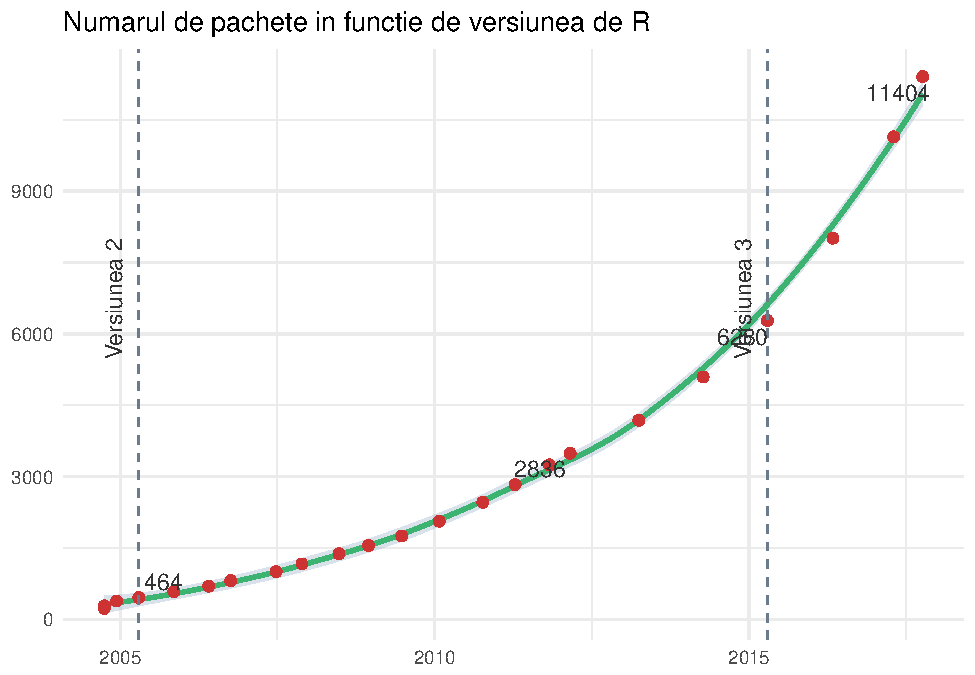
\includegraphics[width=0.8\linewidth]{Lab_1_files/figure-latex/unnamed-chunk-2-1} 

}

\caption{Numarul de pachete din R}\label{fig:unnamed-chunk-2}
\end{figure}

\subsection{\texorpdfstring{Interfața
\texttt{RStudio}}{Interfața RStudio}}\label{interfata-rstudio}

Interfața RStudio (vezi Figura 1) este compusă din patru ferestre:

\begin{itemize}
\tightlist
\item
  \emph{Fereastra de editare} (stânga sus): în această fereastră apar
  fișierele, de tip \texttt{script}, în care utilizatorul dezvoltă
  propriile funcții ori script-uri.\\
\item
  \emph{Fereastra de comandă} sau \emph{consola} (stânga jos): în
  această fereastră sunt executate comenzile R
\item
  \emph{Fereastra cu spațiul de lucru/istoricul} (dreapta sus): conține
  obiectele definite în memorie și istoricul comenzilor folosite
\item
  \emph{Fereastra de explorare} (dreapta jos): în această fereastră ne
  putem deplasa în interiorul repertoriului (tab-ul \emph{Files}), putem
  vedea graficele trasate (tab-ul \emph{Plots}) dar și pachetele
  instalate (tab-ul \emph{Packages}). De asemenea, tot în această
  fereastră putem să și căutăm documentația despre diferite funcții,
  folosind fereastra de ajutor (tab-ul \emph{Help}).
\end{itemize}

\begin{figure}

{\centering 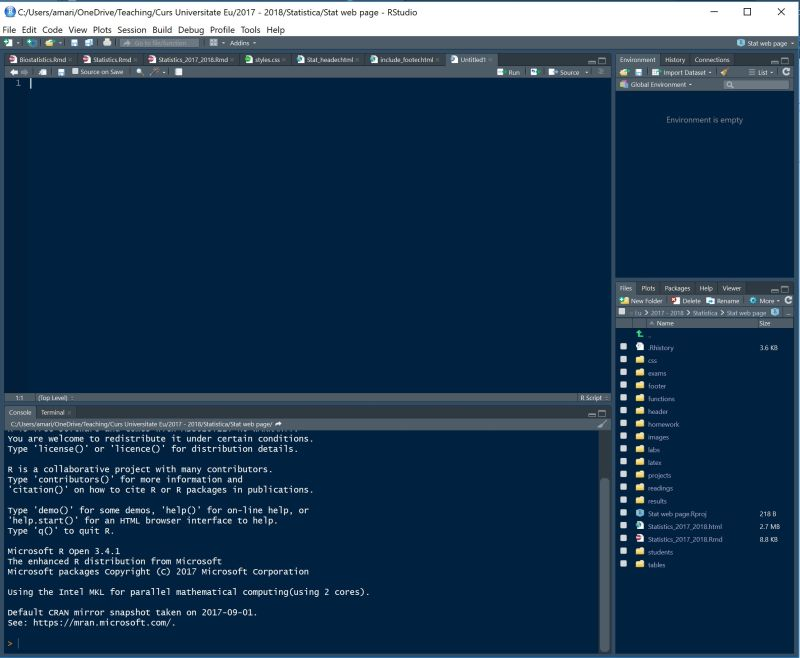
\includegraphics[width=0.8\linewidth]{images/lab1/RStudio2} 

}

\caption{Interfata RStudio}\label{fig:unnamed-chunk-3}
\end{figure}

\subsection{Pachetele ajutătoare}\label{pachetele-ajutatoare}

Pe lângă diferitele pachete conținute în versiunea de bază a programului
\texttt{R} se mai pot instala și pachete suplimentare. Pentru a instala
un pachet suplimentar se apelează comanda:

\begin{Shaded}
\begin{Highlighting}[]
\KeywordTok{install.packages}\NormalTok{(}\StringTok{"nume pachet"}\NormalTok{)}
\end{Highlighting}
\end{Shaded}

Odată ce pachetul este instalat, pentru a încărca pachetul, și prin
urmare funcțiile disponibile în acesta, se apelează comanda:

\begin{Shaded}
\begin{Highlighting}[]
\KeywordTok{library}\NormalTok{(}\StringTok{"nume pachet"}\NormalTok{)}
\end{Highlighting}
\end{Shaded}

Instalarea unui pachet se face o singură dată dar încărcarea acestuia
trebuie făcută de fiecare dată când lansăm o sesiune nouă.

\section{\texorpdfstring{Primele comenzi în
\texttt{R}}{Primele comenzi în R}}\label{primele-comenzi-in-r}

\subsection{Calcul elementar}\label{calcul-elementar}

Programul \texttt{R} poate fi folosit și pe post de calculator (mai
avansat). De exemplu putem face calcule elementare

\begin{Shaded}
\begin{Highlighting}[]
\DecValTok{5} \OperatorTok{-}\StringTok{ }\DecValTok{1} \OperatorTok{+}\StringTok{ }\DecValTok{10}
\NormalTok{[}\DecValTok{1}\NormalTok{] }\DecValTok{14}
\DecValTok{7} \OperatorTok{*}\StringTok{ }\DecValTok{10} \OperatorTok{/}\StringTok{ }\DecValTok{2}
\NormalTok{[}\DecValTok{1}\NormalTok{] }\DecValTok{35}
\KeywordTok{exp}\NormalTok{(}\OperatorTok{-}\FloatTok{2.19}\NormalTok{)}
\NormalTok{[}\DecValTok{1}\NormalTok{] }\FloatTok{0.1119167}
\NormalTok{pi}
\NormalTok{[}\DecValTok{1}\NormalTok{] }\FloatTok{3.141593}
\KeywordTok{sin}\NormalTok{(}\DecValTok{2} \OperatorTok{*}\StringTok{ }\NormalTok{pi}\OperatorTok{/}\DecValTok{3}\NormalTok{)}
\NormalTok{[}\DecValTok{1}\NormalTok{] }\FloatTok{0.8660254}
\end{Highlighting}
\end{Shaded}

De asemenea, rezultatele pot fi stocate într-o variabilă

\begin{Shaded}
\begin{Highlighting}[]
\NormalTok{a =}\StringTok{ }\NormalTok{(}\DecValTok{1}\OperatorTok{+}\KeywordTok{sqrt}\NormalTok{(}\DecValTok{5}\NormalTok{)}\OperatorTok{/}\DecValTok{2}\NormalTok{)}\OperatorTok{/}\DecValTok{2}
\end{Highlighting}
\end{Shaded}

păstrată în memorie (\texttt{a} apare în fereastra de lucru -
\texttt{Environment}) și care poate fi reutilizată ulterior

\begin{Shaded}
\begin{Highlighting}[]
\NormalTok{asq =}\StringTok{ }\KeywordTok{sqrt}\NormalTok{(a)}
\NormalTok{asq}
\NormalTok{[}\DecValTok{1}\NormalTok{] }\FloatTok{1.029086}
\end{Highlighting}
\end{Shaded}

Pentru a șterge toate variabilele din memorie trebuie să folosim comanda
următoare (funcția \texttt{ls()} listează numele obiectelor din memorie
iar comanda \texttt{rm()} șterge obiectele; de asemenea se poate folosi
și comanda \texttt{ls.str()} pentru a lista obiectele împreună cu o
scurtă descriere a lor)

\begin{Shaded}
\begin{Highlighting}[]
\KeywordTok{ls.str}\NormalTok{()}
\KeywordTok{rm}\NormalTok{(}\DataTypeTok{list =} \KeywordTok{ls}\NormalTok{())}
\end{Highlighting}
\end{Shaded}

\subsection{Folosirea documentației}\label{folosirea-documentatiei}

Funcția \texttt{help()} și operatorul de ajutor \texttt{?} ne permite
accesul la paginile de documentația pentru funcțiile, seturile de date
și alte obiecte din R. Pentru a accesa documentația pentru funcția
standard \texttt{mean()} putem să folosim comanda \texttt{help(mean)}
sau \texttt{?mean} în consolă. Pentru a accesa documentația unei funcții
dintr-un pachet care nu este în prezent încărcat (dar este instalat)
trebuie să adăugăm în plus numele pachetului, de exemplu
\texttt{help(rlm,\ package\ =\ "MASS")} iar pentru a accesa documentația
întregului pachet putem folosi comanda
\texttt{help(package\ =\ "MASS")}.

O altă funcție de căutare des utilizată, în special în situația în care
nu știm cu exactitate numele obiectului pe care îl căutăm, este funcția
\texttt{apropos()}. Aceasta permite căutarea obiectelor (inclusiv
funcții), disponibile în pachetele încărcate în sesiunea curentă, după
un șir de caractere specificat (se pot folosi și expresii regulate). De
exemplu dacă apelăm \texttt{apropos("mean")} vom obține toate funcțiile
care conțin șirul de caractere \emph{mean}.

\begin{Shaded}
\begin{Highlighting}[]
\KeywordTok{apropos}\NormalTok{(}\StringTok{"mean"}\NormalTok{) }\CommentTok{# functii care contin mean}
\NormalTok{ [}\DecValTok{1}\NormalTok{] }\StringTok{".colMeans"}      \StringTok{".rowMeans"}      \StringTok{"colMeans"}       \StringTok{"kmeans"}        
\NormalTok{ [}\DecValTok{5}\NormalTok{] }\StringTok{"mean"}           \StringTok{"mean.Date"}      \StringTok{"mean.default"}   \StringTok{"mean.difftime"} 
\NormalTok{ [}\DecValTok{9}\NormalTok{] }\StringTok{"mean.POSIXct"}   \StringTok{"mean.POSIXlt"}   \StringTok{"mean_cl_boot"}   \StringTok{"mean_cl_normal"}
\NormalTok{[}\DecValTok{13}\NormalTok{] }\StringTok{"mean_sdl"}       \StringTok{"mean_se"}        \StringTok{"rowMeans"}       \StringTok{"weighted.mean"} 

\KeywordTok{apropos}\NormalTok{(}\StringTok{"^mean"}\NormalTok{) }\CommentTok{# functii care incep cu mean}
\NormalTok{ [}\DecValTok{1}\NormalTok{] }\StringTok{"mean"}           \StringTok{"mean.Date"}      \StringTok{"mean.default"}   \StringTok{"mean.difftime"} 
\NormalTok{ [}\DecValTok{5}\NormalTok{] }\StringTok{"mean.POSIXct"}   \StringTok{"mean.POSIXlt"}   \StringTok{"mean_cl_boot"}   \StringTok{"mean_cl_normal"}
\NormalTok{ [}\DecValTok{9}\NormalTok{] }\StringTok{"mean_sdl"}       \StringTok{"mean_se"}       
\end{Highlighting}
\end{Shaded}

Următorul tabel prezintă funcțiile de ajutor, cel mai des utilizate:

\begin{longtable}[]{@{}ll@{}}
\caption{Functii folosite pentru ajutor}\tabularnewline
\toprule
\begin{minipage}[b]{0.27\columnwidth}\raggedright\strut
Funcție\strut
\end{minipage} & \begin{minipage}[b]{0.34\columnwidth}\raggedright\strut
Acțiune\strut
\end{minipage}\tabularnewline
\midrule
\endfirsthead
\toprule
\begin{minipage}[b]{0.27\columnwidth}\raggedright\strut
Funcție\strut
\end{minipage} & \begin{minipage}[b]{0.34\columnwidth}\raggedright\strut
Acțiune\strut
\end{minipage}\tabularnewline
\midrule
\endhead
\begin{minipage}[t]{0.27\columnwidth}\raggedright\strut
\texttt{help.start()}\strut
\end{minipage} & \begin{minipage}[t]{0.34\columnwidth}\raggedright\strut
Modul de ajutor general\strut
\end{minipage}\tabularnewline
\begin{minipage}[t]{0.27\columnwidth}\raggedright\strut
\texttt{help("nume")} sau \texttt{?nume}\strut
\end{minipage} & \begin{minipage}[t]{0.34\columnwidth}\raggedright\strut
Documentație privind funcția \emph{nume} (ghilimelele sunt
opționale)\strut
\end{minipage}\tabularnewline
\begin{minipage}[t]{0.27\columnwidth}\raggedright\strut
\texttt{help.search(nume)} sau \texttt{??nume}\strut
\end{minipage} & \begin{minipage}[t]{0.34\columnwidth}\raggedright\strut
Caută sistemul de documentație pentru instanțe în care apare șirul de
caractere \emph{nume}\strut
\end{minipage}\tabularnewline
\begin{minipage}[t]{0.27\columnwidth}\raggedright\strut
\texttt{example("nume")}\strut
\end{minipage} & \begin{minipage}[t]{0.34\columnwidth}\raggedright\strut
Exemple de utilizare ale funcției \emph{nume}\strut
\end{minipage}\tabularnewline
\begin{minipage}[t]{0.27\columnwidth}\raggedright\strut
\texttt{RSiteSearch("nume")}\strut
\end{minipage} & \begin{minipage}[t]{0.34\columnwidth}\raggedright\strut
Caută șirul de caractere \emph{nume} în manualele online și în
arhivă\strut
\end{minipage}\tabularnewline
\begin{minipage}[t]{0.27\columnwidth}\raggedright\strut
\texttt{apropos("nume",\ mode\ =\ "functions")}\strut
\end{minipage} & \begin{minipage}[t]{0.34\columnwidth}\raggedright\strut
Listează toate funcțiile care conțin șirul \emph{nume} în numele
lor\strut
\end{minipage}\tabularnewline
\begin{minipage}[t]{0.27\columnwidth}\raggedright\strut
\texttt{data()}\strut
\end{minipage} & \begin{minipage}[t]{0.34\columnwidth}\raggedright\strut
Listează toate seturile de date disponibile în pachetele încărcate\strut
\end{minipage}\tabularnewline
\begin{minipage}[t]{0.27\columnwidth}\raggedright\strut
\texttt{vignette()}\strut
\end{minipage} & \begin{minipage}[t]{0.34\columnwidth}\raggedright\strut
Listează toate vinietele disponibile\strut
\end{minipage}\tabularnewline
\begin{minipage}[t]{0.27\columnwidth}\raggedright\strut
\texttt{vignette("nume")}\strut
\end{minipage} & \begin{minipage}[t]{0.34\columnwidth}\raggedright\strut
Afișează vinietele corespunzătoare topicului \emph{nume}\strut
\end{minipage}\tabularnewline
\bottomrule
\end{longtable}

\section{Tipuri și structuri de date}\label{tipuri-si-structuri-de-date}

\texttt{R} are cinci tipuri de date principale (atomi), după cum
urmează:

\begin{itemize}
\tightlist
\item
  \textbf{character}: \texttt{"a"}, \texttt{"swc"}
\item
  \textbf{numeric}: \texttt{2}, \texttt{15.5}
\item
  \textbf{integer}: \texttt{2L} (sufix-ul \texttt{L} îi spune R-ului să
  stocheze numărul ca pe un întreg)
\item
  \textbf{logical}: \texttt{TRUE}, \texttt{FALSE}
\item
  \textbf{complex}: \texttt{1+4i} (numere complexe)
\end{itemize}

R pune la dispoziție mai multe funcții cu ajutorul cărora se pot examina
trăsăturile vectorilor sau a altor obiecte, cum ar fi de exemplu

\begin{itemize}
\tightlist
\item
  \texttt{class()} - ce tip de obiect este
\item
  \texttt{typeof()} - care este tipul de date al obiectului
\item
  \texttt{length()} - care este lungimea obiectului
\item
  \texttt{attributes()} - care sunt atributele obiectului (metadata)
\end{itemize}

\begin{Shaded}
\begin{Highlighting}[]
\CommentTok{# Exemplu}
\NormalTok{x <-}\StringTok{ "curs probabilitati si statistica"}
\KeywordTok{typeof}\NormalTok{(x)}
\NormalTok{[}\DecValTok{1}\NormalTok{] }\StringTok{"character"}
\KeywordTok{attributes}\NormalTok{(x)}
\OtherTok{NULL}

\NormalTok{y <-}\StringTok{ }\DecValTok{1}\OperatorTok{:}\DecValTok{10}
\NormalTok{y}
\NormalTok{ [}\DecValTok{1}\NormalTok{]  }\DecValTok{1}  \DecValTok{2}  \DecValTok{3}  \DecValTok{4}  \DecValTok{5}  \DecValTok{6}  \DecValTok{7}  \DecValTok{8}  \DecValTok{9} \DecValTok{10}
\KeywordTok{typeof}\NormalTok{(y)}
\NormalTok{[}\DecValTok{1}\NormalTok{] }\StringTok{"integer"}
\KeywordTok{length}\NormalTok{(y)}
\NormalTok{[}\DecValTok{1}\NormalTok{] }\DecValTok{10}

\NormalTok{z <-}\StringTok{ }\KeywordTok{as.numeric}\NormalTok{(y)}
\NormalTok{z}
\NormalTok{ [}\DecValTok{1}\NormalTok{]  }\DecValTok{1}  \DecValTok{2}  \DecValTok{3}  \DecValTok{4}  \DecValTok{5}  \DecValTok{6}  \DecValTok{7}  \DecValTok{8}  \DecValTok{9} \DecValTok{10}
\KeywordTok{typeof}\NormalTok{(z)}
\NormalTok{[}\DecValTok{1}\NormalTok{] }\StringTok{"double"}
\end{Highlighting}
\end{Shaded}

În limbajul \texttt{R} regăsim mai multe \textbf{structuri de date}.
Printre acestea enumerăm

\begin{itemize}
\tightlist
\item
  vectorii (structuri atomice)
\item
  listele
\item
  matricele
\item
  data frame
\item
  factori
\end{itemize}

\subsection{Scalari și vectori}\label{scalari-si-vectori}

Cel mai de bază tip de obiect în R este vectorul. Una dintre regulile
principale ale vectorilor este că aceștia pot conține numai obiecte de
același tip, cu alte cuvinte putem avea doar vectori de tip caracter,
numeric, logic, etc.. În cazul în care încercăm să combinăm diferite
tipuri de date, acestea vor fi forțate la tipul cel mai flexibil.
Tipurile de la cel mai puțin la cele mai flexibile sunt: logice,
întregi, numerice și caractere.

\subsubsection{Metode de construcție a
vectorilor}\label{metode-de-constructie-a-vectorilor}

Putem crea vectori fără elemente (empty) cu ajutorul funcției
\texttt{vector()}, modul default este \emph{logical} dar acesta se poate
schimba în funcție de necesitate.

\begin{Shaded}
\begin{Highlighting}[]
\KeywordTok{vector}\NormalTok{() }\CommentTok{# vector logic gol}
\KeywordTok{logical}\NormalTok{(}\DecValTok{0}\NormalTok{)}
\KeywordTok{vector}\NormalTok{(}\StringTok{"character"}\NormalTok{, }\DataTypeTok{length =} \DecValTok{5}\NormalTok{) }\CommentTok{# vector de caractere cu 5 elemente}
\NormalTok{[}\DecValTok{1}\NormalTok{] }\StringTok{""} \StringTok{""} \StringTok{""} \StringTok{""} \StringTok{""}
\KeywordTok{character}\NormalTok{(}\DecValTok{5}\NormalTok{) }\CommentTok{# acelasi lucru dar in mod direct}
\NormalTok{[}\DecValTok{1}\NormalTok{] }\StringTok{""} \StringTok{""} \StringTok{""} \StringTok{""} \StringTok{""}
\KeywordTok{numeric}\NormalTok{(}\DecValTok{5}\NormalTok{)   }\CommentTok{# vector numeric cu 5 elemente}
\NormalTok{[}\DecValTok{1}\NormalTok{] }\DecValTok{0} \DecValTok{0} \DecValTok{0} \DecValTok{0} \DecValTok{0}
\KeywordTok{logical}\NormalTok{(}\DecValTok{5}\NormalTok{)   }\CommentTok{# vector logic cu 5 elemente}
\NormalTok{[}\DecValTok{1}\NormalTok{] }\OtherTok{FALSE} \OtherTok{FALSE} \OtherTok{FALSE} \OtherTok{FALSE} \OtherTok{FALSE}
\end{Highlighting}
\end{Shaded}

Putem crea vectori specificând în mod direct conținutul acestora. Pentru
aceasta folosim funcția \texttt{c()} de concatenare:

\begin{Shaded}
\begin{Highlighting}[]
\NormalTok{x <-}\StringTok{ }\KeywordTok{c}\NormalTok{(}\FloatTok{0.5}\NormalTok{, }\FloatTok{0.6}\NormalTok{)       ## numeric}
\NormalTok{x <-}\StringTok{ }\KeywordTok{c}\NormalTok{(}\OtherTok{TRUE}\NormalTok{, }\OtherTok{FALSE}\NormalTok{)    ## logical}
\NormalTok{x <-}\StringTok{ }\KeywordTok{c}\NormalTok{(T, F)           ## logical}
\NormalTok{x <-}\StringTok{ }\KeywordTok{c}\NormalTok{(}\StringTok{"a"}\NormalTok{, }\StringTok{"b"}\NormalTok{, }\StringTok{"c"}\NormalTok{)  ## character}
\NormalTok{x <-}\StringTok{ }\DecValTok{9}\OperatorTok{:}\DecValTok{29}\NormalTok{              ## integer}
\NormalTok{x <-}\StringTok{ }\KeywordTok{c}\NormalTok{(}\DecValTok{1}\OperatorTok{+}\NormalTok{0i, }\DecValTok{2}\OperatorTok{+}\NormalTok{4i)     ## complex}
\end{Highlighting}
\end{Shaded}

Funcția poate fi folosită de asemenea și pentru (combinarea) adăugarea
de elemente la un vector

\begin{Shaded}
\begin{Highlighting}[]
\NormalTok{z <-}\StringTok{ }\KeywordTok{c}\NormalTok{(}\StringTok{"Sandra"}\NormalTok{, }\StringTok{"Traian"}\NormalTok{, }\StringTok{"Ionel"}\NormalTok{)}
\NormalTok{z <-}\StringTok{ }\KeywordTok{c}\NormalTok{(z, }\StringTok{"Ana"}\NormalTok{)}
\NormalTok{z}
\NormalTok{[}\DecValTok{1}\NormalTok{] }\StringTok{"Sandra"} \StringTok{"Traian"} \StringTok{"Ionel"}  \StringTok{"Ana"}   
\NormalTok{z <-}\StringTok{ }\KeywordTok{c}\NormalTok{(}\StringTok{"George"}\NormalTok{, z)}
\NormalTok{z}
\NormalTok{[}\DecValTok{1}\NormalTok{] }\StringTok{"George"} \StringTok{"Sandra"} \StringTok{"Traian"} \StringTok{"Ionel"}  \StringTok{"Ana"}   
\end{Highlighting}
\end{Shaded}

O altă funcție des folosită în crearea vectorilor, în special a celor
care au repetiții, este funcția \texttt{rep()}. Pentru a vedea
documentația acestei funcții apelați \texttt{help(rep)}. De exemplu,
pentru a crea un vector de lungime \texttt{5} cu elemente de \texttt{0}
este suficient să scriem

\begin{Shaded}
\begin{Highlighting}[]
\KeywordTok{rep}\NormalTok{(}\DecValTok{0}\NormalTok{, }\DecValTok{5}\NormalTok{)}
\NormalTok{[}\DecValTok{1}\NormalTok{] }\DecValTok{0} \DecValTok{0} \DecValTok{0} \DecValTok{0} \DecValTok{0}
\end{Highlighting}
\end{Shaded}

Dacă în plus vrem să creăm vectorul 1, 2, 3, 1, 2, 3, 1, 2, 3, 1, 2, 3,
1, 2, 3 sau 1, 1, 1, 1, 1, 2, 2, 2, 2, 2, 3, 3, 3, 3, 3 atunci

\begin{Shaded}
\begin{Highlighting}[]
\KeywordTok{rep}\NormalTok{(}\KeywordTok{c}\NormalTok{(}\DecValTok{1}\NormalTok{,}\DecValTok{2}\NormalTok{,}\DecValTok{3}\NormalTok{), }\DecValTok{5}\NormalTok{)}
\NormalTok{ [}\DecValTok{1}\NormalTok{] }\DecValTok{1} \DecValTok{2} \DecValTok{3} \DecValTok{1} \DecValTok{2} \DecValTok{3} \DecValTok{1} \DecValTok{2} \DecValTok{3} \DecValTok{1} \DecValTok{2} \DecValTok{3} \DecValTok{1} \DecValTok{2} \DecValTok{3}

\KeywordTok{rep}\NormalTok{(}\KeywordTok{c}\NormalTok{(}\DecValTok{1}\NormalTok{,}\DecValTok{2}\NormalTok{,}\DecValTok{3}\NormalTok{), }\DataTypeTok{each =} \DecValTok{5}\NormalTok{)}
\NormalTok{ [}\DecValTok{1}\NormalTok{] }\DecValTok{1} \DecValTok{1} \DecValTok{1} \DecValTok{1} \DecValTok{1} \DecValTok{2} \DecValTok{2} \DecValTok{2} \DecValTok{2} \DecValTok{2} \DecValTok{3} \DecValTok{3} \DecValTok{3} \DecValTok{3} \DecValTok{3}
\end{Highlighting}
\end{Shaded}

Ce se întâmplă dacă apelăm \texttt{rep(c(1,2,3),\ 1:3)} ?

În cazul în care vrem să creăm un vector care are elementele egal
depărtate între ele, de exemplu 1.3, 2.3, 3.3, 4.3, 5.3, atunci putem
folosi funcția \texttt{seq()}:

\begin{Shaded}
\begin{Highlighting}[]
\KeywordTok{seq}\NormalTok{(}\DecValTok{1}\NormalTok{, }\DecValTok{10}\NormalTok{, }\DecValTok{1}\NormalTok{)}
\NormalTok{ [}\DecValTok{1}\NormalTok{]  }\DecValTok{1}  \DecValTok{2}  \DecValTok{3}  \DecValTok{4}  \DecValTok{5}  \DecValTok{6}  \DecValTok{7}  \DecValTok{8}  \DecValTok{9} \DecValTok{10}
\DecValTok{1}\OperatorTok{:}\DecValTok{10} \CommentTok{# acelasi rezultat}
\NormalTok{ [}\DecValTok{1}\NormalTok{]  }\DecValTok{1}  \DecValTok{2}  \DecValTok{3}  \DecValTok{4}  \DecValTok{5}  \DecValTok{6}  \DecValTok{7}  \DecValTok{8}  \DecValTok{9} \DecValTok{10}

\KeywordTok{seq}\NormalTok{(}\DecValTok{1}\NormalTok{, }\DecValTok{10}\NormalTok{, }\DataTypeTok{length.out =} \DecValTok{15}\NormalTok{)}
\NormalTok{ [}\DecValTok{1}\NormalTok{]  }\FloatTok{1.000000}  \FloatTok{1.642857}  \FloatTok{2.285714}  \FloatTok{2.928571}  \FloatTok{3.571429}  \FloatTok{4.214286}  \FloatTok{4.857143}
\NormalTok{ [}\DecValTok{8}\NormalTok{]  }\FloatTok{5.500000}  \FloatTok{6.142857}  \FloatTok{6.785714}  \FloatTok{7.428571}  \FloatTok{8.071429}  \FloatTok{8.714286}  \FloatTok{9.357143}
\NormalTok{[}\DecValTok{15}\NormalTok{] }\FloatTok{10.000000}
\end{Highlighting}
\end{Shaded}

\subsubsection{Operații cu vectori}\label{operatii-cu-vectori}

Operațiile elementare pe care le puteam face cu scalari (adunarea
\texttt{+}, scăderea \texttt{-}, înmulțirea \texttt{*}, împărțirea
\texttt{/} și ridicarea la putere \texttt{\^{}}) putem să le facem și cu
vectori (între vectori sau între vectori și scalari).

\begin{Shaded}
\begin{Highlighting}[]
\NormalTok{a =}\StringTok{ }\DecValTok{1}\OperatorTok{:}\DecValTok{4}
\NormalTok{b =}\StringTok{ }\KeywordTok{c}\NormalTok{(}\DecValTok{5}\NormalTok{,}\DecValTok{5}\NormalTok{,}\DecValTok{6}\NormalTok{,}\DecValTok{7}\NormalTok{)}

\NormalTok{a}\OperatorTok{+}\NormalTok{b  }\CommentTok{# adunarea }
\NormalTok{[}\DecValTok{1}\NormalTok{]  }\DecValTok{6}  \DecValTok{7}  \DecValTok{9} \DecValTok{11}
\NormalTok{a}\OperatorTok{+}\DecValTok{10} \CommentTok{# adunarea cu scalari}
\NormalTok{[}\DecValTok{1}\NormalTok{] }\DecValTok{11} \DecValTok{12} \DecValTok{13} \DecValTok{14}

\NormalTok{a}\OperatorTok{-}\NormalTok{b  }\CommentTok{# scaderea}
\NormalTok{[}\DecValTok{1}\NormalTok{] }\OperatorTok{-}\DecValTok{4} \OperatorTok{-}\DecValTok{3} \OperatorTok{-}\DecValTok{3} \OperatorTok{-}\DecValTok{3}
\NormalTok{a}\OperatorTok{-}\DecValTok{15} \CommentTok{# scaderea cu scalari}
\NormalTok{[}\DecValTok{1}\NormalTok{] }\OperatorTok{-}\DecValTok{14} \OperatorTok{-}\DecValTok{13} \OperatorTok{-}\DecValTok{12} \OperatorTok{-}\DecValTok{11}

\NormalTok{a}\OperatorTok{*}\NormalTok{b }\CommentTok{# inmultirea}
\NormalTok{[}\DecValTok{1}\NormalTok{]  }\DecValTok{5} \DecValTok{10} \DecValTok{18} \DecValTok{28}
\NormalTok{a}\OperatorTok{*}\DecValTok{3} \CommentTok{# inmultirea cu scalari}
\NormalTok{[}\DecValTok{1}\NormalTok{]  }\DecValTok{3}  \DecValTok{6}  \DecValTok{9} \DecValTok{12}

\NormalTok{a}\OperatorTok{/}\NormalTok{b }\CommentTok{# impartirea}
\NormalTok{[}\DecValTok{1}\NormalTok{] }\FloatTok{0.2000000} \FloatTok{0.4000000} \FloatTok{0.5000000} \FloatTok{0.5714286}
\NormalTok{a}\OperatorTok{/}\DecValTok{100} \CommentTok{# impartirea la scalari}
\NormalTok{[}\DecValTok{1}\NormalTok{] }\FloatTok{0.01} \FloatTok{0.02} \FloatTok{0.03} \FloatTok{0.04}

\NormalTok{a}\OperatorTok{^}\NormalTok{b }\CommentTok{# ridicarea la putere}
\NormalTok{[}\DecValTok{1}\NormalTok{]     }\DecValTok{1}    \DecValTok{32}   \DecValTok{729} \DecValTok{16384}
\NormalTok{a}\OperatorTok{^}\DecValTok{7} \CommentTok{# ridicarea la putere cu scalari}
\NormalTok{[}\DecValTok{1}\NormalTok{]     }\DecValTok{1}   \DecValTok{128}  \DecValTok{2187} \DecValTok{16384}
\end{Highlighting}
\end{Shaded}

Observăm că atunci când facem o operație cu scalar, se aplică scalarul
la fiecare element al vectorului.

Funcțiile elementare, \texttt{exp()}, \texttt{log()}, \texttt{sin()},
\texttt{cos()}, \texttt{tan()}, \texttt{asin()}, \texttt{acos()},
\texttt{atan()}, etc. sunt funcții vectoriale în R, prin urmare pot fi
aplicate unor vectori.

\begin{Shaded}
\begin{Highlighting}[]
\NormalTok{x =}\StringTok{ }\KeywordTok{seq}\NormalTok{(}\DecValTok{0}\NormalTok{, }\DecValTok{2}\OperatorTok{*}\NormalTok{pi, }\DataTypeTok{length.out =} \DecValTok{20}\NormalTok{)}

\KeywordTok{exp}\NormalTok{(x)}
\NormalTok{ [}\DecValTok{1}\NormalTok{]   }\FloatTok{1.000000}   \FloatTok{1.391934}   \FloatTok{1.937480}   \FloatTok{2.696843}   \FloatTok{3.753827}   \FloatTok{5.225078}
\NormalTok{ [}\DecValTok{7}\NormalTok{]   }\FloatTok{7.272963}  \FloatTok{10.123483}  \FloatTok{14.091217}  \FloatTok{19.614041}  \FloatTok{27.301445}  \FloatTok{38.001803}
\NormalTok{[}\DecValTok{13}\NormalTok{]  }\FloatTok{52.895992}  \FloatTok{73.627716} \FloatTok{102.484902} \FloatTok{142.652193} \FloatTok{198.562402} \FloatTok{276.385707}
\NormalTok{[}\DecValTok{19}\NormalTok{] }\FloatTok{384.710592} \FloatTok{535.491656}
\KeywordTok{sin}\NormalTok{(x)}
\NormalTok{ [}\DecValTok{1}\NormalTok{]  }\FloatTok{0.000000e+00}  \FloatTok{3.246995e-01}  \FloatTok{6.142127e-01}  \FloatTok{8.371665e-01}  \FloatTok{9.694003e-01}
\NormalTok{ [}\DecValTok{6}\NormalTok{]  }\FloatTok{9.965845e-01}  \FloatTok{9.157733e-01}  \FloatTok{7.357239e-01}  \FloatTok{4.759474e-01}  \FloatTok{1.645946e-01}
\NormalTok{[}\DecValTok{11}\NormalTok{] }\OperatorTok{-}\FloatTok{1.645946e-01} \OperatorTok{-}\FloatTok{4.759474e-01} \OperatorTok{-}\FloatTok{7.357239e-01} \OperatorTok{-}\FloatTok{9.157733e-01} \OperatorTok{-}\FloatTok{9.965845e-01}
\NormalTok{[}\DecValTok{16}\NormalTok{] }\OperatorTok{-}\FloatTok{9.694003e-01} \OperatorTok{-}\FloatTok{8.371665e-01} \OperatorTok{-}\FloatTok{6.142127e-01} \OperatorTok{-}\FloatTok{3.246995e-01} \OperatorTok{-}\FloatTok{2.449213e-16}
\KeywordTok{tan}\NormalTok{(x)}
\NormalTok{ [}\DecValTok{1}\NormalTok{]  }\FloatTok{0.000000e+00}  \FloatTok{3.433004e-01}  \FloatTok{7.783312e-01}  \FloatTok{1.530614e+00}  \FloatTok{3.948911e+00}
\NormalTok{ [}\DecValTok{6}\NormalTok{] }\OperatorTok{-}\FloatTok{1.206821e+01} \OperatorTok{-}\FloatTok{2.279770e+00} \OperatorTok{-}\FloatTok{1.086290e+00} \OperatorTok{-}\FloatTok{5.411729e-01} \OperatorTok{-}\FloatTok{1.668705e-01}
\NormalTok{[}\DecValTok{11}\NormalTok{]  }\FloatTok{1.668705e-01}  \FloatTok{5.411729e-01}  \FloatTok{1.086290e+00}  \FloatTok{2.279770e+00}  \FloatTok{1.206821e+01}
\NormalTok{[}\DecValTok{16}\NormalTok{] }\OperatorTok{-}\FloatTok{3.948911e+00} \OperatorTok{-}\FloatTok{1.530614e+00} \OperatorTok{-}\FloatTok{7.783312e-01} \OperatorTok{-}\FloatTok{3.433004e-01} \OperatorTok{-}\FloatTok{2.449294e-16}
\KeywordTok{atan}\NormalTok{(x)}
\NormalTok{ [}\DecValTok{1}\NormalTok{] }\FloatTok{0.0000000} \FloatTok{0.3193732} \FloatTok{0.5843392} \FloatTok{0.7814234} \FloatTok{0.9234752} \FloatTok{1.0268631} \FloatTok{1.1039613}
\NormalTok{ [}\DecValTok{8}\NormalTok{] }\FloatTok{1.1630183} \FloatTok{1.2094043} \FloatTok{1.2466533} \FloatTok{1.2771443} \FloatTok{1.3025194} \FloatTok{1.3239406} \FloatTok{1.3422495}
\NormalTok{[}\DecValTok{15}\NormalTok{] }\FloatTok{1.3580684} \FloatTok{1.3718664} \FloatTok{1.3840031} \FloatTok{1.3947585} \FloatTok{1.4043537} \FloatTok{1.4129651}
\end{Highlighting}
\end{Shaded}

Alte funcții utile des întâlnite în manipularea vectorilor numerici
sunt: \texttt{min()}, \texttt{max()}, \texttt{sum()}, \texttt{mean()},
\texttt{sd()}, \texttt{length()}, \texttt{round()}, \texttt{ceiling()},
\texttt{floor()}, \texttt{\%\%} (operația modulo), \texttt{\%/\%} (div),
\texttt{table()}, \texttt{unique()}. Pentru mai multe informații privind
modul lor de întrebuințare apelați \texttt{help(nume\_functie)} sau
\texttt{?nume\_functie}.

\begin{Shaded}
\begin{Highlighting}[]
\KeywordTok{length}\NormalTok{(x)}
\NormalTok{[}\DecValTok{1}\NormalTok{] }\DecValTok{20}
\KeywordTok{min}\NormalTok{(x)}
\NormalTok{[}\DecValTok{1}\NormalTok{] }\DecValTok{0}
\KeywordTok{sum}\NormalTok{(x)}
\NormalTok{[}\DecValTok{1}\NormalTok{] }\FloatTok{62.83185}
\KeywordTok{mean}\NormalTok{(x)}
\NormalTok{[}\DecValTok{1}\NormalTok{] }\FloatTok{3.141593}

\KeywordTok{round}\NormalTok{(x, }\DataTypeTok{digits =} \DecValTok{4}\NormalTok{)}
\NormalTok{ [}\DecValTok{1}\NormalTok{] }\FloatTok{0.0000} \FloatTok{0.3307} \FloatTok{0.6614} \FloatTok{0.9921} \FloatTok{1.3228} \FloatTok{1.6535} \FloatTok{1.9842} \FloatTok{2.3149} \FloatTok{2.6456} \FloatTok{2.9762}
\NormalTok{[}\DecValTok{11}\NormalTok{] }\FloatTok{3.3069} \FloatTok{3.6376} \FloatTok{3.9683} \FloatTok{4.2990} \FloatTok{4.6297} \FloatTok{4.9604} \FloatTok{5.2911} \FloatTok{5.6218} \FloatTok{5.9525} \FloatTok{6.2832}

\NormalTok{y =}\StringTok{  }\KeywordTok{c}\NormalTok{(}\StringTok{"M"}\NormalTok{, }\StringTok{"M"}\NormalTok{, }\StringTok{"F"}\NormalTok{, }\StringTok{"F"}\NormalTok{, }\StringTok{"F"}\NormalTok{, }\StringTok{"M"}\NormalTok{, }\StringTok{"F"}\NormalTok{, }\StringTok{"M"}\NormalTok{, }\StringTok{"F"}\NormalTok{)}
\KeywordTok{unique}\NormalTok{(y)}
\NormalTok{[}\DecValTok{1}\NormalTok{] }\StringTok{"M"} \StringTok{"F"}
\KeywordTok{table}\NormalTok{(y)}
\NormalTok{y}
\NormalTok{F M }
\DecValTok{5} \DecValTok{4} 
\end{Highlighting}
\end{Shaded}

\subsubsection{Metode de indexare a
vectorilor}\label{metode-de-indexare-a-vectorilor}

Sunt multe situațiile în care nu vrem să efectuăm operații pe întreg
vectorul ci pe o submulțime de valori ale lui selecționate în funcție de
anumite proprietăți. Putem, de exemplu, să ne dorim să accesăm al 2-lea
element al vectorului sau toate elementele mai mari decât o anumită
valoare. Pentru aceasta vom folosi operația de \emph{indexare} folosind
parantezele pătrate \texttt{{[}{]}}.

În general, sunt două tehnici principale de indexare: indexarea numerică
și indexarea logică.

Atunci când folosim indexarea numerică, inserăm între parantezele
pătrate un vector numeric ce corespunde elementelor pe care vrem să le
accesăm sub forma \texttt{x{[}index{]}} (\texttt{x} este vectorul
inițial iar \texttt{index} este vectorul de indici):

\begin{Shaded}
\begin{Highlighting}[]
\NormalTok{x =}\StringTok{ }\KeywordTok{seq}\NormalTok{(}\DecValTok{1}\NormalTok{, }\DecValTok{10}\NormalTok{, }\DataTypeTok{length.out =} \DecValTok{21}\NormalTok{) }\CommentTok{# vectorul initial }

\NormalTok{x[}\DecValTok{1}\NormalTok{] }\CommentTok{# accesam primul element}
\NormalTok{[}\DecValTok{1}\NormalTok{] }\DecValTok{1}
\NormalTok{x[}\KeywordTok{c}\NormalTok{(}\DecValTok{2}\NormalTok{,}\DecValTok{5}\NormalTok{,}\DecValTok{9}\NormalTok{)] }\CommentTok{# accesam elementul de pe pozitia 2, 5 si 9}
\NormalTok{[}\DecValTok{1}\NormalTok{] }\FloatTok{1.45} \FloatTok{2.80} \FloatTok{4.60}
\NormalTok{x[}\DecValTok{4}\OperatorTok{:}\DecValTok{10}\NormalTok{] }\CommentTok{# accesam toate elementele deintre pozitiile 4 si 9}
\NormalTok{[}\DecValTok{1}\NormalTok{] }\FloatTok{2.35} \FloatTok{2.80} \FloatTok{3.25} \FloatTok{3.70} \FloatTok{4.15} \FloatTok{4.60} \FloatTok{5.05}
\end{Highlighting}
\end{Shaded}

Putem folosi orice vector de indici atât timp cât el conține numere
întregi. Putem să accesăm elementele vectorului \texttt{x} și de mai
multe ori:

\begin{Shaded}
\begin{Highlighting}[]
\NormalTok{x[}\KeywordTok{c}\NormalTok{(}\DecValTok{1}\NormalTok{,}\DecValTok{1}\NormalTok{,}\DecValTok{2}\NormalTok{,}\DecValTok{2}\NormalTok{)]}
\NormalTok{[}\DecValTok{1}\NormalTok{] }\FloatTok{1.00} \FloatTok{1.00} \FloatTok{1.45} \FloatTok{1.45}
\end{Highlighting}
\end{Shaded}

De asemenea dacă vrem să afișăm toate elementele mai puțin elementul de
pe poziția \texttt{i} atunci putem folosi indexare cu numere negative
(această metodă este folositoare și în cazul în care vrem să ștergem un
element al vectorului):

\begin{Shaded}
\begin{Highlighting}[]
\NormalTok{x[}\OperatorTok{-}\DecValTok{5}\NormalTok{] }\CommentTok{# toate elementele mai putin cel de pe pozitia 5 }
\NormalTok{ [}\DecValTok{1}\NormalTok{]  }\FloatTok{1.00}  \FloatTok{1.45}  \FloatTok{1.90}  \FloatTok{2.35}  \FloatTok{3.25}  \FloatTok{3.70}  \FloatTok{4.15}  \FloatTok{4.60}  \FloatTok{5.05}  \FloatTok{5.50}  \FloatTok{5.95}
\NormalTok{[}\DecValTok{12}\NormalTok{]  }\FloatTok{6.40}  \FloatTok{6.85}  \FloatTok{7.30}  \FloatTok{7.75}  \FloatTok{8.20}  \FloatTok{8.65}  \FloatTok{9.10}  \FloatTok{9.55} \FloatTok{10.00}
\NormalTok{x[}\OperatorTok{-}\NormalTok{(}\DecValTok{1}\OperatorTok{:}\DecValTok{3}\NormalTok{)] }\CommentTok{# toate elementele mai putin primele 3}
\NormalTok{ [}\DecValTok{1}\NormalTok{]  }\FloatTok{2.35}  \FloatTok{2.80}  \FloatTok{3.25}  \FloatTok{3.70}  \FloatTok{4.15}  \FloatTok{4.60}  \FloatTok{5.05}  \FloatTok{5.50}  \FloatTok{5.95}  \FloatTok{6.40}  \FloatTok{6.85}
\NormalTok{[}\DecValTok{12}\NormalTok{]  }\FloatTok{7.30}  \FloatTok{7.75}  \FloatTok{8.20}  \FloatTok{8.65}  \FloatTok{9.10}  \FloatTok{9.55} \FloatTok{10.00}
\NormalTok{x =}\StringTok{ }\NormalTok{x[}\OperatorTok{-}\DecValTok{10}\NormalTok{] }\CommentTok{# vectorul x fara elementul de pe pozitia a 10-a}
\end{Highlighting}
\end{Shaded}

A doua modilitate de indexare este cu ajutorul vectorilor logici. Atunci
când indexăm cu un vector logic acesta trebuie să aibă aceeași lungime
ca și vectorul pe care vrem să îl indexăm.

Să presupunem că vrem să extragem din vectorul \texttt{x} doar
elementele care verifică o anumită proprietate, spre exemplu sunt mai
mari decât 3, atunci:

\begin{Shaded}
\begin{Highlighting}[]
\NormalTok{x}\OperatorTok{>}\DecValTok{3} \CommentTok{# un vector logic care ne arata care elemente sunt mai mari decat 3}
\NormalTok{ [}\DecValTok{1}\NormalTok{] }\OtherTok{FALSE} \OtherTok{FALSE} \OtherTok{FALSE} \OtherTok{FALSE} \OtherTok{FALSE}  \OtherTok{TRUE}  \OtherTok{TRUE}  \OtherTok{TRUE}  \OtherTok{TRUE}  \OtherTok{TRUE}  \OtherTok{TRUE}
\NormalTok{[}\DecValTok{12}\NormalTok{]  }\OtherTok{TRUE}  \OtherTok{TRUE}  \OtherTok{TRUE}  \OtherTok{TRUE}  \OtherTok{TRUE}  \OtherTok{TRUE}  \OtherTok{TRUE}  \OtherTok{TRUE}  \OtherTok{TRUE}
\NormalTok{x[x}\OperatorTok{>}\DecValTok{3}\NormalTok{] }\CommentTok{# elementele din x care sunt mai mari decat 3}
\NormalTok{ [}\DecValTok{1}\NormalTok{]  }\FloatTok{3.25}  \FloatTok{3.70}  \FloatTok{4.15}  \FloatTok{4.60}  \FloatTok{5.50}  \FloatTok{5.95}  \FloatTok{6.40}  \FloatTok{6.85}  \FloatTok{7.30}  \FloatTok{7.75}  \FloatTok{8.20}
\NormalTok{[}\DecValTok{12}\NormalTok{]  }\FloatTok{8.65}  \FloatTok{9.10}  \FloatTok{9.55} \FloatTok{10.00}
\end{Highlighting}
\end{Shaded}

Pentru a determina care sunt toate elementele din \texttt{x} cuprinse
între 5 și 19 putem să folosim operații cu operatori logici:

\begin{Shaded}
\begin{Highlighting}[]
\NormalTok{x[(x}\OperatorTok{>}\DecValTok{5}\NormalTok{)}\OperatorTok{&}\NormalTok{(x}\OperatorTok{<}\DecValTok{19}\NormalTok{)]}
\NormalTok{ [}\DecValTok{1}\NormalTok{]  }\FloatTok{5.50}  \FloatTok{5.95}  \FloatTok{6.40}  \FloatTok{6.85}  \FloatTok{7.30}  \FloatTok{7.75}  \FloatTok{8.20}  \FloatTok{8.65}  \FloatTok{9.10}  \FloatTok{9.55} \FloatTok{10.00}
\end{Highlighting}
\end{Shaded}

O listă a operatorilor logici din R se găsește în tabelul următor:

\begin{longtable}[]{@{}ll@{}}
\caption{Operatori logici}\tabularnewline
\toprule
Operator & Descriere\tabularnewline
\midrule
\endfirsthead
\toprule
Operator & Descriere\tabularnewline
\midrule
\endhead
\texttt{==} & Egal\tabularnewline
\texttt{!=} & Diferit\tabularnewline
\texttt{\textless{}} & Mai mic\tabularnewline
\texttt{\textless{}=} & Mai mic sau egal\tabularnewline
\texttt{\textgreater{}} & Mai mare\tabularnewline
\texttt{\textgreater{}=} & Mai mare sau egal\tabularnewline
\texttt{\textbar{}} sau \texttt{\textbar{}\textbar{}} & Sau (primul are
valori vectoriale al doilea scalare)\tabularnewline
\texttt{\&} sau \texttt{\&\&} & Și (primul are valori vectoriale al
doilea scalare)\tabularnewline
\texttt{!} & Negație\tabularnewline
\texttt{\%in\%} & În mulțimea\tabularnewline
\bottomrule
\end{longtable}

\begin{Shaded}
\begin{Highlighting}[]
\NormalTok{x =}\StringTok{ }\KeywordTok{seq}\NormalTok{(}\DecValTok{1}\NormalTok{,}\DecValTok{10}\NormalTok{,}\DataTypeTok{length.out =} \DecValTok{8}\NormalTok{)}
\NormalTok{x }\OperatorTok{==}\StringTok{ }\DecValTok{3}
\NormalTok{[}\DecValTok{1}\NormalTok{] }\OtherTok{FALSE} \OtherTok{FALSE} \OtherTok{FALSE} \OtherTok{FALSE} \OtherTok{FALSE} \OtherTok{FALSE} \OtherTok{FALSE} \OtherTok{FALSE}
\NormalTok{x }\OperatorTok{!=}\StringTok{ }\DecValTok{3}
\NormalTok{[}\DecValTok{1}\NormalTok{] }\OtherTok{TRUE} \OtherTok{TRUE} \OtherTok{TRUE} \OtherTok{TRUE} \OtherTok{TRUE} \OtherTok{TRUE} \OtherTok{TRUE} \OtherTok{TRUE}
\NormalTok{x }\OperatorTok{<=}\StringTok{ }\FloatTok{8.6}
\NormalTok{[}\DecValTok{1}\NormalTok{]  }\OtherTok{TRUE}  \OtherTok{TRUE}  \OtherTok{TRUE}  \OtherTok{TRUE}  \OtherTok{TRUE}  \OtherTok{TRUE} \OtherTok{FALSE} \OtherTok{FALSE}
\NormalTok{(x}\OperatorTok{<}\DecValTok{8}\NormalTok{) }\OperatorTok{&}\StringTok{ }\NormalTok{(x}\OperatorTok{>}\DecValTok{2}\NormalTok{)}
\NormalTok{[}\DecValTok{1}\NormalTok{] }\OtherTok{FALSE}  \OtherTok{TRUE}  \OtherTok{TRUE}  \OtherTok{TRUE}  \OtherTok{TRUE}  \OtherTok{TRUE} \OtherTok{FALSE} \OtherTok{FALSE}
\NormalTok{(x}\OperatorTok{<}\DecValTok{8}\NormalTok{) }\OperatorTok{&&}\StringTok{ }\NormalTok{(x}\OperatorTok{>}\DecValTok{2}\NormalTok{)}
\NormalTok{[}\DecValTok{1}\NormalTok{] }\OtherTok{FALSE}
\NormalTok{(x}\OperatorTok{<}\DecValTok{7}\NormalTok{) }\OperatorTok{|}\StringTok{ }\NormalTok{(x}\OperatorTok{>}\DecValTok{3}\NormalTok{)}
\NormalTok{[}\DecValTok{1}\NormalTok{] }\OtherTok{TRUE} \OtherTok{TRUE} \OtherTok{TRUE} \OtherTok{TRUE} \OtherTok{TRUE} \OtherTok{TRUE} \OtherTok{TRUE} \OtherTok{TRUE}
\NormalTok{(x}\OperatorTok{<}\DecValTok{7}\NormalTok{) }\OperatorTok{||}\StringTok{ }\NormalTok{(x}\OperatorTok{>}\DecValTok{3}\NormalTok{)}
\NormalTok{[}\DecValTok{1}\NormalTok{] }\OtherTok{TRUE}
\NormalTok{x }\OperatorTok\StringTok{ }\KeywordTok{c}\NormalTok{(}\DecValTok{1}\NormalTok{,}\DecValTok{9}\NormalTok{)}
\NormalTok{[}\DecValTok{1}\NormalTok{]  }\OtherTok{TRUE} \OtherTok{FALSE} \OtherTok{FALSE} \OtherTok{FALSE} \OtherTok{FALSE} \OtherTok{FALSE} \OtherTok{FALSE} \OtherTok{FALSE}
\end{Highlighting}
\end{Shaded}

\begin{rmdexercise}
Să presupunem că am înregistrat în fiecare zi, pe parcursul a 4
săptămâni (de Luni până Duminică), numărul de minute petrecute la
telefonul mobil (convorbiri + utilizare) și am obținut următoarele
valori: 106, 123, 123, 111, 125, 113, 130, 113, 114, 100, 120, 130, 118,
114, 127, 112, 121, 114, 120, 119, 127, 114, 108, 127, 131, 157, 102,
133. Ne întrebăm: care sunt zilele din săptămână în care am vorbit cel
mai mult? dar cel mai puțin? dar zilele în care am vorbit mai mult de
120 de minute?
\end{rmdexercise}

\subsection{Matrice}\label{matrice}

Matricele sunt structuri de date care extind vectorii și sunt folosite
la representarea datelor de același tip în două dimensiuni. Matricele
sunt similare tablourilor din Excel și pot fi văzute ca vectori cu două
atribute suplimentare: numărul de linii (\emph{rows}) și numărul de
coloane (\emph{columns}).

\begin{figure}

{\centering 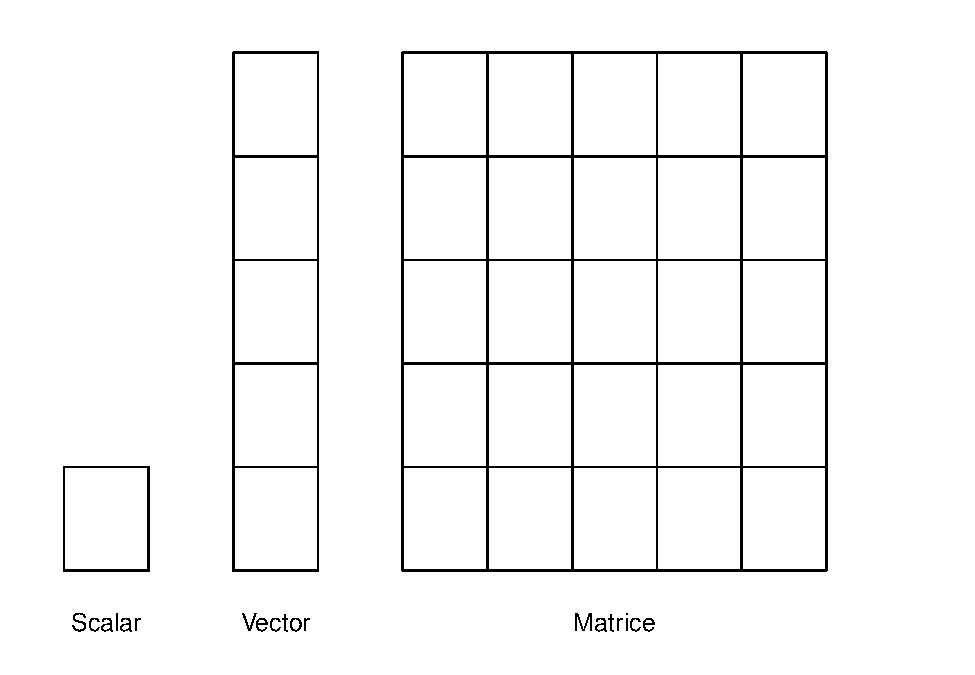
\includegraphics[width=0.8\linewidth]{Lab_1_files/figure-latex/unnamed-chunk-28-1} 

}

\caption{Scalari, Vectori, Matrice}\label{fig:unnamed-chunk-28}
\end{figure}

Indexarea liniilor și a coloanelor pentru o matrice începe cu 1. De
exemplu, elementul din colțul din stânga sus al unei matrice este notat
cu \texttt{x{[}1,1{]}}. De asemenea este important de menționat că
stocarea (internă) a metricelor se face pe coloane în sensul că prima
oară este stocată coloana 1, apoi coloana 2, etc..

Există mai multe moduri de creare a unei matrici în R. Funcțiile cele
mai uzuale sunt prezentate în tabelul de mai jos. Cum matricele sunt
combinații de vectori, fiecare funcție primește ca argument unul sau mai
mulți vectori (toți de același tip) și ne întoarce o matrice.

\begin{longtable}[]{@{}lll@{}}
\caption{Functii care permit crearea matricelor}\tabularnewline
\toprule
\begin{minipage}[b]{0.19\columnwidth}\raggedright\strut
Funcție\strut
\end{minipage} & \begin{minipage}[b]{0.27\columnwidth}\raggedright\strut
Descriere\strut
\end{minipage} & \begin{minipage}[b]{0.41\columnwidth}\raggedright\strut
Exemple\strut
\end{minipage}\tabularnewline
\midrule
\endfirsthead
\toprule
\begin{minipage}[b]{0.19\columnwidth}\raggedright\strut
Funcție\strut
\end{minipage} & \begin{minipage}[b]{0.27\columnwidth}\raggedright\strut
Descriere\strut
\end{minipage} & \begin{minipage}[b]{0.41\columnwidth}\raggedright\strut
Exemple\strut
\end{minipage}\tabularnewline
\midrule
\endhead
\begin{minipage}[t]{0.19\columnwidth}\raggedright\strut
\texttt{cbind(a,\ b,\ c)}\strut
\end{minipage} & \begin{minipage}[t]{0.27\columnwidth}\raggedright\strut
Combină vectorii ca și coloane într-o matrice\strut
\end{minipage} & \begin{minipage}[t]{0.41\columnwidth}\raggedright\strut
\texttt{cbind(1:5,\ 6:10,\ 11:15)}\strut
\end{minipage}\tabularnewline
\begin{minipage}[t]{0.19\columnwidth}\raggedright\strut
\texttt{rbind(a,\ b,\ c)}\strut
\end{minipage} & \begin{minipage}[t]{0.27\columnwidth}\raggedright\strut
Combină vectorii ca și linii într-o matrice\strut
\end{minipage} & \begin{minipage}[t]{0.41\columnwidth}\raggedright\strut
\texttt{rbind(1:5,\ 6:10,\ 11:15)}\strut
\end{minipage}\tabularnewline
\begin{minipage}[t]{0.19\columnwidth}\raggedright\strut
\texttt{matrix(x,\ nrow,\ ncol,\ byrow)}\strut
\end{minipage} & \begin{minipage}[t]{0.27\columnwidth}\raggedright\strut
Crează o matrice dintr-un vector \texttt{x}\strut
\end{minipage} & \begin{minipage}[t]{0.41\columnwidth}\raggedright\strut
\texttt{matrix(x\ =\ 1:12,\ nrow\ =\ 3,\ ncol\ =\ 4)}\strut
\end{minipage}\tabularnewline
\bottomrule
\end{longtable}

Pentru a vedea ce obținem atunci când folosim funcțiile \texttt{cbind()}
și \texttt{rbind()} să considerăm exemplele următoare:

\newpage

\begin{Shaded}
\begin{Highlighting}[]
\NormalTok{x <-}\StringTok{ }\DecValTok{1}\OperatorTok{:}\DecValTok{5}
\NormalTok{y <-}\StringTok{ }\DecValTok{6}\OperatorTok{:}\DecValTok{10}
\NormalTok{z <-}\StringTok{ }\DecValTok{11}\OperatorTok{:}\DecValTok{15}

\CommentTok{# Cream o matrice cu x, y si z ca si coloane}
\KeywordTok{cbind}\NormalTok{(x, y, z)}
\NormalTok{     x  y  z}
\NormalTok{[}\DecValTok{1}\NormalTok{,] }\DecValTok{1}  \DecValTok{6} \DecValTok{11}
\NormalTok{[}\DecValTok{2}\NormalTok{,] }\DecValTok{2}  \DecValTok{7} \DecValTok{12}
\NormalTok{[}\DecValTok{3}\NormalTok{,] }\DecValTok{3}  \DecValTok{8} \DecValTok{13}
\NormalTok{[}\DecValTok{4}\NormalTok{,] }\DecValTok{4}  \DecValTok{9} \DecValTok{14}
\NormalTok{[}\DecValTok{5}\NormalTok{,] }\DecValTok{5} \DecValTok{10} \DecValTok{15}

\CommentTok{# Cream o matrice in care x, y si z sunt linii}
\KeywordTok{rbind}\NormalTok{(x, y, z)}
\NormalTok{  [,}\DecValTok{1}\NormalTok{] [,}\DecValTok{2}\NormalTok{] [,}\DecValTok{3}\NormalTok{] [,}\DecValTok{4}\NormalTok{] [,}\DecValTok{5}\NormalTok{]}
\NormalTok{x    }\DecValTok{1}    \DecValTok{2}    \DecValTok{3}    \DecValTok{4}    \DecValTok{5}
\NormalTok{y    }\DecValTok{6}    \DecValTok{7}    \DecValTok{8}    \DecValTok{9}   \DecValTok{10}
\NormalTok{z   }\DecValTok{11}   \DecValTok{12}   \DecValTok{13}   \DecValTok{14}   \DecValTok{15}
\end{Highlighting}
\end{Shaded}

Funcția \texttt{matrix()} crează o matrice plecând de la un singur
vector. Funcția are patru valori de intrare: \texttt{data} -- un vector
cu date, \texttt{nrow} -- numărul de linii pe care le vrem în matrice,
\texttt{ncol} -- numărul de coloane pe care să le aibe matricea și
\texttt{byrow} -- o valoare logică care permite crearea matricei pe
linii (nu pe coloane cum este default-ul).

\begin{Shaded}
\begin{Highlighting}[]
\CommentTok{# matrice cu 5 linii si 2 coloane}
\KeywordTok{matrix}\NormalTok{(}\DataTypeTok{data =} \DecValTok{1}\OperatorTok{:}\DecValTok{10}\NormalTok{,}
       \DataTypeTok{nrow =} \DecValTok{5}\NormalTok{,}
       \DataTypeTok{ncol =} \DecValTok{2}\NormalTok{)}
\NormalTok{     [,}\DecValTok{1}\NormalTok{] [,}\DecValTok{2}\NormalTok{]}
\NormalTok{[}\DecValTok{1}\NormalTok{,]    }\DecValTok{1}    \DecValTok{6}
\NormalTok{[}\DecValTok{2}\NormalTok{,]    }\DecValTok{2}    \DecValTok{7}
\NormalTok{[}\DecValTok{3}\NormalTok{,]    }\DecValTok{3}    \DecValTok{8}
\NormalTok{[}\DecValTok{4}\NormalTok{,]    }\DecValTok{4}    \DecValTok{9}
\NormalTok{[}\DecValTok{5}\NormalTok{,]    }\DecValTok{5}   \DecValTok{10}

\CommentTok{# matrice cu 2 linii si 5 coloane}
\KeywordTok{matrix}\NormalTok{(}\DataTypeTok{data =} \DecValTok{1}\OperatorTok{:}\DecValTok{10}\NormalTok{,}
       \DataTypeTok{nrow =} \DecValTok{2}\NormalTok{,}
       \DataTypeTok{ncol =} \DecValTok{5}\NormalTok{)}
\NormalTok{     [,}\DecValTok{1}\NormalTok{] [,}\DecValTok{2}\NormalTok{] [,}\DecValTok{3}\NormalTok{] [,}\DecValTok{4}\NormalTok{] [,}\DecValTok{5}\NormalTok{]}
\NormalTok{[}\DecValTok{1}\NormalTok{,]    }\DecValTok{1}    \DecValTok{3}    \DecValTok{5}    \DecValTok{7}    \DecValTok{9}
\NormalTok{[}\DecValTok{2}\NormalTok{,]    }\DecValTok{2}    \DecValTok{4}    \DecValTok{6}    \DecValTok{8}   \DecValTok{10}

\CommentTok{# aceeasi matrice cu 2 linii si 5 coloane, umpluta pe linii }
\KeywordTok{matrix}\NormalTok{(}\DataTypeTok{data =} \DecValTok{1}\OperatorTok{:}\DecValTok{10}\NormalTok{,}
       \DataTypeTok{nrow =} \DecValTok{2}\NormalTok{,}
       \DataTypeTok{ncol =} \DecValTok{5}\NormalTok{,}
       \DataTypeTok{byrow =} \OtherTok{TRUE}\NormalTok{)}
\NormalTok{     [,}\DecValTok{1}\NormalTok{] [,}\DecValTok{2}\NormalTok{] [,}\DecValTok{3}\NormalTok{] [,}\DecValTok{4}\NormalTok{] [,}\DecValTok{5}\NormalTok{]}
\NormalTok{[}\DecValTok{1}\NormalTok{,]    }\DecValTok{1}    \DecValTok{2}    \DecValTok{3}    \DecValTok{4}    \DecValTok{5}
\NormalTok{[}\DecValTok{2}\NormalTok{,]    }\DecValTok{6}    \DecValTok{7}    \DecValTok{8}    \DecValTok{9}   \DecValTok{10}
\end{Highlighting}
\end{Shaded}

Operațiile uzuale cu vectori se aplică și matricelor. Pe lângă acestea
avem la dispoziție și operații de algebră liniară clasice, cum ar fi
determinarea dimensiunii acestora, transpunerea matricelor sau
înmulțirea lor:

\begin{Shaded}
\begin{Highlighting}[]
\NormalTok{m =}\StringTok{ }\KeywordTok{matrix}\NormalTok{(}\DataTypeTok{data =} \DecValTok{1}\OperatorTok{:}\DecValTok{10}\NormalTok{,}
       \DataTypeTok{nrow =} \DecValTok{2}\NormalTok{,}
       \DataTypeTok{ncol =} \DecValTok{5}\NormalTok{)}
\NormalTok{m}
\NormalTok{     [,}\DecValTok{1}\NormalTok{] [,}\DecValTok{2}\NormalTok{] [,}\DecValTok{3}\NormalTok{] [,}\DecValTok{4}\NormalTok{] [,}\DecValTok{5}\NormalTok{]}
\NormalTok{[}\DecValTok{1}\NormalTok{,]    }\DecValTok{1}    \DecValTok{3}    \DecValTok{5}    \DecValTok{7}    \DecValTok{9}
\NormalTok{[}\DecValTok{2}\NormalTok{,]    }\DecValTok{2}    \DecValTok{4}    \DecValTok{6}    \DecValTok{8}   \DecValTok{10}

\KeywordTok{dim}\NormalTok{(m) }\CommentTok{# dimensiunea matricei}
\NormalTok{[}\DecValTok{1}\NormalTok{] }\DecValTok{2} \DecValTok{5}
\KeywordTok{nrow}\NormalTok{(m) }\CommentTok{# numarul de linii}
\NormalTok{[}\DecValTok{1}\NormalTok{] }\DecValTok{2}
\KeywordTok{ncol}\NormalTok{(m) }\CommentTok{# numarul de coloane}
\NormalTok{[}\DecValTok{1}\NormalTok{] }\DecValTok{5}

\NormalTok{tpm =}\StringTok{ }\KeywordTok{t}\NormalTok{(m) }\CommentTok{# transpusa}
\NormalTok{tpm}
\NormalTok{     [,}\DecValTok{1}\NormalTok{] [,}\DecValTok{2}\NormalTok{]}
\NormalTok{[}\DecValTok{1}\NormalTok{,]    }\DecValTok{1}    \DecValTok{2}
\NormalTok{[}\DecValTok{2}\NormalTok{,]    }\DecValTok{3}    \DecValTok{4}
\NormalTok{[}\DecValTok{3}\NormalTok{,]    }\DecValTok{5}    \DecValTok{6}
\NormalTok{[}\DecValTok{4}\NormalTok{,]    }\DecValTok{7}    \DecValTok{8}
\NormalTok{[}\DecValTok{5}\NormalTok{,]    }\DecValTok{9}   \DecValTok{10}

\NormalTok{m }\OperatorTok\StringTok{ }\NormalTok{tpm }\CommentTok{# inmultirea matricelor}
\NormalTok{     [,}\DecValTok{1}\NormalTok{] [,}\DecValTok{2}\NormalTok{]}
\NormalTok{[}\DecValTok{1}\NormalTok{,]  }\DecValTok{165}  \DecValTok{190}
\NormalTok{[}\DecValTok{2}\NormalTok{,]  }\DecValTok{190}  \DecValTok{220}
\end{Highlighting}
\end{Shaded}

Metodele de indexare discutate pentru vectori se aplică și în cazul
matricelor (\texttt{{[},{]}}) numai că acum în loc să folosim un vector
să indexăm putem să folosim doi vectori. Sintaxa are structura generală
\texttt{m{[}linii,\ coloane{]}} unde \texttt{linii} și \texttt{coloane}
sunt vectori cu valori întregi.

\begin{Shaded}
\begin{Highlighting}[]
\NormalTok{m =}\StringTok{ }\KeywordTok{matrix}\NormalTok{(}\DecValTok{1}\OperatorTok{:}\DecValTok{20}\NormalTok{, }\DataTypeTok{nrow =} \DecValTok{4}\NormalTok{, }\DataTypeTok{byrow =} \OtherTok{TRUE}\NormalTok{)}

\CommentTok{# Linia 1}
\NormalTok{m[}\DecValTok{1}\NormalTok{, ]}
\NormalTok{[}\DecValTok{1}\NormalTok{] }\DecValTok{1} \DecValTok{2} \DecValTok{3} \DecValTok{4} \DecValTok{5}

\CommentTok{# Coloana 5}
\NormalTok{m[, }\DecValTok{5}\NormalTok{]}
\NormalTok{[}\DecValTok{1}\NormalTok{]  }\DecValTok{5} \DecValTok{10} \DecValTok{15} \DecValTok{20}

\CommentTok{# Liniile 2, 3 si coloanele 3, 4}
\NormalTok{m[}\DecValTok{2}\OperatorTok{:}\DecValTok{3}\NormalTok{, }\DecValTok{3}\OperatorTok{:}\DecValTok{4}\NormalTok{]}
\NormalTok{     [,}\DecValTok{1}\NormalTok{] [,}\DecValTok{2}\NormalTok{]}
\NormalTok{[}\DecValTok{1}\NormalTok{,]    }\DecValTok{8}    \DecValTok{9}
\NormalTok{[}\DecValTok{2}\NormalTok{,]   }\DecValTok{13}   \DecValTok{14}

\CommentTok{# Elementele din coloana 3 care corespund liniilor pentru care elementele }
\CommentTok{# de pe prima coloana sunt > 3}
\NormalTok{m[m[,}\DecValTok{1}\NormalTok{]}\OperatorTok{>}\DecValTok{3}\NormalTok{, }\DecValTok{3}\NormalTok{]}
\NormalTok{[}\DecValTok{1}\NormalTok{]  }\DecValTok{8} \DecValTok{13} \DecValTok{18}
\end{Highlighting}
\end{Shaded}

\subsection{Liste}\label{liste}

Spre deosebire de vectori în care toate elementele trebuie să aibă
același tip de dată, structura de dată din R de tip listă (\emph{list})
permite combinarea obiectelor de mai multe tipuri. Cu alte cuvinte, o
listă poate avea primul element un scalar, al doilea un vector, al
treilea o matrice iar cel de-al patrulea element poate fi o altă listă.
Tehnic listele sunt tot vectori, vectorii pe care i-am văzut anterior se
numesc \emph{vectori atomici}, deoarece elementele lor nu se pot diviza,
pe când listele se numesc \emph{vectori recursivi}.

Ca un prim exemplu să considerăm cazul unei baze de date de angajați.
Pentru fiecare angajat, ne dorim să stocăm numele angajatului (șir de
caractere), salariul (valoare numerică) și o valoare de tip logic care
poate reprezenta apartenența într-o asociație. Pentru crearea listei
folosim funcția \texttt{list()}:

\begin{Shaded}
\begin{Highlighting}[]
\NormalTok{a =}\StringTok{ }\KeywordTok{list}\NormalTok{(}\DataTypeTok{nume =} \StringTok{"Ionel"}\NormalTok{, }\DataTypeTok{salariu =} \DecValTok{1500}\NormalTok{, }\DataTypeTok{apartenenta =}\NormalTok{ T)}
\NormalTok{a}
\OperatorTok{$}\NormalTok{nume}
\NormalTok{[}\DecValTok{1}\NormalTok{] }\StringTok{"Ionel"}

\OperatorTok{$}\NormalTok{salariu}
\NormalTok{[}\DecValTok{1}\NormalTok{] }\DecValTok{1500}

\OperatorTok{$}\NormalTok{apartenenta}
\NormalTok{[}\DecValTok{1}\NormalTok{] }\OtherTok{TRUE}
\KeywordTok{str}\NormalTok{(a) }\CommentTok{# structura listei}
\NormalTok{List of }\DecValTok{3}
 \OperatorTok{$}\StringTok{ }\NormalTok{nume       }\OperatorTok{:}\StringTok{ }\NormalTok{chr }\StringTok{"Ionel"}
 \OperatorTok{$}\StringTok{ }\NormalTok{salariu    }\OperatorTok{:}\StringTok{ }\NormalTok{num }\DecValTok{1500}
 \OperatorTok{$}\StringTok{ }\NormalTok{apartenenta}\OperatorTok{:}\StringTok{ }\NormalTok{logi }\OtherTok{TRUE}
\KeywordTok{names}\NormalTok{(a) }\CommentTok{# numele listei}
\NormalTok{[}\DecValTok{1}\NormalTok{] }\StringTok{"nume"}        \StringTok{"salariu"}     \StringTok{"apartenenta"}
\end{Highlighting}
\end{Shaded}

Numele componentelor listei \texttt{a} (nume, salariu, apartenenta) nu
sunt obligatorii dar cu toate acestea pentru claritate sunt indicate:

\begin{Shaded}
\begin{Highlighting}[]
\NormalTok{a2 =}\StringTok{ }\KeywordTok{list}\NormalTok{(}\StringTok{"Ionel"}\NormalTok{, }\DecValTok{1500}\NormalTok{, T)}
\NormalTok{a2}
\NormalTok{[[}\DecValTok{1}\NormalTok{]]}
\NormalTok{[}\DecValTok{1}\NormalTok{] }\StringTok{"Ionel"}

\NormalTok{[[}\DecValTok{2}\NormalTok{]]}
\NormalTok{[}\DecValTok{1}\NormalTok{] }\DecValTok{1500}

\NormalTok{[[}\DecValTok{3}\NormalTok{]]}
\NormalTok{[}\DecValTok{1}\NormalTok{] }\OtherTok{TRUE}
\end{Highlighting}
\end{Shaded}

Deoarece listele sunt vectori ele pot fi create și prin intermediul
funcției \texttt{vector()}:

\begin{Shaded}
\begin{Highlighting}[]
\NormalTok{z <-}\StringTok{ }\KeywordTok{vector}\NormalTok{(}\DataTypeTok{mode=}\StringTok{"list"}\NormalTok{)}
\NormalTok{z}
\KeywordTok{list}\NormalTok{()}
\NormalTok{z[[}\StringTok{"a"}\NormalTok{]] =}\StringTok{ }\DecValTok{3}
\NormalTok{z}
\OperatorTok{$}\NormalTok{a}
\NormalTok{[}\DecValTok{1}\NormalTok{] }\DecValTok{3}
\end{Highlighting}
\end{Shaded}

\subsubsection{Indexarea listelor}\label{indexarea-listelor}

Elementele unei liste pot fi accesate în diferite moduri. Dacă dorim să
extragem primul element al listei atunci vom folosi indexarea care
folosește o singură pereche de paranteze pătrate \texttt{{[}{]}}

\begin{Shaded}
\begin{Highlighting}[]
\NormalTok{a[}\DecValTok{1}\NormalTok{]}
\OperatorTok{$}\NormalTok{nume}
\NormalTok{[}\DecValTok{1}\NormalTok{] }\StringTok{"Ionel"}
\NormalTok{a[}\DecValTok{2}\NormalTok{]}
\OperatorTok{$}\NormalTok{salariu}
\NormalTok{[}\DecValTok{1}\NormalTok{] }\DecValTok{1500}

\CommentTok{# ce obtinem cand extragem un element al listei a ?}
\KeywordTok{str}\NormalTok{(a[}\DecValTok{1}\NormalTok{]) }
\NormalTok{List of }\DecValTok{1}
 \OperatorTok{$}\StringTok{ }\NormalTok{nume}\OperatorTok{:}\StringTok{ }\NormalTok{chr }\StringTok{"Ionel"}
\end{Highlighting}
\end{Shaded}

În cazul în care vrem să accesăm structura de date corespunzătoare
elementului i al listei vom folosi două perechi de paranteze pătrate
\texttt{{[}{[}{]}{]}} sau în cazul în care lista are nume operatorul
\texttt{\$} urmat de numele elementului i.

\begin{Shaded}
\begin{Highlighting}[]
\NormalTok{a[[}\DecValTok{1}\NormalTok{]]}
\NormalTok{[}\DecValTok{1}\NormalTok{] }\StringTok{"Ionel"}
\NormalTok{a[[}\DecValTok{2}\NormalTok{]]}
\NormalTok{[}\DecValTok{1}\NormalTok{] }\DecValTok{1500}

\NormalTok{a}\OperatorTok{$}\NormalTok{nume}
\NormalTok{[}\DecValTok{1}\NormalTok{] }\StringTok{"Ionel"}
\NormalTok{a[[}\StringTok{"nume"}\NormalTok{]]}
\NormalTok{[}\DecValTok{1}\NormalTok{] }\StringTok{"Ionel"}
\end{Highlighting}
\end{Shaded}

Operațiile de adăugare, respectiv ștergere, a elementelor unei liste
sunt des întâlnite.

Putem adăuga elemente după ce o listă a fost creată folosind numele
componentei

\begin{Shaded}
\begin{Highlighting}[]
\NormalTok{z =}\StringTok{ }\KeywordTok{list}\NormalTok{(}\DataTypeTok{a =} \StringTok{"abc"}\NormalTok{, }\DataTypeTok{b =} \DecValTok{111}\NormalTok{, }\DataTypeTok{c =} \KeywordTok{c}\NormalTok{(}\OtherTok{TRUE}\NormalTok{, }\OtherTok{FALSE}\NormalTok{))}
\NormalTok{z}
\OperatorTok{$}\NormalTok{a}
\NormalTok{[}\DecValTok{1}\NormalTok{] }\StringTok{"abc"}

\OperatorTok{$}\NormalTok{b}
\NormalTok{[}\DecValTok{1}\NormalTok{] }\DecValTok{111}

\OperatorTok{$}\NormalTok{c}
\NormalTok{[}\DecValTok{1}\NormalTok{]  }\OtherTok{TRUE} \OtherTok{FALSE}
\NormalTok{z}\OperatorTok{$}\NormalTok{d =}\StringTok{ "un nou element"}
\NormalTok{z}
\OperatorTok{$}\NormalTok{a}
\NormalTok{[}\DecValTok{1}\NormalTok{] }\StringTok{"abc"}

\OperatorTok{$}\NormalTok{b}
\NormalTok{[}\DecValTok{1}\NormalTok{] }\DecValTok{111}

\OperatorTok{$}\NormalTok{c}
\NormalTok{[}\DecValTok{1}\NormalTok{]  }\OtherTok{TRUE} \OtherTok{FALSE}

\OperatorTok{$}\NormalTok{d}
\NormalTok{[}\DecValTok{1}\NormalTok{] }\StringTok{"un nou element"}
\end{Highlighting}
\end{Shaded}

sau indexare vectorială

\begin{Shaded}
\begin{Highlighting}[]
\NormalTok{z[[}\DecValTok{5}\NormalTok{]] =}\StringTok{ }\DecValTok{200}
\NormalTok{z[}\DecValTok{6}\OperatorTok{:}\DecValTok{7}\NormalTok{] =}\StringTok{ }\KeywordTok{c}\NormalTok{(}\StringTok{"unu"}\NormalTok{, }\StringTok{"doi"}\NormalTok{)}
\NormalTok{z}
\OperatorTok{$}\NormalTok{a}
\NormalTok{[}\DecValTok{1}\NormalTok{] }\StringTok{"abc"}

\OperatorTok{$}\NormalTok{b}
\NormalTok{[}\DecValTok{1}\NormalTok{] }\DecValTok{111}

\OperatorTok{$}\NormalTok{c}
\NormalTok{[}\DecValTok{1}\NormalTok{]  }\OtherTok{TRUE} \OtherTok{FALSE}

\OperatorTok{$}\NormalTok{d}
\NormalTok{[}\DecValTok{1}\NormalTok{] }\StringTok{"un nou element"}

\NormalTok{[[}\DecValTok{5}\NormalTok{]]}
\NormalTok{[}\DecValTok{1}\NormalTok{] }\DecValTok{200}

\NormalTok{[[}\DecValTok{6}\NormalTok{]]}
\NormalTok{[}\DecValTok{1}\NormalTok{] }\StringTok{"unu"}

\NormalTok{[[}\DecValTok{7}\NormalTok{]]}
\NormalTok{[}\DecValTok{1}\NormalTok{] }\StringTok{"doi"}
\end{Highlighting}
\end{Shaded}

Putem șterge o componentă a listei atribuindu-i valoarea \texttt{NULL}:

\begin{Shaded}
\begin{Highlighting}[]
\NormalTok{z[}\DecValTok{4}\NormalTok{] =}\StringTok{ }\OtherTok{NULL}
\NormalTok{z}
\OperatorTok{$}\NormalTok{a}
\NormalTok{[}\DecValTok{1}\NormalTok{] }\StringTok{"abc"}

\OperatorTok{$}\NormalTok{b}
\NormalTok{[}\DecValTok{1}\NormalTok{] }\DecValTok{111}

\OperatorTok{$}\NormalTok{c}
\NormalTok{[}\DecValTok{1}\NormalTok{]  }\OtherTok{TRUE} \OtherTok{FALSE}

\NormalTok{[[}\DecValTok{4}\NormalTok{]]}
\NormalTok{[}\DecValTok{1}\NormalTok{] }\DecValTok{200}

\NormalTok{[[}\DecValTok{5}\NormalTok{]]}
\NormalTok{[}\DecValTok{1}\NormalTok{] }\StringTok{"unu"}

\NormalTok{[[}\DecValTok{6}\NormalTok{]]}
\NormalTok{[}\DecValTok{1}\NormalTok{] }\StringTok{"doi"}
\end{Highlighting}
\end{Shaded}

Putem de asemenea să concatenăm două liste folosind funcția \texttt{c()}
și să determinăm lungimea noii liste cu funcția \texttt{length()}.

\begin{Shaded}
\begin{Highlighting}[]
\NormalTok{l1 =}\StringTok{ }\KeywordTok{list}\NormalTok{(}\DecValTok{1}\OperatorTok{:}\DecValTok{10}\NormalTok{, }\KeywordTok{matrix}\NormalTok{(}\DecValTok{1}\OperatorTok{:}\DecValTok{6}\NormalTok{, }\DataTypeTok{ncol =} \DecValTok{3}\NormalTok{), }\KeywordTok{c}\NormalTok{(T, F))}
\NormalTok{l2 =}\StringTok{ }\KeywordTok{list}\NormalTok{(}\KeywordTok{c}\NormalTok{(}\StringTok{"Ionel"}\NormalTok{, }\StringTok{"Maria"}\NormalTok{), }\KeywordTok{seq}\NormalTok{(}\DecValTok{1}\NormalTok{,}\DecValTok{10}\NormalTok{,}\DecValTok{2}\NormalTok{))}

\NormalTok{l3 =}\StringTok{ }\KeywordTok{c}\NormalTok{(l1, l2)}
\KeywordTok{length}\NormalTok{(l3)}
\NormalTok{[}\DecValTok{1}\NormalTok{] }\DecValTok{5}
\KeywordTok{str}\NormalTok{(l3)}
\NormalTok{List of }\DecValTok{5}
 \OperatorTok{$}\StringTok{ }\ErrorTok{:}\StringTok{ }\NormalTok{int [}\DecValTok{1}\OperatorTok{:}\DecValTok{10}\NormalTok{] }\DecValTok{1} \DecValTok{2} \DecValTok{3} \DecValTok{4} \DecValTok{5} \DecValTok{6} \DecValTok{7} \DecValTok{8} \DecValTok{9} \DecValTok{10}
 \OperatorTok{$}\StringTok{ }\ErrorTok{:}\StringTok{ }\NormalTok{int [}\DecValTok{1}\OperatorTok{:}\DecValTok{2}\NormalTok{, }\DecValTok{1}\OperatorTok{:}\DecValTok{3}\NormalTok{] }\DecValTok{1} \DecValTok{2} \DecValTok{3} \DecValTok{4} \DecValTok{5} \DecValTok{6}
 \OperatorTok{$}\StringTok{ }\ErrorTok{:}\StringTok{ }\NormalTok{logi [}\DecValTok{1}\OperatorTok{:}\DecValTok{2}\NormalTok{] }\OtherTok{TRUE} \OtherTok{FALSE}
 \OperatorTok{$}\StringTok{ }\ErrorTok{:}\StringTok{ }\NormalTok{chr [}\DecValTok{1}\OperatorTok{:}\DecValTok{2}\NormalTok{] }\StringTok{"Ionel"} \StringTok{"Maria"}
 \OperatorTok{$}\StringTok{ }\ErrorTok{:}\StringTok{ }\NormalTok{num [}\DecValTok{1}\OperatorTok{:}\DecValTok{5}\NormalTok{] }\DecValTok{1} \DecValTok{3} \DecValTok{5} \DecValTok{7} \DecValTok{9}
\end{Highlighting}
\end{Shaded}

\subsection{Data frame-uri}\label{data-frame-uri}

La nivel intuitiv, o structură de date de tip \emph{data frame} este ca
o matrice, având o structură bidimensională cu linii și coloane. Cu
toate acestea ea diferă de structura de date de tip matrice prin faptul
că fiecare coloană poate avea tipuri de date diferite. Spre exemplu, o
coloană poate să conțină valori numerice pe când o alta, valori de tip
caracter sau logic. Din punct de vedere tehnic, o structură de tip data
frame este o listă a cărei componente sunt vectori (atomici) de lungimi
egale.

Pentru a crea un dataframe din vectori putem folosi funcția
\texttt{data.frame()}. Această funcție funcționează similar cu funcția
\texttt{list()} sau \texttt{cbind()}, diferența față de \texttt{cbind()}
este că avem posibilitatea să dăm nume coloanelor atunci când le unim.
Dată fiind flexibilitatea acestei structuri de date, majoritatea
seturilor de date din R sunt stocate sub formă de dataframe (această
structură de date este și cea mai des întâlnită în analiza statistică).

Să creăm un dataframe simplu numit \texttt{survey} folosind funcția
\texttt{data.frame()}:

\begin{Shaded}
\begin{Highlighting}[]
\NormalTok{survey <-}\StringTok{ }\KeywordTok{data.frame}\NormalTok{(}\StringTok{"index"}\NormalTok{ =}\StringTok{ }\KeywordTok{c}\NormalTok{(}\DecValTok{1}\NormalTok{, }\DecValTok{2}\NormalTok{, }\DecValTok{3}\NormalTok{, }\DecValTok{4}\NormalTok{, }\DecValTok{5}\NormalTok{),}
                     \StringTok{"sex"}\NormalTok{ =}\StringTok{ }\KeywordTok{c}\NormalTok{(}\StringTok{"m"}\NormalTok{, }\StringTok{"m"}\NormalTok{, }\StringTok{"m"}\NormalTok{, }\StringTok{"f"}\NormalTok{, }\StringTok{"f"}\NormalTok{),}
                     \StringTok{"age"}\NormalTok{ =}\StringTok{ }\KeywordTok{c}\NormalTok{(}\DecValTok{99}\NormalTok{, }\DecValTok{46}\NormalTok{, }\DecValTok{23}\NormalTok{, }\DecValTok{54}\NormalTok{, }\DecValTok{23}\NormalTok{))}
\NormalTok{survey}
\NormalTok{  index sex age}
\DecValTok{1}     \DecValTok{1}\NormalTok{   m  }\DecValTok{99}
\DecValTok{2}     \DecValTok{2}\NormalTok{   m  }\DecValTok{46}
\DecValTok{3}     \DecValTok{3}\NormalTok{   m  }\DecValTok{23}
\DecValTok{4}     \DecValTok{4}\NormalTok{   f  }\DecValTok{54}
\DecValTok{5}     \DecValTok{5}\NormalTok{   f  }\DecValTok{23}
\end{Highlighting}
\end{Shaded}

Funcția \texttt{data.frame()} prezintă un argument specific numit
\texttt{stringsAsFactors} care permite convertirea coloanelor ce conțin
elemente de tip caracter într-un tip de obiect numit \textbf{factor}. Un
factor este o variabilă nominală care poate lua un număr bine definit de
valori. De exemplu, putem crea o variabilă de tip factor \emph{sex} care
poate lua doar două valori: \emph{masculin} și \emph{feminin}.
Comportamentul implicit al funcției \texttt{data.frame()}
(\texttt{stringAsFactors\ =\ TRUE}) transformă automat coloanele de tip
caracter în factor, motiv pentru care trebuie să includem argumentul
\texttt{stringsAsFactors\ =\ FALSE}.

\begin{Shaded}
\begin{Highlighting}[]
\CommentTok{# Structura initiala}
\KeywordTok{str}\NormalTok{(survey)}
\StringTok{'data.frame'}\OperatorTok{:}\StringTok{   }\DecValTok{5}\NormalTok{ obs. of  }\DecValTok{3}\NormalTok{ variables}\OperatorTok{:}
\StringTok{ }\ErrorTok{$}\StringTok{ }\NormalTok{index}\OperatorTok{:}\StringTok{ }\NormalTok{num  }\DecValTok{1} \DecValTok{2} \DecValTok{3} \DecValTok{4} \DecValTok{5}
 \OperatorTok{$}\StringTok{ }\NormalTok{sex  }\OperatorTok{:}\StringTok{ }\NormalTok{Factor w}\OperatorTok{/}\StringTok{ }\DecValTok{2}\NormalTok{ levels }\StringTok{"f"}\NormalTok{,}\StringTok{"m"}\OperatorTok{:}\StringTok{ }\DecValTok{2} \DecValTok{2} \DecValTok{2} \DecValTok{1} \DecValTok{1}
 \OperatorTok{$}\StringTok{ }\NormalTok{age  }\OperatorTok{:}\StringTok{ }\NormalTok{num  }\DecValTok{99} \DecValTok{46} \DecValTok{23} \DecValTok{54} \DecValTok{23}

\NormalTok{survey <-}\StringTok{ }\KeywordTok{data.frame}\NormalTok{(}\StringTok{"index"}\NormalTok{ =}\StringTok{ }\KeywordTok{c}\NormalTok{(}\DecValTok{1}\NormalTok{, }\DecValTok{2}\NormalTok{, }\DecValTok{3}\NormalTok{, }\DecValTok{4}\NormalTok{, }\DecValTok{5}\NormalTok{),}
                     \StringTok{"sex"}\NormalTok{ =}\StringTok{ }\KeywordTok{c}\NormalTok{(}\StringTok{"m"}\NormalTok{, }\StringTok{"m"}\NormalTok{, }\StringTok{"m"}\NormalTok{, }\StringTok{"f"}\NormalTok{, }\StringTok{"f"}\NormalTok{),}
                     \StringTok{"age"}\NormalTok{ =}\StringTok{ }\KeywordTok{c}\NormalTok{(}\DecValTok{99}\NormalTok{, }\DecValTok{46}\NormalTok{, }\DecValTok{23}\NormalTok{, }\DecValTok{54}\NormalTok{, }\DecValTok{23}\NormalTok{),}
                     \DataTypeTok{stringsAsFactors =} \OtherTok{FALSE}\NormalTok{)}

\CommentTok{# Structura de dupa }
\KeywordTok{str}\NormalTok{(survey)}
\StringTok{'data.frame'}\OperatorTok{:}\StringTok{   }\DecValTok{5}\NormalTok{ obs. of  }\DecValTok{3}\NormalTok{ variables}\OperatorTok{:}
\StringTok{ }\ErrorTok{$}\StringTok{ }\NormalTok{index}\OperatorTok{:}\StringTok{ }\NormalTok{num  }\DecValTok{1} \DecValTok{2} \DecValTok{3} \DecValTok{4} \DecValTok{5}
 \OperatorTok{$}\StringTok{ }\NormalTok{sex  }\OperatorTok{:}\StringTok{ }\NormalTok{chr  }\StringTok{"m"} \StringTok{"m"} \StringTok{"m"} \StringTok{"f"}\NormalTok{ ...}
 \OperatorTok{$}\StringTok{ }\NormalTok{age  }\OperatorTok{:}\StringTok{ }\NormalTok{num  }\DecValTok{99} \DecValTok{46} \DecValTok{23} \DecValTok{54} \DecValTok{23}
\end{Highlighting}
\end{Shaded}

R are mai multe funcții care permit vizualizarea structurilor de tip
dataframe. Table de mai jos include câteva astfel de funcții:

\begin{longtable}[]{@{}ll@{}}
\caption{Exemple de functii necesare pentru intelegerea structurii
dataframe-ului}\tabularnewline
\toprule
Funcție & Descriere\tabularnewline
\midrule
\endfirsthead
\toprule
Funcție & Descriere\tabularnewline
\midrule
\endhead
\texttt{head(x),\ tail(x)} & Printarea primelor linii (sau ultimelor
linii).\tabularnewline
\texttt{View(x)} & Vizualizarea obiectului într-o fereastră nouă,
tabelară.\tabularnewline
\texttt{nrow(x),\ ncol(x),\ dim(x)} & Numărul de linii și de
coloane.\tabularnewline
\texttt{rownames(),\ colnames(),\ names()} & Numele liniilor sau
coloanelor.\tabularnewline
\texttt{str(x)} & Structura dataframe-ului\tabularnewline
\bottomrule
\end{longtable}

\begin{Shaded}
\begin{Highlighting}[]
\KeywordTok{data}\NormalTok{() }\CommentTok{# vedem ce seturi de date exista}

\CommentTok{# Alegem setul de date mtcars}
\NormalTok{?mtcars}
\NormalTok{starting httpd help server ... done}
\KeywordTok{str}\NormalTok{(mtcars) }\CommentTok{# structura setului de date}
\StringTok{'data.frame'}\OperatorTok{:}\StringTok{   }\DecValTok{32}\NormalTok{ obs. of  }\DecValTok{11}\NormalTok{ variables}\OperatorTok{:}
\StringTok{ }\ErrorTok{$}\StringTok{ }\NormalTok{mpg }\OperatorTok{:}\StringTok{ }\NormalTok{num  }\DecValTok{21} \DecValTok{21} \FloatTok{22.8} \FloatTok{21.4} \FloatTok{18.7} \FloatTok{18.1} \FloatTok{14.3} \FloatTok{24.4} \FloatTok{22.8} \FloatTok{19.2}\NormalTok{ ...}
 \OperatorTok{$}\StringTok{ }\NormalTok{cyl }\OperatorTok{:}\StringTok{ }\NormalTok{num  }\DecValTok{6} \DecValTok{6} \DecValTok{4} \DecValTok{6} \DecValTok{8} \DecValTok{6} \DecValTok{8} \DecValTok{4} \DecValTok{4} \DecValTok{6}\NormalTok{ ...}
 \OperatorTok{$}\StringTok{ }\NormalTok{disp}\OperatorTok{:}\StringTok{ }\NormalTok{num  }\DecValTok{160} \DecValTok{160} \DecValTok{108} \DecValTok{258} \DecValTok{360}\NormalTok{ ...}
 \OperatorTok{$}\StringTok{ }\NormalTok{hp  }\OperatorTok{:}\StringTok{ }\NormalTok{num  }\DecValTok{110} \DecValTok{110} \DecValTok{93} \DecValTok{110} \DecValTok{175} \DecValTok{105} \DecValTok{245} \DecValTok{62} \DecValTok{95} \DecValTok{123}\NormalTok{ ...}
 \OperatorTok{$}\StringTok{ }\NormalTok{drat}\OperatorTok{:}\StringTok{ }\NormalTok{num  }\FloatTok{3.9} \FloatTok{3.9} \FloatTok{3.85} \FloatTok{3.08} \FloatTok{3.15} \FloatTok{2.76} \FloatTok{3.21} \FloatTok{3.69} \FloatTok{3.92} \FloatTok{3.92}\NormalTok{ ...}
 \OperatorTok{$}\StringTok{ }\NormalTok{wt  }\OperatorTok{:}\StringTok{ }\NormalTok{num  }\FloatTok{2.62} \FloatTok{2.88} \FloatTok{2.32} \FloatTok{3.21} \FloatTok{3.44}\NormalTok{ ...}
 \OperatorTok{$}\StringTok{ }\NormalTok{qsec}\OperatorTok{:}\StringTok{ }\NormalTok{num  }\FloatTok{16.5} \DecValTok{17} \FloatTok{18.6} \FloatTok{19.4} \DecValTok{17}\NormalTok{ ...}
 \OperatorTok{$}\StringTok{ }\NormalTok{vs  }\OperatorTok{:}\StringTok{ }\NormalTok{num  }\DecValTok{0} \DecValTok{0} \DecValTok{1} \DecValTok{1} \DecValTok{0} \DecValTok{1} \DecValTok{0} \DecValTok{1} \DecValTok{1} \DecValTok{1}\NormalTok{ ...}
 \OperatorTok{$}\StringTok{ }\NormalTok{am  }\OperatorTok{:}\StringTok{ }\NormalTok{num  }\DecValTok{1} \DecValTok{1} \DecValTok{1} \DecValTok{0} \DecValTok{0} \DecValTok{0} \DecValTok{0} \DecValTok{0} \DecValTok{0} \DecValTok{0}\NormalTok{ ...}
 \OperatorTok{$}\StringTok{ }\NormalTok{gear}\OperatorTok{:}\StringTok{ }\NormalTok{num  }\DecValTok{4} \DecValTok{4} \DecValTok{4} \DecValTok{3} \DecValTok{3} \DecValTok{3} \DecValTok{3} \DecValTok{4} \DecValTok{4} \DecValTok{4}\NormalTok{ ...}
 \OperatorTok{$}\StringTok{ }\NormalTok{carb}\OperatorTok{:}\StringTok{ }\NormalTok{num  }\DecValTok{4} \DecValTok{4} \DecValTok{1} \DecValTok{1} \DecValTok{2} \DecValTok{1} \DecValTok{4} \DecValTok{2} \DecValTok{2} \DecValTok{4}\NormalTok{ ...}
\KeywordTok{head}\NormalTok{(mtcars)}
\NormalTok{                   mpg cyl disp  hp drat    wt  qsec vs am gear carb}
\NormalTok{Mazda RX4         }\FloatTok{21.0}   \DecValTok{6}  \DecValTok{160} \DecValTok{110} \FloatTok{3.90} \FloatTok{2.620} \FloatTok{16.46}  \DecValTok{0}  \DecValTok{1}    \DecValTok{4}    \DecValTok{4}
\NormalTok{Mazda RX4 Wag     }\FloatTok{21.0}   \DecValTok{6}  \DecValTok{160} \DecValTok{110} \FloatTok{3.90} \FloatTok{2.875} \FloatTok{17.02}  \DecValTok{0}  \DecValTok{1}    \DecValTok{4}    \DecValTok{4}
\NormalTok{Datsun }\DecValTok{710}        \FloatTok{22.8}   \DecValTok{4}  \DecValTok{108}  \DecValTok{93} \FloatTok{3.85} \FloatTok{2.320} \FloatTok{18.61}  \DecValTok{1}  \DecValTok{1}    \DecValTok{4}    \DecValTok{1}
\NormalTok{Hornet }\DecValTok{4}\NormalTok{ Drive    }\FloatTok{21.4}   \DecValTok{6}  \DecValTok{258} \DecValTok{110} \FloatTok{3.08} \FloatTok{3.215} \FloatTok{19.44}  \DecValTok{1}  \DecValTok{0}    \DecValTok{3}    \DecValTok{1}
\NormalTok{Hornet Sportabout }\FloatTok{18.7}   \DecValTok{8}  \DecValTok{360} \DecValTok{175} \FloatTok{3.15} \FloatTok{3.440} \FloatTok{17.02}  \DecValTok{0}  \DecValTok{0}    \DecValTok{3}    \DecValTok{2}
\NormalTok{Valiant           }\FloatTok{18.1}   \DecValTok{6}  \DecValTok{225} \DecValTok{105} \FloatTok{2.76} \FloatTok{3.460} \FloatTok{20.22}  \DecValTok{1}  \DecValTok{0}    \DecValTok{3}    \DecValTok{1}
\KeywordTok{tail}\NormalTok{(mtcars)}
\NormalTok{                mpg cyl  disp  hp drat    wt qsec vs am gear carb}
\NormalTok{Porsche }\DecValTok{914}\OperatorTok{-}\DecValTok{2}  \FloatTok{26.0}   \DecValTok{4} \FloatTok{120.3}  \DecValTok{91} \FloatTok{4.43} \FloatTok{2.140} \FloatTok{16.7}  \DecValTok{0}  \DecValTok{1}    \DecValTok{5}    \DecValTok{2}
\NormalTok{Lotus Europa   }\FloatTok{30.4}   \DecValTok{4}  \FloatTok{95.1} \DecValTok{113} \FloatTok{3.77} \FloatTok{1.513} \FloatTok{16.9}  \DecValTok{1}  \DecValTok{1}    \DecValTok{5}    \DecValTok{2}
\NormalTok{Ford Pantera L }\FloatTok{15.8}   \DecValTok{8} \FloatTok{351.0} \DecValTok{264} \FloatTok{4.22} \FloatTok{3.170} \FloatTok{14.5}  \DecValTok{0}  \DecValTok{1}    \DecValTok{5}    \DecValTok{4}
\NormalTok{Ferrari Dino   }\FloatTok{19.7}   \DecValTok{6} \FloatTok{145.0} \DecValTok{175} \FloatTok{3.62} \FloatTok{2.770} \FloatTok{15.5}  \DecValTok{0}  \DecValTok{1}    \DecValTok{5}    \DecValTok{6}
\NormalTok{Maserati Bora  }\FloatTok{15.0}   \DecValTok{8} \FloatTok{301.0} \DecValTok{335} \FloatTok{3.54} \FloatTok{3.570} \FloatTok{14.6}  \DecValTok{0}  \DecValTok{1}    \DecValTok{5}    \DecValTok{8}
\NormalTok{Volvo 142E     }\FloatTok{21.4}   \DecValTok{4} \FloatTok{121.0} \DecValTok{109} \FloatTok{4.11} \FloatTok{2.780} \FloatTok{18.6}  \DecValTok{1}  \DecValTok{1}    \DecValTok{4}    \DecValTok{2}

\KeywordTok{rownames}\NormalTok{(mtcars)}
\NormalTok{ [}\DecValTok{1}\NormalTok{] }\StringTok{"Mazda RX4"}           \StringTok{"Mazda RX4 Wag"}       \StringTok{"Datsun 710"}         
\NormalTok{ [}\DecValTok{4}\NormalTok{] }\StringTok{"Hornet 4 Drive"}      \StringTok{"Hornet Sportabout"}   \StringTok{"Valiant"}            
\NormalTok{ [}\DecValTok{7}\NormalTok{] }\StringTok{"Duster 360"}          \StringTok{"Merc 240D"}           \StringTok{"Merc 230"}           
\NormalTok{[}\DecValTok{10}\NormalTok{] }\StringTok{"Merc 280"}            \StringTok{"Merc 280C"}           \StringTok{"Merc 450SE"}         
\NormalTok{[}\DecValTok{13}\NormalTok{] }\StringTok{"Merc 450SL"}          \StringTok{"Merc 450SLC"}         \StringTok{"Cadillac Fleetwood"} 
\NormalTok{[}\DecValTok{16}\NormalTok{] }\StringTok{"Lincoln Continental"} \StringTok{"Chrysler Imperial"}   \StringTok{"Fiat 128"}           
\NormalTok{[}\DecValTok{19}\NormalTok{] }\StringTok{"Honda Civic"}         \StringTok{"Toyota Corolla"}      \StringTok{"Toyota Corona"}      
\NormalTok{[}\DecValTok{22}\NormalTok{] }\StringTok{"Dodge Challenger"}    \StringTok{"AMC Javelin"}         \StringTok{"Camaro Z28"}         
\NormalTok{[}\DecValTok{25}\NormalTok{] }\StringTok{"Pontiac Firebird"}    \StringTok{"Fiat X1-9"}           \StringTok{"Porsche 914-2"}      
\NormalTok{[}\DecValTok{28}\NormalTok{] }\StringTok{"Lotus Europa"}        \StringTok{"Ford Pantera L"}      \StringTok{"Ferrari Dino"}       
\NormalTok{[}\DecValTok{31}\NormalTok{] }\StringTok{"Maserati Bora"}       \StringTok{"Volvo 142E"}         
\KeywordTok{names}\NormalTok{(mtcars)}
\NormalTok{ [}\DecValTok{1}\NormalTok{] }\StringTok{"mpg"}  \StringTok{"cyl"}  \StringTok{"disp"} \StringTok{"hp"}   \StringTok{"drat"} \StringTok{"wt"}   \StringTok{"qsec"} \StringTok{"vs"}   \StringTok{"am"}   \StringTok{"gear"}
\NormalTok{[}\DecValTok{11}\NormalTok{] }\StringTok{"carb"}

\KeywordTok{View}\NormalTok{(mtcars) }
\end{Highlighting}
\end{Shaded}

\subsubsection{Metode de indexare}\label{metode-de-indexare}

Indexarea structurilor de tip dataframe se face la fel ca și indexarea
listelor.

\begin{Shaded}
\begin{Highlighting}[]
\NormalTok{mtcars[}\DecValTok{1}\NormalTok{,}\DecValTok{1}\OperatorTok{:}\DecValTok{4}\NormalTok{]}
\NormalTok{          mpg cyl disp  hp}
\NormalTok{Mazda RX4  }\DecValTok{21}   \DecValTok{6}  \DecValTok{160} \DecValTok{110}
\NormalTok{mtcars[}\KeywordTok{c}\NormalTok{(}\DecValTok{1}\NormalTok{,}\DecValTok{2}\NormalTok{),}\DecValTok{2}\NormalTok{]}
\NormalTok{[}\DecValTok{1}\NormalTok{] }\DecValTok{6} \DecValTok{6}
\NormalTok{mtcars}\OperatorTok{$}\NormalTok{mpg}
\NormalTok{ [}\DecValTok{1}\NormalTok{] }\FloatTok{21.0} \FloatTok{21.0} \FloatTok{22.8} \FloatTok{21.4} \FloatTok{18.7} \FloatTok{18.1} \FloatTok{14.3} \FloatTok{24.4} \FloatTok{22.8} \FloatTok{19.2} \FloatTok{17.8} \FloatTok{16.4} \FloatTok{17.3} \FloatTok{15.2}
\NormalTok{[}\DecValTok{15}\NormalTok{] }\FloatTok{10.4} \FloatTok{10.4} \FloatTok{14.7} \FloatTok{32.4} \FloatTok{30.4} \FloatTok{33.9} \FloatTok{21.5} \FloatTok{15.5} \FloatTok{15.2} \FloatTok{13.3} \FloatTok{19.2} \FloatTok{27.3} \FloatTok{26.0} \FloatTok{30.4}
\NormalTok{[}\DecValTok{29}\NormalTok{] }\FloatTok{15.8} \FloatTok{19.7} \FloatTok{15.0} \FloatTok{21.4}
\end{Highlighting}
\end{Shaded}

La fel ca vectorii, dataframe-urile (dar și listele) pot fi indexate
logic

\begin{Shaded}
\begin{Highlighting}[]
\NormalTok{mtcars[mtcars}\OperatorTok{$}\NormalTok{mpg }\OperatorTok{>}\StringTok{ }\DecValTok{25}\NormalTok{, ]}
\NormalTok{                mpg cyl  disp  hp drat    wt  qsec vs am gear carb}
\NormalTok{Fiat }\DecValTok{128}       \FloatTok{32.4}   \DecValTok{4}  \FloatTok{78.7}  \DecValTok{66} \FloatTok{4.08} \FloatTok{2.200} \FloatTok{19.47}  \DecValTok{1}  \DecValTok{1}    \DecValTok{4}    \DecValTok{1}
\NormalTok{Honda Civic    }\FloatTok{30.4}   \DecValTok{4}  \FloatTok{75.7}  \DecValTok{52} \FloatTok{4.93} \FloatTok{1.615} \FloatTok{18.52}  \DecValTok{1}  \DecValTok{1}    \DecValTok{4}    \DecValTok{2}
\NormalTok{Toyota Corolla }\FloatTok{33.9}   \DecValTok{4}  \FloatTok{71.1}  \DecValTok{65} \FloatTok{4.22} \FloatTok{1.835} \FloatTok{19.90}  \DecValTok{1}  \DecValTok{1}    \DecValTok{4}    \DecValTok{1}
\NormalTok{Fiat X1}\OperatorTok{-}\DecValTok{9}      \FloatTok{27.3}   \DecValTok{4}  \FloatTok{79.0}  \DecValTok{66} \FloatTok{4.08} \FloatTok{1.935} \FloatTok{18.90}  \DecValTok{1}  \DecValTok{1}    \DecValTok{4}    \DecValTok{1}
\NormalTok{Porsche }\DecValTok{914}\OperatorTok{-}\DecValTok{2}  \FloatTok{26.0}   \DecValTok{4} \FloatTok{120.3}  \DecValTok{91} \FloatTok{4.43} \FloatTok{2.140} \FloatTok{16.70}  \DecValTok{0}  \DecValTok{1}    \DecValTok{5}    \DecValTok{2}
\NormalTok{Lotus Europa   }\FloatTok{30.4}   \DecValTok{4}  \FloatTok{95.1} \DecValTok{113} \FloatTok{3.77} \FloatTok{1.513} \FloatTok{16.90}  \DecValTok{1}  \DecValTok{1}    \DecValTok{5}    \DecValTok{2}
\NormalTok{mtcars[(mtcars}\OperatorTok{$}\NormalTok{mpg }\OperatorTok{>}\StringTok{ }\DecValTok{25}\NormalTok{) }\OperatorTok{&}\StringTok{ }\NormalTok{(mtcars}\OperatorTok{$}\NormalTok{wt }\OperatorTok{<}\StringTok{ }\FloatTok{1.8}\NormalTok{), ]}
\NormalTok{              mpg cyl disp  hp drat    wt  qsec vs am gear carb}
\NormalTok{Honda Civic  }\FloatTok{30.4}   \DecValTok{4} \FloatTok{75.7}  \DecValTok{52} \FloatTok{4.93} \FloatTok{1.615} \FloatTok{18.52}  \DecValTok{1}  \DecValTok{1}    \DecValTok{4}    \DecValTok{2}
\NormalTok{Lotus Europa }\FloatTok{30.4}   \DecValTok{4} \FloatTok{95.1} \DecValTok{113} \FloatTok{3.77} \FloatTok{1.513} \FloatTok{16.90}  \DecValTok{1}  \DecValTok{1}    \DecValTok{5}    \DecValTok{2}
\end{Highlighting}
\end{Shaded}

O altă metodă de indexare este prin folosirea funcției
\texttt{subset()}.

\begin{longtable}[]{@{}ll@{}}
\caption{Principalele argumente ale functiei subset()}\tabularnewline
\toprule
Argument & Descriere\tabularnewline
\midrule
\endfirsthead
\toprule
Argument & Descriere\tabularnewline
\midrule
\endhead
\texttt{x} & Un dataframe\tabularnewline
\texttt{subset} & Un vector logic care indică liniile pe care le
vrem\tabularnewline
\texttt{select} & Coloanele pe care vrem să le păstrăm\tabularnewline
\bottomrule
\end{longtable}

\begin{Shaded}
\begin{Highlighting}[]
\KeywordTok{subset}\NormalTok{(}\DataTypeTok{x =}\NormalTok{ mtcars,}
      \DataTypeTok{subset =}\NormalTok{ mpg }\OperatorTok{<}\StringTok{ }\DecValTok{12} \OperatorTok{&}
\StringTok{               }\NormalTok{cyl }\OperatorTok{>}\StringTok{ }\DecValTok{6}\NormalTok{,}
      \DataTypeTok{select =} \KeywordTok{c}\NormalTok{(disp, wt))}
\NormalTok{                    disp    wt}
\NormalTok{Cadillac Fleetwood   }\DecValTok{472} \FloatTok{5.250}
\NormalTok{Lincoln Continental  }\DecValTok{460} \FloatTok{5.424}
\end{Highlighting}
\end{Shaded}

\subsubsection{Metode de manipulare}\label{metode-de-manipulare}

În această secțiune vom prezenta câteva metode mai avansate de
manipulare a seturilor de date (a data frame-urilor).

Vom începe prin introducerea comenzii \texttt{order()} care permite
sortarea liniilor unui data.frame în funcție de valorile coloanei de
interes. De exemplu să considerăm cazul setului de date \texttt{mtcars}.
Vrem să afisăm primele 10 mașini în funcție de greutatea lor (crescător
și descrescător):

\begin{Shaded}
\begin{Highlighting}[]
\NormalTok{cars_increasing =}\StringTok{ }\KeywordTok{rownames}\NormalTok{(mtcars[}\KeywordTok{order}\NormalTok{(mtcars}\OperatorTok{$}\NormalTok{wt),])}
\CommentTok{# afisarea celor mai usoare 10 masini}
\NormalTok{cars_increasing[}\DecValTok{1}\OperatorTok{:}\DecValTok{10}\NormalTok{]}
\NormalTok{ [}\DecValTok{1}\NormalTok{] }\StringTok{"Lotus Europa"}   \StringTok{"Honda Civic"}    \StringTok{"Toyota Corolla"} \StringTok{"Fiat X1-9"}     
\NormalTok{ [}\DecValTok{5}\NormalTok{] }\StringTok{"Porsche 914-2"}  \StringTok{"Fiat 128"}       \StringTok{"Datsun 710"}     \StringTok{"Toyota Corona"} 
\NormalTok{ [}\DecValTok{9}\NormalTok{] }\StringTok{"Mazda RX4"}      \StringTok{"Ferrari Dino"}  

\NormalTok{cars_decreasing =}\StringTok{ }\KeywordTok{rownames}\NormalTok{(mtcars[}\KeywordTok{order}\NormalTok{(mtcars}\OperatorTok{$}\NormalTok{wt, }\DataTypeTok{decreasing =} \OtherTok{TRUE}\NormalTok{),])}
\CommentTok{# afisarea celor mai grele 10 masini}
\NormalTok{cars_decreasing[}\DecValTok{1}\OperatorTok{:}\DecValTok{10}\NormalTok{]}
\NormalTok{ [}\DecValTok{1}\NormalTok{] }\StringTok{"Lincoln Continental"} \StringTok{"Chrysler Imperial"}   \StringTok{"Cadillac Fleetwood"} 
\NormalTok{ [}\DecValTok{4}\NormalTok{] }\StringTok{"Merc 450SE"}          \StringTok{"Pontiac Firebird"}    \StringTok{"Camaro Z28"}         
\NormalTok{ [}\DecValTok{7}\NormalTok{] }\StringTok{"Merc 450SLC"}         \StringTok{"Merc 450SL"}          \StringTok{"Duster 360"}         
\NormalTok{[}\DecValTok{10}\NormalTok{] }\StringTok{"Maserati Bora"}      
\end{Highlighting}
\end{Shaded}

Funcția \texttt{order()} permite ordonarea după mai mult de o coloană,
de exemplu dacă vrem să ordonăm mașinile după numărul de cilindrii și
după greutate atunci apelăm

\begin{Shaded}
\begin{Highlighting}[]
\NormalTok{mtcars[}\KeywordTok{order}\NormalTok{(mtcars}\OperatorTok{$}\NormalTok{cyl, mtcars}\OperatorTok{$}\NormalTok{wt), }\DecValTok{1}\OperatorTok{:}\DecValTok{6}\NormalTok{]}
\NormalTok{                     mpg cyl  disp  hp drat    wt}
\NormalTok{Lotus Europa        }\FloatTok{30.4}   \DecValTok{4}  \FloatTok{95.1} \DecValTok{113} \FloatTok{3.77} \FloatTok{1.513}
\NormalTok{Honda Civic         }\FloatTok{30.4}   \DecValTok{4}  \FloatTok{75.7}  \DecValTok{52} \FloatTok{4.93} \FloatTok{1.615}
\NormalTok{Toyota Corolla      }\FloatTok{33.9}   \DecValTok{4}  \FloatTok{71.1}  \DecValTok{65} \FloatTok{4.22} \FloatTok{1.835}
\NormalTok{Fiat X1}\OperatorTok{-}\DecValTok{9}           \FloatTok{27.3}   \DecValTok{4}  \FloatTok{79.0}  \DecValTok{66} \FloatTok{4.08} \FloatTok{1.935}
\NormalTok{Porsche }\DecValTok{914}\OperatorTok{-}\DecValTok{2}       \FloatTok{26.0}   \DecValTok{4} \FloatTok{120.3}  \DecValTok{91} \FloatTok{4.43} \FloatTok{2.140}
\NormalTok{Fiat }\DecValTok{128}            \FloatTok{32.4}   \DecValTok{4}  \FloatTok{78.7}  \DecValTok{66} \FloatTok{4.08} \FloatTok{2.200}
\NormalTok{Datsun }\DecValTok{710}          \FloatTok{22.8}   \DecValTok{4} \FloatTok{108.0}  \DecValTok{93} \FloatTok{3.85} \FloatTok{2.320}
\NormalTok{Toyota Corona       }\FloatTok{21.5}   \DecValTok{4} \FloatTok{120.1}  \DecValTok{97} \FloatTok{3.70} \FloatTok{2.465}
\NormalTok{Volvo 142E          }\FloatTok{21.4}   \DecValTok{4} \FloatTok{121.0} \DecValTok{109} \FloatTok{4.11} \FloatTok{2.780}
\NormalTok{Merc }\DecValTok{230}            \FloatTok{22.8}   \DecValTok{4} \FloatTok{140.8}  \DecValTok{95} \FloatTok{3.92} \FloatTok{3.150}
\NormalTok{Merc 240D           }\FloatTok{24.4}   \DecValTok{4} \FloatTok{146.7}  \DecValTok{62} \FloatTok{3.69} \FloatTok{3.190}
\NormalTok{Mazda RX4           }\FloatTok{21.0}   \DecValTok{6} \FloatTok{160.0} \DecValTok{110} \FloatTok{3.90} \FloatTok{2.620}
\NormalTok{Ferrari Dino        }\FloatTok{19.7}   \DecValTok{6} \FloatTok{145.0} \DecValTok{175} \FloatTok{3.62} \FloatTok{2.770}
\NormalTok{Mazda RX4 Wag       }\FloatTok{21.0}   \DecValTok{6} \FloatTok{160.0} \DecValTok{110} \FloatTok{3.90} \FloatTok{2.875}
\NormalTok{Hornet }\DecValTok{4}\NormalTok{ Drive      }\FloatTok{21.4}   \DecValTok{6} \FloatTok{258.0} \DecValTok{110} \FloatTok{3.08} \FloatTok{3.215}
\NormalTok{Merc }\DecValTok{280}            \FloatTok{19.2}   \DecValTok{6} \FloatTok{167.6} \DecValTok{123} \FloatTok{3.92} \FloatTok{3.440}
\NormalTok{Merc 280C           }\FloatTok{17.8}   \DecValTok{6} \FloatTok{167.6} \DecValTok{123} \FloatTok{3.92} \FloatTok{3.440}
\NormalTok{Valiant             }\FloatTok{18.1}   \DecValTok{6} \FloatTok{225.0} \DecValTok{105} \FloatTok{2.76} \FloatTok{3.460}
\NormalTok{Ford Pantera L      }\FloatTok{15.8}   \DecValTok{8} \FloatTok{351.0} \DecValTok{264} \FloatTok{4.22} \FloatTok{3.170}
\NormalTok{AMC Javelin         }\FloatTok{15.2}   \DecValTok{8} \FloatTok{304.0} \DecValTok{150} \FloatTok{3.15} \FloatTok{3.435}
\NormalTok{Hornet Sportabout   }\FloatTok{18.7}   \DecValTok{8} \FloatTok{360.0} \DecValTok{175} \FloatTok{3.15} \FloatTok{3.440}
\NormalTok{Dodge Challenger    }\FloatTok{15.5}   \DecValTok{8} \FloatTok{318.0} \DecValTok{150} \FloatTok{2.76} \FloatTok{3.520}
\NormalTok{Duster }\DecValTok{360}          \FloatTok{14.3}   \DecValTok{8} \FloatTok{360.0} \DecValTok{245} \FloatTok{3.21} \FloatTok{3.570}
\NormalTok{Maserati Bora       }\FloatTok{15.0}   \DecValTok{8} \FloatTok{301.0} \DecValTok{335} \FloatTok{3.54} \FloatTok{3.570}
\NormalTok{Merc 450SL          }\FloatTok{17.3}   \DecValTok{8} \FloatTok{275.8} \DecValTok{180} \FloatTok{3.07} \FloatTok{3.730}
\NormalTok{Merc 450SLC         }\FloatTok{15.2}   \DecValTok{8} \FloatTok{275.8} \DecValTok{180} \FloatTok{3.07} \FloatTok{3.780}
\NormalTok{Camaro Z28          }\FloatTok{13.3}   \DecValTok{8} \FloatTok{350.0} \DecValTok{245} \FloatTok{3.73} \FloatTok{3.840}
\NormalTok{Pontiac Firebird    }\FloatTok{19.2}   \DecValTok{8} \FloatTok{400.0} \DecValTok{175} \FloatTok{3.08} \FloatTok{3.845}
\NormalTok{Merc 450SE          }\FloatTok{16.4}   \DecValTok{8} \FloatTok{275.8} \DecValTok{180} \FloatTok{3.07} \FloatTok{4.070}
\NormalTok{Cadillac Fleetwood  }\FloatTok{10.4}   \DecValTok{8} \FloatTok{472.0} \DecValTok{205} \FloatTok{2.93} \FloatTok{5.250}
\NormalTok{Chrysler Imperial   }\FloatTok{14.7}   \DecValTok{8} \FloatTok{440.0} \DecValTok{230} \FloatTok{3.23} \FloatTok{5.345}
\NormalTok{Lincoln Continental }\FloatTok{10.4}   \DecValTok{8} \FloatTok{460.0} \DecValTok{215} \FloatTok{3.00} \FloatTok{5.424}
\end{Highlighting}
\end{Shaded}

Sunt multe situațiile în care avem la dispoziție două sau mai multe
seturi de date și am vrea să construim un nou set de date care să
combine informațiile din acestea. Pentru aceasta vom folosi funcția
\texttt{merge()}. Principalele argumente ale acestei funcții se regăsesc
în tabelul de mai jos:

\begin{longtable}[]{@{}ll@{}}
\caption{Argumentele functiei merge}\tabularnewline
\toprule
\begin{minipage}[b]{0.18\columnwidth}\raggedright\strut
Argument\strut
\end{minipage} & \begin{minipage}[b]{0.67\columnwidth}\raggedright\strut
Descriere\strut
\end{minipage}\tabularnewline
\midrule
\endfirsthead
\toprule
\begin{minipage}[b]{0.18\columnwidth}\raggedright\strut
Argument\strut
\end{minipage} & \begin{minipage}[b]{0.67\columnwidth}\raggedright\strut
Descriere\strut
\end{minipage}\tabularnewline
\midrule
\endhead
\begin{minipage}[t]{0.18\columnwidth}\raggedright\strut
\texttt{x,\ y}\strut
\end{minipage} & \begin{minipage}[t]{0.67\columnwidth}\raggedright\strut
Două data frame-uri ce urmează a fi unite\strut
\end{minipage}\tabularnewline
\begin{minipage}[t]{0.18\columnwidth}\raggedright\strut
\texttt{by}\strut
\end{minipage} & \begin{minipage}[t]{0.67\columnwidth}\raggedright\strut
Un vector de caractere ce reprezintă una sau mai multe coloane după care
se va face lipirea. De exemplu \texttt{by\ =\ "id"} va combina coloanele
care au valori care se potrivesc într-o coloană care se numește
\texttt{"id"}. \texttt{by\ =\ c("last.name",\ "first.name")} va combina
coloanele care au valori care se potrivesc în ambele coloane
\texttt{"last.name"} și \texttt{"first.name"}\strut
\end{minipage}\tabularnewline
\begin{minipage}[t]{0.18\columnwidth}\raggedright\strut
\texttt{all}\strut
\end{minipage} & \begin{minipage}[t]{0.67\columnwidth}\raggedright\strut
Un vector logic care indică dacă vrem să includem sau nu liniile care nu
se potrivesc conform argumentului \texttt{by}.\strut
\end{minipage}\tabularnewline
\bottomrule
\end{longtable}

Să presupunem că avem la dispoziție un set de date în care apar 5
studenți și notele pe care le-au obținut la examenul de statistică:

\begin{Shaded}
\begin{Highlighting}[]
\NormalTok{stat_course =}\StringTok{ }\KeywordTok{data.frame}\NormalTok{(}\DataTypeTok{student =} \KeywordTok{c}\NormalTok{(}\StringTok{"Ionel"}\NormalTok{, }\StringTok{"Maria"}\NormalTok{, }\StringTok{"Gigel"}\NormalTok{, }\StringTok{"Vasile"}\NormalTok{, }\StringTok{"Ana"}\NormalTok{),}
                         \DataTypeTok{note_stat =} \KeywordTok{c}\NormalTok{(}\DecValTok{9}\NormalTok{, }\DecValTok{8}\NormalTok{, }\DecValTok{5}\NormalTok{, }\DecValTok{7}\NormalTok{, }\DecValTok{9}\NormalTok{)) }
\end{Highlighting}
\end{Shaded}

și să presupunem că avem notele acestor studenți la examenul de algebră

\begin{Shaded}
\begin{Highlighting}[]
\NormalTok{alg_course =}\StringTok{ }\KeywordTok{data.frame}\NormalTok{(}\DataTypeTok{student =} \KeywordTok{c}\NormalTok{(}\StringTok{"Maria"}\NormalTok{, }\StringTok{"Ana"}\NormalTok{ , }\StringTok{"Gigel"}\NormalTok{, }\StringTok{"Ionel"}\NormalTok{, }\StringTok{"Vasile"}\NormalTok{),}
                         \DataTypeTok{note_alg =} \KeywordTok{c}\NormalTok{(}\DecValTok{10}\NormalTok{, }\DecValTok{8}\NormalTok{, }\DecValTok{9}\NormalTok{, }\DecValTok{7}\NormalTok{, }\DecValTok{9}\NormalTok{)) }
\end{Highlighting}
\end{Shaded}

Scopul nostru este să creăm un singur tabel în care să regăsim notele la
ambele materii:

\begin{Shaded}
\begin{Highlighting}[]
\NormalTok{combined_courses =}\StringTok{ }\KeywordTok{merge}\NormalTok{(}\DataTypeTok{x =}\NormalTok{ stat_course, }
                         \DataTypeTok{y =}\NormalTok{ alg_course,}
                         \DataTypeTok{by =} \StringTok{"student"}\NormalTok{)}
\NormalTok{combined_courses}
\NormalTok{  student note_stat note_alg}
\DecValTok{1}\NormalTok{     Ana         }\DecValTok{9}        \DecValTok{8}
\DecValTok{2}\NormalTok{   Gigel         }\DecValTok{5}        \DecValTok{9}
\DecValTok{3}\NormalTok{   Ionel         }\DecValTok{9}        \DecValTok{7}
\DecValTok{4}\NormalTok{   Maria         }\DecValTok{8}       \DecValTok{10}
\DecValTok{5}\NormalTok{  Vasile         }\DecValTok{7}        \DecValTok{9}
\end{Highlighting}
\end{Shaded}

O a treia funcție care joacă un rol important în manipularea data
frame-urilor este funcția \texttt{aggregate()} care, după cum îi spune
și numele, permite calcularea de funcții pe grupe de date din setul
initial. Argumentele principale ale acestei funcții sunt date în tabelul
de mai jos:

\begin{longtable}[]{@{}ll@{}}
\caption{Argumentele functiei aggregate}\tabularnewline
\toprule
\begin{minipage}[b]{0.18\columnwidth}\raggedright\strut
Argument\strut
\end{minipage} & \begin{minipage}[b]{0.67\columnwidth}\raggedright\strut
Descriere\strut
\end{minipage}\tabularnewline
\midrule
\endfirsthead
\toprule
\begin{minipage}[b]{0.18\columnwidth}\raggedright\strut
Argument\strut
\end{minipage} & \begin{minipage}[b]{0.67\columnwidth}\raggedright\strut
Descriere\strut
\end{minipage}\tabularnewline
\midrule
\endhead
\begin{minipage}[t]{0.18\columnwidth}\raggedright\strut
\texttt{formula}\strut
\end{minipage} & \begin{minipage}[t]{0.67\columnwidth}\raggedright\strut
O formulă de tipul \texttt{y\ \textasciitilde{}\ x1\ +\ x2\ +\ ...} unde
y este variabila dependentă iar x1, x2, \ldots{} sunt variabilele
independente. De exemplu,
\texttt{salary\ \textasciitilde{}\ sex\ +\ age} va agrega o coloană
\texttt{salary} la fiecare combinație unică de \texttt{sex} și
\texttt{age}\strut
\end{minipage}\tabularnewline
\begin{minipage}[t]{0.18\columnwidth}\raggedright\strut
\texttt{FUN}\strut
\end{minipage} & \begin{minipage}[t]{0.67\columnwidth}\raggedright\strut
O funcție pe care vrem să o aplicăm lui y la fiecare nivel al
variabilelor independente. E.g. \texttt{mean} sau \texttt{max}.\strut
\end{minipage}\tabularnewline
\begin{minipage}[t]{0.18\columnwidth}\raggedright\strut
\texttt{data}\strut
\end{minipage} & \begin{minipage}[t]{0.67\columnwidth}\raggedright\strut
Data frame-ul care conține variabilele din \texttt{formula}\strut
\end{minipage}\tabularnewline
\begin{minipage}[t]{0.18\columnwidth}\raggedright\strut
\texttt{subset}\strut
\end{minipage} & \begin{minipage}[t]{0.67\columnwidth}\raggedright\strut
O submulțime din \texttt{data} pe care vrem să le analizăm. De exemplu,
\texttt{subset(sex\ ==\ "f"\ \&\ age\ \textgreater{}\ 20)} va restrânge
analiza la femei mai învârstă de 20 de ani.\strut
\end{minipage}\tabularnewline
\bottomrule
\end{longtable}

Structura generală a funcției \texttt{aggregate()} este

\begin{Shaded}
\begin{Highlighting}[]
\KeywordTok{aggregate}\NormalTok{(}\DataTypeTok{formula =}\NormalTok{ dv }\OperatorTok{~}\StringTok{ }\NormalTok{iv, }\CommentTok{# dv este data, iv este grupul }
          \DataTypeTok{FUN =}\NormalTok{ fun, }\CommentTok{# Functia pe care vrem sa o aplicam}
          \DataTypeTok{data =}\NormalTok{ df) }\CommentTok{# setul de date care contine coloanele dv si iv}
\end{Highlighting}
\end{Shaded}

Să considerăm setul de date \texttt{ChickWeight} și să ne propunem să
calculăm pentru fiecare tip de dietă greutatea medie:

\begin{Shaded}
\begin{Highlighting}[]
\CommentTok{# Fara functia aggregate}
\KeywordTok{mean}\NormalTok{(ChickWeight}\OperatorTok{$}\NormalTok{weight[ChickWeight}\OperatorTok{$}\NormalTok{Diet }\OperatorTok{==}\StringTok{ }\DecValTok{2}\NormalTok{])}
\NormalTok{[}\DecValTok{1}\NormalTok{] }\FloatTok{122.6167}
\KeywordTok{mean}\NormalTok{(ChickWeight}\OperatorTok{$}\NormalTok{weight[ChickWeight}\OperatorTok{$}\NormalTok{Diet }\OperatorTok{==}\StringTok{ }\DecValTok{3}\NormalTok{])}
\NormalTok{[}\DecValTok{1}\NormalTok{] }\FloatTok{142.95}
\KeywordTok{mean}\NormalTok{(ChickWeight}\OperatorTok{$}\NormalTok{weight[ChickWeight}\OperatorTok{$}\NormalTok{Diet }\OperatorTok{==}\StringTok{ }\DecValTok{4}\NormalTok{])}
\NormalTok{[}\DecValTok{1}\NormalTok{] }\FloatTok{135.2627}

\CommentTok{# Cu ajutorul functiei aggregate}
\KeywordTok{aggregate}\NormalTok{(}\DataTypeTok{formula =}\NormalTok{ weight }\OperatorTok{~}\StringTok{ }\NormalTok{Diet,  }\CommentTok{# DV este weight, IV este Diet}
          \DataTypeTok{FUN =}\NormalTok{ mean,               }\CommentTok{# calculeaza media pentru fiecare grup}
          \DataTypeTok{data =}\NormalTok{ ChickWeight)       }\CommentTok{# dataframe este ChickWeight}
\NormalTok{  Diet   weight}
\DecValTok{1}    \DecValTok{1} \FloatTok{102.6455}
\DecValTok{2}    \DecValTok{2} \FloatTok{122.6167}
\DecValTok{3}    \DecValTok{3} \FloatTok{142.9500}
\DecValTok{4}    \DecValTok{4} \FloatTok{135.2627}
\end{Highlighting}
\end{Shaded}

Funcția \texttt{aggregate()} a întors un data.frame cu o coloană pentru
variabila independentă \texttt{Diet} și o coloană pentru greutatea
medie.

Dacă vrem să calculăm greutățile medii în funcție de dietă pentru
găinile care au mai puțin de 10 săptămâni de viață atunci folosim
opțiunea \texttt{subset}:

\begin{Shaded}
\begin{Highlighting}[]
\KeywordTok{aggregate}\NormalTok{(}\DataTypeTok{formula =}\NormalTok{ weight }\OperatorTok{~}\StringTok{ }\NormalTok{Diet,  }\CommentTok{# DV este weight, IV este Diet}
          \DataTypeTok{FUN =}\NormalTok{ mean,               }\CommentTok{# calculeaza media pentru fiecare grup}
          \DataTypeTok{subset =}\NormalTok{ Time }\OperatorTok{<}\StringTok{ }\DecValTok{10}\NormalTok{,       }\CommentTok{# gainile care au mai putin de 10 saptamani}
          \DataTypeTok{data =}\NormalTok{ ChickWeight)       }\CommentTok{# dataframe este ChickWeight}
\NormalTok{  Diet   weight}
\DecValTok{1}    \DecValTok{1} \FloatTok{58.03093}
\DecValTok{2}    \DecValTok{2} \FloatTok{63.40000}
\DecValTok{3}    \DecValTok{3} \FloatTok{65.94000}
\DecValTok{4}    \DecValTok{4} \FloatTok{69.36000}
\end{Highlighting}
\end{Shaded}

Putem să includem de asemenea mai multe variabile independente în
formula funcției \texttt{aggregate()}. De exemplu putem să calculăm
greutatea medie a găinilor atât pentru fiecare tip de dietă cât și
pentru numărul de săptămâni de la naștere:

\begin{Shaded}
\begin{Highlighting}[]
\KeywordTok{aggregate}\NormalTok{(}\DataTypeTok{formula =}\NormalTok{ weight }\OperatorTok{~}\StringTok{ }\NormalTok{Diet }\OperatorTok{+}\StringTok{ }\NormalTok{Time,  }\CommentTok{# DV este weight, IV sunt Diet și Time}
          \DataTypeTok{FUN =}\NormalTok{ mean,               }\CommentTok{# calculeaza media pentru fiecare grup}
          \DataTypeTok{data =}\NormalTok{ ChickWeight)       }\CommentTok{# dataframe este ChickWeight}
\NormalTok{   Diet Time    weight}
\DecValTok{1}     \DecValTok{1}    \DecValTok{0}  \FloatTok{41.40000}
\DecValTok{2}     \DecValTok{2}    \DecValTok{0}  \FloatTok{40.70000}
\DecValTok{3}     \DecValTok{3}    \DecValTok{0}  \FloatTok{40.80000}
\DecValTok{4}     \DecValTok{4}    \DecValTok{0}  \FloatTok{41.00000}
\DecValTok{5}     \DecValTok{1}    \DecValTok{2}  \FloatTok{47.25000}
\DecValTok{6}     \DecValTok{2}    \DecValTok{2}  \FloatTok{49.40000}
\DecValTok{7}     \DecValTok{3}    \DecValTok{2}  \FloatTok{50.40000}
\DecValTok{8}     \DecValTok{4}    \DecValTok{2}  \FloatTok{51.80000}
\DecValTok{9}     \DecValTok{1}    \DecValTok{4}  \FloatTok{56.47368}
\DecValTok{10}    \DecValTok{2}    \DecValTok{4}  \FloatTok{59.80000}
\DecValTok{11}    \DecValTok{3}    \DecValTok{4}  \FloatTok{62.20000}
\DecValTok{12}    \DecValTok{4}    \DecValTok{4}  \FloatTok{64.50000}
\DecValTok{13}    \DecValTok{1}    \DecValTok{6}  \FloatTok{66.78947}
\DecValTok{14}    \DecValTok{2}    \DecValTok{6}  \FloatTok{75.40000}
\DecValTok{15}    \DecValTok{3}    \DecValTok{6}  \FloatTok{77.90000}
\DecValTok{16}    \DecValTok{4}    \DecValTok{6}  \FloatTok{83.90000}
\DecValTok{17}    \DecValTok{1}    \DecValTok{8}  \FloatTok{79.68421}
\DecValTok{18}    \DecValTok{2}    \DecValTok{8}  \FloatTok{91.70000}
\DecValTok{19}    \DecValTok{3}    \DecValTok{8}  \FloatTok{98.40000}
\DecValTok{20}    \DecValTok{4}    \DecValTok{8} \FloatTok{105.60000}
\DecValTok{21}    \DecValTok{1}   \DecValTok{10}  \FloatTok{93.05263}
\DecValTok{22}    \DecValTok{2}   \DecValTok{10} \FloatTok{108.50000}
\DecValTok{23}    \DecValTok{3}   \DecValTok{10} \FloatTok{117.10000}
\DecValTok{24}    \DecValTok{4}   \DecValTok{10} \FloatTok{126.00000}
\DecValTok{25}    \DecValTok{1}   \DecValTok{12} \FloatTok{108.52632}
\DecValTok{26}    \DecValTok{2}   \DecValTok{12} \FloatTok{131.30000}
\DecValTok{27}    \DecValTok{3}   \DecValTok{12} \FloatTok{144.40000}
\DecValTok{28}    \DecValTok{4}   \DecValTok{12} \FloatTok{151.40000}
\DecValTok{29}    \DecValTok{1}   \DecValTok{14} \FloatTok{123.38889}
\DecValTok{30}    \DecValTok{2}   \DecValTok{14} \FloatTok{141.90000}
\DecValTok{31}    \DecValTok{3}   \DecValTok{14} \FloatTok{164.50000}
\DecValTok{32}    \DecValTok{4}   \DecValTok{14} \FloatTok{161.80000}
\DecValTok{33}    \DecValTok{1}   \DecValTok{16} \FloatTok{144.64706}
\DecValTok{34}    \DecValTok{2}   \DecValTok{16} \FloatTok{164.70000}
\DecValTok{35}    \DecValTok{3}   \DecValTok{16} \FloatTok{197.40000}
\DecValTok{36}    \DecValTok{4}   \DecValTok{16} \FloatTok{182.00000}
\DecValTok{37}    \DecValTok{1}   \DecValTok{18} \FloatTok{158.94118}
\DecValTok{38}    \DecValTok{2}   \DecValTok{18} \FloatTok{187.70000}
\DecValTok{39}    \DecValTok{3}   \DecValTok{18} \FloatTok{233.10000}
\DecValTok{40}    \DecValTok{4}   \DecValTok{18} \FloatTok{202.90000}
\DecValTok{41}    \DecValTok{1}   \DecValTok{20} \FloatTok{170.41176}
\DecValTok{42}    \DecValTok{2}   \DecValTok{20} \FloatTok{205.60000}
\DecValTok{43}    \DecValTok{3}   \DecValTok{20} \FloatTok{258.90000}
\DecValTok{44}    \DecValTok{4}   \DecValTok{20} \FloatTok{233.88889}
\DecValTok{45}    \DecValTok{1}   \DecValTok{21} \FloatTok{177.75000}
\DecValTok{46}    \DecValTok{2}   \DecValTok{21} \FloatTok{214.70000}
\DecValTok{47}    \DecValTok{3}   \DecValTok{21} \FloatTok{270.30000}
\DecValTok{48}    \DecValTok{4}   \DecValTok{21} \FloatTok{238.55556}
\end{Highlighting}
\end{Shaded}

\begin{rmdexercise}
Considerați setul de date \texttt{mtcars}. Calculați:

\begin{enumerate}
\def\labelenumi{\alph{enumi})}
\item
  Greutatea medie în funcție de tipul de transmisie
\item
  Greutatea medie în funcție de numărul de cilindrii
\item
  Consumul mediu în funcție de numărul de cilindrii și tipul de
  transmisie
\end{enumerate}
\end{rmdexercise}

\section{Elemente de programare în R}\label{elemente-de-programare-in-r}

\subsection{Funcții}\label{functii}

O \emph{funcție} este un obiect în R care primește câteva obiecte de
intrare (care se numesc \emph{argumentele funcției}) și întoarce un
obiect de ieșire. Structura unei funcții va avea următoarele patru
părți:

\begin{itemize}
\item
  \emph{Nume}: Care este numele funcției? Aveți grijă să nu folosiți
  nume ale funcțiilor deja existente în R!
\item
  \emph{Argumente}: Care sunt datele de intrare pentru funcție? Puteți
  specifica oricâte date de intrare doriți!
\item
  \emph{Corp sau acțiune}: Ce vreți să facă această funcție? Să traseze
  un grafic? Să calculeze o statistică?
\item
  \emph{Rezultat}: Ce vreți să vă întoarcă funcția? Un scalar? Un
  vector? Un data.frame?
\end{itemize}

\begin{Shaded}
\begin{Highlighting}[]
\CommentTok{# Structura de baza a unei functii}
\NormalTok{NUME <-}\StringTok{ }\ControlFlowTok{function}\NormalTok{(ARGUMENTE) \{}

\NormalTok{  ACTIUNI}

  \KeywordTok{return}\NormalTok{(REZULTAT)}

\NormalTok{\}}
\end{Highlighting}
\end{Shaded}

Funcțiile în R sunt \emph{obiecte de primă clasă} (first class objects),
ceea ce înseamnă că ele pot fi tratate ca orice alt obiect din R. Este
important de reținut că, în R,

\begin{itemize}
\item
  funcțiile pot fi date ca argumente pentru alte funcții (de exemplu
  familia de funcții \texttt{apply()})
\item
  funcțiile pot fi imbricate (nested), cu alte cuvinte puteți crea
  funcții în interiorul altor funcții
\end{itemize}

Mai jos avem un exemplu de funcție care nu are niciun argument și nu
întoarce nicio valoare:

\begin{Shaded}
\begin{Highlighting}[]
\NormalTok{f <-}\StringTok{ }\ControlFlowTok{function}\NormalTok{() \{}
\NormalTok{        ## Aceasta este o functie goala}
\NormalTok{\}}
\NormalTok{## Functiile au clasa lor speciala }
\KeywordTok{class}\NormalTok{(f)  }
\NormalTok{[}\DecValTok{1}\NormalTok{] }\StringTok{"function"}

\KeywordTok{f}\NormalTok{()       }
\OtherTok{NULL}
\end{Highlighting}
\end{Shaded}

Următoarea funcție întoarce numărul de caractere al textului dat ca
argument:

\begin{Shaded}
\begin{Highlighting}[]
\NormalTok{f <-}\StringTok{ }\ControlFlowTok{function}\NormalTok{(mesaj)\{}
\NormalTok{  chars =}\StringTok{ }\KeywordTok{nchar}\NormalTok{(mesaj)}
\NormalTok{  chars}
\NormalTok{\}}

\NormalTok{mes =}\StringTok{ }\KeywordTok{f}\NormalTok{(}\StringTok{"curs de statistica si probabilitati"}\NormalTok{)}
\NormalTok{mes}
\NormalTok{[}\DecValTok{1}\NormalTok{] }\DecValTok{35}
\end{Highlighting}
\end{Shaded}

În fucția de mai sus nu am indicat nimic special pentru ca funcția să ne
întoarcă numărul de caractere. În R, rezulatul unei funcții este
întotdeauna ultima expresie evaluată. De asemenea există funcția
\texttt{return()} care poate fi folosită pentru a întoarce o valoare
explicită, dar de multe ori această funcție este omisă.

Dacă utilizatorul nu specifică valoarea argumentului \texttt{mesaj} în
funcția de mai sus atunci R-ul întoarce o eroare:

\begin{Shaded}
\begin{Highlighting}[]
\KeywordTok{f}\NormalTok{()}
\NormalTok{Error }\ControlFlowTok{in} \KeywordTok{nchar}\NormalTok{(mesaj)}\OperatorTok{:}\StringTok{ }\NormalTok{argument }\StringTok{"mesaj"}\NormalTok{ is missing, with no default}
\end{Highlighting}
\end{Shaded}

Acest comportament al funcției poate fi modificat prin definirea unei
valori implicite (de default). Orice argument al funcției poate avea o
valoare de default.

\begin{Shaded}
\begin{Highlighting}[]
\NormalTok{f <-}\StringTok{ }\ControlFlowTok{function}\NormalTok{(}\DataTypeTok{mesaj =} \StringTok{"Valoare de default"}\NormalTok{)\{}
\NormalTok{  chars =}\StringTok{ }\KeywordTok{nchar}\NormalTok{(mesaj)}
\NormalTok{  chars}
\NormalTok{\}}

\CommentTok{# Folosim valoarea implicita }
\KeywordTok{f}\NormalTok{()}
\NormalTok{[}\DecValTok{1}\NormalTok{] }\DecValTok{18}
\CommentTok{# Folosim o valoare specificata}
\KeywordTok{f}\NormalTok{(}\StringTok{"curs de statistica si probabilitati"}\NormalTok{)}
\NormalTok{[}\DecValTok{1}\NormalTok{] }\DecValTok{35}
\end{Highlighting}
\end{Shaded}

\begin{rmdexercise}
Să presupunem că Jack Sparrow este convins că poate prezice cât aur va
găsi pe o insulă folosind următoarea ecuație: \(ab - 324c + \log(a)\),
unde a este aria insulei (în \(m^2\)), b este numărul de copaci de pe
insulă iar c reprezintă cât de beat este pe o scală de la 1 la 10.
Creați o funcție numită \texttt{Jacks.Money} care primește ca argumente
a, b și c și întoarce valoare prezisă.
\end{rmdexercise}

Un exemplu ar fi

\begin{Shaded}
\begin{Highlighting}[]
\KeywordTok{Jacks.Money}\NormalTok{(}\DataTypeTok{a =} \DecValTok{1000}\NormalTok{, }\DataTypeTok{b =} \DecValTok{30}\NormalTok{, }\DataTypeTok{c =} \DecValTok{7}\NormalTok{)}
\NormalTok{[}\DecValTok{1}\NormalTok{] }\FloatTok{27738.91}
\end{Highlighting}
\end{Shaded}

Argumentele funcțiilor în R pot fi potrivite după poziția lor sau după
numele lor. Potrivirea după poziție înseamnă că R atribuie prima valoare
primului argument, a doua valoare celui de-al doilea argument, etc. De
exemplu atunci când folosim funcție \texttt{rnorm()},

\begin{Shaded}
\begin{Highlighting}[]
\KeywordTok{str}\NormalTok{(rnorm)}
\ControlFlowTok{function}\NormalTok{ (n, }\DataTypeTok{mean =} \DecValTok{0}\NormalTok{, }\DataTypeTok{sd =} \DecValTok{1}\NormalTok{)  }
\KeywordTok{set.seed}\NormalTok{(}\DecValTok{1234}\NormalTok{) }\CommentTok{# pentru repetabilitate}
\NormalTok{mydata <-}\StringTok{ }\KeywordTok{rnorm}\NormalTok{(}\DecValTok{10}\NormalTok{, }\DecValTok{3}\NormalTok{, }\DecValTok{1}\NormalTok{) }
\NormalTok{mydata}
\NormalTok{ [}\DecValTok{1}\NormalTok{] }\FloatTok{1.7929343} \FloatTok{3.2774292} \FloatTok{4.0844412} \FloatTok{0.6543023} \FloatTok{3.4291247} \FloatTok{3.5060559} \FloatTok{2.4252600}
\NormalTok{ [}\DecValTok{8}\NormalTok{] }\FloatTok{2.4533681} \FloatTok{2.4355480} \FloatTok{2.1099622}
\end{Highlighting}
\end{Shaded}

valoarea 10 este atribuită argumentului \texttt{n}, valoarea 3
argumentului \texttt{mean} iar valoarea 1 argumentului \texttt{sd},
toate prin potrivire după poziție.

Atunci când specificăm argumentele funcției după nume, ordinea acestora
nu contează. De exemplu

\begin{Shaded}
\begin{Highlighting}[]
\KeywordTok{set.seed}\NormalTok{(}\DecValTok{1234}\NormalTok{)}
\KeywordTok{rnorm}\NormalTok{(}\DataTypeTok{mean =} \DecValTok{3}\NormalTok{, }\DataTypeTok{n =} \DecValTok{10}\NormalTok{, }\DataTypeTok{sd =} \DecValTok{1}\NormalTok{)}
\NormalTok{ [}\DecValTok{1}\NormalTok{] }\FloatTok{1.7929343} \FloatTok{3.2774292} \FloatTok{4.0844412} \FloatTok{0.6543023} \FloatTok{3.4291247} \FloatTok{3.5060559} \FloatTok{2.4252600}
\NormalTok{ [}\DecValTok{8}\NormalTok{] }\FloatTok{2.4533681} \FloatTok{2.4355480} \FloatTok{2.1099622}
\end{Highlighting}
\end{Shaded}

întoarce același rezultat cu cel obținut mai sus.

De cele mai multe ori, argumentele cu nume sunt folositoare atunci când
funcția are un șir lung de argumente și ne dorim să folosim valorile
implicite pentru majoritatea dintre ele. De asemenea aceste argumente
pot fi folositoare și atunci când știm numele argumentului dar nu și
poziția în lista de argumente. Un exemplu de astfel de funcție este
funcția \texttt{plot()}, care are multe argumente folosite în special
pentru customizare:

\begin{Shaded}
\begin{Highlighting}[]
\KeywordTok{args}\NormalTok{(plot.default)}
\ControlFlowTok{function}\NormalTok{ (x, }\DataTypeTok{y =} \OtherTok{NULL}\NormalTok{, }\DataTypeTok{type =} \StringTok{"p"}\NormalTok{, }\DataTypeTok{xlim =} \OtherTok{NULL}\NormalTok{, }\DataTypeTok{ylim =} \OtherTok{NULL}\NormalTok{, }
    \DataTypeTok{log =} \StringTok{""}\NormalTok{, }\DataTypeTok{main =} \OtherTok{NULL}\NormalTok{, }\DataTypeTok{sub =} \OtherTok{NULL}\NormalTok{, }\DataTypeTok{xlab =} \OtherTok{NULL}\NormalTok{, }\DataTypeTok{ylab =} \OtherTok{NULL}\NormalTok{, }
    \DataTypeTok{ann =} \KeywordTok{par}\NormalTok{(}\StringTok{"ann"}\NormalTok{), }\DataTypeTok{axes =} \OtherTok{TRUE}\NormalTok{, }\DataTypeTok{frame.plot =}\NormalTok{ axes, }\DataTypeTok{panel.first =} \OtherTok{NULL}\NormalTok{, }
    \DataTypeTok{panel.last =} \OtherTok{NULL}\NormalTok{, }\DataTypeTok{asp =} \OtherTok{NA}\NormalTok{, ...) }
\OtherTok{NULL}
\end{Highlighting}
\end{Shaded}

În R există un argument special notat \texttt{...}, care indică un număr
arbitrar de argumente care sunt atribuite altor funcții din corpul
funcției. Acest argument este folosit în special atunci când vrem să
extindem o altă funcție și nu vrem să copiem întreaga listă de argumente
a acesteia. De exemplu, putem crea o funcție de plotare în care
specificăm tipul în prealabil

\begin{Shaded}
\begin{Highlighting}[]
\NormalTok{myplot <-}\StringTok{ }\ControlFlowTok{function}\NormalTok{(x, y, }\DataTypeTok{type =} \StringTok{"l"}\NormalTok{, ...) \{}
        \KeywordTok{plot}\NormalTok{(x, y, }\DataTypeTok{type =}\NormalTok{ type, ...)         ## Atribuie '...' functiei 'plot'}
\NormalTok{\}}
\end{Highlighting}
\end{Shaded}

Argumentul \texttt{...} poate fi folosit (și este necesar) și atunci
când numărul de argumente pe care îl ia funcția nu este cunoscut în
prealabil. De exemplu să considerăm funcțiile \texttt{paste()} și
\texttt{cat()}

\begin{Shaded}
\begin{Highlighting}[]
\KeywordTok{args}\NormalTok{(paste)}
\ControlFlowTok{function}\NormalTok{ (..., }\DataTypeTok{sep =} \StringTok{" "}\NormalTok{, }\DataTypeTok{collapse =} \OtherTok{NULL}\NormalTok{) }
\OtherTok{NULL}
\KeywordTok{args}\NormalTok{(cat)}
\ControlFlowTok{function}\NormalTok{ (..., }\DataTypeTok{file =} \StringTok{""}\NormalTok{, }\DataTypeTok{sep =} \StringTok{" "}\NormalTok{, }\DataTypeTok{fill =} \OtherTok{FALSE}\NormalTok{, }\DataTypeTok{labels =} \OtherTok{NULL}\NormalTok{, }
    \DataTypeTok{append =} \OtherTok{FALSE}\NormalTok{) }
\OtherTok{NULL}
\end{Highlighting}
\end{Shaded}

Deoarece ambele funcții printează text în consolă combinând mai mulți
vectori de caractere împreună, este imposibil ca acestea să cunoască în
prealabil câți vectori de caractere vor fi dați ca date de intrare de
către utilizator, deci primul argument pentru fiecare funcție este
\texttt{...}.

Este important de menționat că toate argumentele care apar după
argumentul \texttt{...} trebuie explicitate după nume.

\begin{Shaded}
\begin{Highlighting}[]
\KeywordTok{paste}\NormalTok{(}\StringTok{"Curs"}\NormalTok{, }\StringTok{"Probabilitati si Statistica"}\NormalTok{, }\DataTypeTok{sep =} \StringTok{":"}\NormalTok{)}
\NormalTok{[}\DecValTok{1}\NormalTok{] }\StringTok{"Curs:Probabilitati si Statistica"}
\end{Highlighting}
\end{Shaded}

\subsection{\texorpdfstring{Structuri de control (\texttt{if-else},
\texttt{for},
etc.)}{Structuri de control (if-else, for, etc.)}}\label{structuri-de-control-if-else-for-etc.}

Structurile de control, în R, permit structurarea logică și controlul
fluxului de execuție al unei serii de comenzi. Cele mai folosite
structuri de control sunt:

\begin{itemize}
\item
  \texttt{if} și\texttt{else}: testează o condiție și acționează asupra
  ei
\item
  \texttt{switch}: compară mai multe opțiuni și execută opțiunea pentru
  care avem potrivire
\item
  \texttt{for}: execută o acțiune repetitivă de un număr fix de ori
\item
  \texttt{while}: execută o acțiune repetitivă \emph{cât timp} o
  condiție este adevărată
\item
  \texttt{repeat}: execută o acțiune repetitivă de o infinitate de ori
  (trebuie să folosim \texttt{break} pentru a ieși din ea)
\item
  \texttt{break}: întrerupe execuția unei acțiuni repetitive
\item
  \texttt{next}: sare peste un pas în executarea unei acțiuni repetitive
\end{itemize}

\subsubsection{\texorpdfstring{\texttt{if-else}}{if-else}}\label{if-else}

Structura \texttt{if-else} este una dintre cele mai folosite structuri
de control în R permițând testarea unei condiții și acționând în funcție
de valoarea de adevăr a acesteia.

Forma de bază a acestei structuri este

\begin{Shaded}
\begin{Highlighting}[]
\ControlFlowTok{if}\NormalTok{(}\OperatorTok{<}\NormalTok{conditie}\OperatorTok{>}\NormalTok{) \{}
\NormalTok{        ## executa instructiuni atunci cand conditia este adevarata}
\NormalTok{\} }
\ControlFlowTok{else}\NormalTok{ \{}
\NormalTok{        ## executa instructiuni atunci cand conditia este falsa}
\NormalTok{\}}
\end{Highlighting}
\end{Shaded}

dar putem să avem și o serie de teste, de tipul

\begin{Shaded}
\begin{Highlighting}[]
\ControlFlowTok{if}\NormalTok{(}\OperatorTok{<}\NormalTok{conditie1}\OperatorTok{>}\NormalTok{) \{}
\NormalTok{        ## executa instructiuni}
\NormalTok{\} }\ControlFlowTok{else} \ControlFlowTok{if}\NormalTok{(}\OperatorTok{<}\NormalTok{conditie2}\OperatorTok{>}\NormalTok{)  \{}
\NormalTok{        ## executa instructiuni}
\NormalTok{\} }\ControlFlowTok{else}\NormalTok{ \{}
\NormalTok{        ## executa instructiuni}
\NormalTok{\}}
\end{Highlighting}
\end{Shaded}

Avem următorul exemplu

\begin{Shaded}
\begin{Highlighting}[]
\NormalTok{## Generam un numar uniform in [0,1]}
\NormalTok{x <-}\StringTok{ }\KeywordTok{runif}\NormalTok{(}\DecValTok{1}\NormalTok{, }\DecValTok{0}\NormalTok{, }\DecValTok{10}\NormalTok{)  }

\ControlFlowTok{if}\NormalTok{(x }\OperatorTok{>}\StringTok{ }\DecValTok{3}\NormalTok{) \{}
\NormalTok{        y <-}\StringTok{ }\DecValTok{10}
\NormalTok{\} }\ControlFlowTok{else}\NormalTok{ \{}
\NormalTok{        y <-}\StringTok{ }\DecValTok{0}
\NormalTok{\}}
\end{Highlighting}
\end{Shaded}

\subsubsection{\texorpdfstring{Comanda
\texttt{switch}}{Comanda switch}}\label{comanda-switch}

Comanda \texttt{switch} este folosită cu precădere atunci când avem mai
multe alternative dintre care vrem să alegem. Structura generală a
aceste comenzi este

\begin{Shaded}
\begin{Highlighting}[]
\ControlFlowTok{switch}\NormalTok{ (Expresie, }\StringTok{"Optiune 1"}\NormalTok{, }\StringTok{"Optiune 2"}\NormalTok{, }\StringTok{"Optiune 3"}\NormalTok{, ....., }\StringTok{"Optiune N"}\NormalTok{)}
\end{Highlighting}
\end{Shaded}

sau într-o manieră extinsă

\begin{Shaded}
\begin{Highlighting}[]
\ControlFlowTok{switch}\NormalTok{ (Expresie,}
        \StringTok{"Optiune 1"}\NormalTok{ =}\StringTok{ }\NormalTok{Executa aceste expresii atunci cand expresia se }
\NormalTok{                      potriveste cu Optiunea }\DecValTok{1}\NormalTok{,}
        \StringTok{"Optiune 2"}\NormalTok{ =}\StringTok{ }\NormalTok{Executa aceste expresii atunci cand expresia se }
\NormalTok{                      potriveste cu Optiunea }\DecValTok{2}\NormalTok{,}
        \StringTok{"Optiune 3"}\NormalTok{ =}\StringTok{ }\NormalTok{Atunci cand expresia se potriveste cu Optiunea }\DecValTok{3}\NormalTok{, }
\NormalTok{                      executa aceste comenzi,}
\NormalTok{        ....}
        \StringTok{"Optiune N"}\NormalTok{ =}\StringTok{ }\NormalTok{Atunci cand expresia se potriveste cu Optiunea N, }
\NormalTok{                      executa aceste comenzi}
\NormalTok{)}
\end{Highlighting}
\end{Shaded}

Considerăm următorul exemplu

\begin{Shaded}
\begin{Highlighting}[]
\NormalTok{number1 <-}\StringTok{ }\DecValTok{30}
\NormalTok{number2 <-}\StringTok{ }\DecValTok{20}
\CommentTok{# operator <- readline(prompt="Insereaza OPERATORUL ARITMETIC: ")}
 
\NormalTok{operator =}\StringTok{ "*"}

\ControlFlowTok{switch}\NormalTok{(operator,}
       \StringTok{"+"}\NormalTok{ =}\StringTok{ }\KeywordTok{print}\NormalTok{(}\KeywordTok{paste}\NormalTok{(}\StringTok{"Suma celor doua numere este: "}\NormalTok{, }
\NormalTok{                         number1 }\OperatorTok{+}\StringTok{ }\NormalTok{number2)),}
       \StringTok{"-"}\NormalTok{ =}\StringTok{ }\KeywordTok{print}\NormalTok{(}\KeywordTok{paste}\NormalTok{(}\StringTok{"Diferenta celor doua numere este: "}\NormalTok{, }
\NormalTok{                         number1 }\OperatorTok{-}\StringTok{ }\NormalTok{number2)),}
       \StringTok{"*"}\NormalTok{ =}\StringTok{ }\KeywordTok{print}\NormalTok{(}\KeywordTok{paste}\NormalTok{(}\StringTok{"Inmultirea celor doua numere este: "}\NormalTok{, }
\NormalTok{                         number1 }\OperatorTok{*}\StringTok{ }\NormalTok{number2)),}
       \StringTok{"^"}\NormalTok{ =}\StringTok{ }\KeywordTok{print}\NormalTok{(}\KeywordTok{paste}\NormalTok{(}\StringTok{"Ridicarea la putere a celor doua numere este: "}\NormalTok{, }
\NormalTok{                         number1 }\OperatorTok{^}\StringTok{ }\NormalTok{number2)),}
       \StringTok{"/"}\NormalTok{ =}\StringTok{ }\KeywordTok{print}\NormalTok{(}\KeywordTok{paste}\NormalTok{(}\StringTok{"Impartirea celor doua numere este: "}\NormalTok{, }
\NormalTok{                         number1 }\OperatorTok{/}\StringTok{ }\NormalTok{number2)),}
       \StringTok{"%/%"}\NormalTok{ =}\StringTok{ }\KeywordTok{print}\NormalTok{(}\KeywordTok{paste}\NormalTok{(}\StringTok{"Catul impartirii celor doua numere este: "}\NormalTok{, }
\NormalTok{                           number1 }\OperatorTok\StringTok{ }\NormalTok{number2)),}
       \StringTok{"%%"}\NormalTok{ =}\StringTok{ }\KeywordTok{print}\NormalTok{(}\KeywordTok{paste}\NormalTok{(}\StringTok{"Restul impartirii celor doua numere este: "}\NormalTok{, }
\NormalTok{                          number1 }\OperatorTok\StringTok{ }\NormalTok{number2))}
\NormalTok{)}
\NormalTok{[}\DecValTok{1}\NormalTok{] }\StringTok{"Inmultirea celor doua numere este:  600"}
\end{Highlighting}
\end{Shaded}

\subsubsection{\texorpdfstring{Bucle
\texttt{for}}{Bucle for}}\label{bucle-for}

În R, buclele \texttt{for} iau o variabilă care se iterează și îi
atribuie valori succesive dintr-un șir sau un vector. Buclele
\texttt{for} au următoarea structură de bază

\begin{Shaded}
\begin{Highlighting}[]
\ControlFlowTok{for}\NormalTok{ (}\OperatorTok{<}\NormalTok{i}\OperatorTok{>}\StringTok{ }\ControlFlowTok{in} \OperatorTok{<}\NormalTok{vector}\OperatorTok{>}\NormalTok{) \{}
\NormalTok{        ## executa instructiuni}
\NormalTok{\} }
\end{Highlighting}
\end{Shaded}

de exemplu

\begin{Shaded}
\begin{Highlighting}[]
\ControlFlowTok{for}\NormalTok{(i }\ControlFlowTok{in} \DecValTok{1}\OperatorTok{:}\DecValTok{10}\NormalTok{) \{}
        \KeywordTok{print}\NormalTok{(i)}
\NormalTok{\}}
\NormalTok{[}\DecValTok{1}\NormalTok{] }\DecValTok{1}
\NormalTok{[}\DecValTok{1}\NormalTok{] }\DecValTok{2}
\NormalTok{[}\DecValTok{1}\NormalTok{] }\DecValTok{3}
\NormalTok{[}\DecValTok{1}\NormalTok{] }\DecValTok{4}
\NormalTok{[}\DecValTok{1}\NormalTok{] }\DecValTok{5}
\NormalTok{[}\DecValTok{1}\NormalTok{] }\DecValTok{6}
\NormalTok{[}\DecValTok{1}\NormalTok{] }\DecValTok{7}
\NormalTok{[}\DecValTok{1}\NormalTok{] }\DecValTok{8}
\NormalTok{[}\DecValTok{1}\NormalTok{] }\DecValTok{9}
\NormalTok{[}\DecValTok{1}\NormalTok{] }\DecValTok{10}
\end{Highlighting}
\end{Shaded}

Următoarele trei bucle prezintă același comportament

\begin{Shaded}
\begin{Highlighting}[]
\NormalTok{x <-}\StringTok{ }\KeywordTok{c}\NormalTok{(}\StringTok{"a"}\NormalTok{, }\StringTok{"b"}\NormalTok{, }\StringTok{"c"}\NormalTok{, }\StringTok{"d"}\NormalTok{)}

\ControlFlowTok{for}\NormalTok{(i }\ControlFlowTok{in} \DecValTok{1}\OperatorTok{:}\DecValTok{4}\NormalTok{) \{}
\NormalTok{        ## Afiseaza fiecare elemnt din 'x'}
        \KeywordTok{print}\NormalTok{(x[i])  }
\NormalTok{\}}
\NormalTok{[}\DecValTok{1}\NormalTok{] }\StringTok{"a"}
\NormalTok{[}\DecValTok{1}\NormalTok{] }\StringTok{"b"}
\NormalTok{[}\DecValTok{1}\NormalTok{] }\StringTok{"c"}
\NormalTok{[}\DecValTok{1}\NormalTok{] }\StringTok{"d"}
\end{Highlighting}
\end{Shaded}

Funcția \texttt{seq\_along()} este des întâlnită atunci când folosim
bucle \texttt{for} deoarece crează un șir întreg folosind lungimea
obiectului (în acest caz al lui \texttt{x})

\begin{Shaded}
\begin{Highlighting}[]
\NormalTok{## Genereaza un sir folosind lungimea lui 'x'}
\ControlFlowTok{for}\NormalTok{(i }\ControlFlowTok{in} \KeywordTok{seq_along}\NormalTok{(x)) \{   }
        \KeywordTok{print}\NormalTok{(x[i])}
\NormalTok{\}}
\NormalTok{[}\DecValTok{1}\NormalTok{] }\StringTok{"a"}
\NormalTok{[}\DecValTok{1}\NormalTok{] }\StringTok{"b"}
\NormalTok{[}\DecValTok{1}\NormalTok{] }\StringTok{"c"}
\NormalTok{[}\DecValTok{1}\NormalTok{] }\StringTok{"d"}
\end{Highlighting}
\end{Shaded}

De asemeanea putem folosi chiar pe \texttt{x} ca vector de indexare

\begin{Shaded}
\begin{Highlighting}[]
\ControlFlowTok{for}\NormalTok{(letter }\ControlFlowTok{in}\NormalTok{ x) \{}
        \KeywordTok{print}\NormalTok{(letter)}
\NormalTok{\}}
\NormalTok{[}\DecValTok{1}\NormalTok{] }\StringTok{"a"}
\NormalTok{[}\DecValTok{1}\NormalTok{] }\StringTok{"b"}
\NormalTok{[}\DecValTok{1}\NormalTok{] }\StringTok{"c"}
\NormalTok{[}\DecValTok{1}\NormalTok{] }\StringTok{"d"}
\end{Highlighting}
\end{Shaded}

Atunci când folosim comenzile din buclele \texttt{for} pe o singură
linie nu este necesară folosirea parantezelor \texttt{\{\}}

\begin{Shaded}
\begin{Highlighting}[]
\ControlFlowTok{for}\NormalTok{(i }\ControlFlowTok{in} \DecValTok{1}\OperatorTok{:}\DecValTok{4}\NormalTok{) }\KeywordTok{print}\NormalTok{(x[i])}
\NormalTok{[}\DecValTok{1}\NormalTok{] }\StringTok{"a"}
\NormalTok{[}\DecValTok{1}\NormalTok{] }\StringTok{"b"}
\NormalTok{[}\DecValTok{1}\NormalTok{] }\StringTok{"c"}
\NormalTok{[}\DecValTok{1}\NormalTok{] }\StringTok{"d"}
\end{Highlighting}
\end{Shaded}

Putem folosi buclele \texttt{for} și imbricat (nested)

\begin{Shaded}
\begin{Highlighting}[]
\NormalTok{x <-}\StringTok{ }\KeywordTok{matrix}\NormalTok{(}\DecValTok{1}\OperatorTok{:}\DecValTok{6}\NormalTok{, }\DecValTok{2}\NormalTok{, }\DecValTok{3}\NormalTok{)}

\ControlFlowTok{for}\NormalTok{(i }\ControlFlowTok{in} \KeywordTok{seq_len}\NormalTok{(}\KeywordTok{nrow}\NormalTok{(x))) \{}
        \ControlFlowTok{for}\NormalTok{(j }\ControlFlowTok{in} \KeywordTok{seq_len}\NormalTok{(}\KeywordTok{ncol}\NormalTok{(x))) \{}
                \KeywordTok{print}\NormalTok{(x[i, j])}
\NormalTok{        \}   }
\NormalTok{\}}
\end{Highlighting}
\end{Shaded}

\begin{rmdexercise}
Construiți următoarele matrice de dimensiune \(10 \times 10\):
\(M_{i,j} = \frac{1}{\sqrt{|i-j|+1}}\) și \(N_{i,j} = \frac{i}{j^2}\).
Puteți construi matricea \(M\) și matricea \(N\) fără a folosi bucle
\texttt{for}? (\emph{Hint:} ce face comanda \texttt{outer}?)
\end{rmdexercise}

\subsubsection{\texorpdfstring{Bucle de tip
\texttt{while}}{Bucle de tip while}}\label{bucle-de-tip-while}

Acțiunile repetitive de tip \texttt{while} încep prin testarea unei
condiții și în cazul în care aceasta este adevărată atunci se execută
corpul comenzii. Odată ce corpul buclei este executat, condiția este
testată din nou până când devine falsă (se poate ca bucla \texttt{while}
să rezulte într-o repetiție infinită !). Structura generală a acestei
bucle este

\begin{Shaded}
\begin{Highlighting}[]
\ControlFlowTok{while}\NormalTok{(}\OperatorTok{<}\NormalTok{conditie}\OperatorTok{>}\NormalTok{) \{}
\NormalTok{        ## executa instructiuni}
\NormalTok{\} }
\end{Highlighting}
\end{Shaded}

Considerăm următorul exemplu

\begin{Shaded}
\begin{Highlighting}[]
\NormalTok{count <-}\StringTok{ }\DecValTok{0}
\ControlFlowTok{while}\NormalTok{(count }\OperatorTok{<}\StringTok{ }\DecValTok{4}\NormalTok{) \{}
        \KeywordTok{print}\NormalTok{(count)}
\NormalTok{        count <-}\StringTok{ }\NormalTok{count }\OperatorTok{+}\StringTok{ }\DecValTok{1}
\NormalTok{\}}
\NormalTok{[}\DecValTok{1}\NormalTok{] }\DecValTok{0}
\NormalTok{[}\DecValTok{1}\NormalTok{] }\DecValTok{1}
\NormalTok{[}\DecValTok{1}\NormalTok{] }\DecValTok{2}
\NormalTok{[}\DecValTok{1}\NormalTok{] }\DecValTok{3}
\end{Highlighting}
\end{Shaded}

Uneori putem testa mai multe condiții (acestea sunt întotdeauna evaluate
de la stânga la dreapta)

\begin{Shaded}
\begin{Highlighting}[]
\NormalTok{z <-}\StringTok{ }\DecValTok{5}
\KeywordTok{set.seed}\NormalTok{(}\DecValTok{123}\NormalTok{)}

\ControlFlowTok{while}\NormalTok{(z }\OperatorTok{>=}\StringTok{ }\DecValTok{3} \OperatorTok{&&}\StringTok{ }\NormalTok{z }\OperatorTok{<=}\StringTok{ }\DecValTok{10}\NormalTok{) \{}
\NormalTok{        coin <-}\StringTok{ }\KeywordTok{rbinom}\NormalTok{(}\DecValTok{1}\NormalTok{, }\DecValTok{1}\NormalTok{, }\FloatTok{0.5}\NormalTok{) }\CommentTok{# arunc cu banul}
        
        \ControlFlowTok{if}\NormalTok{(coin }\OperatorTok{==}\StringTok{ }\DecValTok{1}\NormalTok{) \{  ## random walk}
\NormalTok{                z <-}\StringTok{ }\NormalTok{z }\OperatorTok{+}\StringTok{ }\DecValTok{1}
\NormalTok{        \} }\ControlFlowTok{else}\NormalTok{ \{}
\NormalTok{                z <-}\StringTok{ }\NormalTok{z }\OperatorTok{-}\StringTok{ }\DecValTok{1}
\NormalTok{        \} }
\NormalTok{\}}
\KeywordTok{print}\NormalTok{(z)}
\NormalTok{[}\DecValTok{1}\NormalTok{] }\DecValTok{11}
\end{Highlighting}
\end{Shaded}

\subsubsection{\texorpdfstring{Bucle de tip
\texttt{repeat}}{Bucle de tip repeat}}\label{bucle-de-tip-repeat}

Acest tip de acțiuni repetitive nu sunt foarte des întâlnite, cel puțin
în statistică sau analiză de date. O situație în care ar putea să apară
este atunci când avem un algoritm iterativ în care căutăm o soluție și
nu vrem să oprim algoritmul până când soluția nu este suficient de bună.

\begin{Shaded}
\begin{Highlighting}[]
\NormalTok{x0 <-}\StringTok{ }\DecValTok{1}
\NormalTok{tol <-}\StringTok{ }\FloatTok{1e-8}

\ControlFlowTok{repeat}\NormalTok{ \{}
\NormalTok{        x1 <-}\StringTok{ }\KeywordTok{o_functie_definita}\NormalTok{()}
        
        \ControlFlowTok{if}\NormalTok{(}\KeywordTok{abs}\NormalTok{(x1 }\OperatorTok{-}\StringTok{ }\NormalTok{x0) }\OperatorTok{<}\StringTok{ }\NormalTok{tol) \{  ## este suficient de buna solutia }
                \ControlFlowTok{break}
\NormalTok{        \} }\ControlFlowTok{else}\NormalTok{ \{}
\NormalTok{                x0 <-}\StringTok{ }\NormalTok{x1}
\NormalTok{        \} }
\NormalTok{\}}
\end{Highlighting}
\end{Shaded}

\subsubsection{\texorpdfstring{Comezile \texttt{break} și
\texttt{next}}{Comezile break și next}}\label{comezile-break-si-next}

Comanda \texttt{next} este folosită pentru a sării un pas într-o buclă

\begin{Shaded}
\begin{Highlighting}[]
\ControlFlowTok{for}\NormalTok{(i }\ControlFlowTok{in} \DecValTok{1}\OperatorTok{:}\DecValTok{10}\NormalTok{) \{}
        \ControlFlowTok{if}\NormalTok{(i }\OperatorTok{<=}\StringTok{ }\DecValTok{5}\NormalTok{) \{}
\NormalTok{                ## sari peste primele 5 iteratii}
                \ControlFlowTok{next}                 
\NormalTok{        \}}
  \KeywordTok{print}\NormalTok{(i)}
        
\NormalTok{\}}
\NormalTok{[}\DecValTok{1}\NormalTok{] }\DecValTok{6}
\NormalTok{[}\DecValTok{1}\NormalTok{] }\DecValTok{7}
\NormalTok{[}\DecValTok{1}\NormalTok{] }\DecValTok{8}
\NormalTok{[}\DecValTok{1}\NormalTok{] }\DecValTok{9}
\NormalTok{[}\DecValTok{1}\NormalTok{] }\DecValTok{10}
\end{Highlighting}
\end{Shaded}

Comanda \texttt{break} este folosită pentru a părăsi o buclă imediat

\begin{Shaded}
\begin{Highlighting}[]
\ControlFlowTok{for}\NormalTok{(i }\ControlFlowTok{in} \DecValTok{1}\OperatorTok{:}\DecValTok{10}\NormalTok{) \{}
      \KeywordTok{print}\NormalTok{(i)}

      \ControlFlowTok{if}\NormalTok{(i }\OperatorTok{>}\StringTok{ }\DecValTok{5}\NormalTok{) \{}
\NormalTok{              ## opreste dupa 5 iteratii}
              \ControlFlowTok{break}  
\NormalTok{      \}     }
\NormalTok{\}}
\NormalTok{[}\DecValTok{1}\NormalTok{] }\DecValTok{1}
\NormalTok{[}\DecValTok{1}\NormalTok{] }\DecValTok{2}
\NormalTok{[}\DecValTok{1}\NormalTok{] }\DecValTok{3}
\NormalTok{[}\DecValTok{1}\NormalTok{] }\DecValTok{4}
\NormalTok{[}\DecValTok{1}\NormalTok{] }\DecValTok{5}
\NormalTok{[}\DecValTok{1}\NormalTok{] }\DecValTok{6}
\end{Highlighting}
\end{Shaded}

\section{Elemente de grafică în R}\label{elemente-de-grafica-in-r}

Graficele reprezintă, în general, un instrument folositor pentru
vizualizarea rezultatelor unei analize dar și un mod prin care se poate
verifica dacă am obținut ce ni s-a cerut. Este important să folosim
opțiunile corecte atunci când trasăm un grafic, de multe ori valorile
predefinite putând conduce la figuri eronate. În tabelul de mai jos avem
listate principalele instrucțiuni grafice

\begin{longtable}[]{@{}ll@{}}
\caption{Functii grafice uzuale in R}\tabularnewline
\toprule
\begin{minipage}[b]{0.37\columnwidth}\raggedright\strut
Funcția\strut
\end{minipage} & \begin{minipage}[b]{0.34\columnwidth}\raggedright\strut
Scurtă descriere\strut
\end{minipage}\tabularnewline
\midrule
\endfirsthead
\toprule
\begin{minipage}[b]{0.37\columnwidth}\raggedright\strut
Funcția\strut
\end{minipage} & \begin{minipage}[b]{0.34\columnwidth}\raggedright\strut
Scurtă descriere\strut
\end{minipage}\tabularnewline
\midrule
\endhead
\begin{minipage}[t]{0.37\columnwidth}\raggedright\strut
\texttt{plot}\strut
\end{minipage} & \begin{minipage}[t]{0.34\columnwidth}\raggedright\strut
O funcție generică folosită pentru plotarea unui obiect (puncte, curbe,
etc.)\strut
\end{minipage}\tabularnewline
\begin{minipage}[t]{0.37\columnwidth}\raggedright\strut
\texttt{barplot}\strut
\end{minipage} & \begin{minipage}[t]{0.34\columnwidth}\raggedright\strut
Trasează un grafic de bare orizontale sau verticale (folosit pentru
variabile discrete)\strut
\end{minipage}\tabularnewline
\begin{minipage}[t]{0.37\columnwidth}\raggedright\strut
\texttt{hist}\strut
\end{minipage} & \begin{minipage}[t]{0.34\columnwidth}\raggedright\strut
Desenează histograme cu frecvanțe sau probabilități\strut
\end{minipage}\tabularnewline
\begin{minipage}[t]{0.37\columnwidth}\raggedright\strut
\texttt{boxplot}\strut
\end{minipage} & \begin{minipage}[t]{0.34\columnwidth}\raggedright\strut
Desenează una sau mai multe boxplot-uri în paralel\strut
\end{minipage}\tabularnewline
\begin{minipage}[t]{0.37\columnwidth}\raggedright\strut
\texttt{pie}\strut
\end{minipage} & \begin{minipage}[t]{0.34\columnwidth}\raggedright\strut
Desenează o diagramă de tip plăcintă\strut
\end{minipage}\tabularnewline
\bottomrule
\end{longtable}

Metodele grafice din R nu se limitează la cele din tabelul de mai sus.
De exemplu, pachetul \texttt{ggplot2}\footnote{Vizitați pagina
  \url{http://ggplot2.tidyverse.org/reference/} pentru mai multe detalii}
este foarte răspândit la ora actuală deoarece pune la dispoziție o serie
de instrumente grafice (folosind o gramatică de grafice) cu ajutorul
cărora se pot produce figuri de calitate deosebită (ce se folosesc în
special pentru publicații științifice).

În continuare vom prezenta o parte din funcțiile cel mai des folosite
pentru trasarea graficelor în R împreună cu proprietățile de bază ale
acestora.

\subsection{\texorpdfstring{Funcția
\texttt{plot}}{Funcția plot}}\label{functia-plot}

Cea mai folosită funcție (high-level) de plotare în R este funcția
\texttt{plot()}. Aceasta permite trasarea unei diagrame de împrăștiere
(\emph{scatterplot}) între doi vectori \texttt{x} și \texttt{y}, unde
vectorul \texttt{x} indică valorile pe axa abscisei iar \texttt{y} pe
axa ordonatelor.

Argumentele principale ale funcției \texttt{plot()} se găsesc în tabelul
următor.

\begin{longtable}[]{@{}ll@{}}
\caption{Argumentele principale ale functiei plot()}\tabularnewline
\toprule
\begin{minipage}[b]{0.18\columnwidth}\raggedright\strut
Argument\strut
\end{minipage} & \begin{minipage}[b]{0.67\columnwidth}\raggedright\strut
Descriere\strut
\end{minipage}\tabularnewline
\midrule
\endfirsthead
\toprule
\begin{minipage}[b]{0.18\columnwidth}\raggedright\strut
Argument\strut
\end{minipage} & \begin{minipage}[b]{0.67\columnwidth}\raggedright\strut
Descriere\strut
\end{minipage}\tabularnewline
\midrule
\endhead
\begin{minipage}[t]{0.18\columnwidth}\raggedright\strut
\texttt{x,\ y}\strut
\end{minipage} & \begin{minipage}[t]{0.67\columnwidth}\raggedright\strut
Vectori de aceeași lungime care specifică valorile coordonatelor de pe x
și de pe y\strut
\end{minipage}\tabularnewline
\begin{minipage}[t]{0.18\columnwidth}\raggedright\strut
\texttt{type}\strut
\end{minipage} & \begin{minipage}[t]{0.67\columnwidth}\raggedright\strut
Tipul de grafic: \texttt{"l"} reprezintă linii, \texttt{"p"} reprezintă
puncte, \texttt{"b"} reprezintă și linii și puncte, \texttt{"n"}
înseamnă că nu trasează nimic\strut
\end{minipage}\tabularnewline
\begin{minipage}[t]{0.18\columnwidth}\raggedright\strut
\texttt{main}, \texttt{xlab}, \texttt{ylab}\strut
\end{minipage} & \begin{minipage}[t]{0.67\columnwidth}\raggedright\strut
String-uri folosite pentru titlul graficului și etichetarea axelor x și
y\strut
\end{minipage}\tabularnewline
\begin{minipage}[t]{0.18\columnwidth}\raggedright\strut
\texttt{xlim}, \texttt{ylim}\strut
\end{minipage} & \begin{minipage}[t]{0.67\columnwidth}\raggedright\strut
Limitele pe axa x și y. De exemplu, \texttt{xlim\ =\ c(0,\ 100)} va seta
valoarea minimă și maximă de pe axa x la 0 și respectiv 100.\strut
\end{minipage}\tabularnewline
\begin{minipage}[t]{0.18\columnwidth}\raggedright\strut
\texttt{pch}\strut
\end{minipage} & \begin{minipage}[t]{0.67\columnwidth}\raggedright\strut
Un număr întreg care denotă tipul de simbol folosit pentru trasarea
punctelor (vezi \texttt{?points}), sau un șir de caractere care
specifică simbolurile ca text. De exemplu, \texttt{pch\ =\ 21} va crea
un cerc colorat cu 2 culori, iar \texttt{pch\ =\ "P"} va trasa
caracterul \texttt{"P"} pentru fiecare punct.\strut
\end{minipage}\tabularnewline
\begin{minipage}[t]{0.18\columnwidth}\raggedright\strut
\texttt{col}\strut
\end{minipage} & \begin{minipage}[t]{0.67\columnwidth}\raggedright\strut
Culoarea principală a simbolurilor desenate. De exemplu
\texttt{col\ =\ "blue"} va trasa simbolurile în culoarea albastră.\strut
\end{minipage}\tabularnewline
\begin{minipage}[t]{0.18\columnwidth}\raggedright\strut
\texttt{lty}\strut
\end{minipage} & \begin{minipage}[t]{0.67\columnwidth}\raggedright\strut
Tipul de linie folosit. De exemplu \texttt{lty\ =\ 1} reprezintă o linie
solidă pe când \texttt{lty\ =\ 2} reprezintă o linie întreruptă.\strut
\end{minipage}\tabularnewline
\begin{minipage}[t]{0.18\columnwidth}\raggedright\strut
\texttt{lwd}\strut
\end{minipage} & \begin{minipage}[t]{0.67\columnwidth}\raggedright\strut
Grosimea liniei folosite, valoare prestabilită este
\texttt{lwd\ =\ 1}.\strut
\end{minipage}\tabularnewline
\begin{minipage}[t]{0.18\columnwidth}\raggedright\strut
\texttt{cex}\strut
\end{minipage} & \begin{minipage}[t]{0.67\columnwidth}\raggedright\strut
Un vector numeric folosit pentru a specifica mărimea simbolurilor
trasate. Valoarea prestabilită este 1. De exemplu \texttt{cex\ =\ 4} va
face punctele foarte mari pe când \texttt{cex\ =\ .5} le va face mai
mici.\strut
\end{minipage}\tabularnewline
\bottomrule
\end{longtable}

\begin{Shaded}
\begin{Highlighting}[]
\KeywordTok{plot}\NormalTok{(}\DataTypeTok{x =} \DecValTok{1}\OperatorTok{:}\DecValTok{10}\NormalTok{,                         }\CommentTok{# x-coordonate}
     \DataTypeTok{y =} \DecValTok{1}\OperatorTok{:}\DecValTok{10}\NormalTok{,                         }\CommentTok{# y-coordinate}
     \DataTypeTok{type =} \StringTok{"p"}\NormalTok{,                       }\CommentTok{# puncte (nu linii)}
     \DataTypeTok{main =} \StringTok{"Primul grafic"}\NormalTok{,}
     \DataTypeTok{xlab =} \StringTok{"Axa x"}\NormalTok{,}
     \DataTypeTok{ylab =} \StringTok{"Axa y"}\NormalTok{,}
     \DataTypeTok{xlim =} \KeywordTok{c}\NormalTok{(}\DecValTok{0}\NormalTok{, }\DecValTok{11}\NormalTok{),                  }\CommentTok{# Valorile min si max pe axa x }
     \DataTypeTok{ylim =} \KeywordTok{c}\NormalTok{(}\DecValTok{0}\NormalTok{, }\DecValTok{11}\NormalTok{),                  }\CommentTok{# Valorile min si max pe axa y}
     \DataTypeTok{col =} \StringTok{"blue"}\NormalTok{,                     }\CommentTok{# Culoarea punctelor}
     \DataTypeTok{pch =} \DecValTok{16}\NormalTok{,                         }\CommentTok{# Tipul simbolului }
     \DataTypeTok{cex =} \DecValTok{1}\NormalTok{)                           }\CommentTok{# Marimea simbolului }
\end{Highlighting}
\end{Shaded}

\begin{center}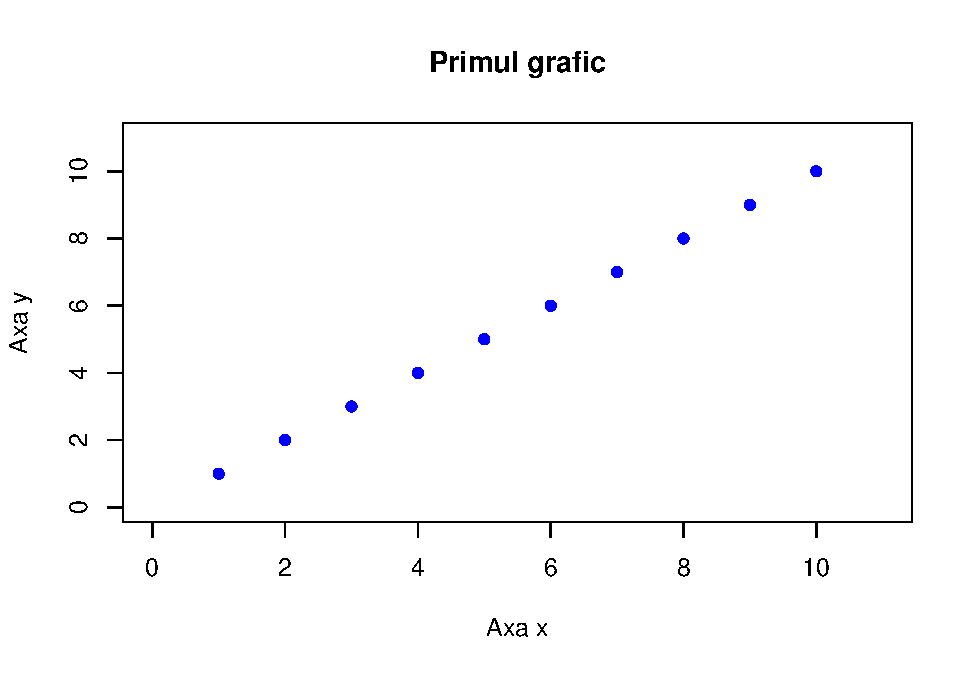
\includegraphics[width=0.8\linewidth]{Lab_1_files/figure-latex/unnamed-chunk-84-1} \end{center}

În afară de vectorii \texttt{x} și \texttt{y} toate celelalte argumente
sunt opționale, dacă nu sunt specificate atunci R-ul folosește valorile
prestabilite. De exemplu dacă nu specificăm limitele \texttt{xlim} și
\texttt{ylim}, R-ul calculează aceste limite astfel încât toate punctele
să fie încadrați în interiorul graficului.

\begin{rmdexercise}
Trasați următoarele diagrame de împrăștiere:

\texttt{x\ \textless{}-\ seq(0,\ 1,\ 0.1);\ plot(x,\ x\ -\ x\ *\ x\ +\ 2)}
\texttt{plot(x,\ x\ -\ x\ *\ x\ +\ 2,\ type\ =\ "l");\ plot(x,\ x\ -\ x\ *\ x\ +\ 2,\ type\ =\ "b",\ pch\ =\ 19)}
\end{rmdexercise}

Tipul de simbol pe care vrem să-l folosim atunci când trasăm un grafic
este specificat prin argumentul \texttt{pch}. Figura de mai jos ne
prezintă tipurile simboluri pe care atunci când atribuim argumentului
\texttt{pch} o valoare întreagă.

\begin{figure}

{\centering 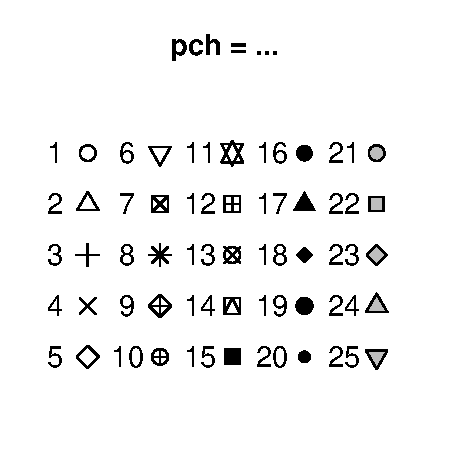
\includegraphics{Lab_1_files/figure-latex/unnamed-chunk-86-1} 

}

\caption{Tipurile de simboluri asociate parametrului pch.}\label{fig:unnamed-chunk-86}
\end{figure}

Următorul exemplu ilustrează câteva tipuri de simboluri:

\begin{center}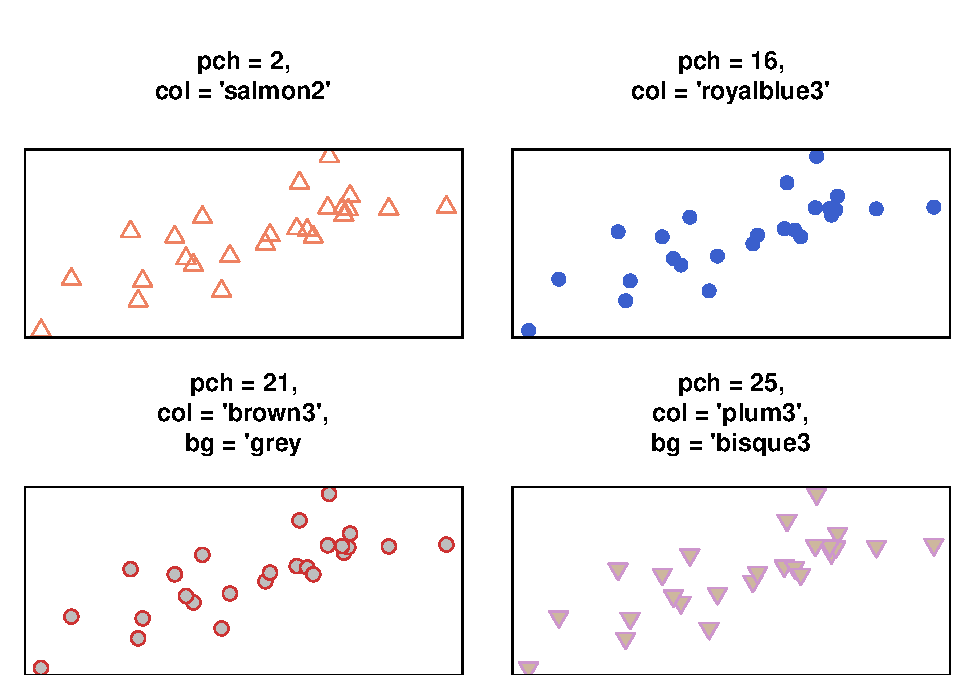
\includegraphics[width=0.8\linewidth]{Lab_1_files/figure-latex/unnamed-chunk-87-1} \end{center}

\begin{rmdexercise}
Considerăm următoarea funcție \(g:\mathbb{R}\to\mathbb{R}\),

\[
  g(x) = \left\{\begin{array}{ll}
              \sin^2(x)\log(x), & x>0\\
              \sin^2(x)x, & x\leq 0
  \end{array}\right.
\]

\begin{enumerate}
\def\labelenumi{\alph{enumi})}
\item
  Definiți funcția folosind comenzile \texttt{if-else} și
  \texttt{Vectorize} iar apoi folosind comanda \texttt{ifelse}.
\item
  Trasați graficul curbei pe intervalul \([-\pi, \pi]\).
\end{enumerate}
\end{rmdexercise}

\subsection{Culori}\label{culori}

Majoritatea funcțiilor de desenare au un argument în care pot specifica
culoarea elementelor pe care vrem să le trasăm, de cele mai multe ori
acesta este \texttt{col}. Cel mai ușor mod de a introduce o culoare este
prin specificarea numelui acesteia, de exemplu
\texttt{col\ =\ \textquotesingle{}red\textquotesingle{}} este culoarea
roșie. Figura 1 prezintă 144 de culori alese la întâmplare din totalul
de 657 câte există în R.

\begin{figure}

{\centering 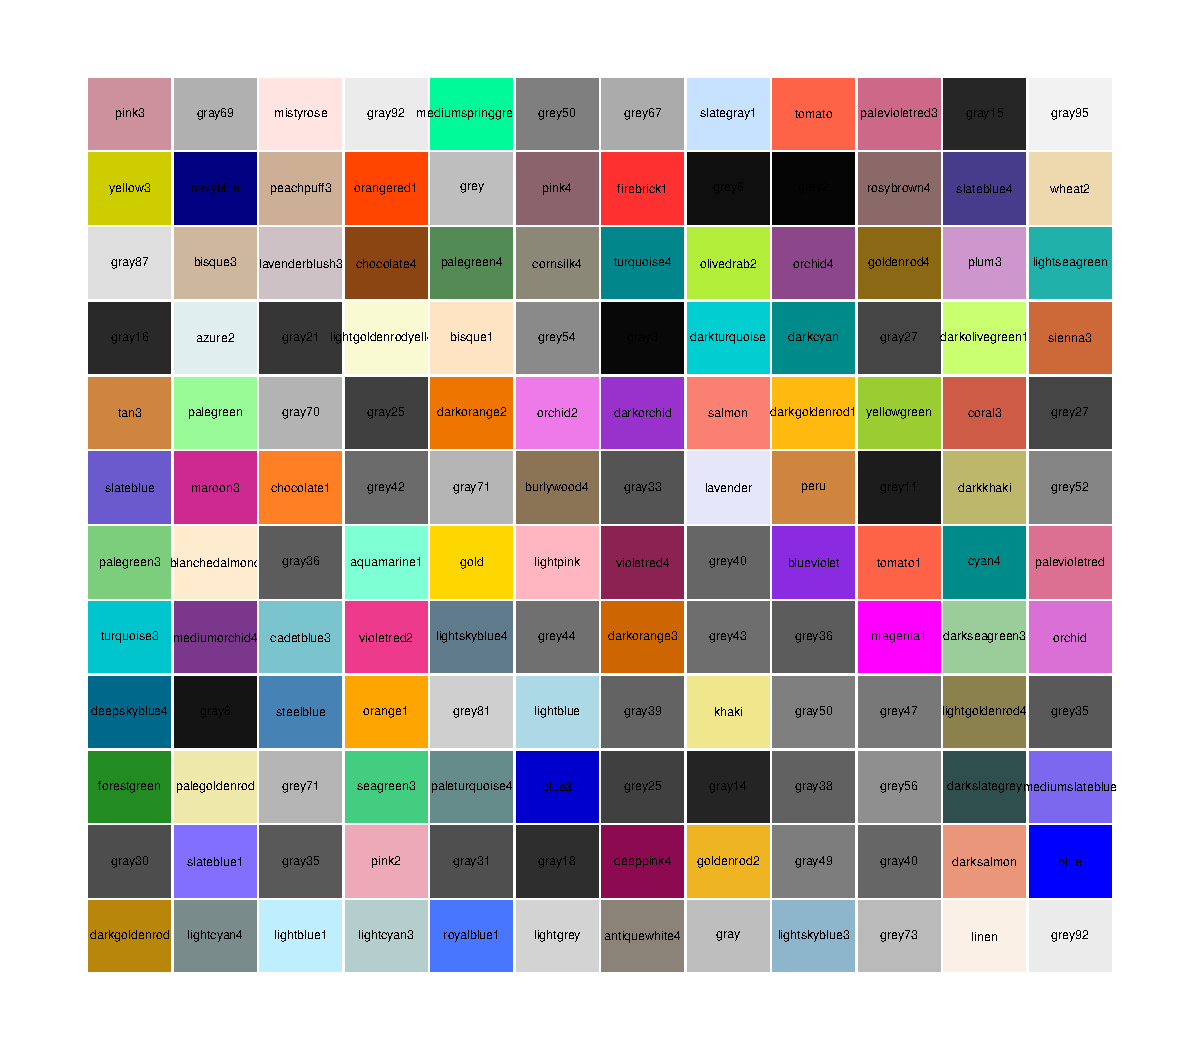
\includegraphics{Lab_1_files/figure-latex/randomcolors-1} 

}

\caption{144 de culori din totalul de 657 din R}\label{fig:randomcolors}
\end{figure}

Pentru a vedea toate culorile din R putem rula comanda
\texttt{colors()}.

\subsection{\texorpdfstring{Funcția
\texttt{hist}}{Funcția hist}}\label{functia-hist}

Histograma\footnote{Histograma este un estimator neparametric al
  densității.} reprezintă metoda grafică, cea mai comună, de
reprezentare a repartiției unui vector numeric. Pentru a crea o
histogramă în R folosim funcția \texttt{hist()} în care argumentul
principal este un vector numeric. Tabelul de mai jos prezintă
argumentele principale ale funcției \texttt{hist}.

\begin{longtable}[]{@{}ll@{}}
\caption{Argumentele funcției \texttt{hist()}}\tabularnewline
\toprule
\begin{minipage}[b]{0.18\columnwidth}\raggedright\strut
Argument\strut
\end{minipage} & \begin{minipage}[b]{0.67\columnwidth}\raggedright\strut
Descriere\strut
\end{minipage}\tabularnewline
\midrule
\endfirsthead
\toprule
\begin{minipage}[b]{0.18\columnwidth}\raggedright\strut
Argument\strut
\end{minipage} & \begin{minipage}[b]{0.67\columnwidth}\raggedright\strut
Descriere\strut
\end{minipage}\tabularnewline
\midrule
\endhead
\begin{minipage}[t]{0.18\columnwidth}\raggedright\strut
\texttt{x}\strut
\end{minipage} & \begin{minipage}[t]{0.67\columnwidth}\raggedright\strut
Vector de valori\strut
\end{minipage}\tabularnewline
\begin{minipage}[t]{0.18\columnwidth}\raggedright\strut
\texttt{breaks}\strut
\end{minipage} & \begin{minipage}[t]{0.67\columnwidth}\raggedright\strut
Cum să calculăm mărimea bin-urilor (vezi \texttt{?hist})\strut
\end{minipage}\tabularnewline
\begin{minipage}[t]{0.18\columnwidth}\raggedright\strut
\texttt{freq}\strut
\end{minipage} & \begin{minipage}[t]{0.67\columnwidth}\raggedright\strut
Opțiune pentru trasarea histogramei de frecvență și de probabilități,
\texttt{freq\ =\ TRUE} arată frecvențele, \texttt{freq\ =\ FALSE} arată
probabilitățile.\strut
\end{minipage}\tabularnewline
\begin{minipage}[t]{0.18\columnwidth}\raggedright\strut
\texttt{col}, \texttt{border}\strut
\end{minipage} & \begin{minipage}[t]{0.67\columnwidth}\raggedright\strut
Culoarea interioară a bin-urilor (\texttt{col}) și culoarea conturului
lor (\texttt{border})\strut
\end{minipage}\tabularnewline
\bottomrule
\end{longtable}

Putem crea o histogramă folosind setul de date \texttt{ChickWeight}
(\texttt{?ChickWeight})

\begin{Shaded}
\begin{Highlighting}[]
\KeywordTok{hist}\NormalTok{(}\DataTypeTok{x =}\NormalTok{ ChickWeight}\OperatorTok{$}\NormalTok{weight,}
     \DataTypeTok{main =} \StringTok{"Histograma greutatii gainilor"}\NormalTok{,}
     \DataTypeTok{xlab =} \StringTok{"Greutate"}\NormalTok{,}
     \DataTypeTok{ylab =} \StringTok{"Frecventa"}\NormalTok{,}
     \DataTypeTok{xlim =} \KeywordTok{c}\NormalTok{(}\DecValTok{0}\NormalTok{, }\DecValTok{500}\NormalTok{))}
\end{Highlighting}
\end{Shaded}

\begin{center}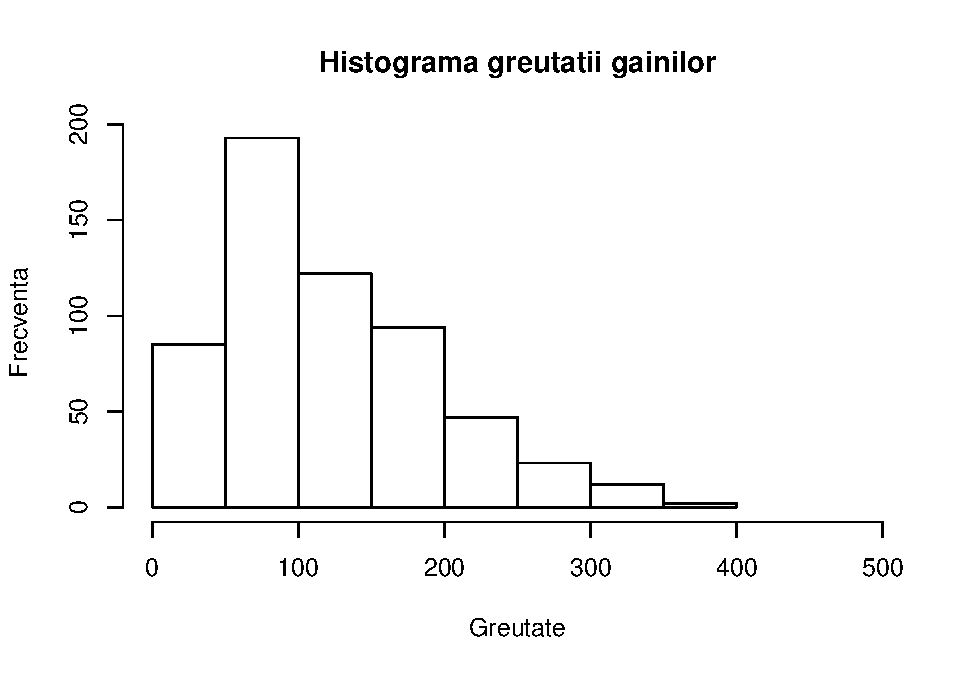
\includegraphics[width=0.8\linewidth]{Lab_1_files/figure-latex/unnamed-chunk-89-1} \end{center}

Putem modifica histograma de mai sus, schimbând numărul de bin-uri și
culoarea acestora:

\begin{Shaded}
\begin{Highlighting}[]
\KeywordTok{hist}\NormalTok{(}\DataTypeTok{x =}\NormalTok{ ChickWeight}\OperatorTok{$}\NormalTok{weight,}
     \DataTypeTok{main =} \StringTok{"O histograma mai colorata"}\NormalTok{,}
     \DataTypeTok{xlab =} \StringTok{"Greutate"}\NormalTok{,}
     \DataTypeTok{ylab =} \StringTok{"Frecventa"}\NormalTok{,}
     \DataTypeTok{breaks =} \DecValTok{20}\NormalTok{, }\CommentTok{# 20 Bins}
     \DataTypeTok{xlim =} \KeywordTok{c}\NormalTok{(}\DecValTok{0}\NormalTok{, }\DecValTok{500}\NormalTok{),}
     \DataTypeTok{col =} \StringTok{"skyblue"}\NormalTok{, }\CommentTok{# Culoarea de umplere}
     \DataTypeTok{border =} \StringTok{"royalblue3"}\NormalTok{) }\CommentTok{# Culoarea conturului}
\end{Highlighting}
\end{Shaded}

\begin{center}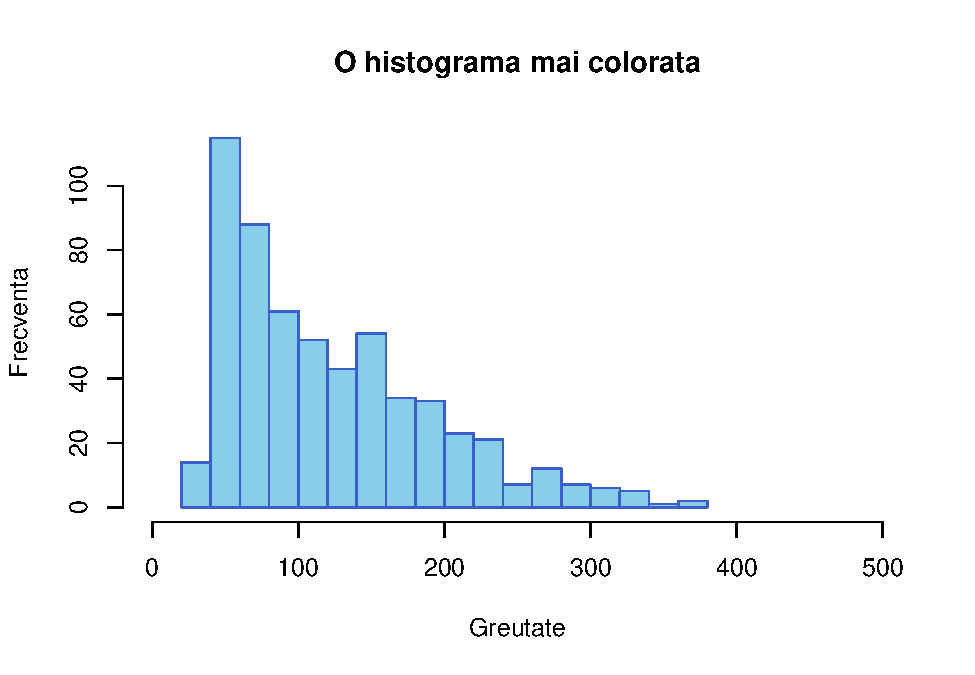
\includegraphics[width=0.8\linewidth]{Lab_1_files/figure-latex/unnamed-chunk-90-1} \end{center}

Dacă vrem să ilustrăm două histograme pe aceeași figură, pentru a
evidenția repartiția după două clase, putem folosi argumentul
\texttt{add\ =\ TRUE} la cel de-al doilea plot:

\begin{Shaded}
\begin{Highlighting}[]
\KeywordTok{hist}\NormalTok{(}\DataTypeTok{x =}\NormalTok{ ChickWeight}\OperatorTok{$}\NormalTok{weight[ChickWeight}\OperatorTok{$}\NormalTok{Diet }\OperatorTok{==}\StringTok{ }\DecValTok{1}\NormalTok{],}
     \DataTypeTok{main =} \StringTok{"Doua histograme pe acelasi grafic"}\NormalTok{,}
     \DataTypeTok{xlab =} \StringTok{"Greutate"}\NormalTok{,}
     \DataTypeTok{ylab =} \StringTok{"Frecventa"}\NormalTok{,}
     \DataTypeTok{breaks =} \DecValTok{20}\NormalTok{,}
     \DataTypeTok{xlim =} \KeywordTok{c}\NormalTok{(}\DecValTok{0}\NormalTok{, }\DecValTok{500}\NormalTok{),}
     \DataTypeTok{col =} \KeywordTok{gray}\NormalTok{(}\DecValTok{0}\NormalTok{, .}\DecValTok{5}\NormalTok{))}

\KeywordTok{hist}\NormalTok{(}\DataTypeTok{x =}\NormalTok{ ChickWeight}\OperatorTok{$}\NormalTok{weight[ChickWeight}\OperatorTok{$}\NormalTok{Diet }\OperatorTok{==}\StringTok{ }\DecValTok{2}\NormalTok{],}
     \DataTypeTok{breaks =} \DecValTok{30}\NormalTok{,}
     \DataTypeTok{add =} \OtherTok{TRUE}\NormalTok{, }\CommentTok{# Adauga graficul la cel de dinainte}
     \DataTypeTok{col =} \KeywordTok{gray}\NormalTok{(}\DecValTok{1}\NormalTok{, .}\DecValTok{8}\NormalTok{))}
\end{Highlighting}
\end{Shaded}

\begin{center}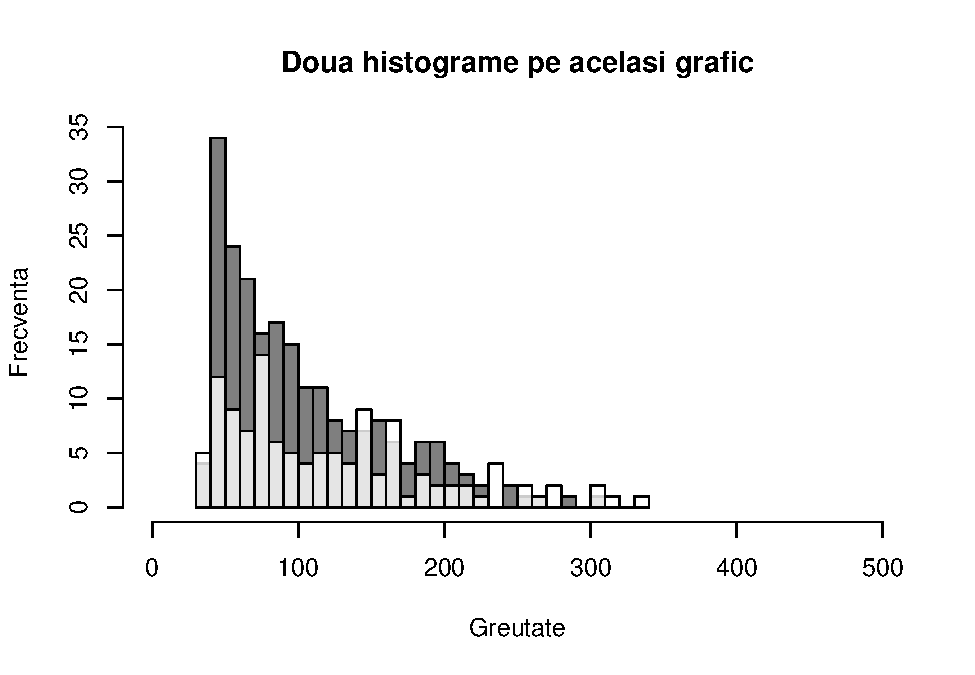
\includegraphics[width=0.8\linewidth]{Lab_1_files/figure-latex/unnamed-chunk-91-1} \end{center}

\subsection{\texorpdfstring{Funcția
\texttt{barplot}}{Funcția barplot}}\label{functia-barplot}

Funcția \texttt{barplot} este folosită în special atunci când avem de-a
face cu o variabilă discretă. Argumentul principal al funcției este
\texttt{height}, un vector numeric care va genera înălțimea fiecărei
bare. Pentru a adăuga nume sub fiecare bară putem folosi argumentul
\texttt{names.arg}.

De exemplu, folosind setul de date \texttt{mtcars} putem să afișăm
greutatea medie a mașinilor în funcție de numărul de cilindrii:

\begin{Shaded}
\begin{Highlighting}[]
\KeywordTok{par}\NormalTok{(}\DataTypeTok{mfrow =} \KeywordTok{c}\NormalTok{(}\DecValTok{1}\NormalTok{, }\DecValTok{2}\NormalTok{))}

\NormalTok{weight_cars =}\StringTok{ }\KeywordTok{aggregate}\NormalTok{(wt }\OperatorTok{~}\StringTok{ }\NormalTok{cyl, }
                        \DataTypeTok{data =}\NormalTok{ mtcars, }
                        \DataTypeTok{FUN =}\NormalTok{ mean)}

\KeywordTok{barplot}\NormalTok{(}\DataTypeTok{height =}\NormalTok{ weight_cars}\OperatorTok{$}\NormalTok{wt,}
        \DataTypeTok{names.arg =}\NormalTok{ weight_cars}\OperatorTok{$}\NormalTok{cyl,}
        \DataTypeTok{xlab =} \StringTok{"Numar de cilindrii"}\NormalTok{,}
        \DataTypeTok{ylab =} \StringTok{"Greutatea medie"}\NormalTok{,}
        \DataTypeTok{main =} \StringTok{"Greutatea medie dupa numarul de cilindrii}\CharTok{\textbackslash{}n}\StringTok{ Barplot vertical"}\NormalTok{,}
        \DataTypeTok{col =} \StringTok{"grey80"}\NormalTok{, }
        \DataTypeTok{cex.main =} \FloatTok{0.7}\NormalTok{)}

\KeywordTok{barplot}\NormalTok{(}\DataTypeTok{height =}\NormalTok{ weight_cars}\OperatorTok{$}\NormalTok{wt,}
        \DataTypeTok{names.arg =}\NormalTok{ weight_cars}\OperatorTok{$}\NormalTok{cyl,}
        \DataTypeTok{horiz =} \OtherTok{TRUE}\NormalTok{,}
        \DataTypeTok{ylab =} \StringTok{"Numar de cilindrii"}\NormalTok{,}
        \DataTypeTok{xlab =} \StringTok{"Greutatea medie"}\NormalTok{,}
        \DataTypeTok{main =} \StringTok{"Greutatea medie dupa numarul de cilindrii}\CharTok{\textbackslash{}n}\StringTok{ Barplot orizontal"}\NormalTok{,}
        \DataTypeTok{col =} \StringTok{"grey80"}\NormalTok{, }
        \DataTypeTok{cex.main =} \FloatTok{0.7}\NormalTok{)}
\end{Highlighting}
\end{Shaded}

\begin{center}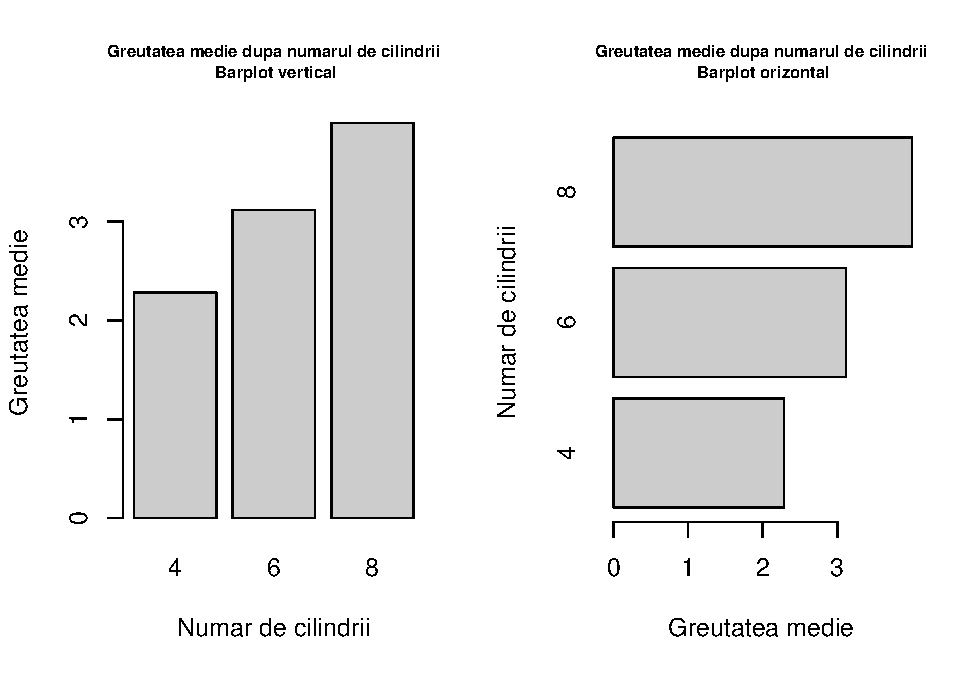
\includegraphics[width=0.8\linewidth]{Lab_1_files/figure-latex/unnamed-chunk-92-1} \end{center}

\begin{rmdexercise}
Folosind setul de date \texttt{ChickWeight} afișați, cu ajutorul
funcției \texttt{barplot}, greutatea medie a găinilor în raport cu
numărul de zile de la naștere.
\end{rmdexercise}

De asemenea putem crea un barplot clusterizat în funcție de mai multe
grupuri de date. De exemplu să presupunem că vrem să vedem dacă există
diferențe între greutatea medie a mașinilor (din setul de date
\texttt{mtcars}) care au transmisie manuală sau automată și numărul de
cilindrii.

\begin{Shaded}
\begin{Highlighting}[]
\CommentTok{# calculam greutatea medie dupa numarul de cilindrii si transmisie }
\NormalTok{carWeight_cyl_am =}\StringTok{ }\KeywordTok{aggregate}\NormalTok{(mtcars}\OperatorTok{$}\NormalTok{wt, }\DataTypeTok{by =} \KeywordTok{list}\NormalTok{(mtcars}\OperatorTok{$}\NormalTok{cyl, mtcars}\OperatorTok{$}\NormalTok{am), }\DataTypeTok{FUN =}\NormalTok{ mean) }

\CommentTok{# transformam rezultatul sub forma de matrice}
\NormalTok{carWeight_cyl_am =}\StringTok{ }\KeywordTok{as.matrix}\NormalTok{(carWeight_cyl_am)}
\NormalTok{carWeight_cyl_am}
\NormalTok{     Group.}\DecValTok{1}\NormalTok{ Group.}\DecValTok{2}\NormalTok{        x}
\NormalTok{[}\DecValTok{1}\NormalTok{,]       }\DecValTok{4}       \DecValTok{0} \FloatTok{2.935000}
\NormalTok{[}\DecValTok{2}\NormalTok{,]       }\DecValTok{6}       \DecValTok{0} \FloatTok{3.388750}
\NormalTok{[}\DecValTok{3}\NormalTok{,]       }\DecValTok{8}       \DecValTok{0} \FloatTok{4.104083}
\NormalTok{[}\DecValTok{4}\NormalTok{,]       }\DecValTok{4}       \DecValTok{1} \FloatTok{2.042250}
\NormalTok{[}\DecValTok{5}\NormalTok{,]       }\DecValTok{6}       \DecValTok{1} \FloatTok{2.755000}
\NormalTok{[}\DecValTok{6}\NormalTok{,]       }\DecValTok{8}       \DecValTok{1} \FloatTok{3.370000}

\CommentTok{# aducem la forma necesara pentru barplot}
\NormalTok{carWeight =}\StringTok{ }\KeywordTok{matrix}\NormalTok{(carWeight_cyl_am[,}\DecValTok{3}\NormalTok{], }\DataTypeTok{nrow =} \DecValTok{3}\NormalTok{)}
\KeywordTok{colnames}\NormalTok{(carWeight) =}\StringTok{ }\KeywordTok{unique}\NormalTok{(carWeight_cyl_am[,}\DecValTok{2}\NormalTok{])}
\KeywordTok{rownames}\NormalTok{(carWeight) =}\StringTok{ }\KeywordTok{unique}\NormalTok{(carWeight_cyl_am[, }\DecValTok{1}\NormalTok{])}

\NormalTok{carWeight =}\StringTok{ }\KeywordTok{t}\NormalTok{(carWeight)}

\KeywordTok{barplot}\NormalTok{(carWeight, }
        \DataTypeTok{beside =} \OtherTok{TRUE}\NormalTok{,}
        \DataTypeTok{legend.text =} \OtherTok{TRUE}\NormalTok{, }
        \DataTypeTok{col =} \KeywordTok{c}\NormalTok{(}\StringTok{"royalblue3"}\NormalTok{, }\StringTok{"brown3"}\NormalTok{),}
        \DataTypeTok{main =} \StringTok{"Greutatea medie a masinilor dupa numarul de cilindrii si transmisie"}\NormalTok{,}
        \DataTypeTok{xlab =} \StringTok{"Numar de cilindrii"}\NormalTok{,}
        \DataTypeTok{ylab =} \StringTok{"Greutatea medie"}\NormalTok{)}
\end{Highlighting}
\end{Shaded}

\begin{center}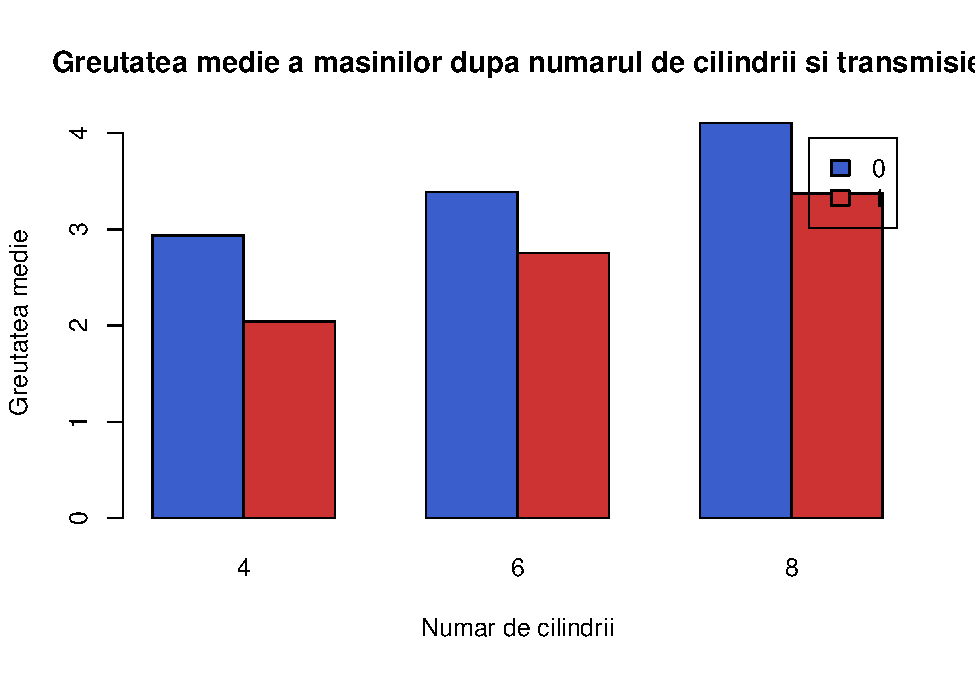
\includegraphics[width=0.8\linewidth]{Lab_1_files/figure-latex/unnamed-chunk-94-1} \end{center}

\subsection{\texorpdfstring{Funcția
\texttt{boxplot}}{Funcția boxplot}}\label{functia-boxplot}

Pentru a vedea cât de bine sunt repartizate datele în setul de date
putem folosi funcția \texttt{boxplot} (box and whisker plot - cutie cu
mustăți). Această funcție prezintă într-o manieră compactă modul în care
este repartizată o variabilă. Această metodă grafică prezintă
principalii indicatori de poziție ai variabilei studiate: cuartilele de
ordin 1 și 3 (\(Q_1\), \(Q_3\)) care delimitează cutia
(\(IQR = Q_3-Q_1\)) și cuartila de ordin 2 sau mediana (linia din
interiorul cutiei). Mustățile sunt calculate în modul următor: mustața
superioară este determinată de valoarea celei mai mari observații care
este mai mică sau egală cu \(Q_3 + 1.5 IQR\) iar mustața inferioară este
valoarea celei mai mici observații mai mari sau egale cu \(Q_1-1.5IQR\).
Valorile din afara cutiei cu mustăți se numesc valori aberante.

Principalele argumente ale funcției \texttt{boxplot} se regăsesc în
tabelul următor, pentru mai multe detalii apelați \texttt{?boxplot}.

\begin{longtable}[]{@{}ll@{}}
\caption{Principalele argumente ale functiei boxplot.}\tabularnewline
\toprule
\begin{minipage}[b]{0.18\columnwidth}\raggedright\strut
Argument\strut
\end{minipage} & \begin{minipage}[b]{0.67\columnwidth}\raggedright\strut
Descriere\strut
\end{minipage}\tabularnewline
\midrule
\endfirsthead
\toprule
\begin{minipage}[b]{0.18\columnwidth}\raggedright\strut
Argument\strut
\end{minipage} & \begin{minipage}[b]{0.67\columnwidth}\raggedright\strut
Descriere\strut
\end{minipage}\tabularnewline
\midrule
\endhead
\begin{minipage}[t]{0.18\columnwidth}\raggedright\strut
\texttt{formula}\strut
\end{minipage} & \begin{minipage}[t]{0.67\columnwidth}\raggedright\strut
O formulă de tip \texttt{y\ \textasciitilde{}\ grp}, unde \texttt{y}
este variabila investigată iar \texttt{grp} este variabila care descrie
grupurile după care vrem să trasăm grafiul\strut
\end{minipage}\tabularnewline
\begin{minipage}[t]{0.18\columnwidth}\raggedright\strut
\texttt{data}\strut
\end{minipage} & \begin{minipage}[t]{0.67\columnwidth}\raggedright\strut
Un data frame (sau listă) în care variabilele din formulă sunt
definite\strut
\end{minipage}\tabularnewline
\begin{minipage}[t]{0.18\columnwidth}\raggedright\strut
\texttt{subset}\strut
\end{minipage} & \begin{minipage}[t]{0.67\columnwidth}\raggedright\strut
Un vector care specifică o submulțime a observațiilor\strut
\end{minipage}\tabularnewline
\begin{minipage}[t]{0.18\columnwidth}\raggedright\strut
\texttt{x}\strut
\end{minipage} & \begin{minipage}[t]{0.67\columnwidth}\raggedright\strut
Un vector care specifică valorile ce urmează să fie trasate\strut
\end{minipage}\tabularnewline
\begin{minipage}[t]{0.18\columnwidth}\raggedright\strut
\texttt{horizontal}\strut
\end{minipage} & \begin{minipage}[t]{0.67\columnwidth}\raggedright\strut
O valoare logică care indică dacă trasăm boxplot-urile vertical
(\texttt{FALSE}) sau orizontal (\texttt{TRUE})\strut
\end{minipage}\tabularnewline
\begin{minipage}[t]{0.18\columnwidth}\raggedright\strut
\texttt{add}\strut
\end{minipage} & \begin{minipage}[t]{0.67\columnwidth}\raggedright\strut
O valoare logică prin care se permite adăugarea graficului la unul deja
existent\strut
\end{minipage}\tabularnewline
\bottomrule
\end{longtable}

Următorul exemplu ne prezintă relația dintre consum (\texttt{mpg}) și
numărul de cilindrii (\texttt{cyl}) în cazul mașinilor din setul de date
\texttt{mtcars}.

\begin{Shaded}
\begin{Highlighting}[]
\KeywordTok{boxplot}\NormalTok{(mpg }\OperatorTok{~}\StringTok{ }\NormalTok{cyl, }
        \DataTypeTok{data =}\NormalTok{ mtcars, }
        \DataTypeTok{xlab =} \StringTok{"Numar de cilindrii"}\NormalTok{,}
        \DataTypeTok{ylab =} \StringTok{"Mile pe galon"}\NormalTok{, }
        \DataTypeTok{main =} \StringTok{"Consumul in functie de numarul de cilindrii"}\NormalTok{)}
\end{Highlighting}
\end{Shaded}

\begin{center}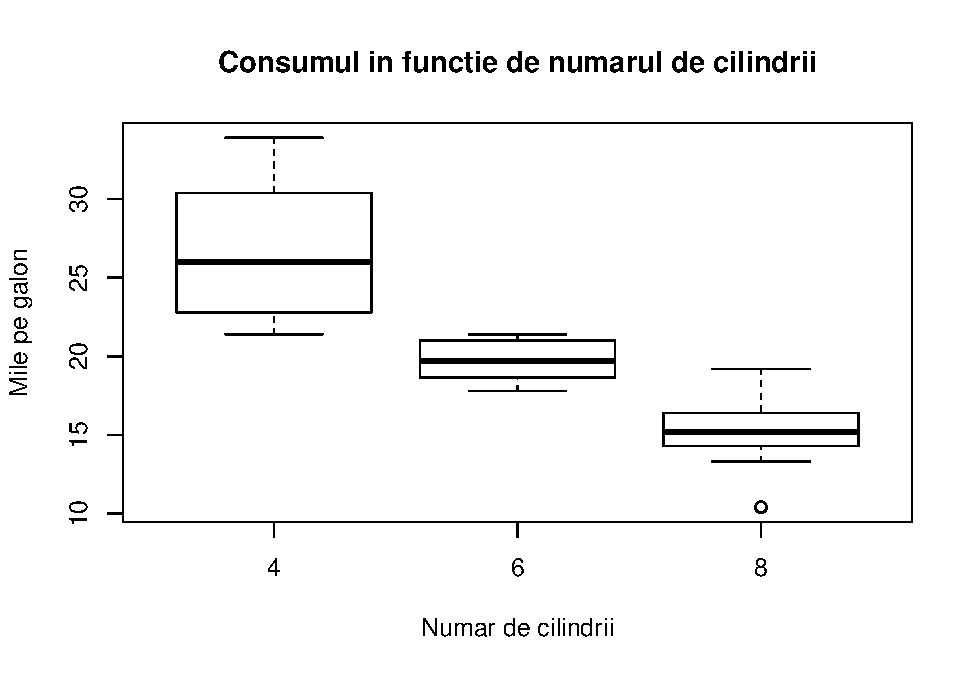
\includegraphics[width=0.8\linewidth]{Lab_1_files/figure-latex/unnamed-chunk-95-1} \end{center}

Putem să vedem această relație și în raport cu tipul de transmisie.

\begin{Shaded}
\begin{Highlighting}[]
\KeywordTok{boxplot}\NormalTok{(mpg }\OperatorTok{~}\StringTok{ }\NormalTok{cyl, }
        \DataTypeTok{data =}\NormalTok{ mtcars, }
        \DataTypeTok{subset =}\NormalTok{ am }\OperatorTok{==}\StringTok{ }\DecValTok{0}\NormalTok{,}
        \DataTypeTok{boxwex =} \FloatTok{0.25}\NormalTok{, }
        \DataTypeTok{at =} \DecValTok{1}\OperatorTok{:}\DecValTok{3} \OperatorTok{-}\StringTok{ }\FloatTok{0.2}\NormalTok{,}
        \DataTypeTok{col =} \StringTok{"darkgrey"}\NormalTok{,}
        \DataTypeTok{xlab =} \StringTok{"Numar de cilindrii"}\NormalTok{,}
        \DataTypeTok{ylab =} \StringTok{"Mile pe galon"}\NormalTok{, }
        \DataTypeTok{main =} \StringTok{"Consumul dupa de numarul de cilindrii si transmisie"}\NormalTok{,}
        \DataTypeTok{xlim =} \KeywordTok{c}\NormalTok{(}\FloatTok{0.5}\NormalTok{, }\FloatTok{3.5}\NormalTok{), }
        \DataTypeTok{ylim =} \KeywordTok{c}\NormalTok{(}\DecValTok{0}\NormalTok{, }\DecValTok{35}\NormalTok{),}
        \DataTypeTok{yaxs =} \StringTok{"i"}\NormalTok{)}

\KeywordTok{boxplot}\NormalTok{(mpg }\OperatorTok{~}\StringTok{ }\NormalTok{cyl, }
        \DataTypeTok{data =}\NormalTok{ mtcars, }
        \DataTypeTok{subset =}\NormalTok{ am }\OperatorTok{==}\StringTok{ }\DecValTok{1}\NormalTok{,}
        \DataTypeTok{add =} \OtherTok{TRUE}\NormalTok{,}
        \DataTypeTok{boxwex =} \FloatTok{0.25}\NormalTok{, }
        \DataTypeTok{at =} \DecValTok{1}\OperatorTok{:}\DecValTok{3} \OperatorTok{+}\StringTok{ }\FloatTok{0.2}\NormalTok{,}
        \DataTypeTok{col =} \StringTok{"brown3"}\NormalTok{)}

\KeywordTok{legend}\NormalTok{(}\StringTok{"bottomright"}\NormalTok{ ,}\KeywordTok{c}\NormalTok{(}\StringTok{"Manuala"}\NormalTok{, }\StringTok{"Automata"}\NormalTok{),}
       \DataTypeTok{fill =} \KeywordTok{c}\NormalTok{(}\StringTok{"lightgray"}\NormalTok{, }\StringTok{"brown3"}\NormalTok{), }\DataTypeTok{bty =} \StringTok{"n"}\NormalTok{)}
\end{Highlighting}
\end{Shaded}

\begin{center}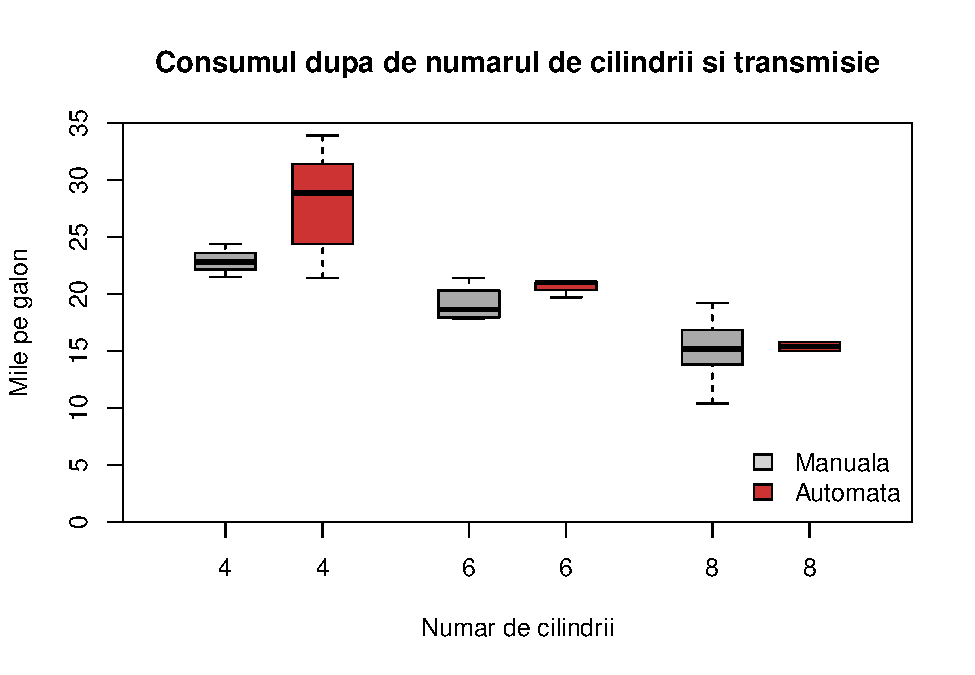
\includegraphics[width=0.8\linewidth]{Lab_1_files/figure-latex/unnamed-chunk-96-1} \end{center}

\subsection{Funcții pentru adăugarea unor elemente la un
grafic}\label{functii-pentru-adaugarea-unor-elemente-la-un-grafic}

Funcțiile (low-level) din această secțiune sunt folosite pentru a adăuga
elemente, de tipul linii, puncte, text la un grafic deja existent.

\begin{longtable}[]{@{}ll@{}}
\caption{Functii low-level uzuale}\tabularnewline
\toprule
Funcția & rezultatul\tabularnewline
\midrule
\endfirsthead
\toprule
Funcția & rezultatul\tabularnewline
\midrule
\endhead
\texttt{points(x,\ y)} & Adaugă puncte la un grafic.\tabularnewline
\texttt{abline()}, \texttt{segments()} & Adaugă linii sau segmente la un
grafic existent.\tabularnewline
\texttt{arrows()} & Adaugă săgeți.\tabularnewline
\texttt{curve()} & Adaugă o curbă care reprezintă graficul unei
funcții.\tabularnewline
\texttt{rect()},\texttt{polygon()} & Adaugă un dreptunghi sau un poligon
oarecare.\tabularnewline
\texttt{text()}, \texttt{mtext()} & Adaugă text la o
figură.\tabularnewline
\texttt{legend()} & Adaugă legenda.\tabularnewline
\texttt{axis()} & Adaugă o axă.\tabularnewline
\bottomrule
\end{longtable}

Pentru a adăuga noi puncte la un grafic deja existent putem folosi
funcție \texttt{points()}. Pentru a vedea toate argumentele acestei
funcții apelați \texttt{?points}.

Să considerăm următorul exemplu în care trasăm diagrama de împrăștiere
după consum (\texttt{mpg}) și putere (\texttt{hp}) pentru mașinile din
setul de date \texttt{mtcars} în raport cu tipul de transmisie.

\begin{Shaded}
\begin{Highlighting}[]
\KeywordTok{plot}\NormalTok{(}\DataTypeTok{x =}\NormalTok{ mtcars}\OperatorTok{$}\NormalTok{mpg[mtcars}\OperatorTok{$}\NormalTok{am }\OperatorTok{==}\StringTok{ }\DecValTok{0}\NormalTok{], }
     \DataTypeTok{y =}\NormalTok{ mtcars}\OperatorTok{$}\NormalTok{hp[mtcars}\OperatorTok{$}\NormalTok{am }\OperatorTok{==}\StringTok{ }\DecValTok{0}\NormalTok{], }
     \DataTypeTok{xlab =} \StringTok{"Mile pe galon"}\NormalTok{,}
     \DataTypeTok{ylab =} \StringTok{"Cai putere"}\NormalTok{, }
     \DataTypeTok{main =} \StringTok{"Consum vs Cai putere dupa transmisie"}\NormalTok{,}
     \DataTypeTok{pch =} \DecValTok{16}\NormalTok{, }
     \DataTypeTok{col =} \StringTok{"darkgrey"}\NormalTok{)}

\KeywordTok{points}\NormalTok{(}\DataTypeTok{x =}\NormalTok{ mtcars}\OperatorTok{$}\NormalTok{mpg[mtcars}\OperatorTok{$}\NormalTok{am }\OperatorTok{==}\StringTok{ }\DecValTok{1}\NormalTok{], }
      \DataTypeTok{y =}\NormalTok{ mtcars}\OperatorTok{$}\NormalTok{hp[mtcars}\OperatorTok{$}\NormalTok{am }\OperatorTok{==}\StringTok{ }\DecValTok{1}\NormalTok{], }
      \DataTypeTok{pch =} \DecValTok{16}\NormalTok{, }
      \DataTypeTok{col =} \StringTok{"brown3"}\NormalTok{)}
\end{Highlighting}
\end{Shaded}

\begin{center}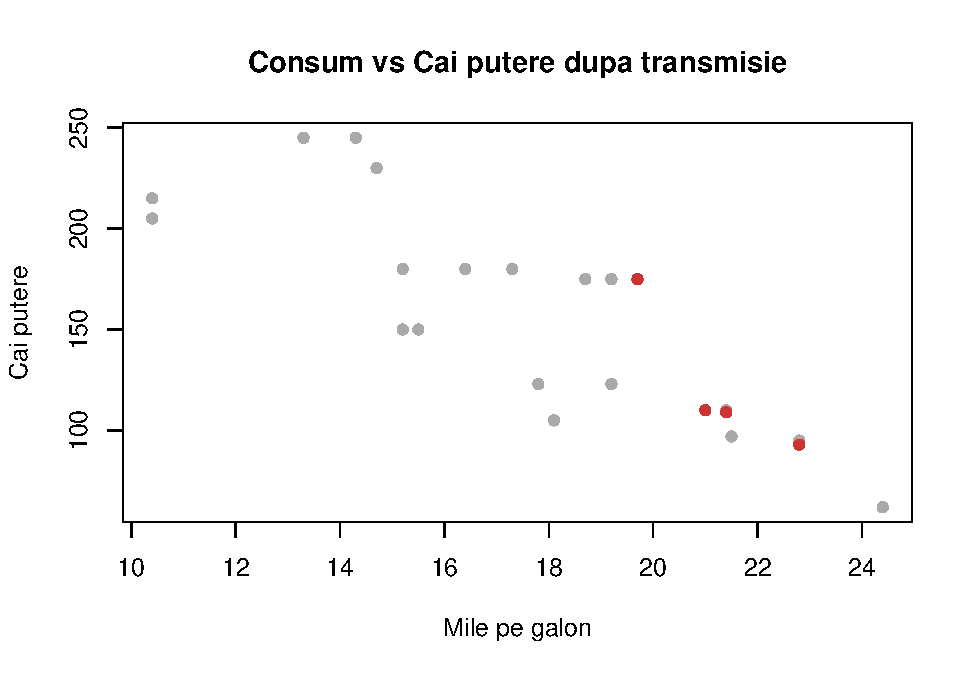
\includegraphics[width=0.8\linewidth]{Lab_1_files/figure-latex/unnamed-chunk-97-1} \end{center}

Dacă vrem să adăugăm linii drepte la un grafic putem folosi comanda
\texttt{abline()} sau \texttt{segments()}. De exemplu în figura de mai
sus vrem să adăugăm o linie verticală și una orizontală care să marcheze
media variabilelor de pe axa x și y.

\begin{Shaded}
\begin{Highlighting}[]
\KeywordTok{plot}\NormalTok{(}\DataTypeTok{x =}\NormalTok{ mtcars}\OperatorTok{$}\NormalTok{mpg, }
     \DataTypeTok{y =}\NormalTok{ mtcars}\OperatorTok{$}\NormalTok{hp, }
     \DataTypeTok{xlab =} \StringTok{"Mile pe galon"}\NormalTok{,}
     \DataTypeTok{ylab =} \StringTok{"Cai putere"}\NormalTok{, }
     \DataTypeTok{main =} \StringTok{"Consum vs Cai putere"}\NormalTok{,}
     \DataTypeTok{pch =} \DecValTok{16}\NormalTok{, }
     \DataTypeTok{col =} \StringTok{"darkgrey"}\NormalTok{)}

\KeywordTok{abline}\NormalTok{(}\DataTypeTok{h =} \KeywordTok{mean}\NormalTok{(mtcars}\OperatorTok{$}\NormalTok{hp), }\DataTypeTok{lty =} \DecValTok{2}\NormalTok{)}
\KeywordTok{abline}\NormalTok{(}\DataTypeTok{v =} \KeywordTok{mean}\NormalTok{(mtcars}\OperatorTok{$}\NormalTok{mpg), }\DataTypeTok{lty =} \DecValTok{2}\NormalTok{)}
\end{Highlighting}
\end{Shaded}

\begin{center}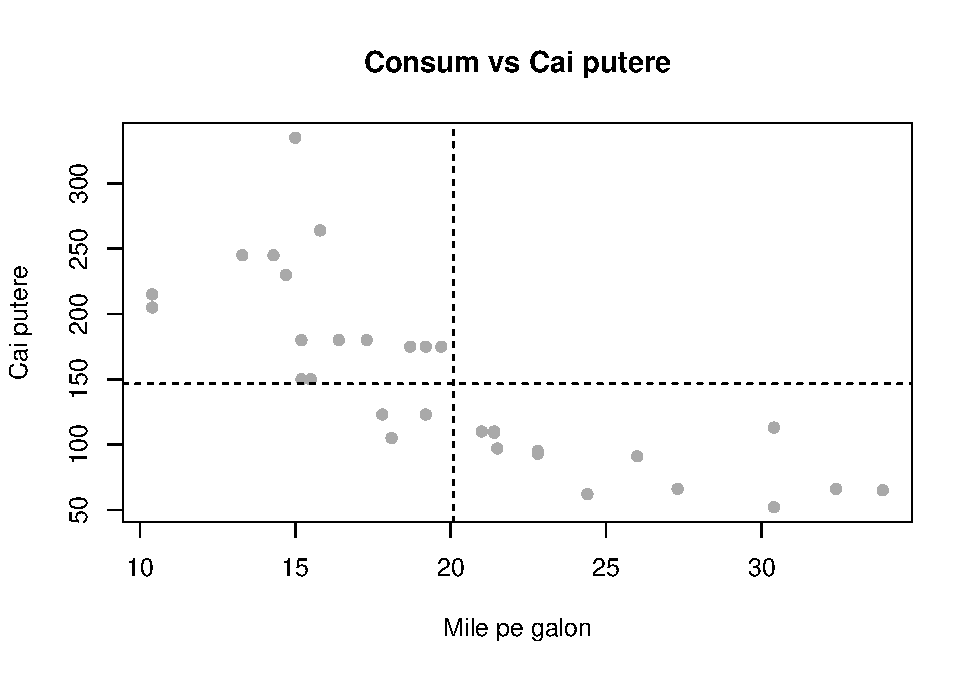
\includegraphics[width=0.8\linewidth]{Lab_1_files/figure-latex/unnamed-chunk-98-1} \end{center}

Pentru a adăuga numele mașinilor cu transmisie automată în fiecare punct
putem folosi comanda \texttt{text()}. Argumentele principale ale acestei
funcții sunt \texttt{x}, \texttt{y} care descriu coordonatele
etichetelor și \texttt{labels} care reprezintă etichetele.

\begin{Shaded}
\begin{Highlighting}[]
\KeywordTok{plot}\NormalTok{(}\DataTypeTok{x =}\NormalTok{ mtcars}\OperatorTok{$}\NormalTok{mpg, }
     \DataTypeTok{y =}\NormalTok{ mtcars}\OperatorTok{$}\NormalTok{hp, }
     \DataTypeTok{xlab =} \StringTok{"Mile pe galon"}\NormalTok{,}
     \DataTypeTok{ylab =} \StringTok{"Cai putere"}\NormalTok{, }
     \DataTypeTok{main =} \StringTok{"Consum vs Cai putere"}\NormalTok{,}
     \DataTypeTok{pch =} \DecValTok{16}\NormalTok{, }
     \DataTypeTok{col =} \StringTok{"darkgrey"}\NormalTok{)}

\KeywordTok{abline}\NormalTok{(}\DataTypeTok{h =} \KeywordTok{mean}\NormalTok{(mtcars}\OperatorTok{$}\NormalTok{hp), }\DataTypeTok{lty =} \DecValTok{2}\NormalTok{)}
\KeywordTok{abline}\NormalTok{(}\DataTypeTok{v =} \KeywordTok{mean}\NormalTok{(mtcars}\OperatorTok{$}\NormalTok{mpg), }\DataTypeTok{lty =} \DecValTok{2}\NormalTok{)}

\KeywordTok{text}\NormalTok{(}\DataTypeTok{x =}\NormalTok{ mtcars}\OperatorTok{$}\NormalTok{mpg[mtcars}\OperatorTok{$}\NormalTok{am }\OperatorTok{==}\StringTok{ }\DecValTok{1}\NormalTok{], }
     \DataTypeTok{y =}\NormalTok{ mtcars}\OperatorTok{$}\NormalTok{hp[mtcars}\OperatorTok{$}\NormalTok{am }\OperatorTok{==}\StringTok{ }\DecValTok{1}\NormalTok{],}
     \DataTypeTok{labels =} \KeywordTok{rownames}\NormalTok{(mtcars[mtcars}\OperatorTok{$}\NormalTok{am }\OperatorTok{==}\StringTok{ }\DecValTok{1}\NormalTok{, ]), }
     \DataTypeTok{pos =} \DecValTok{3}\NormalTok{, }
     \DataTypeTok{cex =} \FloatTok{0.5}\NormalTok{)}
\end{Highlighting}
\end{Shaded}

\begin{center}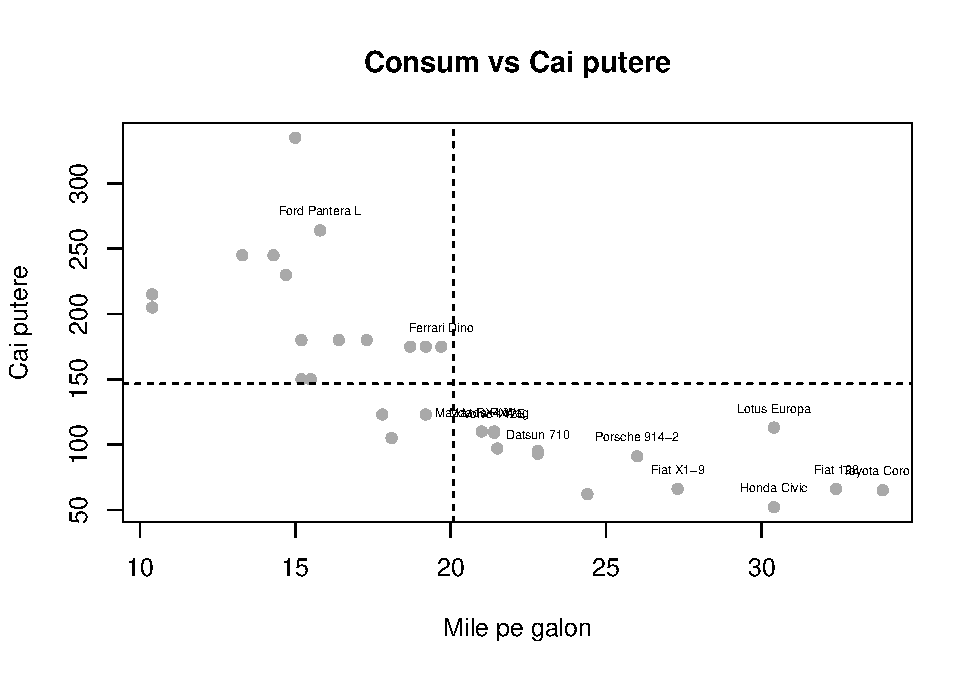
\includegraphics[width=0.8\linewidth]{Lab_1_files/figure-latex/unnamed-chunk-99-1} \end{center}

Funcția \texttt{curve()} permite trasarea/adăugarea unei linii care
descrie o funcție. Printre argumentele funcției regăsim \texttt{expr}
care reprezintă expresia funcției care depinde de \texttt{x} (se pot
folosi și funcții customizate), \texttt{from,\ to} care reprezintă
intervalul de valori pentru \texttt{x} și \texttt{add} care permite
adăugarea unei curbe la un grafic existent.

\begin{Shaded}
\begin{Highlighting}[]
\KeywordTok{curve}\NormalTok{(}\DataTypeTok{expr =} \KeywordTok{sin}\NormalTok{(x),}
      \DataTypeTok{from =} \DecValTok{0}\NormalTok{,}
      \DataTypeTok{to =} \DecValTok{2}\OperatorTok{*}\NormalTok{pi, }
      \DataTypeTok{ylab =} \StringTok{""}\NormalTok{, }
      \DataTypeTok{main =} \StringTok{"Graficul functiei sin si cos"}\NormalTok{,}
      \DataTypeTok{col =} \StringTok{"red"}\NormalTok{)}

\KeywordTok{curve}\NormalTok{(}\DataTypeTok{expr =} \KeywordTok{cos}\NormalTok{(x),}
      \DataTypeTok{from =} \DecValTok{0}\NormalTok{,}
      \DataTypeTok{to =} \DecValTok{2}\OperatorTok{*}\NormalTok{pi,}
      \DataTypeTok{add =} \OtherTok{TRUE}\NormalTok{,}
      \DataTypeTok{col =} \StringTok{"blue"}\NormalTok{, }
      \DataTypeTok{lty =} \DecValTok{2}\NormalTok{)}
\end{Highlighting}
\end{Shaded}

\begin{center}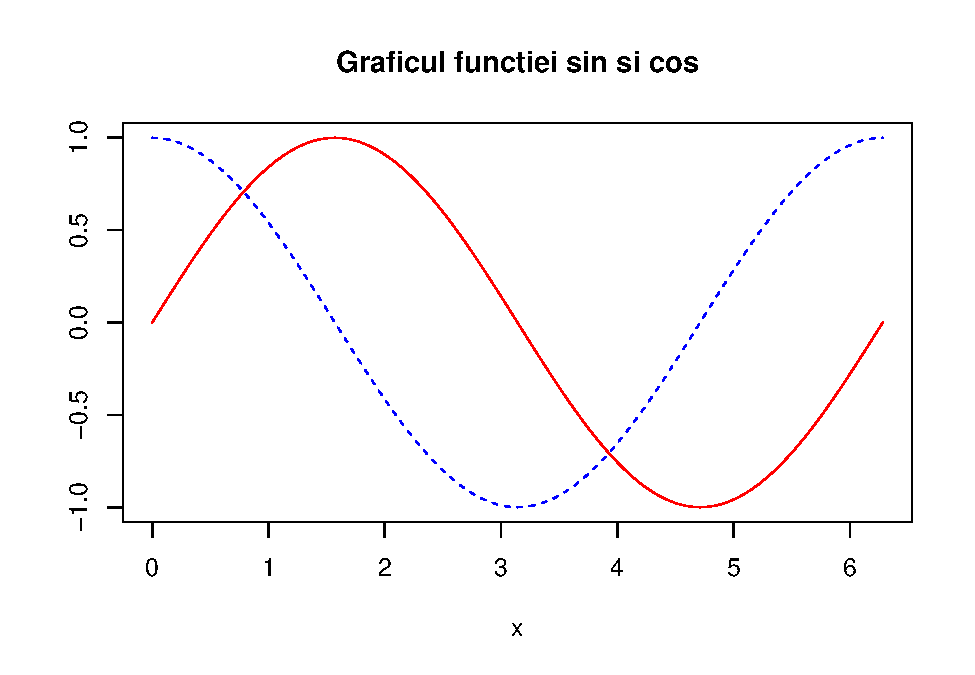
\includegraphics[width=0.8\linewidth]{Lab_1_files/figure-latex/unnamed-chunk-100-1} \end{center}

Atunci când vrem să adăugăm o legendă la un grafic folosim funcția
\texttt{legend()}. Argumentele acestei funcții se regăsesc în tabelul de
mai jos.

\begin{longtable}[]{@{}ll@{}}
\caption{Argumentele functiei legend()}\tabularnewline
\toprule
\begin{minipage}[b]{0.14\columnwidth}\raggedright\strut
Argument\strut
\end{minipage} & \begin{minipage}[b]{0.71\columnwidth}\raggedright\strut
Rezultat\strut
\end{minipage}\tabularnewline
\midrule
\endfirsthead
\toprule
\begin{minipage}[b]{0.14\columnwidth}\raggedright\strut
Argument\strut
\end{minipage} & \begin{minipage}[b]{0.71\columnwidth}\raggedright\strut
Rezultat\strut
\end{minipage}\tabularnewline
\midrule
\endhead
\begin{minipage}[t]{0.14\columnwidth}\raggedright\strut
\texttt{x,\ y}\strut
\end{minipage} & \begin{minipage}[t]{0.71\columnwidth}\raggedright\strut
Coordonatele legendei - de exemplu, \texttt{x\ =\ 0,\ y\ =\ 0} va pune
legenda la coordonatele (0, 0). Alternativ, putem indica poziția unde
vrem legenda (i.e. \texttt{"topright"}, \texttt{"topleft"}).\strut
\end{minipage}\tabularnewline
\begin{minipage}[t]{0.14\columnwidth}\raggedright\strut
\texttt{legend}\strut
\end{minipage} & \begin{minipage}[t]{0.71\columnwidth}\raggedright\strut
Un vector de caractere care precizează textul care vrem să apară în
legendă.\strut
\end{minipage}\tabularnewline
\begin{minipage}[t]{0.14\columnwidth}\raggedright\strut
\texttt{pch,\ lty,\ lwd,\ col,\ pt.bg,\ ...}\strut
\end{minipage} & \begin{minipage}[t]{0.71\columnwidth}\raggedright\strut
Argumente grafice adiționale (pentru detalii apelați
\texttt{?legend}).\strut
\end{minipage}\tabularnewline
\bottomrule
\end{longtable}

Ca exemplu să considerăm graficele de funcții de mai sus la care vrem să
specificăm care grafic corespunde funcției \(sin\) și care funcției
\(cos\):

\begin{Shaded}
\begin{Highlighting}[]
\KeywordTok{curve}\NormalTok{(}\DataTypeTok{expr =} \KeywordTok{sin}\NormalTok{(x),}
      \DataTypeTok{from =} \DecValTok{0}\NormalTok{,}
      \DataTypeTok{to =} \DecValTok{2}\OperatorTok{*}\NormalTok{pi, }
      \DataTypeTok{ylab =} \StringTok{""}\NormalTok{, }
      \DataTypeTok{main =} \StringTok{"Graficul functiei sin si cos"}\NormalTok{,}
      \DataTypeTok{col =} \StringTok{"red"}\NormalTok{)}

\KeywordTok{curve}\NormalTok{(}\DataTypeTok{expr =} \KeywordTok{cos}\NormalTok{(x),}
      \DataTypeTok{from =} \DecValTok{0}\NormalTok{,}
      \DataTypeTok{to =} \DecValTok{2}\OperatorTok{*}\NormalTok{pi,}
      \DataTypeTok{add =} \OtherTok{TRUE}\NormalTok{,}
      \DataTypeTok{col =} \StringTok{"blue"}\NormalTok{, }
      \DataTypeTok{lty =} \DecValTok{2}\NormalTok{)}

\KeywordTok{legend}\NormalTok{(}\StringTok{"bottomright"}\NormalTok{, }
       \DataTypeTok{legend =} \KeywordTok{c}\NormalTok{(}\StringTok{"sin(x)"}\NormalTok{, }\StringTok{"cos(x)"}\NormalTok{), }
       \DataTypeTok{col =} \KeywordTok{c}\NormalTok{(}\StringTok{"red"}\NormalTok{, }\StringTok{"blue"}\NormalTok{),}
       \DataTypeTok{lty =} \KeywordTok{c}\NormalTok{(}\DecValTok{1}\NormalTok{, }\DecValTok{2}\NormalTok{),}
       \DataTypeTok{bty =} \StringTok{"n"}\NormalTok{)}
\end{Highlighting}
\end{Shaded}

\begin{center}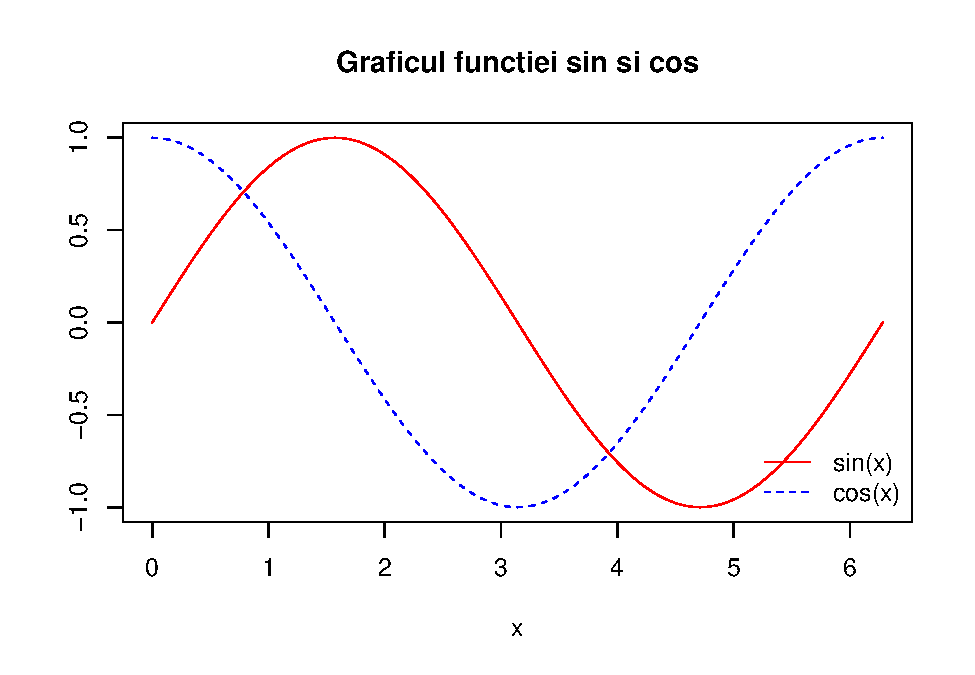
\includegraphics[width=0.8\linewidth]{Lab_1_files/figure-latex/unnamed-chunk-101-1} \end{center}

\subsection{Salvarea figurilor}\label{salvarea-figurilor}

Odată ce am creat un grafic putem să-l salvăm într-un fișier extern.
Pentru aceasta folosim funcțiile \texttt{pdf()}, \texttt{png()} sau
\texttt{jpeg()}. Aceste funcții vor salva figura ca fișier de tip .pdf,
.png sau .jpeg.

\begin{longtable}[]{@{}ll@{}}
\caption{Argumente pentru functiile pdf, jpeg si png}\tabularnewline
\toprule
\begin{minipage}[b]{0.14\columnwidth}\raggedright\strut
Argument\strut
\end{minipage} & \begin{minipage}[b]{0.71\columnwidth}\raggedright\strut
Rezultat\strut
\end{minipage}\tabularnewline
\midrule
\endfirsthead
\toprule
\begin{minipage}[b]{0.14\columnwidth}\raggedright\strut
Argument\strut
\end{minipage} & \begin{minipage}[b]{0.71\columnwidth}\raggedright\strut
Rezultat\strut
\end{minipage}\tabularnewline
\midrule
\endhead
\begin{minipage}[t]{0.14\columnwidth}\raggedright\strut
\texttt{file}\strut
\end{minipage} & \begin{minipage}[t]{0.71\columnwidth}\raggedright\strut
Directorul și numele fișierului sub formă de șir de caractere. De
exemplu, pentru a salva un grafic pe desktop scriem
\texttt{file\ =\ "/Users/.../Desktop/plot.pdf"} pentru un fișier
pdf.\strut
\end{minipage}\tabularnewline
\begin{minipage}[t]{0.14\columnwidth}\raggedright\strut
\texttt{width,\ height}\strut
\end{minipage} & \begin{minipage}[t]{0.71\columnwidth}\raggedright\strut
Dimensiunea graficului final în inchi.\strut
\end{minipage}\tabularnewline
\begin{minipage}[t]{0.14\columnwidth}\raggedright\strut
\texttt{dev.off()}\strut
\end{minipage} & \begin{minipage}[t]{0.71\columnwidth}\raggedright\strut
Acesta nu este un argument al funcțiilor \texttt{pdf()} și
\texttt{jpeg()}. Trebuie executat acest cod după ce trasarea graficului
a fost efectuată pentru a finaliza crearea imaginii.\strut
\end{minipage}\tabularnewline
\bottomrule
\end{longtable}

Pentru a salva o imagine avem de parcurs următorii pași:

\begin{enumerate}
\def\labelenumi{\arabic{enumi}.}
\tightlist
\item
  Execută funcțiile \texttt{pdf()} sau \texttt{jpeg()} cu argumentele
  \texttt{file,\ width,\ height}.
\item
  Execută codul care generează figura (e.g.
  \texttt{plot(x\ =\ 1:10,\ y\ =\ 1:10)})
\item
  Completează scrierea fișierului prin execuția comenzii
  \texttt{dev.off()}. Această comandă spune R-ului că am finalizat
  crearea fișierului.
\end{enumerate}

\begin{Shaded}
\begin{Highlighting}[]
\CommentTok{# Pasul 1}
\KeywordTok{pdf}\NormalTok{(}\DataTypeTok{file =} \StringTok{"/Users/.../Desktop/MyPlot.pdf"}\NormalTok{,   }\CommentTok{# directorul cu fisierul }
    \DataTypeTok{width =} \DecValTok{4}\NormalTok{, }\CommentTok{# latimea in inchi}
    \DataTypeTok{height =} \DecValTok{4}\NormalTok{) }\CommentTok{# inaltimea in inchi}

\CommentTok{# Pasul 2}
\KeywordTok{plot}\NormalTok{(}\DataTypeTok{x =} \DecValTok{1}\OperatorTok{:}\DecValTok{10}\NormalTok{, }
     \DataTypeTok{y =} \DecValTok{1}\OperatorTok{:}\DecValTok{10}\NormalTok{)}
\KeywordTok{abline}\NormalTok{(}\DataTypeTok{v =} \DecValTok{0}\NormalTok{) }
\KeywordTok{text}\NormalTok{(}\DataTypeTok{x =} \DecValTok{0}\NormalTok{, }\DataTypeTok{y =} \DecValTok{1}\NormalTok{, }\DataTypeTok{labels =} \StringTok{"Ceva text aleator"}\NormalTok{)}

\CommentTok{# Pasul 3}
\KeywordTok{dev.off}\NormalTok{()}
\end{Highlighting}
\end{Shaded}

\section{\texorpdfstring{Familia de funcții
\texttt{apply}}{Familia de funcții apply}}\label{familia-de-functii-apply}

Pe lângă buclele \texttt{for} și \texttt{while}, în R există și un set
de funcții care permit scrierea și rularea într-o manieră mai compactă a
codului dar și aplicarea de funcții unor grupuri de date.

\begin{itemize}
\item
  \texttt{lapply()}: Evaluează o funcție pentru fiecare element al unei
  liste
\item
  \texttt{sapply()}: La fel ca \texttt{lapply} numai că încearcă să
  simplifice rezultatul
\item
  \texttt{apply()}: Aplică o funcție după fiecare dimensiune a unui
  \texttt{array}
\item
  \texttt{tapply()}: Aplică o funcție pe submulțimi ale unui vector
\item
  \texttt{mapply()}: Varianta multivariată a funcției \texttt{lapply}
\item
  \texttt{split}: Împarte un vector în grupuri definite de o variabilă
  de tip factor.
\end{itemize}

\subsection{\texorpdfstring{\texttt{lapply()}}{lapply()}}\label{lapply}

Funcția \texttt{lapply()} efectuează următoarele operații:

\begin{enumerate}
\def\labelenumi{\arabic{enumi}.}
\tightlist
\item
  buclează după o listă, iterând după fiecare element din acea listă
\item
  aplică o \emph{funcție} fiecărui element al listei (o funcție pe care
  o specificăm)
\item
  întoarce ca rezultat tot o listă (prefixul \texttt{l} vine de la
  listă).
\end{enumerate}

Această funcție primește următoarele trei argument: (1) o listă
\texttt{X}; (2) o funcție \texttt{FUN}; (3) alte argumente via
\texttt{...}. Dacă \texttt{X} nu este o listă atunci aceasta va fi
transformată într-una folosind comanda \texttt{as.list()}.

Considerăm următorul exemplu în care vrem să aplicăm funcția
\texttt{mean()} tuturor elementelor unei liste

\begin{Shaded}
\begin{Highlighting}[]
\KeywordTok{set.seed}\NormalTok{(}\DecValTok{222}\NormalTok{)}
\NormalTok{x <-}\StringTok{ }\KeywordTok{list}\NormalTok{(}\DataTypeTok{a =} \DecValTok{1}\OperatorTok{:}\DecValTok{5}\NormalTok{, }\DataTypeTok{b =} \KeywordTok{rnorm}\NormalTok{(}\DecValTok{10}\NormalTok{), }\DataTypeTok{c =} \KeywordTok{rnorm}\NormalTok{(}\DecValTok{20}\NormalTok{, }\DecValTok{1}\NormalTok{), }\DataTypeTok{d =} \KeywordTok{rnorm}\NormalTok{(}\DecValTok{100}\NormalTok{, }\DecValTok{5}\NormalTok{))}
\KeywordTok{lapply}\NormalTok{(x, mean)}
\OperatorTok{$}\NormalTok{a}
\NormalTok{[}\DecValTok{1}\NormalTok{] }\DecValTok{3}

\OperatorTok{$}\NormalTok{b}
\NormalTok{[}\DecValTok{1}\NormalTok{] }\FloatTok{0.1996044}

\OperatorTok{$}\NormalTok{c}
\NormalTok{[}\DecValTok{1}\NormalTok{] }\FloatTok{0.7881026}

\OperatorTok{$}\NormalTok{d}
\NormalTok{[}\DecValTok{1}\NormalTok{] }\FloatTok{5.064188}
\end{Highlighting}
\end{Shaded}

Putem să folosim funcția \texttt{lapply()} pentru a evalua o funcție în
moduri repetate. Mai jos avem un exemplu în care folosim funcția
\texttt{runif()} (permite generarea observațiilor uniform repartizate)
de patru ori, de fiecare dată generăm un număr diferit de valori
aleatoare. Mai mult, argumentele \(min=0\) și \(max=3\) sunt atribuite,
prin intermediul argumentului \texttt{...}, funcției \texttt{runif}.

\begin{Shaded}
\begin{Highlighting}[]
\NormalTok{x <-}\StringTok{ }\DecValTok{1}\OperatorTok{:}\DecValTok{4}
\KeywordTok{lapply}\NormalTok{(x, runif, }\DataTypeTok{min =} \DecValTok{0}\NormalTok{, }\DataTypeTok{max =} \DecValTok{3}\NormalTok{)}
\NormalTok{[[}\DecValTok{1}\NormalTok{]]}
\NormalTok{[}\DecValTok{1}\NormalTok{] }\FloatTok{0.03443616}

\NormalTok{[[}\DecValTok{2}\NormalTok{]]}
\NormalTok{[}\DecValTok{1}\NormalTok{] }\FloatTok{1.267361} \FloatTok{1.365441}

\NormalTok{[[}\DecValTok{3}\NormalTok{]]}
\NormalTok{[}\DecValTok{1}\NormalTok{] }\FloatTok{1.8084700} \FloatTok{2.1902665} \FloatTok{0.4139585}

\NormalTok{[[}\DecValTok{4}\NormalTok{]]}
\NormalTok{[}\DecValTok{1}\NormalTok{] }\FloatTok{1.5924650} \FloatTok{0.7355067} \FloatTok{2.1483841} \FloatTok{1.6082945}
\end{Highlighting}
\end{Shaded}

\subsection{\texorpdfstring{\texttt{sapply()}}{sapply()}}\label{sapply}

Funcția \texttt{sapply()} are un comportament similar cu
\texttt{lapply()} prin faptul că funcția \texttt{sapply()} apelează
intern \texttt{lapply()} pentru valorile de input, după care evaluează:

\begin{itemize}
\item
  dacă rezultatul este o listă în care fiecare element este de lungime
  1, atunci întoarce un vector
\item
  dacă rezultatul este o listă în care fiecare element este un vector de
  aceeași lungime (\textgreater{}1), se întoarce o matrice
\item
  în caz contrar se întoarce o listă.
\end{itemize}

Considerăm exemplul de mai sus

\begin{Shaded}
\begin{Highlighting}[]
\KeywordTok{set.seed}\NormalTok{(}\DecValTok{222}\NormalTok{)}
\NormalTok{x <-}\StringTok{ }\KeywordTok{list}\NormalTok{(}\DataTypeTok{a =} \DecValTok{1}\OperatorTok{:}\DecValTok{4}\NormalTok{, }\DataTypeTok{b =} \KeywordTok{rnorm}\NormalTok{(}\DecValTok{10}\NormalTok{), }\DataTypeTok{c =} \KeywordTok{rnorm}\NormalTok{(}\DecValTok{20}\NormalTok{, }\DecValTok{1}\NormalTok{), }\DataTypeTok{d =} \KeywordTok{rnorm}\NormalTok{(}\DecValTok{100}\NormalTok{, }\DecValTok{5}\NormalTok{))}
\KeywordTok{sapply}\NormalTok{(x, mean)}
\NormalTok{        a         b         c         d }
\FloatTok{2.5000000} \FloatTok{0.1996044} \FloatTok{0.7881026} \FloatTok{5.0641876} 
\end{Highlighting}
\end{Shaded}

\subsection{\texorpdfstring{\texttt{split()}}{split()}}\label{split}

Funcția \texttt{split()} primește ca argument un vector sau o listă (sau
un data.frame) și împarte datele în grupuri determinate de o variabilă
de tip factor (sau o listă de factor).

Argumentele aceste funcții sunt

\begin{Shaded}
\begin{Highlighting}[]
\KeywordTok{str}\NormalTok{(split)}
\ControlFlowTok{function}\NormalTok{ (x, f, }\DataTypeTok{drop =} \OtherTok{FALSE}\NormalTok{, ...)  }
\end{Highlighting}
\end{Shaded}

unde

\begin{itemize}
\tightlist
\item
  \texttt{x} este un vector, o listă sau un data.frame
\item
  \texttt{f} este un factor sau o listă de factori
\end{itemize}

Considerăm următorul exemplu în care generăm un vector de date și îl
împărțim după o variabilă de tip factor creată cu ajutorul funcției
\texttt{gl()} (\emph{generate levels}).

\begin{Shaded}
\begin{Highlighting}[]
\NormalTok{x <-}\StringTok{ }\KeywordTok{c}\NormalTok{(}\KeywordTok{rnorm}\NormalTok{(}\DecValTok{10}\NormalTok{), }\KeywordTok{runif}\NormalTok{(}\DecValTok{10}\NormalTok{), }\KeywordTok{rnorm}\NormalTok{(}\DecValTok{10}\NormalTok{, }\DecValTok{1}\NormalTok{))}
\NormalTok{f <-}\StringTok{ }\KeywordTok{gl}\NormalTok{(}\DecValTok{3}\NormalTok{, }\DecValTok{10}\NormalTok{)}
\KeywordTok{split}\NormalTok{(x, f)}
\OperatorTok{$}\StringTok{`}\DataTypeTok{1}\StringTok{`}
\NormalTok{ [}\DecValTok{1}\NormalTok{] }\OperatorTok{-}\FloatTok{2.27414224} \OperatorTok{-}\FloatTok{0.11266780}  \FloatTok{0.61308167}  \FloatTok{0.07733545}  \FloatTok{0.57137727}
\NormalTok{ [}\DecValTok{6}\NormalTok{]  }\FloatTok{0.11672493} \OperatorTok{-}\FloatTok{0.95685256} \OperatorTok{-}\FloatTok{1.90008460} \OperatorTok{-}\FloatTok{1.48972089}  \FloatTok{0.55925676}

\OperatorTok{$}\StringTok{`}\DataTypeTok{2}\StringTok{`}
\NormalTok{ [}\DecValTok{1}\NormalTok{] }\FloatTok{0.91159086} \FloatTok{0.03291829} \FloatTok{0.78368939} \FloatTok{0.11852882} \FloatTok{0.64443831} \FloatTok{0.78790988}
\NormalTok{ [}\DecValTok{7}\NormalTok{] }\FloatTok{0.82451477} \FloatTok{0.05642366} \FloatTok{0.65075027} \FloatTok{0.95426854}

\OperatorTok{$}\StringTok{`}\DataTypeTok{3}\StringTok{`}
\NormalTok{ [}\DecValTok{1}\NormalTok{]  }\FloatTok{2.6666242}  \FloatTok{2.6634334}  \FloatTok{1.8106280} \OperatorTok{-}\FloatTok{0.7837308}  \FloatTok{1.6575684}  \FloatTok{0.1546575}
\NormalTok{ [}\DecValTok{7}\NormalTok{]  }\FloatTok{0.4930056} \OperatorTok{-}\FloatTok{0.9031544}  \FloatTok{2.4042311}  \FloatTok{1.4106863}
\end{Highlighting}
\end{Shaded}

Putem folosi funcția \texttt{split} și în conjuncție cu funcția
\texttt{lapply} (atunci când vrem să aplicăm o funcție \texttt{FUN} pe
grupuri de date).

\begin{Shaded}
\begin{Highlighting}[]
\KeywordTok{lapply}\NormalTok{(}\KeywordTok{split}\NormalTok{(x, f), mean)}
\OperatorTok{$}\StringTok{`}\DataTypeTok{1}\StringTok{`}
\NormalTok{[}\DecValTok{1}\NormalTok{] }\OperatorTok{-}\FloatTok{0.4795692}

\OperatorTok{$}\StringTok{`}\DataTypeTok{2}\StringTok{`}
\NormalTok{[}\DecValTok{1}\NormalTok{] }\FloatTok{0.5765033}

\OperatorTok{$}\StringTok{`}\DataTypeTok{3}\StringTok{`}
\NormalTok{[}\DecValTok{1}\NormalTok{] }\FloatTok{1.157395}
\end{Highlighting}
\end{Shaded}

\subsection{\texorpdfstring{\texttt{tapply()}}{tapply()}}\label{tapply}

Funcția \texttt{tapply()} este folosită pentru aplicarea unei funcții
\texttt{FUN} pe submulțimile unui vector și poate fi văzută ca o
combinație între \texttt{split()} și \texttt{sapply()}, dar doar pentru
vectori.

\begin{Shaded}
\begin{Highlighting}[]
\KeywordTok{str}\NormalTok{(tapply)}
\ControlFlowTok{function}\NormalTok{ (X, INDEX, }\DataTypeTok{FUN =} \OtherTok{NULL}\NormalTok{, ..., }\DataTypeTok{default =} \OtherTok{NA}\NormalTok{, }\DataTypeTok{simplify =} \OtherTok{TRUE}\NormalTok{)  }
\end{Highlighting}
\end{Shaded}

Argumentele acestei funcții sunt date de următorul tabel:

\begin{longtable}[]{@{}ll@{}}
\caption{Argumentele functiei tapply}\tabularnewline
\toprule
Argument & Descriere\tabularnewline
\midrule
\endfirsthead
\toprule
Argument & Descriere\tabularnewline
\midrule
\endhead
\texttt{X} & un vector\tabularnewline
\texttt{INDEX} & este o variabilă de tip factor sau o listă de
factori\tabularnewline
\texttt{FUN} & o funcție ce urmează să fie aplicată\tabularnewline
\texttt{...} & argumente ce vor fi atribuite funcției
\texttt{FUN}\tabularnewline
\texttt{simplify} & dacă vrem să simplificăm rezultatul\tabularnewline
\bottomrule
\end{longtable}

Următorul exemplu calculează media după fiecare grupă determinată de o
variabilă de tip factor a unui vector numeric.

\begin{Shaded}
\begin{Highlighting}[]
\NormalTok{x <-}\StringTok{ }\KeywordTok{c}\NormalTok{(}\KeywordTok{rnorm}\NormalTok{(}\DecValTok{10}\NormalTok{), }\KeywordTok{runif}\NormalTok{(}\DecValTok{10}\NormalTok{), }\KeywordTok{rnorm}\NormalTok{(}\DecValTok{10}\NormalTok{, }\DecValTok{1}\NormalTok{))}
\NormalTok{f <-}\StringTok{ }\KeywordTok{gl}\NormalTok{(}\DecValTok{3}\NormalTok{, }\DecValTok{10}\NormalTok{)   }
\NormalTok{f}
\NormalTok{ [}\DecValTok{1}\NormalTok{] }\DecValTok{1} \DecValTok{1} \DecValTok{1} \DecValTok{1} \DecValTok{1} \DecValTok{1} \DecValTok{1} \DecValTok{1} \DecValTok{1} \DecValTok{1} \DecValTok{2} \DecValTok{2} \DecValTok{2} \DecValTok{2} \DecValTok{2} \DecValTok{2} \DecValTok{2} \DecValTok{2} \DecValTok{2} \DecValTok{2} \DecValTok{3} \DecValTok{3} \DecValTok{3} \DecValTok{3} \DecValTok{3} \DecValTok{3} \DecValTok{3} \DecValTok{3} \DecValTok{3} \DecValTok{3}
\NormalTok{Levels}\OperatorTok{:}\StringTok{ }\DecValTok{1} \DecValTok{2} \DecValTok{3}
\KeywordTok{tapply}\NormalTok{(x, f, mean)}
            \DecValTok{1}             \DecValTok{2}             \DecValTok{3} 
\OperatorTok{-}\FloatTok{0.0007774025}  \FloatTok{0.3736457792}  \FloatTok{0.5789436983} 
\end{Highlighting}
\end{Shaded}

Putem să aplicăm și funcții care întorc mai mult de un rezultat. În
această situație rezultatul nu poate fi simplificat:

\begin{Shaded}
\begin{Highlighting}[]
\KeywordTok{tapply}\NormalTok{(x, f, range)}
\OperatorTok{$}\StringTok{`}\DataTypeTok{1}\StringTok{`}
\NormalTok{[}\DecValTok{1}\NormalTok{] }\OperatorTok{-}\FloatTok{2.1904113}  \FloatTok{0.9249901}

\OperatorTok{$}\StringTok{`}\DataTypeTok{2}\StringTok{`}
\NormalTok{[}\DecValTok{1}\NormalTok{] }\FloatTok{0.004445296} \FloatTok{0.998309704}

\OperatorTok{$}\StringTok{`}\DataTypeTok{3}\StringTok{`}
\NormalTok{[}\DecValTok{1}\NormalTok{] }\OperatorTok{-}\FloatTok{0.3379675}  \FloatTok{1.9327099}
\end{Highlighting}
\end{Shaded}

\subsection{\texorpdfstring{\texttt{apply()}}{apply()}}\label{apply}

Funcția \texttt{apply()} este folosită cu precădere pentru a aplica o
funcție liniilor și coloanelor unei matrice (care este un \texttt{array}
bidimensional). Cu toate acestea poate fi folosită pe tablouri
multidimensionale (\texttt{array}) în general. Folosirea funcției
\texttt{apply()} nu este mai rapidă decât scrierea unei bucle
\texttt{for}, dar este mai compactă.

\begin{Shaded}
\begin{Highlighting}[]
\KeywordTok{str}\NormalTok{(apply)}
\ControlFlowTok{function}\NormalTok{ (X, MARGIN, FUN, ...)  }
\end{Highlighting}
\end{Shaded}

Argumentele funcției \texttt{apply()} sunt

\begin{itemize}
\tightlist
\item
  \texttt{X} un tablou multidimensional
\item
  \texttt{MARGIN} este un vector numeric care indică dimensiunea sau
  dimensiunile după care se va aplica funcția
\item
  \texttt{FUN} este o funcție ce urmează să fie aplicată
\item
  \texttt{...} alte argumente penru funcția\texttt{FUN}
\end{itemize}

Considerăm următorul exemplu în care calculăm media pe coloane într-o
matrice

\begin{Shaded}
\begin{Highlighting}[]
\NormalTok{x <-}\StringTok{ }\KeywordTok{matrix}\NormalTok{(}\KeywordTok{rnorm}\NormalTok{(}\DecValTok{200}\NormalTok{), }\DecValTok{20}\NormalTok{, }\DecValTok{10}\NormalTok{)}
\KeywordTok{apply}\NormalTok{(x, }\DecValTok{2}\NormalTok{, mean)  ## media fiecarei coloane}
\NormalTok{ [}\DecValTok{1}\NormalTok{]  }\FloatTok{3.745002e-02}  \FloatTok{1.857656e-01} \OperatorTok{-}\FloatTok{2.413659e-01} \OperatorTok{-}\FloatTok{2.093141e-01} \OperatorTok{-}\FloatTok{2.562272e-01}
\NormalTok{ [}\DecValTok{6}\NormalTok{]  }\FloatTok{8.986712e-05}  \FloatTok{7.444137e-02} \OperatorTok{-}\FloatTok{7.460941e-03}  \FloatTok{6.275282e-02}  \FloatTok{9.801550e-02}
\end{Highlighting}
\end{Shaded}

precum și media după fiecare linie

\begin{Shaded}
\begin{Highlighting}[]
\KeywordTok{apply}\NormalTok{(x, }\DecValTok{1}\NormalTok{, sum)   ## media fiecarei linii}
\NormalTok{ [}\DecValTok{1}\NormalTok{]  }\FloatTok{2.76179139}  \FloatTok{2.53107681}  \FloatTok{0.87923177}  \FloatTok{1.80480589}  \FloatTok{0.98225832}
\NormalTok{ [}\DecValTok{6}\NormalTok{] }\OperatorTok{-}\FloatTok{3.06148753} \OperatorTok{-}\FloatTok{1.40358820} \OperatorTok{-}\FloatTok{0.65969812} \OperatorTok{-}\FloatTok{1.63717046} \OperatorTok{-}\FloatTok{0.29330726}
\NormalTok{[}\DecValTok{11}\NormalTok{] }\OperatorTok{-}\FloatTok{2.41486442} \OperatorTok{-}\FloatTok{3.15698523}  \FloatTok{2.27126822} \OperatorTok{-}\FloatTok{3.88290287} \OperatorTok{-}\FloatTok{3.15595194}
\NormalTok{[}\DecValTok{16}\NormalTok{]  }\FloatTok{5.41211963}  \FloatTok{2.32985530} \OperatorTok{-}\FloatTok{3.05330574} \OperatorTok{-}\FloatTok{0.02110926} \OperatorTok{-}\FloatTok{1.34909559}
\end{Highlighting}
\end{Shaded}

\section{Repartiții și elemente aleatoare în
R}\label{repartitii-si-elemente-aleatoare-in-r}

R pune la disploziție majoritatea repartițiilor uzuale. Tabelul de mai
jos prezintă numele și parametrii acestora:

\begin{longtable}[]{@{}llll@{}}
\caption{Numele si parametrii repartitiilor uzuale in R}\tabularnewline
\toprule
Repartiția & Nume & Parametrii & Valori prestabilite\tabularnewline
\midrule
\endfirsthead
\toprule
Repartiția & Nume & Parametrii & Valori prestabilite\tabularnewline
\midrule
\endhead
Beta & \texttt{beta} & \texttt{shape1}, \texttt{shape2} &\tabularnewline
Binomial & \texttt{binom} & \texttt{size}, \texttt{prob}
&\tabularnewline
Cauchy & \texttt{cauchy} & \texttt{location}, \texttt{scale} &
\texttt{location\ =\ 0}, \texttt{scale\ =\ 1}\tabularnewline
Chi-Squared & \texttt{chisq} & \texttt{df} &\tabularnewline
Exponential & \texttt{exp} & \texttt{rate} (=1/mean) &
\texttt{rate\ =\ 1}\tabularnewline
Fisher & \texttt{f} & \texttt{df1}, \texttt{df2} &\tabularnewline
Gamma & \texttt{gamma} & \texttt{shape}, \texttt{rate} (=1/scale) &
\texttt{rate\ =\ 1}\tabularnewline
Hypergeometric & \texttt{hyper} & \texttt{m}, \texttt{n}, \texttt{k}
&\tabularnewline
Log-Normal & \texttt{lnorm} & \texttt{mean}, \texttt{sd} &
\texttt{mean\ =\ 0}, \texttt{sd\ =\ 1}\tabularnewline
Logistic & \texttt{logis} & \texttt{location}, \texttt{scale} &
\texttt{location\ =\ 0}, \texttt{scale\ =\ 1}\tabularnewline
Normal & \texttt{norm} & \texttt{mean}, \texttt{sd} &
\texttt{mean\ =\ 0}, \texttt{sd\ =\ 1}\tabularnewline
Poisson & \texttt{pois} & \texttt{lambda} &\tabularnewline
Student & \texttt{t} & \texttt{df} &\tabularnewline
Uniform & \texttt{unif} & \texttt{min}, \texttt{max} &
\texttt{min\ =\ 0}, \texttt{max\ =\ 1}\tabularnewline
Weibull & \texttt{weibull} & \texttt{shape} &\tabularnewline
\bottomrule
\end{longtable}

Pentru fiecare repartiție, există patru comenzi în R prefixate cu
literele \texttt{d}, \texttt{p}, \texttt{q} și \texttt{r} și urmate de
numele repartiției (coloana a 2-a). De exemplu \texttt{dnorm},
\texttt{pnorm}, \texttt{qnorm} și \texttt{rnorm} sunt comenzile
corespunzătoare repartiției normale pe când \texttt{dunif},
\texttt{punif}, \texttt{qunif} și \texttt{runif} sunt cele
corespunzătoare repartiției uniforme.

\begin{itemize}
\item
  \texttt{dname}: calculează densitatea atunci când vorbim de o
  variabilă continue sau funcția de masă atunci când avem o repartiție
  discretă (\(\mathbb{P}(X=k)\))
\item
  \texttt{pname}: calculează funcția de repartiție, i.e.
  \(F(x)=\mathbb{P}(X\leq x)\)
\item
  \texttt{qname}: reprezintă funcția cuantilă, cu alte cuvinte valoarea
  pentru care funcția de repartiție are o anumită probabilitate; în
  cazul continuu, dacă \texttt{pname(x)\ =\ p} atunci
  \texttt{qname(p)\ =\ x} iar în cazul discret întoarce cel mai mic
  întreg \(u\) pentru care \(\mathbb{P}(X\leq u)\geq p\).
\item
  \texttt{rname}: generează observații independente din repartiția dată
\end{itemize}

O parte din cele mai cunoscute repartiții continue (pentru mai multe
informații, se poate consulta monografia (Johnson, Kotz, and
Balakrishnan 1994)) sunt prezentate mai jos:

\subsection{Repartiția Uniformă}\label{repartitia-uniforma}

O variabilă aleatoare \(X\) repartizată \emph{uniform} pe intervalul
\([a,b]\), notată \(X\sim \mathcal{U}[a,b]\), are densitatea dată de

\[
  f_X(x) = \left\{\begin{array}{ll}
    \frac{1}{b-a}, & x\in[a,b]\\
    0, & \text{altfel}
  \end{array}\right.
\]

\begin{center}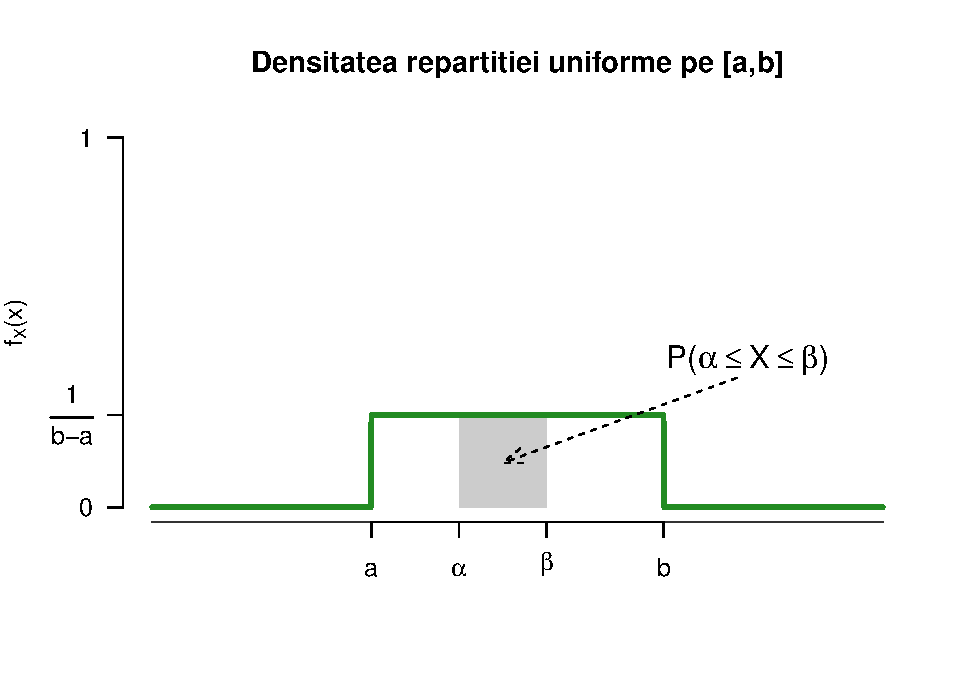
\includegraphics[width=0.7\linewidth]{Lab_1_files/figure-latex/unnamed-chunk-115-1} \end{center}

Funcția de repartiție a repartiției uniforme este

\[
  F_X(x) =\int_{-\infty}^{x}f_X(t)\,dt = \left\{\begin{array}{ll}
    0, & x\leq a\\
    \frac{x-a}{b-a}, & x\in(a,b)\\
    1, & x\geq b
  \end{array}\right.
\]

\begin{center}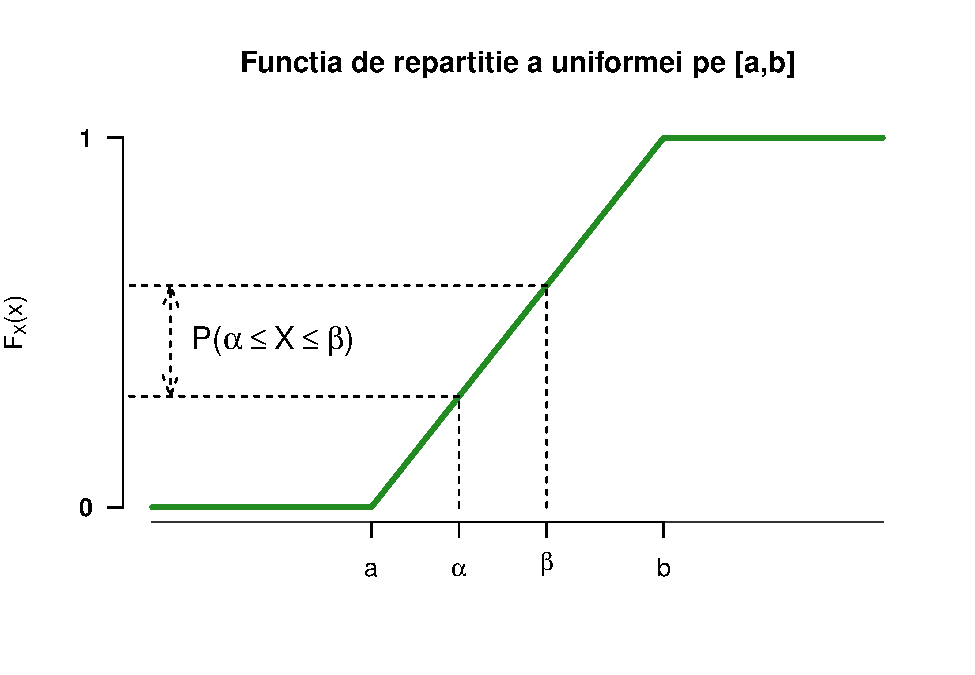
\includegraphics[width=0.7\linewidth]{Lab_1_files/figure-latex/unnamed-chunk-116-1} \end{center}

Media și varianța variabilei aleatoare \(X\) repartizate uniform pe
\([a,b]\) sunt egale cu

\[
  \mathbb{E}[X] = \frac{a+b}{2},\qquad Var(X) = \frac{(a-b)^2}{12}. 
\]

Variabilele aleatoare repartizate uniform joacă un rol important în
teoria simulării variabilelor aleatoare datorită următorului rezultat
datorat lui Paul Levy și numit \emph{teorema de universalitate a
repartiției uniforme}:

\begin{rmdinsight}
Fie \(X\) o variabilă aleatoare reală cu funcția de repartiție \(F\),
\(U\) o variabilă aleatoare repartizată uniform pe \([0,1]\) și fie
funcția \emph{cuantilă} (inversa generalizată) asociată lui \(F\),
\(F^{-1}:(0,1)\to\mathbb{R}\) definită prin

\[
  F^{-1}(u) = \inf\{x\in\mathbb{R}\,|\,F(x)\geq u\}, \quad \forall u\in(0,1).
\] Atunci \(X\) și \(F^{-1}(U)\) sunt repartizate la fel.
\end{rmdinsight}

În R putem să

\begin{itemize}
\tightlist
\item
  generăm observații independente din repartiția \(\mathcal{U}([a, b])\)
  (e.g. \(a = 3\) și \(b = 5\))
\end{itemize}

\begin{Shaded}
\begin{Highlighting}[]
\KeywordTok{runif}\NormalTok{(}\DecValTok{10}\NormalTok{, }\DecValTok{3}\NormalTok{, }\DecValTok{5}\NormalTok{)}
\NormalTok{ [}\DecValTok{1}\NormalTok{] }\FloatTok{4.333149} \FloatTok{3.781585} \FloatTok{4.599373} \FloatTok{4.075318} \FloatTok{4.949425} \FloatTok{4.817059} \FloatTok{4.894950}
\NormalTok{ [}\DecValTok{8}\NormalTok{] }\FloatTok{3.030199} \FloatTok{4.964791} \FloatTok{4.941631}
\end{Highlighting}
\end{Shaded}

\begin{itemize}
\tightlist
\item
  calculăm densitatea unei variabile aleatoare repartizate uniform pe
  \([a, b]\) în diferite puncte
\end{itemize}

\begin{Shaded}
\begin{Highlighting}[]
\KeywordTok{dunif}\NormalTok{(}\KeywordTok{c}\NormalTok{(}\FloatTok{3.1}\NormalTok{, }\FloatTok{3.7}\NormalTok{, }\FloatTok{3.95}\NormalTok{, }\FloatTok{4.86}\NormalTok{), }\DecValTok{3}\NormalTok{, }\DecValTok{5}\NormalTok{)}
\NormalTok{[}\DecValTok{1}\NormalTok{] }\FloatTok{0.5} \FloatTok{0.5} \FloatTok{0.5} \FloatTok{0.5}
\end{Highlighting}
\end{Shaded}

\begin{itemize}
\tightlist
\item
  calculăm funcția de repartiție a unei variabile repartizate uniform pe
  \([a,b]\) pentru diferite valori
\end{itemize}

\begin{Shaded}
\begin{Highlighting}[]
\KeywordTok{punif}\NormalTok{(}\KeywordTok{c}\NormalTok{(}\FloatTok{3.1}\NormalTok{, }\FloatTok{3.7}\NormalTok{, }\FloatTok{3.95}\NormalTok{, }\FloatTok{4.86}\NormalTok{), }\DecValTok{3}\NormalTok{, }\DecValTok{5}\NormalTok{)}
\NormalTok{[}\DecValTok{1}\NormalTok{] }\FloatTok{0.050} \FloatTok{0.350} \FloatTok{0.475} \FloatTok{0.930}
\end{Highlighting}
\end{Shaded}

\begin{rmdexercise}
Fie \(X\) o variabilă aleatoare repartizată uniform pe \([2,7]\).
Determinați:

\begin{enumerate}
\def\labelenumi{\alph{enumi})}
\tightlist
\item
  \(\mathbb{P}(X\in\{1,2,3,4,5,6,7\})\)
\item
  \(\mathbb{P}(X<3)\) și \(\mathbb{P}(X\leq 3)\)
\item
  \(\mathbb{P}(X\leq 3 \cup X>4)\)
\item
  Generați \(250\) de observații din repartiția dată, trasați histograma
  acestora și suprapuneți densitatea repartiției date (vezi figura de
  mai jos).
\end{enumerate}
\end{rmdexercise}

\begin{center}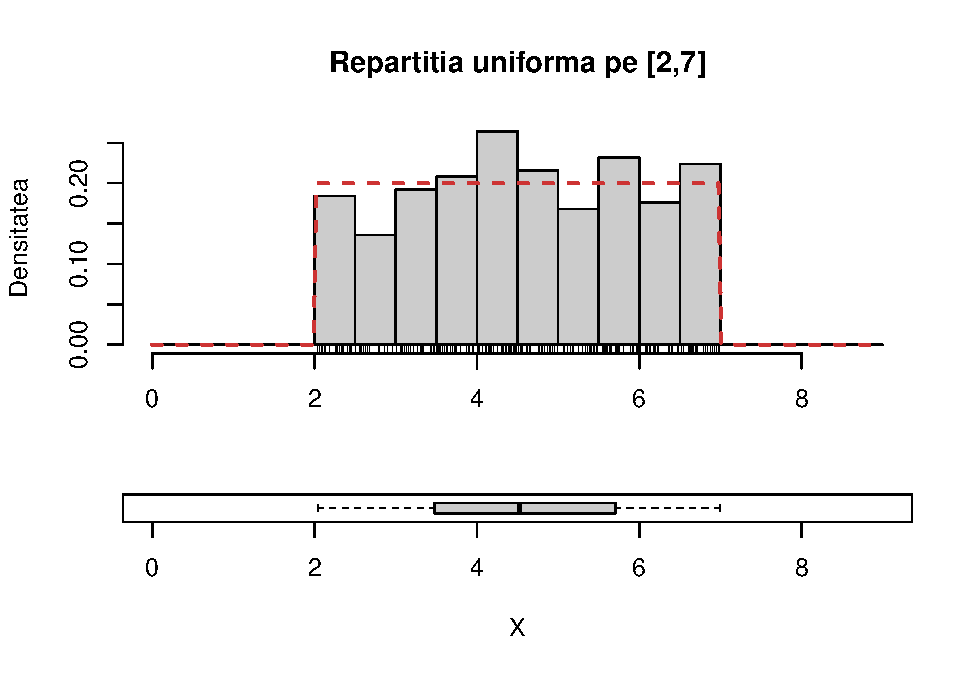
\includegraphics[width=0.7\linewidth]{Lab_1_files/figure-latex/unnamed-chunk-122-1} \end{center}

\begin{rmdexercise}
Dacă \(X\) o variabilă aleatoare repartizată uniform pe \([a,b]\) și
\([c,d]\subset [a,b]\) este un subinterval, atunci repartiția
condiționată a lui \(X\) la \(X\in [c,d]\) este \(\mathcal{U}[c,d]\).
\end{rmdexercise}

\subsection{Repartiția Normală}\label{repartitia-normala}

Spunem că o variabilă aleatoare \(X\) este repartizată \emph{normal} sau
\emph{Gaussian} de medie \(\mu\) și varianță \(\sigma^2\), și se notează
cu \(X\sim\mathcal{N}(\mu, \sigma^2)\), dacă densitatea ei are forma

\[
  f_X(x) \left(\overset{not}{=} \varphi(x)\right) = \frac{1}{\sqrt{2\pi}\sigma}e^{-\frac{(x-\mu)^2}{2\sigma^2}}, \quad x\in\mathbb{R}.
\]

\begin{center}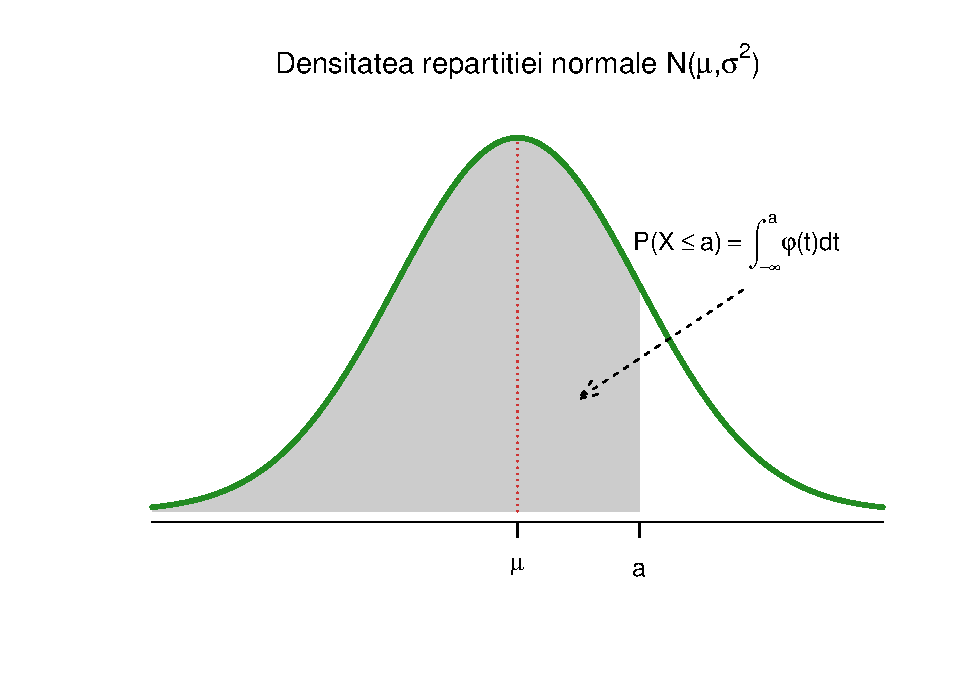
\includegraphics[width=0.7\linewidth]{Lab_1_files/figure-latex/unnamed-chunk-124-1} \end{center}

Funcția de repartiție a unei variabile
\(X\sim\mathcal{N}(\mu, \sigma^2)\) este dată de

\[
  F_X(x) \left(\overset{not}{=} \Phi(x)\right) = \int_{-\infty}^{x}\varphi(t)\,dt = \frac{1}{\sqrt{2\pi}\sigma}\int_{-\infty}^{x}e^{-\frac{(t-\mu)^2}{2\sigma^2}}\,dt.
\]

Pentru funcția de repartiție nu avem o formulă explicită de calcul, ea
poate fi aproximată cu ajutorul descompunerii în serie. În cazul
variabilelor \emph{normale standard} (\(X\sim\mathcal{N}(0,1)\)) avem
proprietățile (pentru mai multe astfel de inegalități se poate consulta
cartea (Lin and Bai 2010, capitolul 2))

\begin{enumerate}
\def\labelenumi{\alph{enumi})}
\tightlist
\item
  \(\Phi(x) = 1-\Phi(-x)\) pentru toate valorile \(x\in\mathbb{R}\)
\item
  \(1-\Phi(a)\leq\frac{1}{2}e^{-\frac{a^2}{2}}\) pentru
  \(a>0\)\footnote{Pentru mai multe astfel de inegalități se poate
    consulta cartea (capitolul 2): Lin, Z. și Bai, Z. \emph{Probability
    Inequalities}, Springer, 2010.}
\end{enumerate}

\begin{center}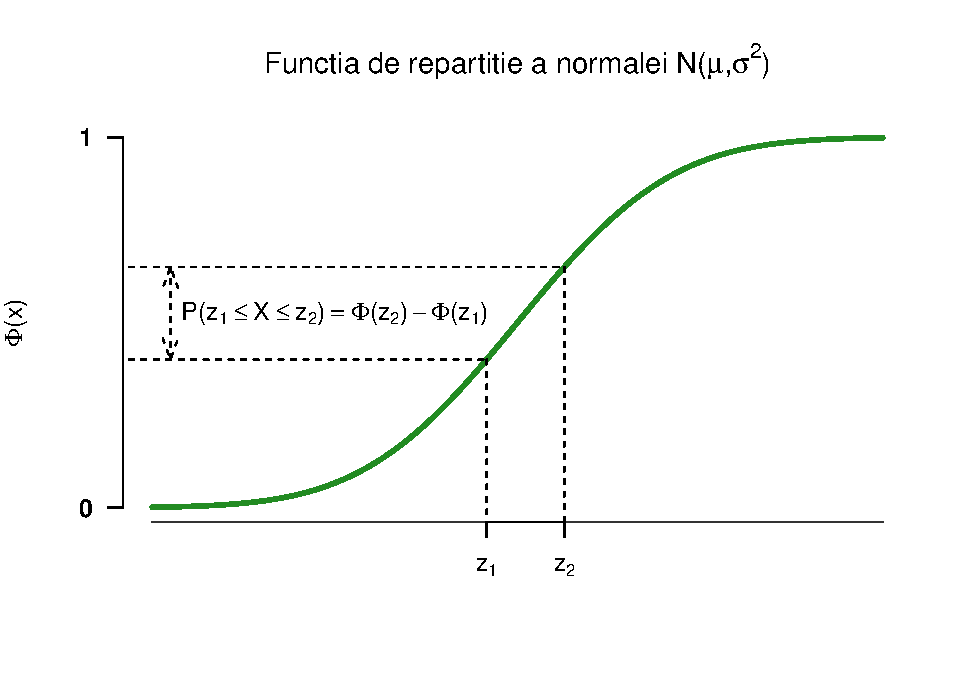
\includegraphics[width=0.7\linewidth]{Lab_1_files/figure-latex/unnamed-chunk-125-1} \end{center}

Media și varianța variabilei aleatoare \(X\) repartizate normal de
parametrii \(\mathcal{N}(\mu, \sigma^2)\) sunt egale cu

\[
  \mathbb{E}[X] = \mu,\quad Var(X) = \sigma^2. 
\] Mai mult, momentele de ordin se pot calcula cu ușurință și avem că

\[
  \mathbb{E}[X^k] = \left\{\begin{array}{ll}
      \sigma^k (k-1)!!, & \text{$k$ este par} \\
      0, & \text{$k$ este impar}.
  \end{array}\right.
\]

Pentru o variabilă aleatoare repartizată normal, avem următoarea regulă
numită și regula \(68-95-99.7\%\):

\begin{rmdinsight}
Fie \(X\) o variabilă aleatoare repartizată
\(\mathcal{N}(\mu, \sigma^2)\). Atunci

\begin{align*}
  \mathbb{P}(|X-\mu|<\sigma) &\approx 0.68\\
  \mathbb{P}(|X-\mu|<2\sigma) &\approx 0.95\\
  \mathbb{P}(|X-\mu|<3\sigma) &\approx 0.997
\end{align*}
\end{rmdinsight}

În R putem să

\begin{itemize}
\tightlist
\item
  generăm observații independente din repartiția
  \(\mathcal{N}(\mu, \sigma^2)\) (e.g. \(\mu = 0\) și \(\sigma^2 = 2\) -
  în R funcțiile \texttt{rnorm}, \texttt{dnorm}, \texttt{pnorm} și
  \texttt{qnorm} primesc ca parametrii media și abaterea standard,
  \(\sigma\) \textbf{nu} varianța \(\sigma^2\))
\end{itemize}

\begin{Shaded}
\begin{Highlighting}[]
\KeywordTok{rnorm}\NormalTok{(}\DecValTok{10}\NormalTok{, }\DataTypeTok{mean =} \DecValTok{0}\NormalTok{, }\DataTypeTok{sd =} \KeywordTok{sqrt}\NormalTok{(}\DecValTok{2}\NormalTok{))}
\NormalTok{ [}\DecValTok{1}\NormalTok{]  }\FloatTok{3.24538640}  \FloatTok{2.72962533}  \FloatTok{2.63876613} \OperatorTok{-}\FloatTok{3.68120130} \OperatorTok{-}\FloatTok{0.80807440}
\NormalTok{ [}\DecValTok{6}\NormalTok{]  }\FloatTok{0.06325232} \OperatorTok{-}\FloatTok{1.67041553} \OperatorTok{-}\FloatTok{2.71001645} \OperatorTok{-}\FloatTok{2.08833178} \OperatorTok{-}\FloatTok{0.74799126}
\end{Highlighting}
\end{Shaded}

\begin{itemize}
\tightlist
\item
  calculăm densitatea unei variabile aleatoare repartizate normal
  \(\mathcal{N}(\mu, \sigma^2)\) în diferite puncte
\end{itemize}

\begin{Shaded}
\begin{Highlighting}[]
\KeywordTok{dnorm}\NormalTok{(}\KeywordTok{seq}\NormalTok{(}\OperatorTok{-}\DecValTok{2}\NormalTok{, }\DecValTok{2}\NormalTok{, }\DataTypeTok{length.out =} \DecValTok{15}\NormalTok{), }\DataTypeTok{mean =} \DecValTok{3}\NormalTok{, }\DataTypeTok{sd =} \DecValTok{5}\NormalTok{)}
\NormalTok{ [}\DecValTok{1}\NormalTok{] }\FloatTok{0.04839414} \FloatTok{0.05115647} \FloatTok{0.05390019} \FloatTok{0.05660592} \FloatTok{0.05925368} \FloatTok{0.06182308}
\NormalTok{ [}\DecValTok{7}\NormalTok{] }\FloatTok{0.06429362} \FloatTok{0.06664492} \FloatTok{0.06885700} \FloatTok{0.07091058} \FloatTok{0.07278734} \FloatTok{0.07447021}
\NormalTok{[}\DecValTok{13}\NormalTok{] }\FloatTok{0.07594361} \FloatTok{0.07719368} \FloatTok{0.07820854}
\end{Highlighting}
\end{Shaded}

\begin{itemize}
\tightlist
\item
  calculăm funcția de repartiție a unei variabile repartizate normal
  \(\mathcal{N}(\mu, \sigma^2)\) pentru diferite valori
\end{itemize}

\begin{Shaded}
\begin{Highlighting}[]
\KeywordTok{pnorm}\NormalTok{(}\KeywordTok{seq}\NormalTok{(}\OperatorTok{-}\DecValTok{1}\NormalTok{, }\DecValTok{1}\NormalTok{, }\DataTypeTok{length.out =} \DecValTok{15}\NormalTok{), }\DataTypeTok{mean =} \DecValTok{3}\NormalTok{, }\DataTypeTok{sd =} \DecValTok{1}\NormalTok{)}
\NormalTok{ [}\DecValTok{1}\NormalTok{] }\FloatTok{3.167124e-05} \FloatTok{5.736006e-05} \FloatTok{1.018892e-04} \FloatTok{1.775197e-04} \FloatTok{3.033834e-04}
\NormalTok{ [}\DecValTok{6}\NormalTok{] }\FloatTok{5.086207e-04} \FloatTok{8.365374e-04} \FloatTok{1.349898e-03} \FloatTok{2.137367e-03} \FloatTok{3.320943e-03}
\NormalTok{[}\DecValTok{11}\NormalTok{] }\FloatTok{5.063995e-03} \FloatTok{7.579219e-03} \FloatTok{1.113549e-02} \FloatTok{1.606229e-02} \FloatTok{2.275013e-02}
\end{Highlighting}
\end{Shaded}

\begin{itemize}
\tightlist
\item
  calculăm cuantilele de ordin \(\alpha\in(0,1)\) (i.e.~valoarea
  \(z_{\alpha}\) pentru care \(\Phi(z_{\alpha}) = \alpha\) sau altfel
  spus \(z_{\alpha} = \Phi^{-1}(\alpha)\))
\end{itemize}

\begin{Shaded}
\begin{Highlighting}[]
\KeywordTok{qnorm}\NormalTok{(}\KeywordTok{c}\NormalTok{(}\FloatTok{0.01}\NormalTok{, }\FloatTok{0.025}\NormalTok{, }\FloatTok{0.05}\NormalTok{, }\FloatTok{0.25}\NormalTok{, }\FloatTok{0.5}\NormalTok{, }\FloatTok{0.75}\NormalTok{, }\FloatTok{0.95}\NormalTok{, }\FloatTok{0.975}\NormalTok{, }\FloatTok{0.99}\NormalTok{), }\DataTypeTok{mean =} \DecValTok{0}\NormalTok{, }\DataTypeTok{sd =} \DecValTok{1}\NormalTok{)}
\NormalTok{[}\DecValTok{1}\NormalTok{] }\OperatorTok{-}\FloatTok{2.3263479} \OperatorTok{-}\FloatTok{1.9599640} \OperatorTok{-}\FloatTok{1.6448536} \OperatorTok{-}\FloatTok{0.6744898}  \FloatTok{0.0000000}  \FloatTok{0.6744898}
\NormalTok{[}\DecValTok{7}\NormalTok{]  }\FloatTok{1.6448536}  \FloatTok{1.9599640}  \FloatTok{2.3263479}
\end{Highlighting}
\end{Shaded}

\begin{rmdexercise}
Fie \(X\) o variabilă aleatoare repartizată
\(\mathcal{N}(\mu, \sigma^2)\). Atunci pentru \(\mu = 1\) și
\(\sigma = 3\) calculați:

\begin{enumerate}
\def\labelenumi{\arabic{enumi})}
\tightlist
\item
  \(\mathbb{P}(\text{$X$ este par})\)
\item
  \(\mathbb{P}(X<3.4)\) și \(\mathbb{P}(X>1.3)\)
\item
  \(\mathbb{P}(1<X<4)\)
\item
  \(\mathbb{P}(X\in [2,3]\cup[3.5,5])\)
\item
  \(\mathbb{P}(|X-3|>6)\)
\end{enumerate}
\end{rmdexercise}

\begin{rmdexercise}
Fie \(X\) o variabilă aleatoare repartizată
\(\mathcal{N}(\mu, \sigma^2)\). Pentru \(\mu = 0\) și
\(\sigma^2 \in \{0.2, 0.5, 1.5, 5\}\) trasați pe același grafic
densitățile repartițiilor normale cu parametrii
\(\mathcal{N}(\mu, \sigma^2)\). Adăugați legendele corespunzătoare.
Aceeași cerință pentru funcțiile de repartiție.
\end{rmdexercise}

\begin{center}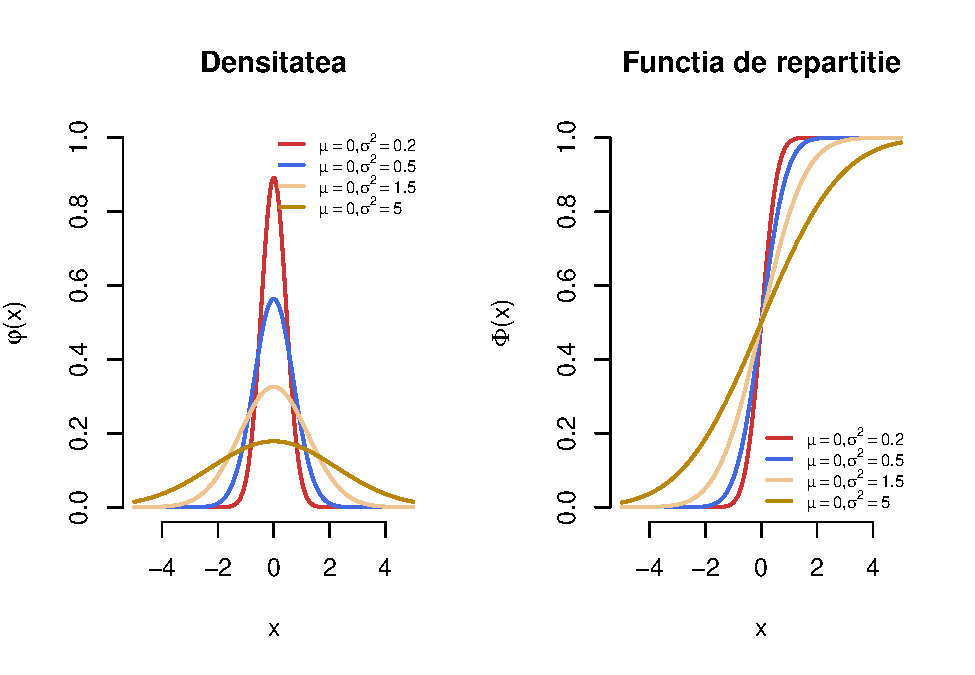
\includegraphics[width=0.7\linewidth]{Lab_1_files/figure-latex/unnamed-chunk-133-1} \end{center}

\begin{rmdexercise}
Generați \(250\) de observații din repartiția \(\mathcal{N}(0, 2)\),
trasați histograma acestora și suprapuneți densitatea repartiției date
(vezi figura de mai jos).
\end{rmdexercise}

\begin{center}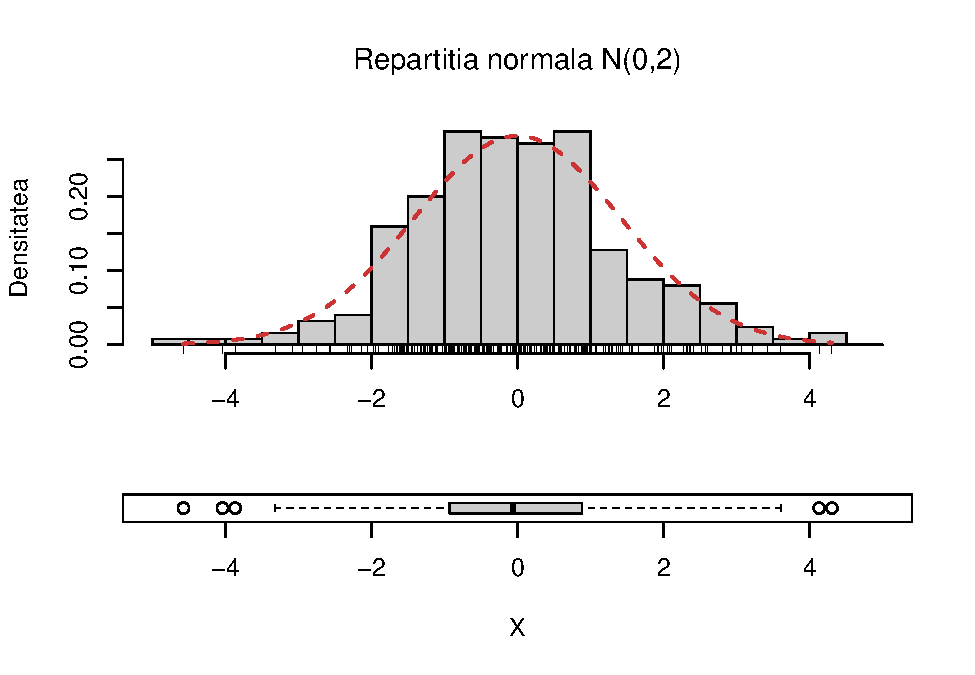
\includegraphics[width=0.7\linewidth]{Lab_1_files/figure-latex/unnamed-chunk-135-1} \end{center}

\begin{rmdexercise}
Fie \(X\) o variabilă aleatoare repartizată normal de parametrii \(\mu\)
și \(\sigma^2\). Ilustrați grafic pentru \(\mu = 0\) și \(\sigma = 1\)
că are loc următoarea inegalitate:

\[
  \left(\frac{1}{x}-\frac{1}{x^3}\right)\phi(x)<1-\Phi(x)<\frac{1}{x}\phi(x), \quad x>0.
\]
\end{rmdexercise}

\begin{center}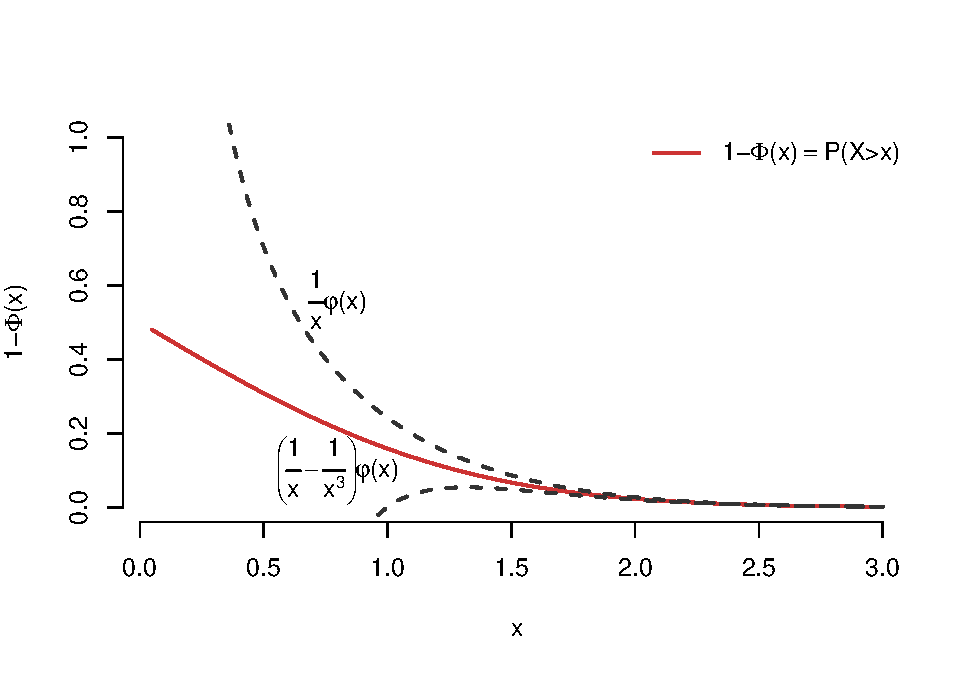
\includegraphics[width=0.7\linewidth]{Lab_1_files/figure-latex/unnamed-chunk-137-1} \end{center}

\subsection{Repartiția Log-Normală}\label{repartitia-log-normala}

Spune că o variabilă aleatoare \(X\) este repartizată log-normal de
parametrii \(\mu\) și \(\sigma^2\), și notăm
\(X\sim LN(\mu, \sigma^2)\), dacă \(\ln(X)\) este repartizată normal de
parametrii \(\mu\) și \(\sigma^2\). Cu alte cuvinte dacă
\(Y\sim \mathcal{N}(\mu, \sigma^2)\) atunci
\(X=e^Y\sim LN(\mu, \sigma^2)\). Densitatea repartiției log-normale
\(LN(\mu, \sigma^2)\) este

\[
    f_X(x) = \frac{1}{x\sigma\sqrt{2\pi}}e^{-\frac{(\ln(x)-\mu)^2}{2\sigma^2}}, \quad x\in (0, +\infty).
\]

\begin{center}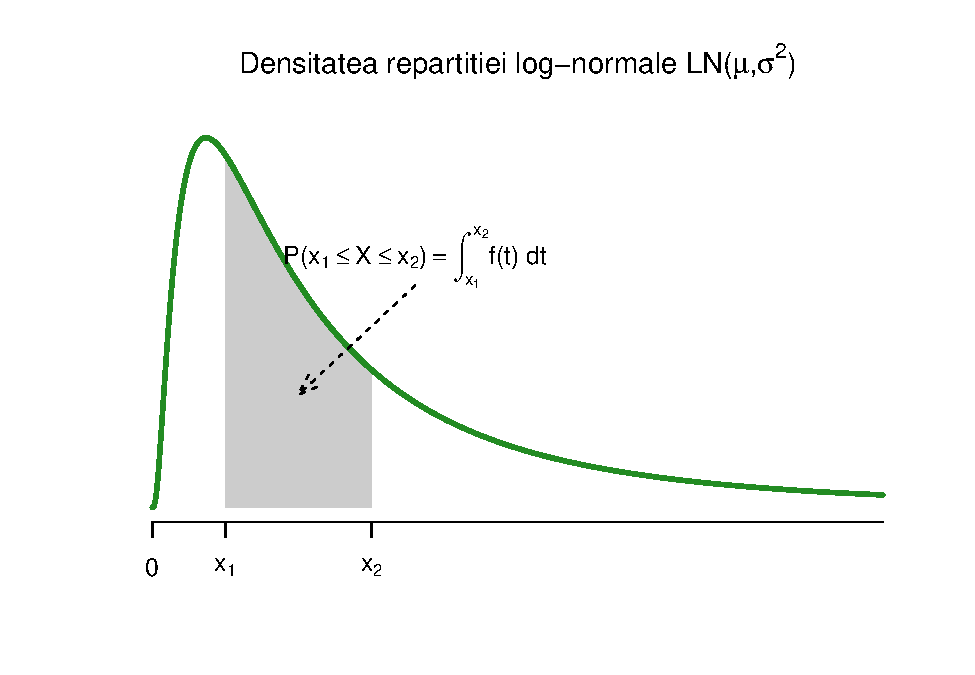
\includegraphics[width=0.7\linewidth]{Lab_1_files/figure-latex/unnamed-chunk-138-1} \end{center}

Funcția de repartiție a unei variabile aleatoare
\(X\sim LN(\mu, \sigma^2)\) este dată de

\[
  F_{X}(x) = \int_{-\infty}^{x}f_X(t)\,dt = \frac{1}{\sqrt{2\pi}\sigma}\int_{-\infty}^{x}\frac{1}{t}e^{-\frac{(\ln(t)-\mu)^2}{2\sigma^2}}\,dt
\]

și, ca și în cazul repartiției normale, nu are o formulă explicită de
calcul.

\begin{center}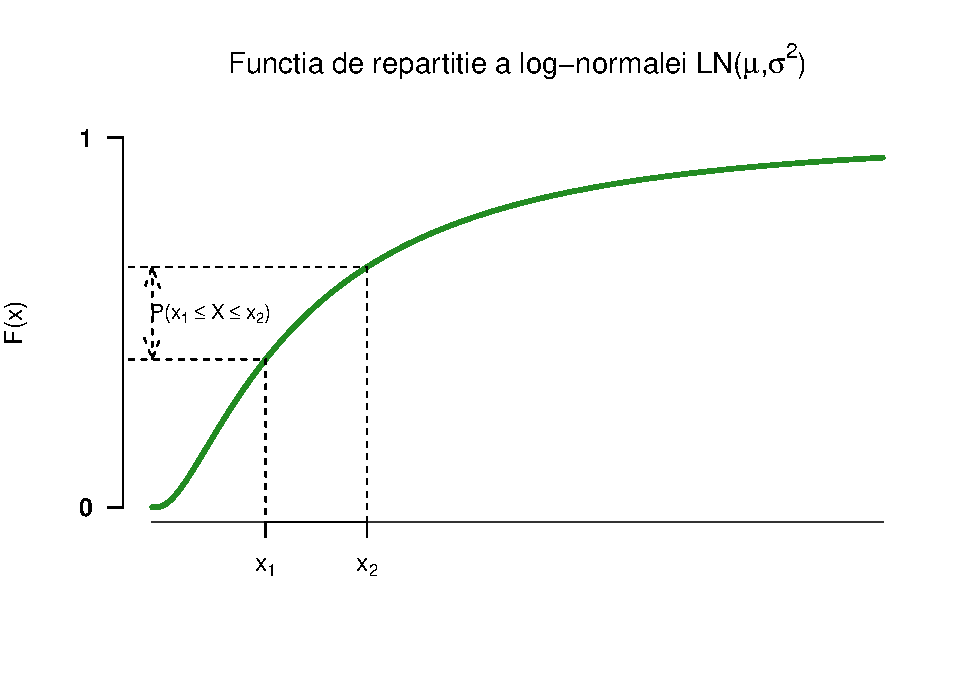
\includegraphics[width=0.7\linewidth]{Lab_1_files/figure-latex/unnamed-chunk-139-1} \end{center}

Media și varianța variabilei aleatoare \(X\) repartizate log-normal de
parametrii \(LN(\mu, \sigma^2)\) sunt egale cu

\[
  \mathbb{E}[X] = e^{\mu+\frac{\sigma^2}{2}},\quad Var(X) = \left(e^{\sigma^2}-1\right)e^{2\mu+\sigma^2}. 
\]

\begin{rmdexercise}
Arătați că media și varianța unei variabile aleatoare repartizate
log-normal de parametrii \(\mu\) și \(\sigma^2\) sunt egale cu

\[
  \mathbb{E}[X] = e^{\mu+\frac{\sigma^2}{2}},\quad Var(X) = \left(e^{\sigma^2}-1\right)e^{2\mu+\sigma^2}. 
\]
\end{rmdexercise}

În R putem să

\begin{itemize}
\tightlist
\item
  generăm observații independente din repartiția \(LN(\mu, \sigma^2)\)
  (e.g. \(\mu = 0\) și \(\sigma^2 = 3\) - ca și în cazul repartiției
  normale, funcțiile \texttt{rlnorm}, \texttt{dlnorm}, \texttt{plnorm}
  și \texttt{qlnorm} primesc ca parametrii media și abaterea standard,
  \(\sigma\) pentru \(\ln(X)\) - variabila normală)
\end{itemize}

\begin{Shaded}
\begin{Highlighting}[]
\KeywordTok{rlnorm}\NormalTok{(}\DecValTok{15}\NormalTok{, }\DataTypeTok{meanlog =} \DecValTok{0}\NormalTok{, }\DataTypeTok{sdlog =} \KeywordTok{sqrt}\NormalTok{(}\DecValTok{3}\NormalTok{))}
\NormalTok{ [}\DecValTok{1}\NormalTok{]  }\FloatTok{2.13141475}  \FloatTok{6.27258447}  \FloatTok{2.18850080}  \FloatTok{3.15407005}  \FloatTok{0.13970018}
\NormalTok{ [}\DecValTok{6}\NormalTok{]  }\FloatTok{0.52638598} \FloatTok{12.91237780}  \FloatTok{0.12004802}  \FloatTok{1.56359485}  \FloatTok{2.01674623}
\NormalTok{[}\DecValTok{11}\NormalTok{]  }\FloatTok{5.42024453}  \FloatTok{0.54647199}  \FloatTok{1.31619806}  \FloatTok{0.04716763}  \FloatTok{1.79762358}
\end{Highlighting}
\end{Shaded}

\begin{itemize}
\tightlist
\item
  calculăm densitatea unei variabile aleatoare repartizate log-normal
  \(LN(\mu, \sigma^2)\) în diferite puncte
\end{itemize}

\begin{Shaded}
\begin{Highlighting}[]
\KeywordTok{dlnorm}\NormalTok{(}\KeywordTok{seq}\NormalTok{(}\DecValTok{0}\NormalTok{, }\DecValTok{5}\NormalTok{, }\DataTypeTok{length.out =} \DecValTok{20}\NormalTok{), }\DataTypeTok{meanlog =} \DecValTok{3}\NormalTok{, }\DataTypeTok{sdlog =} \DecValTok{5}\NormalTok{)}
\NormalTok{ [}\DecValTok{1}\NormalTok{] }\FloatTok{0.00000000} \FloatTok{0.20820751} \FloatTok{0.11627647} \FloatTok{0.08196427} \FloatTok{0.06370023} \FloatTok{0.05226715}
\NormalTok{ [}\DecValTok{7}\NormalTok{] }\FloatTok{0.04440086} \FloatTok{0.03864103} \FloatTok{0.03423291} \FloatTok{0.03074580} \FloatTok{0.02791546} \FloatTok{0.02557044}
\NormalTok{[}\DecValTok{13}\NormalTok{] }\FloatTok{0.02359456} \FloatTok{0.02190618} \FloatTok{0.02044622} \FloatTok{0.01917084} \FloatTok{0.01804680} \FloatTok{0.01704845}
\NormalTok{[}\DecValTok{19}\NormalTok{] }\FloatTok{0.01615564} \FloatTok{0.01535234}
\end{Highlighting}
\end{Shaded}

\begin{itemize}
\tightlist
\item
  calculăm funcția de repartiție a unei variabile repartizate log-normal
  \(LN(\mu, \sigma^2)\) pentru diferite valori
\end{itemize}

\begin{Shaded}
\begin{Highlighting}[]
\KeywordTok{plnorm}\NormalTok{(}\KeywordTok{seq}\NormalTok{(}\DecValTok{0}\NormalTok{, }\DecValTok{15}\NormalTok{, }\DataTypeTok{length.out =} \DecValTok{25}\NormalTok{), }\DataTypeTok{meanlog =} \DecValTok{3}\NormalTok{, }\DataTypeTok{sdlog =} \DecValTok{1}\NormalTok{)}
\NormalTok{ [}\DecValTok{1}\NormalTok{] }\FloatTok{0.0000000000} \FloatTok{0.0002602257} \FloatTok{0.0027443707} \FloatTok{0.0088606283} \FloatTok{0.0185933103}
\NormalTok{ [}\DecValTok{6}\NormalTok{] }\FloatTok{0.0314027650} \FloatTok{0.0466497221} \FloatTok{0.0637426806} \FloatTok{0.0821791298} \FloatTok{0.1015482283}
\NormalTok{[}\DecValTok{11}\NormalTok{] }\FloatTok{0.1215206945} \FloatTok{0.1418356830} \FloatTok{0.1622882185} \FloatTok{0.1827183180} \FloatTok{0.2030019832}
\NormalTok{[}\DecValTok{16}\NormalTok{] }\FloatTok{0.2230439002} \FloatTok{0.2427715876} \FloatTok{0.2621307274} \FloatTok{0.2810814477} \FloatTok{0.2995953616}
\NormalTok{[}\DecValTok{21}\NormalTok{] }\FloatTok{0.3176532076} \FloatTok{0.3352429649} \FloatTok{0.3523583472} \FloatTok{0.3689975944} \FloatTok{0.3851625036}
\end{Highlighting}
\end{Shaded}

\begin{itemize}
\tightlist
\item
  calculăm cuantilele de ordin \(\alpha\in(0,1)\)
\end{itemize}

\begin{Shaded}
\begin{Highlighting}[]
\KeywordTok{qlnorm}\NormalTok{(}\KeywordTok{c}\NormalTok{(}\FloatTok{0.01}\NormalTok{, }\FloatTok{0.025}\NormalTok{, }\FloatTok{0.05}\NormalTok{, }\FloatTok{0.25}\NormalTok{, }\FloatTok{0.5}\NormalTok{, }\FloatTok{0.75}\NormalTok{, }\FloatTok{0.95}\NormalTok{, }\FloatTok{0.975}\NormalTok{, }\FloatTok{0.99}\NormalTok{), }\DataTypeTok{meanlog =} \DecValTok{0}\NormalTok{, }\DataTypeTok{sdlog =} \DecValTok{1}\NormalTok{)}
\NormalTok{[}\DecValTok{1}\NormalTok{]  }\FloatTok{0.09765173}  \FloatTok{0.14086349}  \FloatTok{0.19304082}  \FloatTok{0.50941628}  \FloatTok{1.00000000}  \FloatTok{1.96303108}
\NormalTok{[}\DecValTok{7}\NormalTok{]  }\FloatTok{5.18025160}  \FloatTok{7.09907138} \FloatTok{10.24047366}
\end{Highlighting}
\end{Shaded}

\begin{rmdexercise}
Fie \(X\) o variabilă aleatoare repartizată \(LN(\mu, \sigma^2)\).
Pentru \(\mu = 0\) și \(\sigma \in \{0.25, 0.5, 1.5, 5\}\) trasați pe
același grafic densitățile repartițiilor log-normale cu parametrii
\(LN(\mu, \sigma^2)\). Adăugați legendele corespunzătoare. Aceeași
cerință pentru funcțiile de repartiție.
\end{rmdexercise}

\begin{center}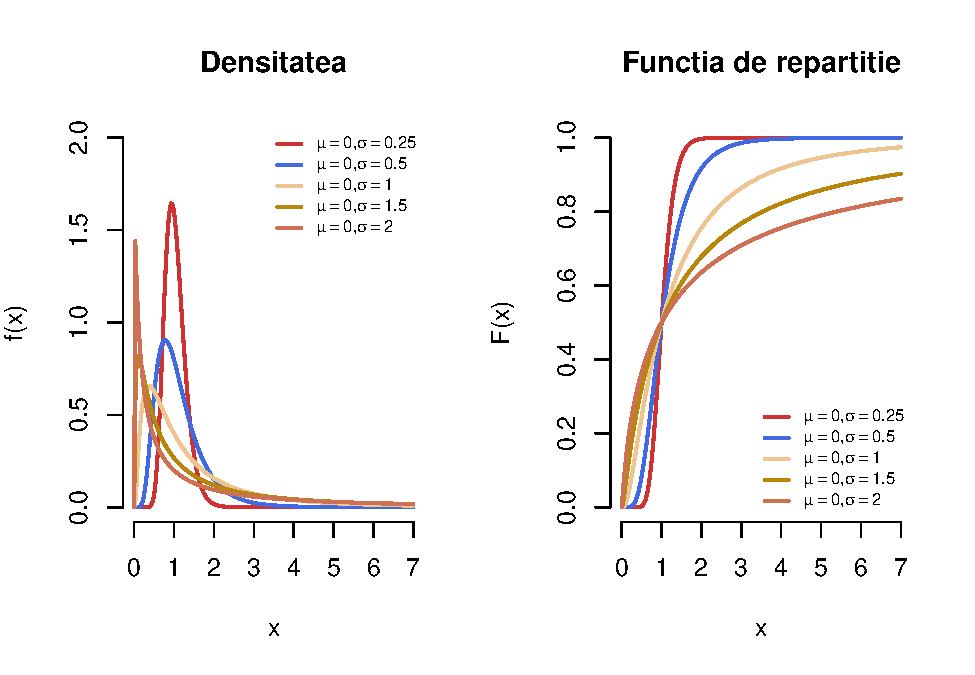
\includegraphics[width=0.7\linewidth]{Lab_1_files/figure-latex/unnamed-chunk-146-1} \end{center}

\begin{rmdexercise}
Generați \(500\) de observații din repartiția \(LN(0, 2)\), trasați
histograma acestora și suprapuneți densitatea repartiției date (vezi
figura de mai jos).
\end{rmdexercise}

\begin{center}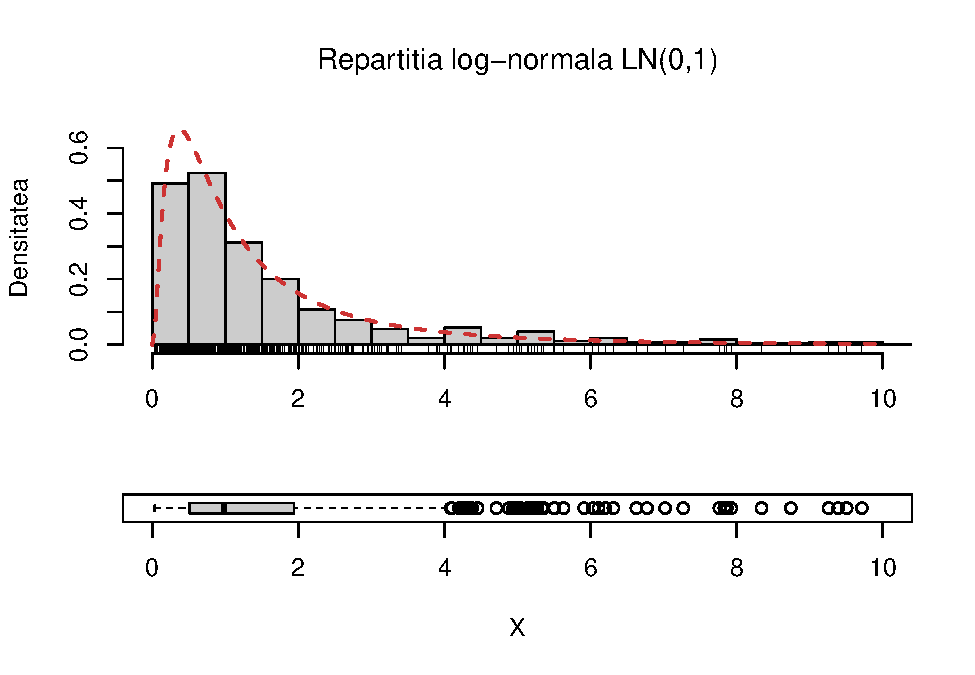
\includegraphics[width=0.7\linewidth]{Lab_1_files/figure-latex/unnamed-chunk-148-1} \end{center}

Printre fenomenele care pot fi modelate cu ajutorul repartiției
log-normale se numără: cantitatea de lapte produsă de vaci, cantitatea
de ploaie dintr-o perioadă dată, repartiția mărimii picăturilor de
ploaie, volumul de gaz dintr-o rezervă petrolieră, etc. Pentru mai multe
aplicații se poate consulta lucrarea lui Limpert, E., Stajel, W. și
Abbt, M.
\href{http://stat.ethz.ch/~stahel/lognormal/bioscience.pdf}{Log-normal
Distributions across the Sciences: Keys and Clues}, \emph{BioScience},
Vol. 51, Nr. 5, 2001.

\subsection{Repartiția Exponențială}\label{repartitia-exponentiala}

Spunem că o variabilă aleatoare \(X\) este repartizată
\emph{exponențial} de parametru \(\lambda\), și se notează cu
\(X\sim\mathcal{E}(\lambda)\), dacă densitatea ei are forma

\[
  f_X(x) = \lambda e^{-\lambda x}\mathbb{1}_{\mathbb{R}_+}(x),\quad \forall x\in\mathbb{R}.
\]

\begin{center}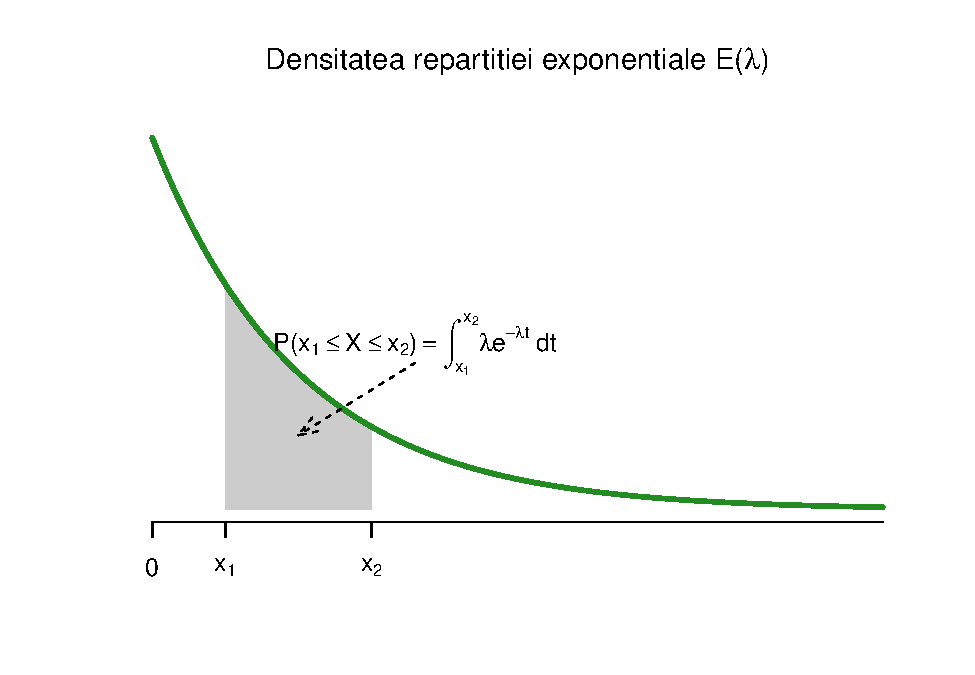
\includegraphics[width=0.7\linewidth]{Lab_1_files/figure-latex/unnamed-chunk-149-1} \end{center}

Funcția de repartiție a unei variabile aleatoare
\(X\sim \mathcal{E}(\lambda)\) este dată de

\[
  F_{X}(x) = 1 - e^{-\lambda x}\mathbb{1}_{\mathbb{R}_+}(x), \quad x\in \mathbb{R}.
\]

\begin{center}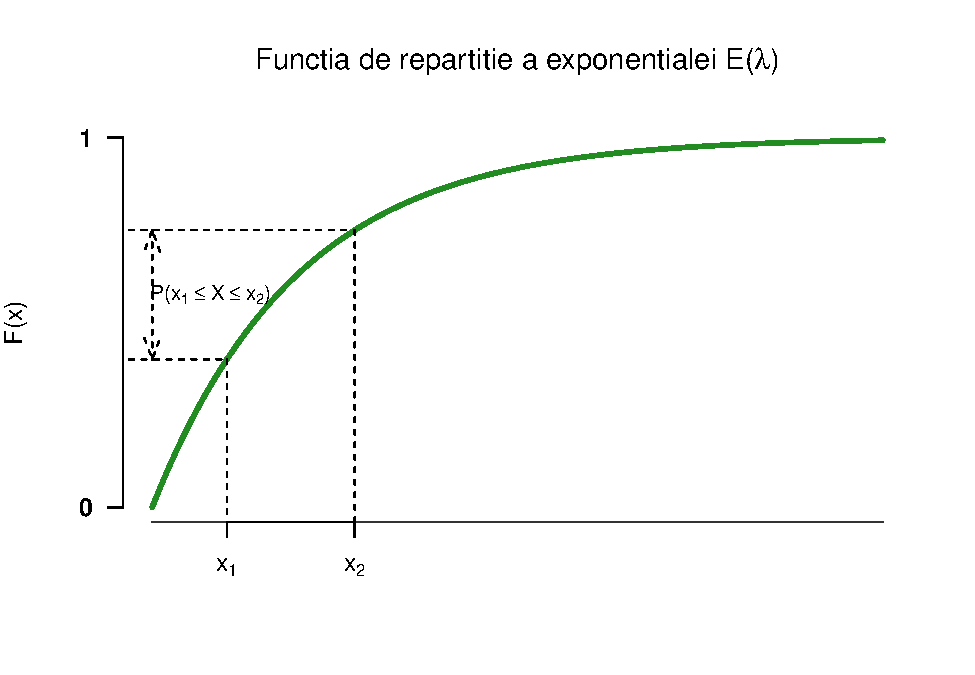
\includegraphics[width=0.7\linewidth]{Lab_1_files/figure-latex/unnamed-chunk-150-1} \end{center}

Media și varianța variabilei aleatoare \(X\) repartizate exponențial de
parametru \(\lambda\) sunt egale cu

\[
  \mathbb{E}[X] = \frac{1}{\lambda},\quad Var(X) =  \frac{1}{\lambda^2}. 
\]

\begin{rmdexercise}
Arătați că momentul de ordin \(k\), \(k\geq 1\), al unei variabile
aleatoare repartizate exponențial \(X\sim\mathcal{E}(\lambda)\) este
egal cu

\[
  \mathbb{E}[X^k] = \frac{k!}{\lambda^k}. 
\]
\end{rmdexercise}

\begin{rmdinsight}
Fie \(X\) o variabilă repartizată exponențial de parametru \(\lambda\).
Atunci are loc următoarea proprietate numită și \emph{lipsa de memorie}:

\[
      \mathbb{P}(X>s+t|X>s) = \mathbb{P}(X>t),\quad \forall s,t \geq 0. 
\]

Mai mult, dacă o variabilă aleatoare continuă\footnote{Pentru cazul
  discret avem variabila repartizată Geometric.} \(X\) verifică
proprietatea de mai sus atunci ea este repartizată exponențial.
\end{rmdinsight}

Variabilele aleatoare repartizate exponențial sunt utilizate în
modelarea fenomenelor care se desfășoară în timp continuu și care
satisfac (aproximativ) proprietatea lipsei de memorie: de exemplu timpul
de așteptare la un ghișeu, durata de viață a unui bec sau timpul până la
următoarea convorbire telefonică.

În R putem să

\begin{itemize}
\tightlist
\item
  generăm observații independente din repartiția
  \(\mathcal{E}(\lambda)\) (e.g. \(\lambda = 5\))
\end{itemize}

\begin{Shaded}
\begin{Highlighting}[]
\KeywordTok{rexp}\NormalTok{(}\DecValTok{15}\NormalTok{, }\DataTypeTok{rate =} \DecValTok{5}\NormalTok{)}
\NormalTok{ [}\DecValTok{1}\NormalTok{] }\FloatTok{0.13505357} \FloatTok{0.15392539} \FloatTok{0.25036131} \FloatTok{0.15351051} \FloatTok{0.00878456} \FloatTok{0.07362396}
\NormalTok{ [}\DecValTok{7}\NormalTok{] }\FloatTok{0.07543271} \FloatTok{0.18981181} \FloatTok{0.05540771} \FloatTok{0.05649451} \FloatTok{0.15878039} \FloatTok{0.39847262}
\NormalTok{[}\DecValTok{13}\NormalTok{] }\FloatTok{0.05191221} \FloatTok{0.07776034} \FloatTok{0.22483594}
\end{Highlighting}
\end{Shaded}

\begin{itemize}
\tightlist
\item
  calculăm densitatea unei variabile aleatoare repartizate exponențial
  \(\mathcal{E}(\lambda)\) în diferite puncte
\end{itemize}

\begin{Shaded}
\begin{Highlighting}[]
\KeywordTok{dexp}\NormalTok{(}\KeywordTok{seq}\NormalTok{(}\DecValTok{0}\NormalTok{, }\DecValTok{5}\NormalTok{, }\DataTypeTok{length.out =} \DecValTok{20}\NormalTok{), }\DataTypeTok{rate =} \DecValTok{5}\NormalTok{)}
\NormalTok{ [}\DecValTok{1}\NormalTok{] }\FloatTok{5.000000e+00} \FloatTok{1.341312e+00} \FloatTok{3.598237e-01} \FloatTok{9.652719e-02} \FloatTok{2.589462e-02}
\NormalTok{ [}\DecValTok{6}\NormalTok{] }\FloatTok{6.946555e-03} \FloatTok{1.863500e-03} \FloatTok{4.999070e-04} \FloatTok{1.341063e-04} \FloatTok{3.597568e-05}
\NormalTok{[}\DecValTok{11}\NormalTok{] }\FloatTok{9.650925e-06} \FloatTok{2.588981e-06} \FloatTok{6.945263e-07} \FloatTok{1.863153e-07} \FloatTok{4.998141e-08}
\NormalTok{[}\DecValTok{16}\NormalTok{] }\FloatTok{1.340814e-08} \FloatTok{3.596899e-09} \FloatTok{9.649130e-10} \FloatTok{2.588499e-10} \FloatTok{6.943972e-11}
\end{Highlighting}
\end{Shaded}

\begin{itemize}
\tightlist
\item
  calculăm funcția de repartiție a unei variabile repartizate
  exponențial \(\mathcal{E}(\lambda)\) pentru diferite valori
\end{itemize}

\begin{Shaded}
\begin{Highlighting}[]
\KeywordTok{pexp}\NormalTok{(}\KeywordTok{seq}\NormalTok{(}\DecValTok{0}\NormalTok{, }\DecValTok{5}\NormalTok{, }\DataTypeTok{length.out =} \DecValTok{15}\NormalTok{), }\DataTypeTok{rate =} \DecValTok{5}\NormalTok{)}
\NormalTok{ [}\DecValTok{1}\NormalTok{] }\FloatTok{0.0000000} \FloatTok{0.8323228} \FloatTok{0.9718843} \FloatTok{0.9952856} \FloatTok{0.9992095} \FloatTok{0.9998675} \FloatTok{0.9999778}
\NormalTok{ [}\DecValTok{8}\NormalTok{] }\FloatTok{0.9999963} \FloatTok{0.9999994} \FloatTok{0.9999999} \FloatTok{1.0000000} \FloatTok{1.0000000} \FloatTok{1.0000000} \FloatTok{1.0000000}
\NormalTok{[}\DecValTok{15}\NormalTok{] }\FloatTok{1.0000000}
\end{Highlighting}
\end{Shaded}

\begin{itemize}
\tightlist
\item
  calculăm cuantilele de ordin \(\alpha\in(0,1)\)
\end{itemize}

\begin{Shaded}
\begin{Highlighting}[]
\KeywordTok{qexp}\NormalTok{(}\KeywordTok{c}\NormalTok{(}\FloatTok{0.01}\NormalTok{, }\FloatTok{0.025}\NormalTok{, }\FloatTok{0.05}\NormalTok{, }\FloatTok{0.25}\NormalTok{, }\FloatTok{0.5}\NormalTok{, }\FloatTok{0.75}\NormalTok{, }\FloatTok{0.95}\NormalTok{, }\FloatTok{0.975}\NormalTok{, }\FloatTok{0.99}\NormalTok{), }\DataTypeTok{rate =} \DecValTok{5}\NormalTok{)}
\NormalTok{[}\DecValTok{1}\NormalTok{] }\FloatTok{0.002010067} \FloatTok{0.005063562} \FloatTok{0.010258659} \FloatTok{0.057536414} \FloatTok{0.138629436} \FloatTok{0.277258872}
\NormalTok{[}\DecValTok{7}\NormalTok{] }\FloatTok{0.599146455} \FloatTok{0.737775891} \FloatTok{0.921034037}
\end{Highlighting}
\end{Shaded}

\begin{rmdexercise}
Fie \(X\) o variabilă aleatoare repartizată \(\mathcal{E}(\lambda)\).
Pentru \(\lambda \in \{0.5, 1.5, 5\}\) trasați pe același grafic
densitățile repartițiilor exponențiale de parametru \(\lambda\).
Adăugați legendele corespunzătoare. Aceeași cerință pentru funcțiile de
repartiție.
\end{rmdexercise}

\begin{center}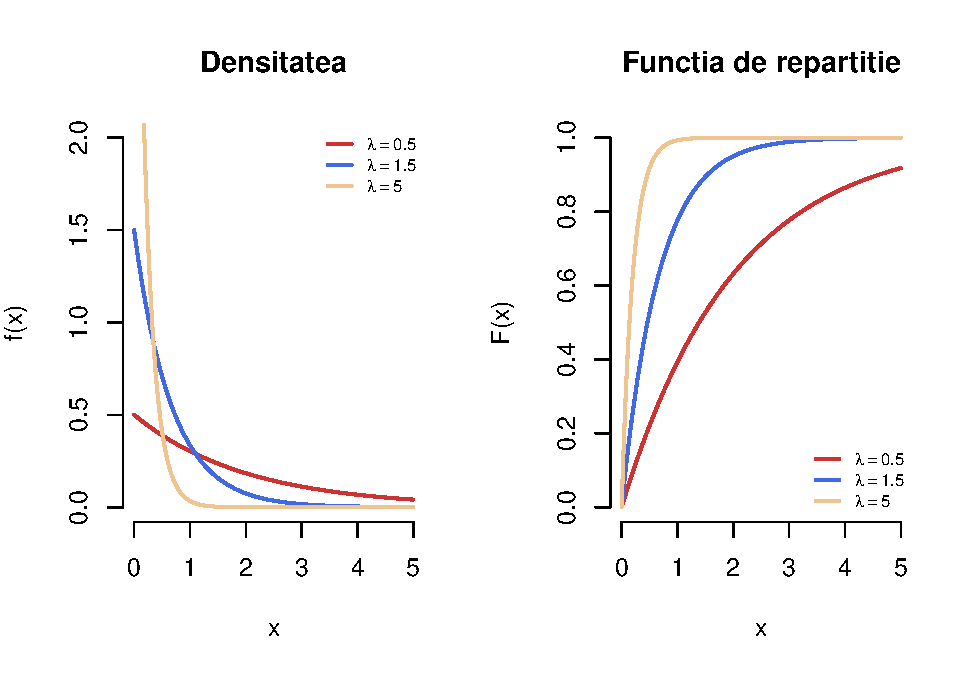
\includegraphics[width=0.7\linewidth]{Lab_1_files/figure-latex/unnamed-chunk-158-1} \end{center}

\begin{rmdexercise}
Folosind rezultatul de universalitate de la repartiția uniformă,
descrieți o procedură prin care puteți simula o variabilă aleatoare
repartizată exponențial \(\mathcal{E}(\lambda)\) și construiți o funcție
care permite generarea de \(n\) observații independente dintr-o
variabilă repartizată \(X\sim \mathcal{E}(\lambda)\).
\end{rmdexercise}

\begin{rmdexercise}
Generați \(250\) de observații din repartiția \(\mathcal{E}(3)\),
trasați histograma acestora și suprapuneți densitatea repartiției date
(vezi figura de mai jos).
\end{rmdexercise}

\begin{center}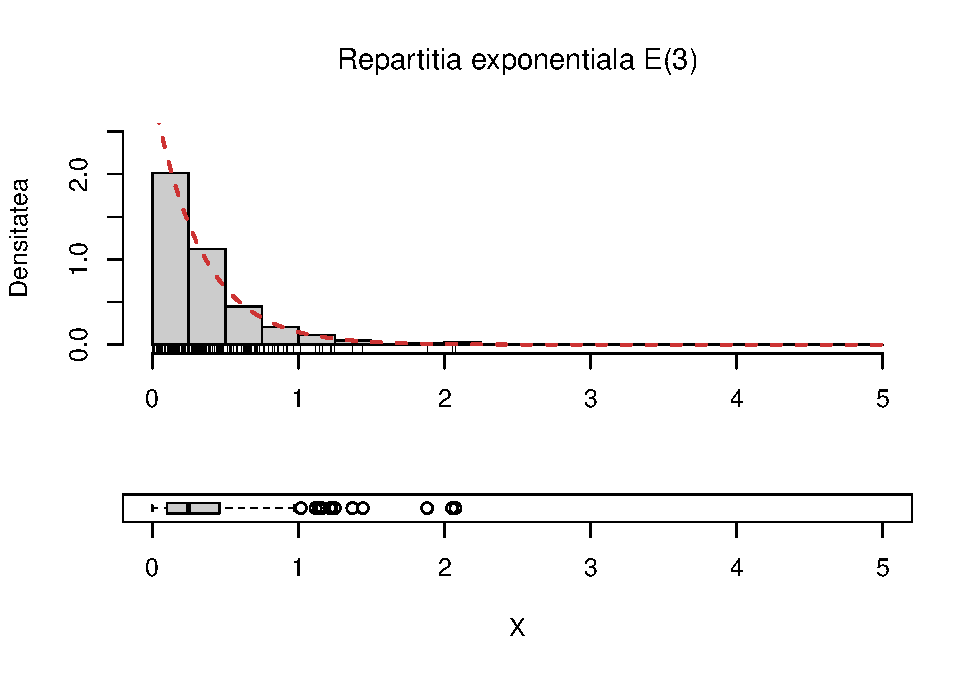
\includegraphics[width=0.7\linewidth]{Lab_1_files/figure-latex/unnamed-chunk-162-1} \end{center}

\subsection{Repartiția Cauchy}\label{repartitia-cauchy}

Spunem că o variabilă aleatoare \(X\) este repartizată \emph{Cauchy} de
parametrii \((0, 1)\), și se notează cu \(X\sim C(0,1)\), dacă
densitatea ei are forma

\[
  f_X(x) = \frac{1}{\pi} \frac{1}{1+x^2},\quad \forall x\in\mathbb{R}.
\]

Observăm că graficul densității repartiției Cauchy este asemănător cu
cel al repartiției normale. Parametrul \(M = 0\) reprezintă mediana (de
fapt \(\mathbb{P}(X\leq 0) = \mathbb{P}(X\geq 0) = \frac{1}{2}\))
variabilei aleatoare \(X\) și nu media iar prima și a treia cuartilă
sunt \(Q_1 = -1\) și respectiv \(Q_3=1\) (avem
\(\mathbb{P}(X\leq -1) = \mathbb{P}(X\geq 1) = \frac{1}{4}\)).

\begin{center}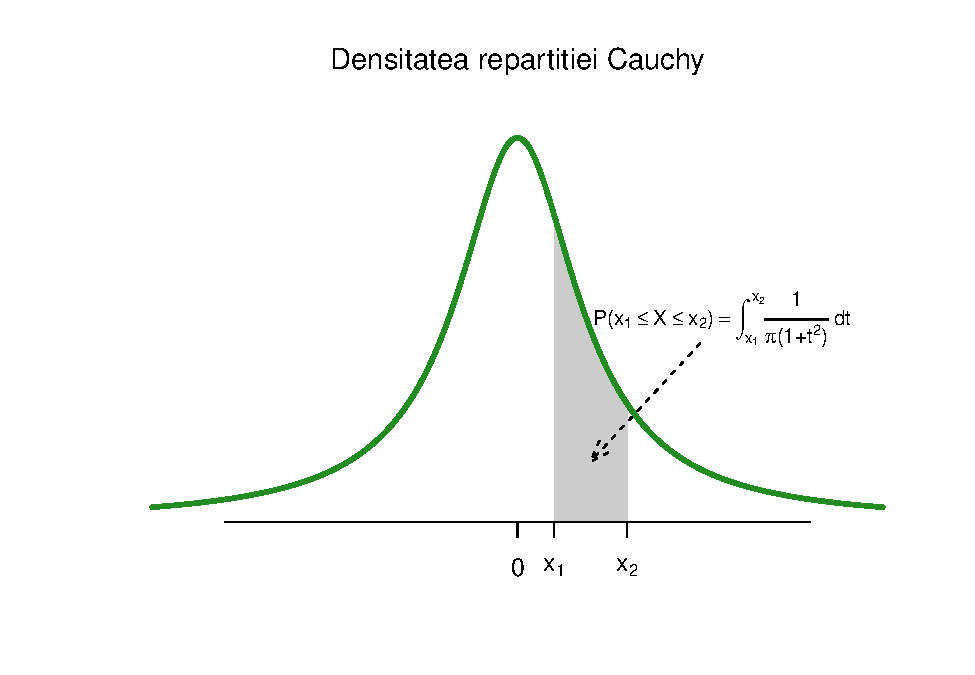
\includegraphics[width=0.7\linewidth]{Lab_1_files/figure-latex/unnamed-chunk-163-1} \end{center}

Funcția de repartiție a unei variabile aleatoare \(X\sim C(0,1)\) este
dată de

\[
  F_{X}(x) = \frac{1}{2} + \frac{1}{\pi}\arctan(x), \quad x\in \mathbb{R}.
\]

\begin{center}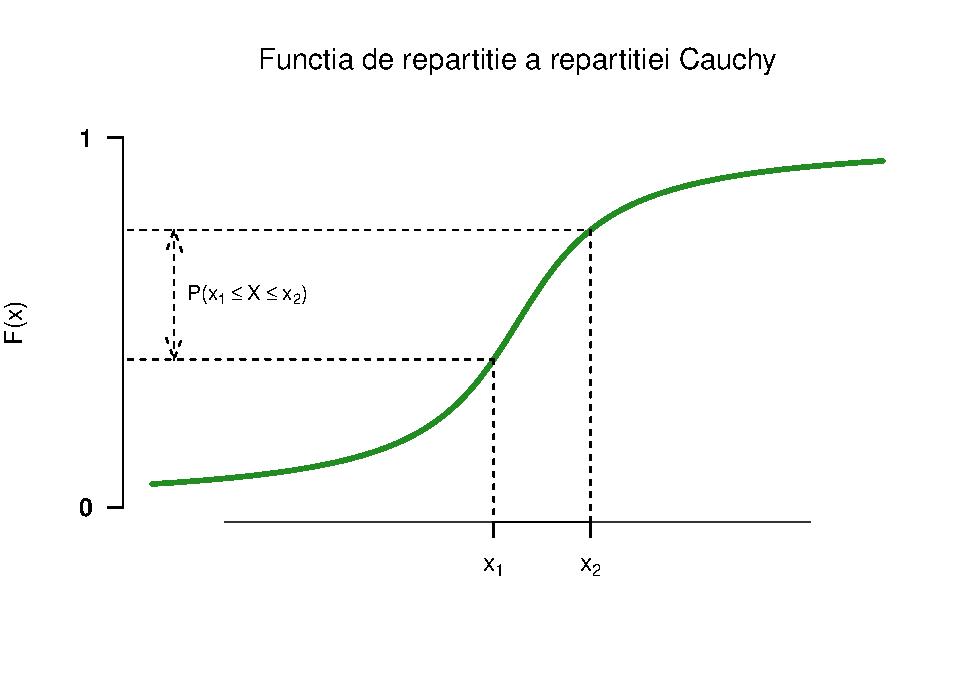
\includegraphics[width=0.7\linewidth]{Lab_1_files/figure-latex/unnamed-chunk-164-1} \end{center}

Media și varianța variabilei aleatoare \(X\sim C(0,1)\) \textbf{nu
există}.

\begin{rmdexercise}
Arătați că o variabilă aleatoare repartizată Cauchy \(C(0,1)\) nu are
medie.
\end{rmdexercise}

Fie \(Y\sim C(0,1)\) și \(\alpha, \beta\in\mathbb{R}\) cu \(\beta>0\).
Spunem că variabila aleatoare \(X = \alpha + \beta Y\) este repartizată
Cauchy de parametrii \((\alpha, \beta)\), \(X\sim C(\alpha, \beta)\).
Densitatea ei este

\[
  f_X(x) = \frac{1}{\pi\beta} \frac{1}{1+\left(\frac{x-\alpha}{\beta}\right)^2},\quad \forall x\in\mathbb{R}.
\]

Parametrii \(\alpha\) și \(\beta\) se interpretează în modul următor:
\(M = \alpha\) este mediana lui \(X\) iar \(Q_1 = \alpha-\beta\) și
\(Q_3 = \alpha + \beta\) reprezintă prima și a treia cuartilă.

În R putem să

\begin{itemize}
\tightlist
\item
  generăm observații independente din repartiția Cauchy
  \(C(\alpha, \beta)\) (e.g. \(\alpha = 0\), \(\beta = 2\))
\end{itemize}

\begin{Shaded}
\begin{Highlighting}[]
\KeywordTok{rcauchy}\NormalTok{(}\DecValTok{15}\NormalTok{, }\DataTypeTok{location =} \DecValTok{0}\NormalTok{, }\DataTypeTok{scale =} \DecValTok{2}\NormalTok{)}
\NormalTok{ [}\DecValTok{1}\NormalTok{] }\OperatorTok{-}\FloatTok{0.5966228}  \FloatTok{3.7627987}  \FloatTok{0.6864597} \OperatorTok{-}\FloatTok{0.4316018}  \FloatTok{1.4524446}  \FloatTok{0.3427032}
\NormalTok{ [}\DecValTok{7}\NormalTok{]  }\FloatTok{8.4285326}  \FloatTok{3.6056089}  \FloatTok{2.3506764} \OperatorTok{-}\FloatTok{3.5453329} \OperatorTok{-}\FloatTok{1.6137218} \FloatTok{10.4304800}
\NormalTok{[}\DecValTok{13}\NormalTok{] }\OperatorTok{-}\FloatTok{0.4449169}  \FloatTok{2.3005176} \OperatorTok{-}\FloatTok{3.6644199}
\end{Highlighting}
\end{Shaded}

\begin{itemize}
\tightlist
\item
  calculăm densitatea unei variabile aleatoare repartizate Cauchy
  \(C(\alpha, \beta)\) în diferite puncte
\end{itemize}

\begin{Shaded}
\begin{Highlighting}[]
\KeywordTok{dcauchy}\NormalTok{(}\KeywordTok{seq}\NormalTok{(}\OperatorTok{-}\DecValTok{5}\NormalTok{, }\DecValTok{5}\NormalTok{, }\DataTypeTok{length.out =} \DecValTok{20}\NormalTok{), }\DataTypeTok{location =} \DecValTok{1}\NormalTok{, }\DataTypeTok{scale =} \DecValTok{3}\NormalTok{)}
\NormalTok{ [}\DecValTok{1}\NormalTok{] }\FloatTok{0.02122066} \FloatTok{0.02450975} \FloatTok{0.02852541} \FloatTok{0.03345265} \FloatTok{0.03951056} \FloatTok{0.04693392}
\NormalTok{ [}\DecValTok{7}\NormalTok{] }\FloatTok{0.05591721} \FloatTok{0.06648594} \FloatTok{0.07825871} \FloatTok{0.09012539} \FloatTok{0.10006665} \FloatTok{0.10558334}
\NormalTok{[}\DecValTok{13}\NormalTok{] }\FloatTok{0.10494052} \FloatTok{0.09835367} \FloatTok{0.08782920} \FloatTok{0.07584810} \FloatTok{0.06425529} \FloatTok{0.05399054}
\NormalTok{[}\DecValTok{19}\NormalTok{] }\FloatTok{0.04532934} \FloatTok{0.03819719}
\end{Highlighting}
\end{Shaded}

\begin{itemize}
\tightlist
\item
  calculăm funcția de repartiție a unei variabile repartizate Cauchy
  \(C(\alpha, \beta)\) pentru diferite valori
\end{itemize}

\begin{Shaded}
\begin{Highlighting}[]
\KeywordTok{pcauchy}\NormalTok{(}\KeywordTok{seq}\NormalTok{(}\OperatorTok{-}\DecValTok{5}\NormalTok{, }\DecValTok{5}\NormalTok{, }\DataTypeTok{length.out =} \DecValTok{15}\NormalTok{), }\DataTypeTok{location =} \DecValTok{1}\NormalTok{, }\DataTypeTok{scale =} \DecValTok{3}\NormalTok{)}
\NormalTok{ [}\DecValTok{1}\NormalTok{] }\FloatTok{0.1475836} \FloatTok{0.1643213} \FloatTok{0.1848605} \FloatTok{0.2104166} \FloatTok{0.2425988} \FloatTok{0.2833834} \FloatTok{0.3347507}
\NormalTok{ [}\DecValTok{8}\NormalTok{] }\FloatTok{0.3975836} \FloatTok{0.4697759} \FloatTok{0.5451672} \FloatTok{0.6158581} \FloatTok{0.6764416} \FloatTok{0.7255627} \FloatTok{0.7644587}
\NormalTok{[}\DecValTok{15}\NormalTok{] }\FloatTok{0.7951672}
\end{Highlighting}
\end{Shaded}

\begin{itemize}
\tightlist
\item
  calculăm cuantilele de ordin \(p\in(0,1)\)
\end{itemize}

\begin{Shaded}
\begin{Highlighting}[]
\KeywordTok{qcauchy}\NormalTok{(}\KeywordTok{c}\NormalTok{(}\FloatTok{0.01}\NormalTok{, }\FloatTok{0.025}\NormalTok{, }\FloatTok{0.05}\NormalTok{, }\FloatTok{0.25}\NormalTok{, }\FloatTok{0.5}\NormalTok{, }\FloatTok{0.75}\NormalTok{, }\FloatTok{0.95}\NormalTok{, }\FloatTok{0.975}\NormalTok{, }\FloatTok{0.99}\NormalTok{), }\DataTypeTok{location =} \DecValTok{1}\NormalTok{, }\DataTypeTok{scale =} \DecValTok{3}\NormalTok{)}
\NormalTok{[}\DecValTok{1}\NormalTok{] }\OperatorTok{-}\FloatTok{94.46155} \OperatorTok{-}\FloatTok{37.11861} \OperatorTok{-}\FloatTok{17.94125}  \OperatorTok{-}\FloatTok{2.00000}   \FloatTok{1.00000}   \FloatTok{4.00000}  \FloatTok{19.94125}
\NormalTok{[}\DecValTok{8}\NormalTok{]  }\FloatTok{39.11861}  \FloatTok{96.46155}
\end{Highlighting}
\end{Shaded}

\begin{rmdexercise}
Generați \(2500\) de observații din repartiția Cauchy, trasați
histograma acestora și suprapuneți densitatea repartiției date pentru
intervalul \([-5,5]\) (vezi figura de mai jos).
\end{rmdexercise}

\begin{center}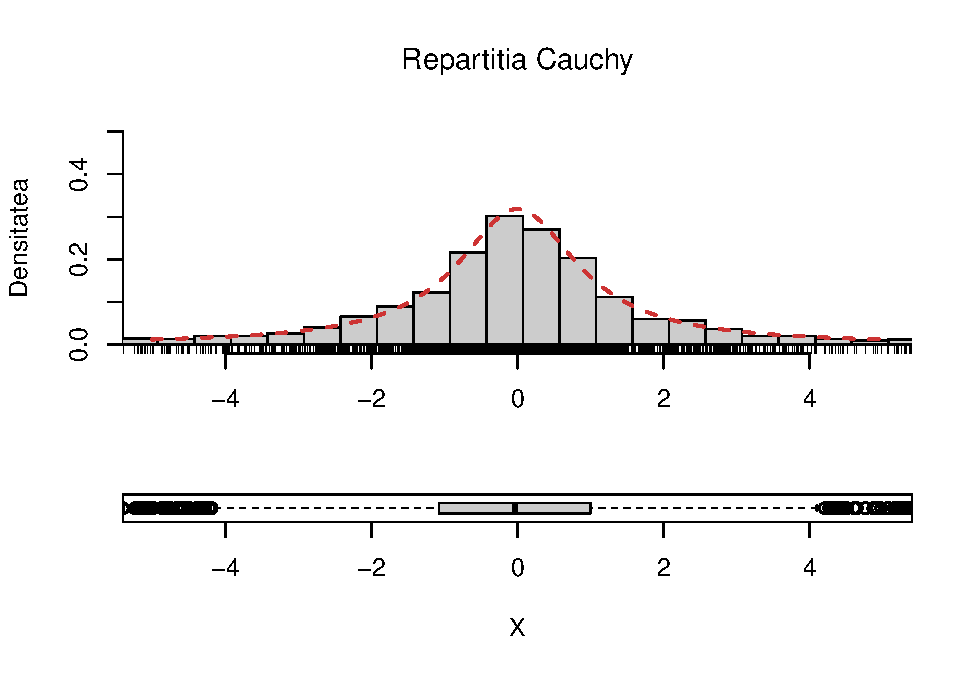
\includegraphics[width=0.7\linewidth]{Lab_1_files/figure-latex/unnamed-chunk-171-1} \end{center}

\begin{rmdexercise}
Fie \(X\) și \(Y\) două variabile aleatoare independente repartizate
\(\mathcal{N}(0,1)\). Arătați că variabila aleatoare \(\frac{X}{Y}\)
este repartizată Cauchy \(C(0,1)\).
\end{rmdexercise}

\begin{rmdexercise}
Fie \(X\) o variabilă aleatoare repartizată Cauchy \(C(\alpha, \beta)\).
Pentru fiecare pereche de parametrii \((\alpha, \beta)\) din mulțimea
\(\{(0,0.5), (0, 1), (0, 2), (-1, 1.5), (-2, 1)\}\) trasați pe același
grafic densitățile repartițiilor Cauchy cu parametrii
\((\alpha, \beta)\). Adăugați legendele corespunzătoare. Aceeași cerință
pentru funcțiile de repartiție.
\end{rmdexercise}

\begin{center}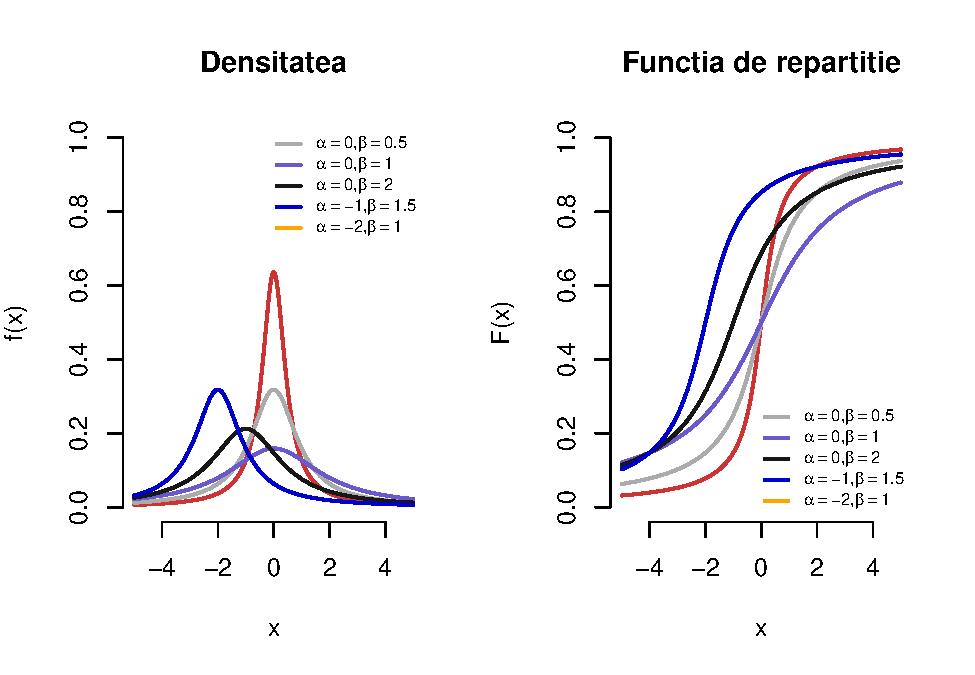
\includegraphics[width=0.7\linewidth]{Lab_1_files/figure-latex/unnamed-chunk-174-1} \end{center}

\begin{rmdexercise}
Folosind rezultatul de universalitate de la repartiția uniformă,
descrieți o procedură prin care puteți simula o variabilă aleatoare
repartizată Cauchy \(C(0,1)\) și construiți o funcție care permite
generarea de \(n\) observații independente dintr-o variabilă repartizată
\(X\sim C(\alpha, \beta)\). Verificați pentru parametrii \(\alpha = 3\)
și \(\beta = 5\) (a se vedea figura de mai jos).
\end{rmdexercise}

\begin{verbatim}
Warning in rug(x): some values will be clipped
\end{verbatim}

\begin{center}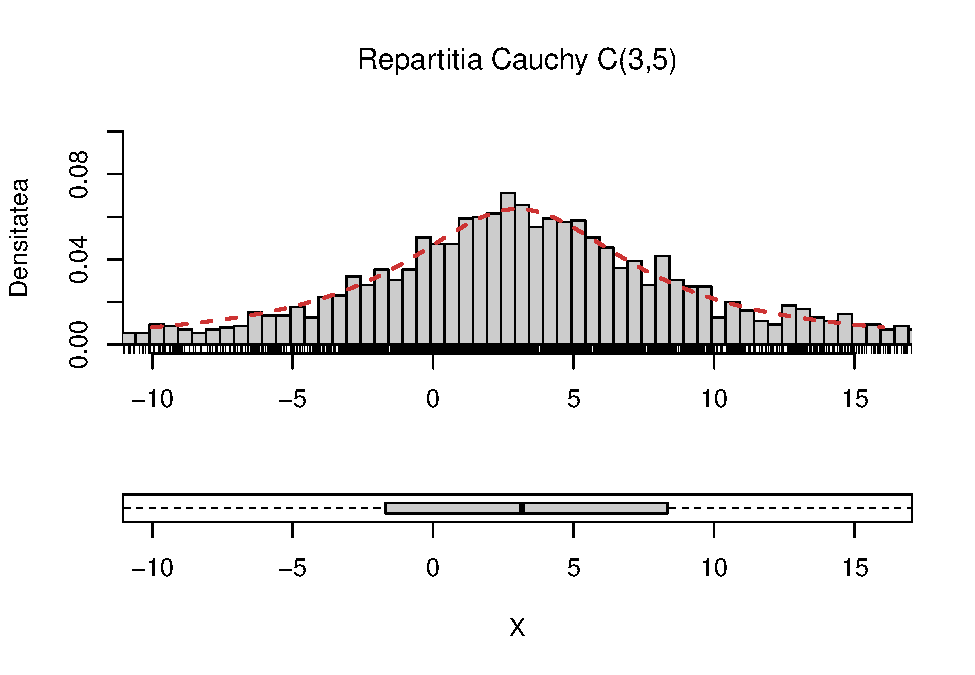
\includegraphics{Lab_1_files/figure-latex/unnamed-chunk-176-1} \end{center}

\subsection{Repartiția Gama}\label{repartitia-gama}

Spunem că o variabilă aleatoare \(X\) este repartizată \emph{Gama} de
parametrii \((\alpha, \beta)\), cu \(\alpha, \beta > 0\), și se notează
cu \(X\sim \Gamma(\alpha,\beta)\), dacă densitatea ei are forma

\[
  f_X(x) = \frac{\beta^{\alpha}}{\Gamma(\alpha)} x^{\alpha-1} e^{-\beta x},\quad \forall x>0.
\]

unde \(\Gamma(\alpha)\) este funcția (Gama, numită și integrală Euler de
al doilea tip) definită prin

\[
  \Gamma(\alpha) = \int_{0}^{\infty}x^{\alpha-1} e^{- x}\,dx,\quad \forall \alpha>0.
\]

\begin{center}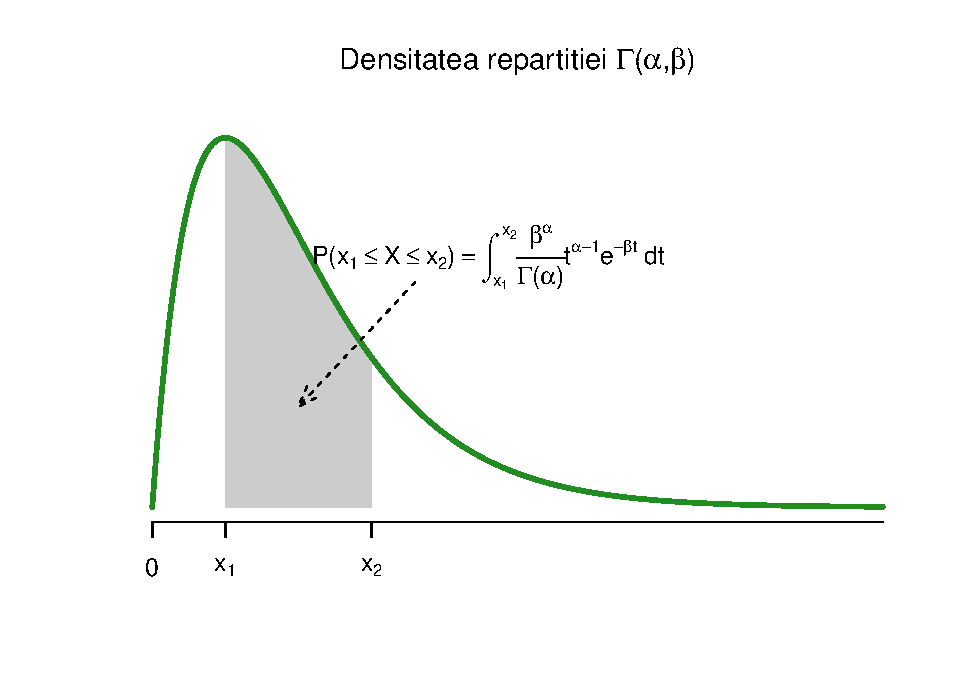
\includegraphics[width=0.7\linewidth]{Lab_1_files/figure-latex/unnamed-chunk-177-1} \end{center}

\begin{rmdexercise}
Arătați că funcția \(\Gamma(\alpha)\) verifică\footnote{Pentru mai multe
  proprietăți puteți consulta lucrarea lui E. Artin
  \href{http://plouffe.fr/simon/math/Artin\%20E.\%20The\%20Gamma\%20Function\%20(1931)(23s).pdf}{The
  Gamma Function}}:

\begin{enumerate}
\def\labelenumi{\arabic{enumi})}
\tightlist
\item
  \(\Gamma(1)=1\)
\item
  \(\Gamma(\alpha+1) = \alpha\Gamma(\alpha), \quad \forall \alpha>0\)
\item
  \(\Gamma(\alpha) = \beta^{\alpha}\int_{0}^{\infty}x^{\alpha-1} e^{- \beta x}\,dx,\quad \forall \alpha, \beta>0\)
\item
  \(\Gamma(n) = (n-1)!,\quad n = 1,2,\cdots\)
\item
  \(\Gamma(1/2) = \sqrt{\pi}\)
\end{enumerate}
\end{rmdexercise}

Pentru mai multe proprietăți ale funcției \(\Gamma(\alpha)\) puteți
consulta lucrarea (Artin 1964).

Funcția de repartiție a unei variabile aleatoare
\(X\sim \Gamma(\alpha, \beta)\) este dată de

\[
  F_{X}(x) = \int_{-\infty}^{x}f_X(t)\,dt = \frac{\beta^{\alpha}}{\Gamma(\alpha)}\int_{-\infty}^{x} t^{\alpha-1} e^{-\beta t}\,dt
\]

și nu are o formulă explicită de calcul.

\begin{center}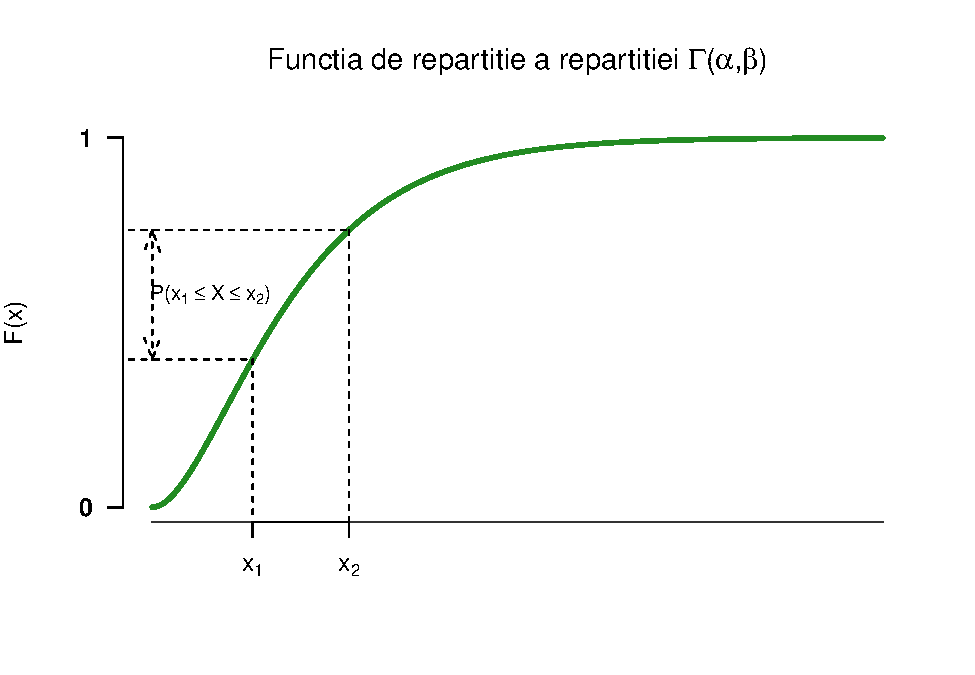
\includegraphics[width=0.7\linewidth]{Lab_1_files/figure-latex/unnamed-chunk-179-1} \end{center}

Observăm că repartiția \(\Gamma(1, \lambda)\) coincide cu repartiția
\(\mathcal{E}(\lambda)\).

Media și varianța variabilei aleatoare \(X\) repartizate Gama de
parametrii \(\Gamma(\alpha, \beta)\) sunt egale cu

\[
  \mathbb{E}[X] = \frac{\alpha}{\beta},\quad Var(X) = \frac{\alpha}{\beta^2}.
\]

\begin{rmdexercise}
Arătați că media și varianța unei variabile aleatoare repartizate Gama
de parametrii \(\alpha\) și \(\beta\) sunt egale cu

\[
  \mathbb{E}[X] = \frac{\alpha}{\beta},\quad Var(X) = \frac{\alpha}{\beta^2}. 
\]
\end{rmdexercise}

În R putem să

\begin{itemize}
\tightlist
\item
  generăm observații independente din repartiția
  \(\Gamma(\alpha, \beta)\) (e.g. \(\alpha = 2\), \(\beta = 2\))
\end{itemize}

\begin{Shaded}
\begin{Highlighting}[]
\KeywordTok{rgamma}\NormalTok{(}\DecValTok{15}\NormalTok{, }\DataTypeTok{shape =} \DecValTok{2}\NormalTok{, }\DataTypeTok{rate =} \DecValTok{2}\NormalTok{)}
\NormalTok{ [}\DecValTok{1}\NormalTok{] }\FloatTok{0.2739606} \FloatTok{1.0172288} \FloatTok{1.6546379} \FloatTok{0.4210210} \FloatTok{0.8476985} \FloatTok{0.2928765} \FloatTok{0.6798413}
\NormalTok{ [}\DecValTok{8}\NormalTok{] }\FloatTok{1.1393160} \FloatTok{1.0763898} \FloatTok{1.4411221} \FloatTok{0.9500644} \FloatTok{0.7387296} \FloatTok{0.4159926} \FloatTok{0.8942659}
\NormalTok{[}\DecValTok{15}\NormalTok{] }\FloatTok{0.8366199}
\end{Highlighting}
\end{Shaded}

\begin{itemize}
\tightlist
\item
  calculăm densitatea unei variabile aleatoare repartizate
  \(\Gamma(\alpha, \beta)\) în diferite puncte
\end{itemize}

\begin{Shaded}
\begin{Highlighting}[]
\KeywordTok{dgamma}\NormalTok{(}\KeywordTok{seq}\NormalTok{(}\DecValTok{0}\NormalTok{, }\DecValTok{5}\NormalTok{, }\DataTypeTok{length.out =} \DecValTok{20}\NormalTok{), }\DataTypeTok{shape =} \DecValTok{1}\NormalTok{, }\DataTypeTok{rate =} \DecValTok{3}\NormalTok{)}
\NormalTok{ [}\DecValTok{1}\NormalTok{] }\FloatTok{3.000000e+00} \FloatTok{1.362251e+00} \FloatTok{6.185761e-01} \FloatTok{2.808853e-01} \FloatTok{1.275455e-01}
\NormalTok{ [}\DecValTok{6}\NormalTok{] }\FloatTok{5.791632e-02} \FloatTok{2.629886e-02} \FloatTok{1.194188e-02} \FloatTok{5.422615e-03} \FloatTok{2.462321e-03}
\NormalTok{[}\DecValTok{11}\NormalTok{] }\FloatTok{1.118100e-03} \FloatTok{5.077110e-04} \FloatTok{2.305433e-04} \FloatTok{1.046860e-04} \FloatTok{4.753619e-05}
\NormalTok{[}\DecValTok{16}\NormalTok{] }\FloatTok{2.158541e-05} \FloatTok{9.801583e-06} \FloatTok{4.450739e-06} \FloatTok{2.021008e-06} \FloatTok{9.177070e-07}
\end{Highlighting}
\end{Shaded}

\begin{itemize}
\tightlist
\item
  calculăm funcția de repartiție a unei variabile repartizate
  \(\Gamma(\alpha, \beta)\) pentru diferite valori
\end{itemize}

\begin{Shaded}
\begin{Highlighting}[]
\KeywordTok{pgamma}\NormalTok{(}\KeywordTok{seq}\NormalTok{(}\DecValTok{0}\NormalTok{, }\DecValTok{5}\NormalTok{, }\DataTypeTok{length.out =} \DecValTok{15}\NormalTok{), }\DataTypeTok{shape =} \DecValTok{1}\NormalTok{, }\DataTypeTok{rate =} \DecValTok{3}\NormalTok{)}
\NormalTok{ [}\DecValTok{1}\NormalTok{] }\FloatTok{0.0000000} \FloatTok{0.6574811} \FloatTok{0.8826808} \FloatTok{0.9598160} \FloatTok{0.9862362} \FloatTok{0.9952856} \FloatTok{0.9983852}
\NormalTok{ [}\DecValTok{8}\NormalTok{] }\FloatTok{0.9994469} \FloatTok{0.9998106} \FloatTok{0.9999351} \FloatTok{0.9999778} \FloatTok{0.9999924} \FloatTok{0.9999974} \FloatTok{0.9999991}
\NormalTok{[}\DecValTok{15}\NormalTok{] }\FloatTok{0.9999997}
\end{Highlighting}
\end{Shaded}

\begin{itemize}
\tightlist
\item
  calculăm cuantilele de ordin \(p\in(0,1)\)
\end{itemize}

\begin{Shaded}
\begin{Highlighting}[]
\KeywordTok{qgamma}\NormalTok{(}\KeywordTok{c}\NormalTok{(}\FloatTok{0.01}\NormalTok{, }\FloatTok{0.025}\NormalTok{, }\FloatTok{0.05}\NormalTok{, }\FloatTok{0.25}\NormalTok{, }\FloatTok{0.5}\NormalTok{, }\FloatTok{0.75}\NormalTok{, }\FloatTok{0.95}\NormalTok{, }\FloatTok{0.975}\NormalTok{, }\FloatTok{0.99}\NormalTok{), }\DataTypeTok{shape =} \DecValTok{1}\NormalTok{, }\DataTypeTok{rate =} \DecValTok{3}\NormalTok{)}
\NormalTok{[}\DecValTok{1}\NormalTok{] }\FloatTok{0.003350112} \FloatTok{0.008439269} \FloatTok{0.017097765} \FloatTok{0.095894024} \FloatTok{0.231049060} \FloatTok{0.462098120}
\NormalTok{[}\DecValTok{7}\NormalTok{] }\FloatTok{0.998577425} \FloatTok{1.229626485} \FloatTok{1.535056729}
\end{Highlighting}
\end{Shaded}

\begin{rmdexercise}
Fie \(X\) o variabilă aleatoare repartizată \(\Gamma(\alpha, \beta)\).
Pentru fiecare pereche de parametrii \((\alpha, \beta)\) din mulțimea
\(\{(1,0.5), (2, 0.5), (3, 0.5), (5, 1), (9, 0.5), (7.5, 1), (0.5, 1) \}\)
trasați pe același grafic densitățile repartițiilor Gama cu parametrii
\((\alpha, \beta)\). Adăugați legendele corespunzătoare. Aceeași cerință
pentru funcțiile de repartiție.
\end{rmdexercise}

\begin{center}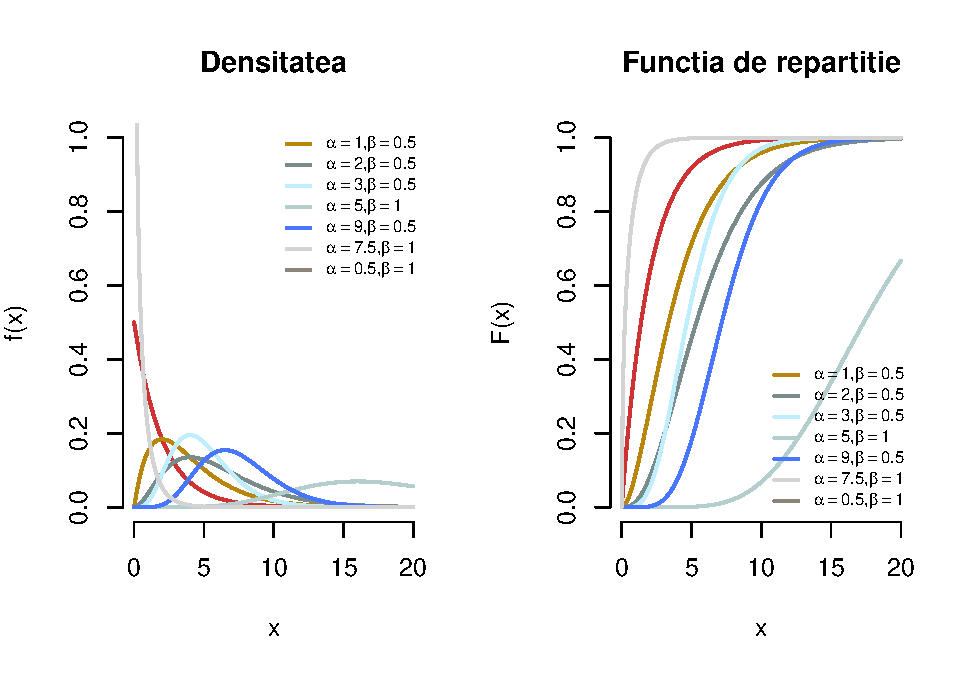
\includegraphics[width=0.7\linewidth]{Lab_1_files/figure-latex/unnamed-chunk-186-1} \end{center}

\begin{rmdexercise}
Generați \(250\) de observații din repartiția \(\Gamma(9,2)\), trasați
histograma acestora și suprapuneți densitatea repartiției date (vezi
figura de mai jos).
\end{rmdexercise}

\begin{center}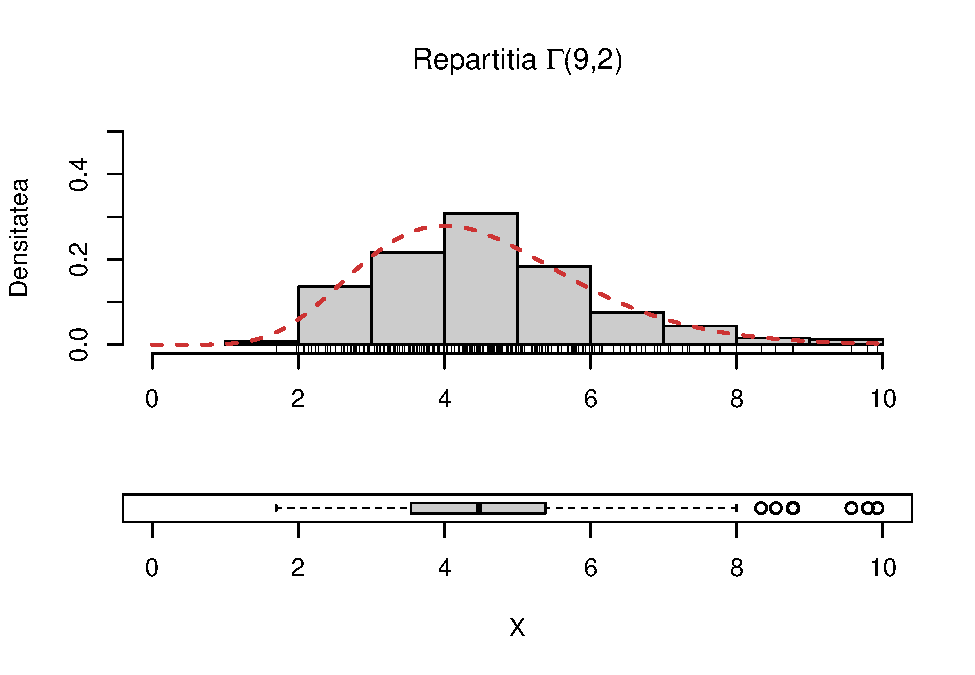
\includegraphics[width=0.7\linewidth]{Lab_1_files/figure-latex/unnamed-chunk-188-1} \end{center}

\subsection{Repartiția Beta}\label{repartitia-beta}

Spunem că o variabilă aleatoare \(X\) este repartizată \emph{Beta} de
parametrii \((\alpha, \beta)\), cu \(\alpha, \beta > 0\), și se notează
cu \(X\sim B(\alpha,\beta)\), dacă densitatea ei are forma

\[
  f_X(x) = \frac{1}{B(\alpha, \beta)} x^{\alpha-1} (1-x)^{\beta-1},\quad 0\leq x\leq 1.
\] unde \(B(\alpha, \beta)\) este funcția (Beta, numită și integrală
Euler de primul tip) definită prin

\[
  B(\alpha, \beta) = \int_{0}^{\infty}x^{\alpha-1} (1-x)^{\beta-1}\,dx,\quad \forall \alpha, \beta >0.
\]

\begin{center}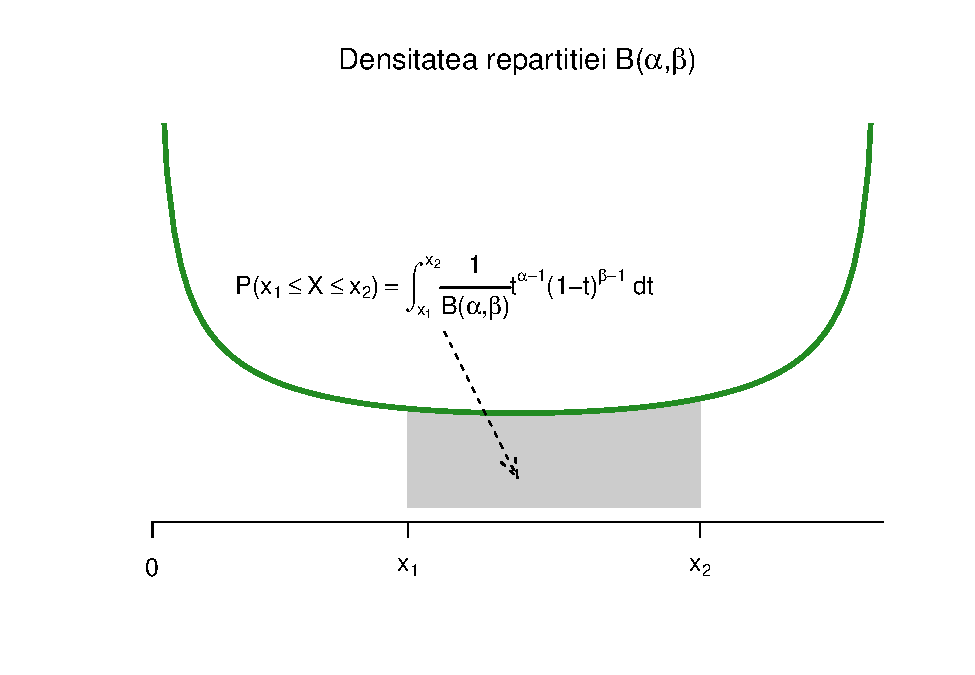
\includegraphics[width=0.7\linewidth]{Lab_1_files/figure-latex/unnamed-chunk-189-1} \end{center}

\begin{rmdexercise}
Arătați că funcția Beta \(B(\alpha, \beta)\) verifică următoarele
proprietăți:

\begin{enumerate}
\def\labelenumi{\arabic{enumi})}
\tightlist
\item
  \(B(\alpha, \beta) = \frac{\Gamma(\alpha)\Gamma(\beta)}{\Gamma(\alpha+\beta)}\)
\item
  \(B(\alpha, \beta) = B(\beta, \alpha)\)
\item
  \(B(\alpha, \beta) = B(\alpha, \beta+1) + B(\alpha+1, \beta)\)
\item
  \(B(\alpha + 1, \beta) = B(\alpha, \beta) \frac{\alpha}{\alpha+\beta}\)
  și
  \(B(\alpha, \beta + 1) = B(\alpha, \beta) \frac{\beta}{\alpha+\beta}\).
\end{enumerate}
\end{rmdexercise}

Funcția de repartiție a unei variabile aleatoare
\(X\sim B(\alpha, \beta)\) este dată de

\[
  F_{X}(x) = \int_{-\infty}^{x}f_X(t)\,dt = \frac{1}{B(\alpha, \beta)} \int_{-\infty}^{x} t^{\alpha-1} (1-t)^{\beta-1}\,dt
\]

și nu are o formulă explicită de calcul.

\begin{center}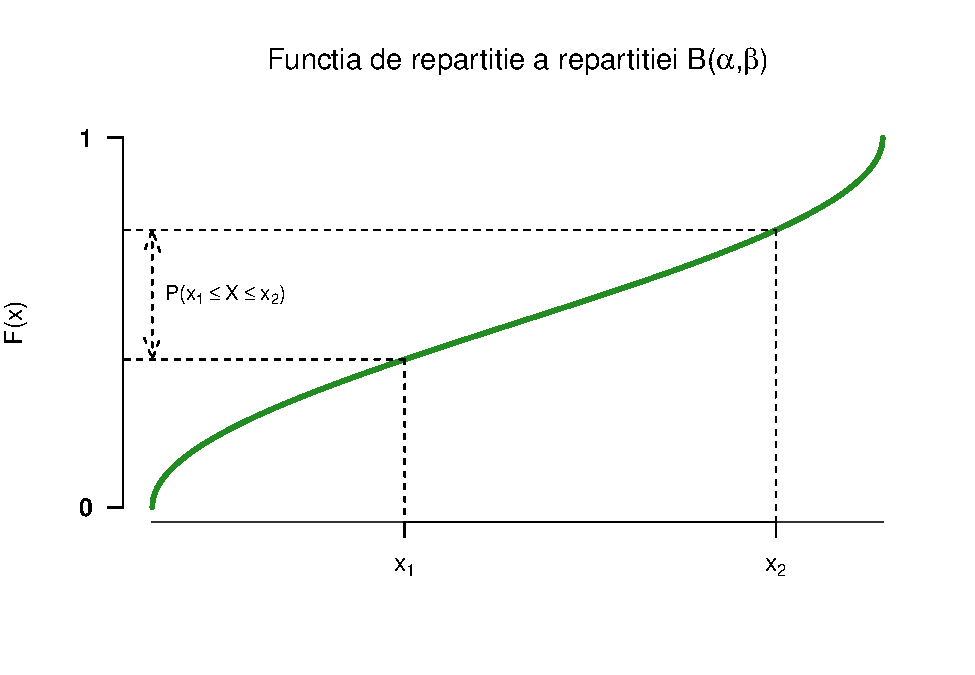
\includegraphics[width=0.7\linewidth]{Lab_1_files/figure-latex/unnamed-chunk-191-1} \end{center}

Observăm că repartiția \(B(1, 1)\) coincide cu repartiția
\(\mathcal{U}([0,1])\).

Media și varianța variabilei aleatoare \(X\) repartizate Gamma de
parametrii \(B(\alpha, \beta)\) sunt egale cu

\[
  \mathbb{E}[X] = \frac{\alpha}{\alpha+\beta},\quad Var(X) = \frac{\alpha\beta}{(\alpha+\beta)^2(\alpha+\beta+1)}.
\]

Observăm că \(Var(X)\leq\mathbb{E}[X](1-\mathbb{E}[X])\).

\begin{rmdexercise}
Arătați că media și varianța unei variabile aleatoare repartizate Beta
de parametrii \(\alpha\) și \(\beta\) sunt egale cu

\[
  \mathbb{E}[X] = \frac{\alpha}{\alpha+\beta},\quad Var(X) = \frac{\alpha\beta}{(\alpha+\beta)^2(\alpha+\beta+1)}. 
\]
\end{rmdexercise}

În R putem să

\begin{itemize}
\tightlist
\item
  generăm observații independente din repartiția \(B(\alpha, \beta)\)
  (e.g. \(\alpha = 2.5\), \(\beta = 1\))
\end{itemize}

\begin{Shaded}
\begin{Highlighting}[]
\KeywordTok{rbeta}\NormalTok{(}\DecValTok{15}\NormalTok{, }\DataTypeTok{shape1 =} \FloatTok{2.5}\NormalTok{, }\DataTypeTok{shape2 =} \DecValTok{1}\NormalTok{)}
\NormalTok{ [}\DecValTok{1}\NormalTok{] }\FloatTok{0.7945436} \FloatTok{0.7609136} \FloatTok{0.9265073} \FloatTok{0.9309420} \FloatTok{0.5621874} \FloatTok{0.3664261} \FloatTok{0.9694945}
\NormalTok{ [}\DecValTok{8}\NormalTok{] }\FloatTok{0.5804873} \FloatTok{0.9504669} \FloatTok{0.9115169} \FloatTok{0.8457509} \FloatTok{0.6717780} \FloatTok{0.7213322} \FloatTok{0.9738473}
\NormalTok{[}\DecValTok{15}\NormalTok{] }\FloatTok{0.9791769}
\end{Highlighting}
\end{Shaded}

\begin{itemize}
\tightlist
\item
  calculăm densitatea unei variabile aleatoare repartizate
  \(B(\alpha, \beta)\) în diferite puncte
\end{itemize}

\begin{Shaded}
\begin{Highlighting}[]
\KeywordTok{dbeta}\NormalTok{(}\KeywordTok{seq}\NormalTok{(}\DecValTok{0}\NormalTok{, }\DecValTok{1}\NormalTok{, }\DataTypeTok{length.out =} \DecValTok{20}\NormalTok{), }\DataTypeTok{shape1 =} \DecValTok{1}\NormalTok{, }\DataTypeTok{shape2 =} \DecValTok{3}\NormalTok{)}
\NormalTok{ [}\DecValTok{1}\NormalTok{] }\FloatTok{3.000000000} \FloatTok{2.692520776} \FloatTok{2.401662050} \FloatTok{2.127423823} \FloatTok{1.869806094}
\NormalTok{ [}\DecValTok{6}\NormalTok{] }\FloatTok{1.628808864} \FloatTok{1.404432133} \FloatTok{1.196675900} \FloatTok{1.005540166} \FloatTok{0.831024931}
\NormalTok{[}\DecValTok{11}\NormalTok{] }\FloatTok{0.673130194} \FloatTok{0.531855956} \FloatTok{0.407202216} \FloatTok{0.299168975} \FloatTok{0.207756233}
\NormalTok{[}\DecValTok{16}\NormalTok{] }\FloatTok{0.132963989} \FloatTok{0.074792244} \FloatTok{0.033240997} \FloatTok{0.008310249} \FloatTok{0.000000000}
\end{Highlighting}
\end{Shaded}

\begin{itemize}
\tightlist
\item
  calculăm funcția de repartiție a unei variabile repartizate
  \(B(\alpha, \beta)\) pentru diferite valori
\end{itemize}

\begin{Shaded}
\begin{Highlighting}[]
\KeywordTok{pbeta}\NormalTok{(}\KeywordTok{seq}\NormalTok{(}\DecValTok{0}\NormalTok{, }\DecValTok{1}\NormalTok{, }\DataTypeTok{length.out =} \DecValTok{15}\NormalTok{), }\DataTypeTok{shape1 =} \DecValTok{1}\NormalTok{, }\DataTypeTok{shape2 =} \DecValTok{3}\NormalTok{)}
\NormalTok{ [}\DecValTok{1}\NormalTok{] }\FloatTok{0.0000000} \FloatTok{0.1993440} \FloatTok{0.3702624} \FloatTok{0.5149417} \FloatTok{0.6355685} \FloatTok{0.7343294} \FloatTok{0.8134111}
\NormalTok{ [}\DecValTok{8}\NormalTok{] }\FloatTok{0.8750000} \FloatTok{0.9212828} \FloatTok{0.9544461} \FloatTok{0.9766764} \FloatTok{0.9901603} \FloatTok{0.9970845} \FloatTok{0.9996356}
\NormalTok{[}\DecValTok{15}\NormalTok{] }\FloatTok{1.0000000}
\end{Highlighting}
\end{Shaded}

\begin{itemize}
\tightlist
\item
  calculăm cuantilele de ordin \(p\in(0,1)\)
\end{itemize}

\begin{Shaded}
\begin{Highlighting}[]
\KeywordTok{qbeta}\NormalTok{(}\KeywordTok{c}\NormalTok{(}\FloatTok{0.01}\NormalTok{, }\FloatTok{0.025}\NormalTok{, }\FloatTok{0.05}\NormalTok{, }\FloatTok{0.25}\NormalTok{, }\FloatTok{0.5}\NormalTok{, }\FloatTok{0.75}\NormalTok{, }\FloatTok{0.95}\NormalTok{, }\FloatTok{0.975}\NormalTok{, }\FloatTok{0.99}\NormalTok{), }\DataTypeTok{shape1 =} \DecValTok{1}\NormalTok{, }\DataTypeTok{shape2 =} \DecValTok{3}\NormalTok{)}
\NormalTok{[}\DecValTok{1}\NormalTok{] }\FloatTok{0.003344507} \FloatTok{0.008403759} \FloatTok{0.016952428} \FloatTok{0.091439704} \FloatTok{0.206299474} \FloatTok{0.370039475}
\NormalTok{[}\DecValTok{7}\NormalTok{] }\FloatTok{0.631596850} \FloatTok{0.707598226} \FloatTok{0.784556531}
\end{Highlighting}
\end{Shaded}

\begin{rmdexercise}
Fie \(X\) o variabilă aleatoare repartizată \(B(\alpha, \beta)\). Pentru
fiecare pereche de parametrii \((\alpha, \beta)\) din mulțimea
\(\{(0.5,0.5), (1, 3), (5, 1), (2, 2), (2, 5)\}\) trasați pe același
grafic densitățile repartițiilor Beta cu parametrii \((\alpha, \beta)\).
Adăugați legendele corespunzătoare. Aceeași cerință pentru funcțiile de
repartiție.
\end{rmdexercise}

\begin{center}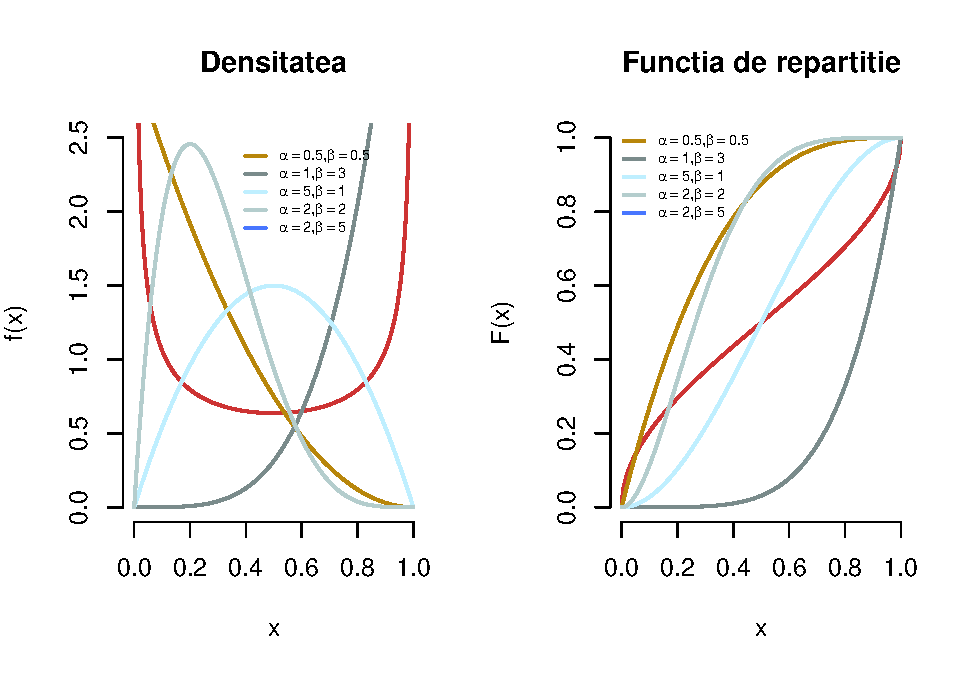
\includegraphics[width=0.7\linewidth]{Lab_1_files/figure-latex/unnamed-chunk-198-1} \end{center}

\begin{rmdexercise}
Generați \(250\) de observații din repartiția \(B(3,3)\), trasați
histograma acestora și suprapuneți densitatea repartiției date (vezi
figura de mai jos).
\end{rmdexercise}

\begin{center}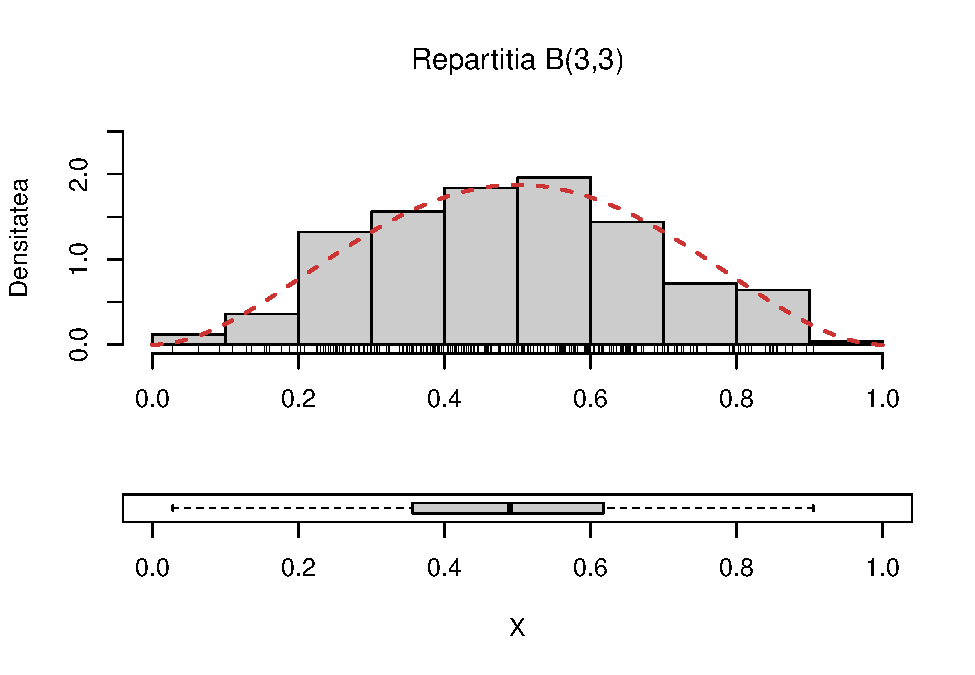
\includegraphics[width=0.7\linewidth]{Lab_1_files/figure-latex/unnamed-chunk-200-1} \end{center}

\section*{Referințe}\label{referinte}
\addcontentsline{toc}{section}{Referințe}

\hypertarget{refs}{}
\hypertarget{ref-Artin1964}{}
Artin, Emil. 1964. ``The Gamma Function.'' Athena Series - Selected
topics in mathematics.
\url{http://plouffe.fr/simon/math/Artin\%20E.\%20The\%20Gamma\%20Function\%20(1931)(23s).pdf}.

\hypertarget{ref-Johnson1994}{}
Johnson, N., S. Kotz, and N. Balakrishnan. 1994. \emph{Continuous
Univariate Distributions}. 2nd ed. Vol. 1. John Wiley \& Sons, New York.

\hypertarget{ref-LinBai2010}{}
Lin, Z., and Z. Bai. 2010. \emph{Probability Inequalities}. Springer.


\end{document}
